%*************************************************************************************************************
% PREAMBLE STUFF
%*************************************************************************************************************
% Instead of inserting my \usepackage and defined commands here, I keep them in a separate file
% Queen's Thesis Format
% (Borrowed from Dean Jin's BigDis.tex file, then heavily modified :)

% Michelle L. Crane, Queen's University, 2003

%*************************************************************************************************************
% DOCUMENT STYLE
%*************************************************************************************************************
\documentclass[12pt]{report}
%-------------------------------------------------------------------------------------------------------------
\usepackage{quthesis}        % the Queen's University dissertation style file
                             % Note:  In my thesis, I had many Listings, so I
                             % tweaked the old quthesis sty file to create a
                             % List of Listings in the table of contents.
                             % However, this version of quthesis does *not*
                             % include these modifications.
%\usepackage[sectionbib]{natbib}
%\usepackage{chapterbib}  
\usepackage{chapterbib}

\usepackage{listings}
\usepackage{color}
\usepackage{longtable}


%I don't even use the fancyheadings - it looks nice enough without it
%\usepackage{fancyheadings}  % doesn't seem to change the headings at all!
%*************************************************************************************************************

\usepackage{hyperref}

%*************************************************************************************************************
% SPACING
%*************************************************************************************************************
\usepackage{setspace}        % for use of \singlespacing and \doublespacing
%*************************************************************************************************************


%*************************************************************************************************************
% HEADINGS
%*************************************************************************************************************

% This changes the headings go that they are prettier, this can be commented out for traditional headings.
%\usepackage{sectsty}
%\allsectionsfont{\bfseries}% set all the section font to bfseries
%\chapterfont{\centering\Large} % set the sizes of chapters, sections ...
%\sectionfont{\normalsize}
%\subsectionfont{\normalsize}

% for formatting Table of Contents entry, example: Chapter 1 Introduction
\usepackage[subfigure]{tocloft}
\usepackage{tocloft}
\renewcommand{\cftchappresnum}{Chapter }
\renewcommand{\cftchapaftersnum}{:}
\renewcommand{\cftchapnumwidth}{7em}

% for formatting Table of Contents entry for Appendix, example: Appendix 1: Stuff
\newcommand*\updatechaptername{%
   \addtocontents{toc}{\protect\renewcommand*\protect\cftchappresnum{Appendix }}
}

%*************************************************************************************************************
% FOOTNOTES
%*************************************************************************************************************

\interfootnotelinepenalty=10000 % This line stops footnotes from splitting onto two pages.

%*************************************************************************************************************
% VERBATIM
%*************************************************************************************************************
\usepackage{moreverb}        % Using this package to get better control of the
                             % verbatim environment, mostly for the use of the
                             % listing environment which puts line number
                             % beside each line.  Note that there has to be a number
                             % in each set of brackets, i.e., \begin{listing}[1]{1}.
                             % PDF info file is "The moreverb package" by
                             % Robin Fairbairns (rf@cl.cam.ac.uk) after
                             % Angus Duggan, Rainer Schopf and Victor Eijkhout, 2000/06/29.
%-------------------------------------------------------------------------------------------------------------
%\usepackage{verbatim}        % allows the use of \begin{comment} and \end{comment}
                             % as well as \verbatiminput{file}
                             % Note:  when using verbatim to input from a text file,
                             % such as a specification or code, use \begin{singlespacing}
                             % and \end{singlespacing}.  Also, tabs are not read
                             % properly, so the input file must only use spaces.

%                             \begin{comment}
%                             Can also use the verbatim package for
%                             comments like this...
%                             \end{comment}
%*************************************************************************************************************


%*************************************************************************************************************
% GLOSSARY
% Using a glossary is more than beginners need to know; leaving the packages, etc. here for now.
%*************************************************************************************************************
%\usepackage[nonumberlist]{glossaries} % use glossaries since glossary package is out dated
%\makeglossaries  % tell latex to make the glossary
%\glossarystyle{list}

%*************************************************************************************************************


%*************************************************************************************************************
% INDEX
% Also possible to make an index; didn't use for my thesis.
%*************************************************************************************************************
%\usepackage{makeidx}         % to make the index
%-------------------------------------------------------------------------------------------------------------
% Tell Latex to make an index
%\makeindex
%*************************************************************************************************************


%*************************************************************************************************************
% MATH STUFF
%*************************************************************************************************************
\usepackage{amsmath}         % to make nice equations
\usepackage{amssymb} 

%-------------------------------------------------------------------------------------------------------------
\usepackage{amsthm}          % to make nice theorem, i.e., definition

% Using the amsthm package, define a new theorem environment for my
% definition.  * means don't number it.
\newtheorem*{definition}{Definition}
%-------------------------------------------------------------------------------------------------------------
\usepackage{cases}           % to make numbered cases (equations)
%-------------------------------------------------------------------------------------------------------------
\usepackage{calc}            % Used with the Ventry environment defined below.
%*************************************************************************************************************


%*************************************************************************************************************
% FLOATS AND FIGURES
%*************************************************************************************************************
\usepackage{graphicx}        % for graphic images (use \includegraphics[...]{file.eps})
%-------------------------------------------------------------------------------------------------------------
%\usepackage{subfigure}       % for subfigures (figures within figures)
\usepackage{subfig}
%-------------------------------------------------------------------------------------------------------------
\usepackage{boxedminipage}   % to make boxed minipages, i.e., boxes around figures
%-------------------------------------------------------------------------------------------------------------
\usepackage{rotate}          % for use of \begin{sideways} and \end{sideways}
%-------------------------------------------------------------------------------------------------------------
\usepackage{float}           % Using this package to get better control of my floats
                             % including the ability to define new float types for
                             % my specification and code listings.
                             % DVI info file is "An Improved Environment for Floats"
                             % by Anselm Lingnau, lingnau@tm.informatik.uni=frankfurt.de
                             % 1995/03/29.

% Define new float styles here
% Ruled style for examples
%\floatstyle{ruled}
%\newfloat{Example}{h}{lop}[chapter]

% Style of float used for code listings
\floatstyle{ruled}
\newfloat{Listing}{H}{lis}[chapter]

                             % Note:  The listings don't have space between the chapters, unlike
                             % the standard list of tables etc.  At the end, copy the spacing
                             % commands from the .toc file and insert into the .lis file.  Then,
                             % DO NOT LATEX it again, simply go to the DVI viewer!
%*************************************************************************************************************
% TABLES
%*************************************************************************************************************
\usepackage{tabularx}        % Package used to make variable width-columns, i.e.,
                             % column widths are changed to fit the maximum width
                             % and text is wrapped nicely.

\usepackage{threeparttable}
\usepackage{rotating}

%*************************************************************************************************************
% CAPTIONS
%*************************************************************************************************************
%\usepackage[hang]{caption}   % Package used to make my captions 'hang', i.e., wrap
                             % around, but not under the name of the caption.
%-------------------------------------------------------------------------------------------------------------
% Find that the captions are too far from my verbatim figures, but if
% I change it to 0, then the captions are too close for my other types
% of figures.  Maybe set each one separately?
%\setlength{\abovecaptionskip}{1ex}

%\setlength{\textfloatsep}{1ex plus1pt minus1pt}

%\setlength{\intextsep}{1ex plus1pt minus1pt}

%\setlength{\floatsep}{1ex plus1pt minus1pt}
%*************************************************************************************************************


%*************************************************************************************************************
% MISCELLANEOUS
%*************************************************************************************************************
\usepackage{layout}          % useful for determining the margins of a document
                             % use with \layout command
%-------------------------------------------------------------------------------------------------------------
\usepackage{changebar}       % Way of indicating modifications by putting bars in the
                             % margin.  Read about it in "The Latex Companion".
%*************************************************************************************************************


%*************************************************************************************************************
% REFERENCES ETC.
%*************************************************************************************************************
\usepackage{varioref}        % Better page references, e.g., "on preceding page", etc.
                             % \vref{key} Create an enhanced reference.
                             % \vpageref[text]{key} Create an enhanced page reference.
                             % \vrefrange{key}{key} Create an enhanced range of references.
                             % \vpagerefrange[text]{key}{key} Create an enhanced range of page references.
                             % Note: doesn't really work for consecutive pages.

% Renewing the text for before and after, because I don't like the default flip-flopping one.
% And 'on the page before' sounds dumb!

\renewcommand{\reftextafter}{on the next page}
\renewcommand{\reftextbefore}{on the previous page}
%-------------------------------------------------------------------------------------------------------------
\usepackage{url}             % for use of \url - pretty web addresses
%*************************************************************************************************************
% HYPERLINKS (must be last)
%*************************************************************************************************************
%\usepackage[]{hyperref}
%\usepackage[dvips,bookmarks]{hyperref}
                             % Neat package to turn href, ref, cite, gloss entries
                             % into hyperlinks in the dvi file.
                             % Make sure this is the last package loaded.
                             % Use with dvips option to get hyperlinks to work in ps and pdf
                             % files.  Unfortunately, then they don't work in the dvi file!
                             % Use without the dvips option to get the links to work in the dvi file.
                             % Note:  \floatstyle{ruled} don't work properly; so change to plain.
                             % Not as pretty, but functional...
                             % The bookmarks option sets up proper bookmarks in the pdf file :)

% Need this command to allow hyperref to play nicely with gloss; otherwise
% almost every \gloss will cause an error...
%\renewcommand{\glosslinkborder}{0 0 0}
%*************************************************************************************************************


%*************************************************************************************************************
% MISCELLANEOUS COMMANDS AND ENVIRONMENTS
%*************************************************************************************************************
% Use this command to show more table of contents - used when playing
% with the draft outline
% I think it should be about 2???
\setcounter{tocdepth}{2}
%*************************************************************************************************************
% Environment definition I found in the "The Latex Companion".  Used to
% create a list environment where the indenting is the same for all of the
% entries, regardless of their length.  Note:  must \usepackage{calc}.
\newenvironment{Ventry}[1]%
    {\begin{list}{}{\renewcommand{\makelabel}[1]{\textbf{##1}\hfil}%
        \settowidth{\labelwidth}{\textbf{#1:}}%
        \setlength{\leftmargin}{\labelwidth+\labelsep}}}%
    {\end{list}}
%*************************************************************************************************************

%*************************************************************************************************************
% MY DEFINED COMMANDS
%*************************************************************************************************************
% Command that I can use to create notes in the margins;
% adapted from Juergen's META tag
%\newcommand{\meta}[1]{\begin{singlespacing}
%{\marginpar{\emph{\footnotesize Note: #1}}}\end{singlespacing}}
%*************************************************************************************************************
% Command that I can use to create lined headings
%\newcommand{\heading}[1]{\bigskip \hrule \smallskip \noindent \texttt{#1} \smallskip \hrule}
%*************************************************************************************************************
% Command that I can use for reading in a file, verbatim, with line
% numbers printed along the left side.  The parameter is the file name.
%\newcommand{\fileinnum}[1]{
%    \begin{singlespacing} {\footnotesize
%    \begin{listinginput}[1]{1}{#1}\end{listinginput}
%    }\end{singlespacing}
%}
%*************************************************************************************************************
% Command that I can use for reading in a file, verbatim, with NO line
% numbers, but in a smaller font.  The parameter is the file name.
\newcommand{\filein}[1]{
   \begin{singlespacing}{\footnotesize
    \begin{verbatiminput}{#1}\end{verbatiminput}
    }\end{singlespacing}
}
%*************************************************************************************************************
% Command that I can use for reading in a file, verbatim, with NO line
% numbers, but in a smaller font.  The parameter is the file name.
\newcommand{\fileinsmall}[1]{
    \begin{singlespacing}{\scriptsize
    \begin{verbatiminput}{#1}\end{verbatiminput}
    }\end{singlespacing}
}
%*************************************************************************************************************
% Dean't 'notesbox' command.  Needs setspace package.
%   Usage: \notesbox{This is a note.}
%%
\newcommand{\notesbox}[1]{
     \ \\
      \singlespacing
      \noindent\begin{boxedminipage}[h]{\textwidth}{\sf{#1}}\end{boxedminipage}
      \doublespacing
}


% Standard journal abbreviations
% Mostly as used by ADS, with a few additions for journals where MNRAS does not
% follow normal IAU style.

\newcommand\aap{A\&A}                % Astronomy and Astrophysics
\let\astap=\aap                          % alternative shortcut
\newcommand\aapr{A\&ARv}             % Astronomy and Astrophysics Review (the)
\newcommand\aaps{A\&AS}              % Astronomy and Astrophysics Supplement Series
\newcommand\actaa{Acta Astron.}      % Acta Astronomica
\newcommand\afz{Afz}                 % Astrofizika
\newcommand\aj{AJ}                   % Astronomical Journal (the)
\newcommand\ao{Appl. Opt.}           % Applied Optics
\let\applopt=\ao                         % alternative shortcut
\newcommand\aplett{Astrophys.~Lett.} % Astrophysics Letters
\newcommand\apj{ApJ}                 % Astrophysical Journal
\newcommand\apjl{ApJ}                % Astrophysical Journal, Letters
\let\apjlett=\apjl                       % alternative shortcut
\newcommand\apjs{ApJS}               % Astrophysical Journal, Supplement
\let\apjsupp=\apjs                       % alternative shortcut
% The following journal does not appear to exist! Disabled.
%\newcommand\apspr{Astrophys.~Space~Phys.~Res.} % Astrophysics Space Physics Research
\newcommand\apss{Ap\&SS}             % Astrophysics and Space Science
\newcommand\araa{ARA\&A}             % Annual Review of Astronomy and Astrophysics
\newcommand\arep{Astron. Rep.}       % Astronomy Reports
\newcommand\aspc{ASP Conf. Ser.}     % ASP Conference Series
\newcommand\azh{Azh}                 % Astronomicheskii Zhurnal
\newcommand\baas{BAAS}               % Bulletin of the American Astronomical Society
\newcommand\bac{Bull. Astron. Inst. Czechoslovakia} % Bulletin of the Astronomical Institutes of Czechoslovakia 
\newcommand\bain{Bull. Astron. Inst. Netherlands} % Bulletin Astronomical Institute of the Netherlands
\newcommand\caa{Chinese Astron. Astrophys.} % Chinese Astronomy and Astrophysics
\newcommand\cjaa{Chinese J.~Astron. Astrophys.} % Chinese Journal of Astronomy and Astrophysics
\newcommand\fcp{Fundamentals Cosmic Phys.}  % Fundamentals of Cosmic Physics
\newcommand\gca{Geochimica Cosmochimica Acta}   % Geochimica Cosmochimica Acta
\newcommand\grl{Geophys. Res. Lett.} % Geophysics Research Letters
\newcommand\iaucirc{IAU~Circ.}       % IAU Cirulars
\newcommand\icarus{Icarus}           % Icarus
\newcommand\japa{J.~Astrophys. Astron.} % Journal of Astrophysics and Astronomy
\newcommand\jcap{J.~Cosmology Astropart. Phys.} % Journal of Cosmology and Astroparticle Physics
\newcommand\jcp{J.~Chem.~Phys.}      % Journal of Chemical Physics
\newcommand\jgr{J.~Geophys.~Res.}    % Journal of Geophysics Research
\newcommand\jqsrt{J.~Quant. Spectrosc. Radiative Transfer} % Journal of Quantitiative Spectroscopy and Radiative Transfer
\newcommand\jrasc{J.~R.~Astron. Soc. Canada} % Journal of the RAS of Canada
\newcommand\memras{Mem.~RAS}         % Memoirs of the RAS
\newcommand\memsai{Mem. Soc. Astron. Italiana} % Memoire della Societa Astronomica Italiana
\newcommand\mnassa{MNASSA}           % Monthly Notes of the Astronomical Society of Southern Africa
\newcommand\mnras{MNRAS}             % Monthly Notices of the Royal Astronomical Society
\newcommand\na{New~Astron.}          % New Astronomy
\newcommand\nar{New~Astron.~Rev.}    % New Astronomy Review
\newcommand\nat{Nature}              % Nature
\newcommand\nphysa{Nuclear Phys.~A}  % Nuclear Physics A
\newcommand\pra{Phys. Rev.~A}        % Physical Review A: General Physics
\newcommand\prb{Phys. Rev.~B}        % Physical Review B: Solid State
\newcommand\prc{Phys. Rev.~C}        % Physical Review C
\newcommand\prd{Phys. Rev.~D}        % Physical Review D
\newcommand\pre{Phys. Rev.~E}        % Physical Review E
\newcommand\prl{Phys. Rev.~Lett.}    % Physical Review Letters
\newcommand\pasa{Publ. Astron. Soc. Australia}  % Publications of the Astronomical Society of Australia
\newcommand\pasp{PASP}               % Publications of the Astronomical Society of the Pacific
\newcommand\pasj{PASJ}               % Publications of the Astronomical Society of Japan
\newcommand\physrep{Phys.~Rep.}      % Physics Reports
\newcommand\physscr{Phys.~Scr.}      % Physica Scripta
\newcommand\planss{Planet. Space~Sci.} % Planetary Space Science
\newcommand\procspie{Proc.~SPIE}     % Proceedings of the Society of Photo-Optical Instrumentation Engineers
\newcommand\rmxaa{Rev. Mex. Astron. Astrofis.} % Revista Mexicana de Astronomia y Astrofisica
\newcommand\qjras{QJRAS}             % Quarterly Journal of the RAS
\newcommand\sci{Science}             % Science
\newcommand\skytel{Sky \& Telesc.}   % Sky and Telescope
\newcommand\solphys{Sol.~Phys.}      % Solar Physics
\newcommand\sovast{Soviet~Ast.}      % Soviet Astronomy (aka Astronomy Reports)
\newcommand\ssr{Space Sci. Rev.}     % Space Science Reviews
\newcommand\zap{Z.~Astrophys.}       % Zeitschrift fuer Astrophysik



% Extra includes 

\usepackage{natbib}
\usepackage[outdir=./]{epstopdf}

%*************************************************************************************************************
% INCLUDE ONLY
%*************************************************************************************************************
% Use if you want to include only certain parts of the document, example \includeonly{introduction}
% in order to speed up compile time when you're focussing on some particular part.
%\includeonly{}


%*************************************************************************************************************
% DOCUMENT
%*************************************************************************************************************
\newcommand{\zrms}{z_{\rm rms}}
\newcommand{\zeff}{z_{\rm rms,eff}}
\renewcommand{\thepage}{}
%\newcommand{\last_page_of_biblio}{\def \last_page_number \numpages}
%\newcommand{\stitch_to_last_chapter}{\setcounter{page}{\last_page_number}}

\begin{document}

%*************************************************************************************************************
% TITLE
%*************************************************************************************************************

\title{Nature or Nurture? Collisionless Evolution of Galactic Disc-Halo Systems}

\author{J S Bauer}

\dept{Department of Physics}
\degree{Doctor of Philosophy}

% OPTIONAL HERE
% ~~~~~~~~~~~~~
% \submitdate{month year in which submitted to GPO}
%        - date LaTeX'd if omitted
% \copyrightyear{ear degree conferred}
%        - year LaTeX'd if omitted
% \figurespagetrue or \figurespagefalse
%        - produce or don't produce a List of Figures page (true by default)
% \tablespagetrue or \tablespagefalse
%        - produce or don't produce a List of Tables page (true by default)

\beforepreface

% Adding single spacing so abstract and table of contents is single spaced.

\begin{center}
\vspace*{\stretch{1}}
\noindent To Mom and Dad. Thank you for supporting me when I have been hard to support.

-- Your Loving Son
\vspace*{\stretch{1}}
\end{center}

\clearpage 

%{
%\noindent }%*************************************************************************************************************
% ABSTRACT
%*************************************************************************************************************

\prefacesection{Abstract}

In this thesis, we develop and apply a novel algorithm to understand 
the evolution of stellar discs in $\Lambda$CDM cosmological haloes.
Three main scientific areas are addressed: the effects of evolving stellar
discs on their host haloes, understanding bar formation in cosmological settings,
and the formation of vertical disc structure in response to the host halo.

First, we find that the presence of central concentrations of baryons in dark 
matter haloes enhances adiabatic contraction causes an overall modest 
reduction in substructure. Additionally, the detailed evolution of stellar discs 
is important for the inner halo density distribution. However,
properties of the halo such as the subhalo mass function are broadly unaffected
by the evolution of a realistic stellar disc.


Next, we find that stellar bars invariably form in Milky Way-like galaxies. The 
strength of these bars is less dependent on properties like the dynamical
temperature of the disc in a cosmological setting. Instead, the disc thickness
plays a leading role in determining the overall bar strength. Our discs
undergo notable buckling events, yielding present-day pseudobulge-disc-halo
systems. We show that these are qualitatively similar to the observed Milky Way.

Finally, we show that a wide variety of vertical structure forms when 
stellar discs are embedded in cosmological haloes. We further show that through
a variety of mechanisms, similar vertical structure is excited. By examining
twelve simulations of discs in cosmological haloes, we show that the Sgr dSph
need not be as massive as $10^{11}\,M_\odot$ to be consistent with observed
vertical structure in the Milky Way. In fact, the recent buckling of the Milky Way's
bar and its present interaction with the LMC are more likely culprits for some of
the observed structure in the Milky Way's thin disc.

%*************************************************************************************************************
% CO-AUTHORSHIP (if necessary)
%*************************************************************************************************************

%\prefacesection{Co-Authorship}



%*************************************************************************************************************
% STATEMENT OF ORIGINALITY (required CHEM, CISC, GEOL, MATH, PHYS (Ph.D. only))
%*************************************************************************************************************

\prefacesection{Statement of Originality}

The research presented in this thesis was completed under the supervision of Prof.
Lawrence M. Widrow at Queen’s University. All of the work presented here was done
by the author (Jacob S. Bauer) except where explicitly stated otherwise.

Chapter~\ref{ch:paper_i} contains a reproduction of a paper published in  Monthly Notices of the
Royal Astronomical Society as: Jacob S. Bauer, Lawrence M. Widrow, and Denis Erkal. Disc-halo interactions in $\Lambda$CDM. \textit{Monthly Notices of the Royal Astronomical Society}, 476:198-209,
2018. For this paper, I ran all of the simulations. The writing is mine with direct input from Lawrence M. Widrow and Denis Erkal. I performed all of the calculations. The analysis was handled primarily by me under the direction of Lawrence M. Widrow, with substantial input from Denis Erkal.

Chapter~\ref{ch:paper_ii} contains a reproduction of a paper published in  Monthly Notices of the
Royal Astronomical Society as: Jacob S. Bauer and Lawrence M. Widrow. Can stellar discs in a cosmological setting avoid forming strong bars?. \textit{Monthly Notices of the Royal Astronomical Society}, 476:523-537,
2019. For this paper, I ran all of the simulations. The writing is mine with direct input from Lawrence M. Widrow. I performed all of the calculations, except the one in \S2.3 which was performed by Lawrence M. Widrow. Figures 2-4 were also the work of Lawrence M. Widrow. The analysis was handled primarily by me under the direction of Lawrence M. Widrow.

Chapter~\ref{ch:paper_iii} contains a draft of a paper in preparation to be submitted to Monthly Notices of the Royal Astronomical Society. The working title for the paper is ``Vertical Structure and Kicked-Up Stars in $\Lambda$CDM Galaxies". For this work, I performed all of the simulations and writing. The analysis was handled primarily by me under the direction of Lawrence M. Widrow.

%*************************************************************************************************************
% ACKNOWLEDGEMENTS
%*************************************************************************************************************


\prefacesection{Acknowledgments}

As I reach the end of this chapter of my life, I know that I did not reach this milestone unassisted. Here, I recognize those who have helped me in this accomplishment.

I want to acknowledge, first and foremost, the amazing supervision I received from Larry Widrow. His careful, unyielding approach to scientific research has not only shown me how to be a better scientist, but a more conscientious communicator. I am immensely grateful for the opportunity to work with him, and for the years of guidance that will serve me well for the rest of my life.

In addition to Larry, I want to acknowledge my other mentors, Heidi Newberg and Denis Erkal. Through my work with each of them, I learned how to evaluate myself more honestly, both professionally and personally. I am grateful that through my work with my mentors, I learned to be simultaneously self-critical and able to forgive myself for mistakes. Without Heidi's and Denis' guidance, I would not have been able to finish this work.

To all of the other faculty members and Department staff, I am tremendously grateful for your contributions to me personally, and to the program as a whole. I am proud of my friends and colleagues at Queen's, and it is through your hard work that this positive academic environment exists. I wish you all the best.

I am grateful for the years of friendship with my fellow astronomy graduate students. In their own ways, they have all kept me mostly sane for 4 years. I would not have been able to persevere without their support. Although they did not succeed in turning me into a Canadian, they did manage to make me grow a beard. I look forward to many more years of friendship.

I want to acknowledge my wonderful family for their support. Mom and Dad have been my biggest supporters through the ups and downs, and this thesis is as much their accomplishment as it is mine. 

I am grateful to Rachel Peckman, Chris Weir, and Taylor Weir for our lasting friendships. In high school, Chris showed me that I was capable of pursuing science. Our adventures in Tech Club (RIP), our shenanigans at RPI (RIP), and subsequent friendship (not RIP) made me strive to be a better technologist and person.

Lastly, I want to acknowledge my partner, Alexis Hill. I can't wait to see what adventures life hold for us in Austin. I wouldn't want to be on this roller coaster called life with anyone else.



\singlespacing \afterpreface \doublespacing

\chapter*{List of Abreviations}
\begin{longtable}{ll} 
\hline
Abbreviation & Expansion \\ \hline
\textsc{AGAMA} & Action-based Galaxy Modelling Architecture \\
DF & Distribution Function \\
F(L)RW & Friedmann (Lema\^itre) Robertson Walker\\
LAMOST & Large Sky Area Multi-Object Fiber Spectroscopic Telescope \\
M31 & Messier object 31 (Andromeda) \\
M33 & Messier object 33\\
NFW & Navarro-Frenk-White\\
RAVE & Radial Velocity Experiment \\
SDSS & Sloan Digital Sky Survey\\
Sgr dSph & Sagittarius Dwarf Spheroidal [Galaxy]\\
Sgr  & [The] Sagittarius [Stream]\\ \hline
\end{longtable}

\chapter*{List of Symbols}
\begin{longtable}{ll} 
\hline
Symbol/Unit & Meaning\\ \hline
Gyr & Gigayear; $10^9$ years\\
kg  & Kilogram; standard SI unit of mass\\
kpc & Kiloparsec; $10^3$ parsecs\\
m   & meter; standard SI unit of length\\
$M_\odot$ & Solar mass; approximately $2 \times 10^{30}$ kilograms\\
Mpc & Megaparsec; $10^6$ parsecs\\
Myr & Megayear; $10^6$ years\\
$O(f)$ & Big O notation; on the order of $f$ \\
pc  & parsec; approximately $3.1 \times 10^{16}$ meters\\
s   & second; standard SI unit of time\\
yr  & year; approximately $3.2 \times 10^7$ seconds\\ \hline
\end{longtable}
%*************************************************************************************************************
% MEATY CHAPTERS
%*************************************************************************************************************

%Testing my index\index{index} abilities.  And
%sub-entry\index{index!subentry} abilities.

% This command can be used to view the page layout for this document
% \layout

% Here, I'm tweaking how much space is put above and below floats.
% Comment out if you want the *purest* latex spacing.
%\setlength{\abovedisplayskip}{3pt plus1pt minus1pt}
%\setlength{\abovedisplayshortskip}{3pt plus1pt minus1pt}
%\setlength{\belowdisplayskip}{3pt plus1pt minus1pt}
%\setlength{\belowdisplayshortskip}{3pt plus1pt minus1pt}


% Include my chapter texts - kept separated to make editing easier.
%


\newglossaryentry{UML}
{name=UML,
 description = {The Unified Modeling Language is a language ... ~\cite{Flo02}}
}



\chapter{A Foray into Galactic Dynamics}
\newpage
%\section{Section}
%\subsection{SubSection}
%\subsubsection{SubSubSection}
%\paragraph{Paragraph}
%\subparagraph{SubParagraph}

\section{Perturbations to People}

Imagine you are standing on the corner of a busy Manhattan street. Every minute that passes shows the liveliness of a dynamic system, built up over many years. On an average block, there are approximately 28,154 people in the surrounding square kilometer, and a total of 1.7 million people on the island \citep{manhattan_population_density}. In contrast, a mere 300 years ago, the population was more disperse, and numbered in the thousands \citep{history_of_nyc}. From a collection of thousands of people in a relatively rarefied population formed a massive, dynamic ecosystem that represents an epicentre of modern human innovation and industry. Manhattan is not unique; cities across the world did not appear overnight, but were constructed hierarchically. It is in a similar fashion that modern astrophysics believes our Milky Way, and all massive galaxies formed with stars and gas as their building blocks.
\begin{figure}
	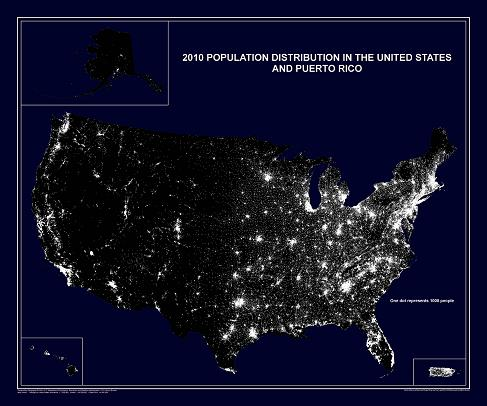
\includegraphics[width=\textwidth]{../figures/2010_census}
	\caption{Population density information for the U.S. and Puerto Rico from the U.S. census bureau \citep{2010_us_census}}
\end{figure}

We believe that the Universe began with a period of rapid inflation, and that in the process of this inflation, pockets of the Universe emerged more dense than other regions. This is revealed to us through observations of the cosmic microwave background (CMB). The CMB is a portrait of the Universe when it was last opaque; before electrons, neutrons, and protons combined to form the first atoms. It shows temperature fluctations, like small population overdensities, that would eventually become cosmic cities.  While many physicists marvel at the physics that happens in these first moments of time, the story of how galaxies grow from cosmic villages contains many puzzles. This is the story of how tiny perturbations evolve to the structures astronomers see today, and it starts with the CMB.

When we look at the CMB, we are seeing the temperature distribution of matter through the radiation of baryonic matter, the matter that interacts with light. There is strong observational evidence to suggest that a large fraction of the matter present at this epoch is not interacting with light, including the power spectrum of the CMB itself \citep{transfer_fn}. The power spectrum describes the distribution of scales of the perturbations in the CMB, and presents some of the strongest evidence for the existence of dark matter, matter which does not interact with light.

Not only is there a measurable dark matter component in the Universe, it appears to be substantial. If the results from the Planck satellite are taken as truth, then dark matter comprises around 84\% of all matter in the Universe \citet{planck_2018}. Dark matter influences the evolution of galaxies not only because it is not subject to radiation-based interactions, but also because it is most of what there is. Dark matter is the glue that holds galaxies together.  

If dark matter is a glue, then dark energy is the opposite. Although dark matter makes up 84\% of the matter, matter only makes up 31.5\% of the present day Universe. The remainder is composed by a small contribution from radiation, but the bulk is comprised of this unaccounted for dark energy \citep{kolb_turner,dodelson}. Dark energy, whatever it is, is likely responsible for the observation of accelerating Universe expansion from Type 1a supernova measurements \citep{reiss_1998,perlmutter_1999}. Modern cosmology is a struggle between the competing forces of dark matter and dark energy, and both have implications for the local dynamics in the Universe.

A model of the Universe one might consider is one comprised of cold dark matter, that is dark matter which is massive and slow, and one which has dark energy, described on large scales by a single parameter, $\Lambda$. This paradigm is called $\Lambda$CDM and is the prevailing model in the astronomy community. The model has been enormously successful in explaining observations, including the CMB power spectrum. While there remain open problems with $\Lambda$CDM, it appears to predict many properties on Galactic and extragalactic scales correctly \citep{kolb_turner,dodelson}. Proposals to modify $\Lambda$CDM tend to present only slight variations on the model, such as allowing for self interacting dark matter (SIDM).
\begin{figure}
	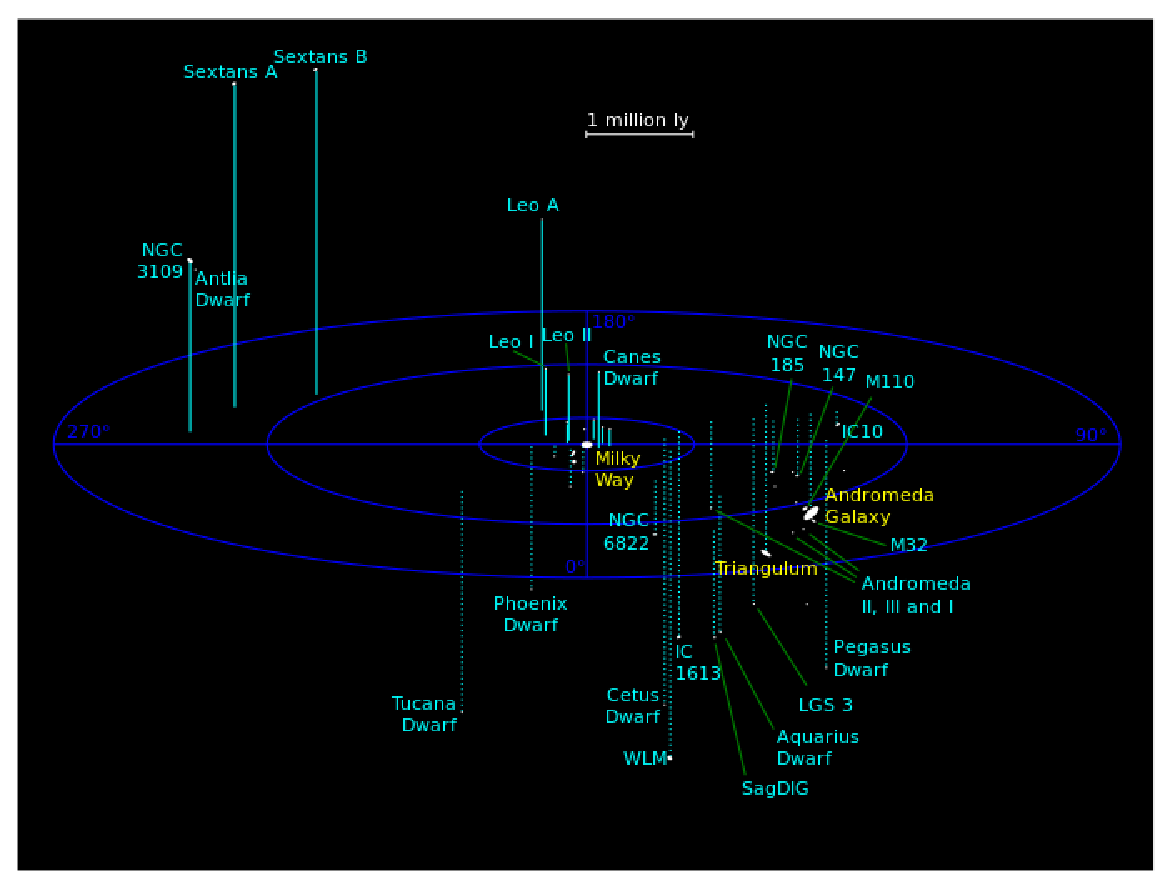
\includegraphics[width=\textwidth]{../figures/local_group}
	\caption{A map of the Local Group obtained per the license in \citet{local_group_map}.}\label{fig:local_group}
\end{figure}

Taking $\Lambda$CDM as the ground truth, the history of the Universe becomes understandable betweeen reionization and today. Dark matter, which does not interact through any force but gravity, retains a perturbed structure after inflation. The density perturbations collapse, forming potential wells of dark matter. The baryons, interacting through baryon acoustic oscillations (BOA), are delayed in falling into the potential wells made by the dark matter. As the baryons fall into the centers of the potential wells over time, the cores of the dark matter distributions, comprised of spheroidal units called halos, contract. After infall into a dark matter halo, the baryons cool to the point where stars are able to form. This is how the first galaxies formed.

Over time, galaxies begin to shift away from the linear mapping between perturbation and galaxy. Their forces on each other start to matter locally, and galaxies begin to merge hierarchically. Collections of galaxies form, sometimes massive clusters of $10^{15}$ solar masses. Other times, groups with a couple massive galaxies become host to many smaller galaxies called subhalos. Other galaxies belong to no group or cluster, and exist in the expansive void between clusters. Dark energy continues to pull the Universe apart, while locally galaxies are kept together by dark matter. Merging of galaxies continues on local scales as larger galaxies become larger, bringing us to today.

We live in a spiral galaxy of approximately $10^{12}$ solar masses (dark matter + baryons), in a group with another galaxy, M31 (Andromeda), which has a roughly similar mass. Our Local Group (Fig. \ref{fig:local_group}), as it is called, is comprised of many smaller galaxies. In our Milky Way's halo, for instance, a merger is beginning between the Milky Way and the Large and Small Magellanic Clouds (LMC/SMC), shown in the third quadrant of the inner circle around the Milky Way in Fig. \ref{fig:local_group}. The SMC/LMC systems total approximately 10-20\% of the Milky Way's mass in total \citep{erkal_lmc}. Most of our subhalos are not nearly this massive, although they number in the hundreds. The picture painted of the Local Group is that of M31 and the Milky Way devouring smaller galaxies. Of course, this will have a substantial impact on the evolution of the stars in the Milky Way, and is the crux of this thesis. By studying the Milky Way's local environment, we can hope to understand the interactions dark matter has on baryons, and perhaps infer something about how dark matter is distributed in our Galaxy.

%...the current de facto standard being the Unified Modeling Language
%(UML)~\cite{BRJ99}...

%\section{Problem}

%\section{Objective}

%\notesbox{Note:  These are the section headings that I decided to use.  Check out several
%recent theses to decide how you want to lay out your introduction (and conclusion) chapters.}


%\subsection{Hypothesis}

\section{Simulations as a Tool For Understanding Problems in $\Lambda$CDM}

Many of the hardest questions in Galactic astrophysics stem from the fact that dark matter is not directly observable. As an example, what is the underlying smooth distribution of dark mass? How many dark matter subhalos should the Milky Way have? What is the effect on large scales if we choose something other than $\Lambda$CDM? While these questions are not easily answerable by direct observation, we can complement indirect observations with a solid theoretical understanding to reach some confident answers.

Simulations are the complementary theoretical understanding of galactic and extragalactic systems. When a simulation is performed, theoretical input is considered. This includes your model of cosmology, or your model of the galaxy, the nature of dark matter, etc. All of this knowledge is reduced to a fluid system which may be solved through numerical techniques on a computer.  

Over the last four decades, many tools have been developed to study the structure of the present day Universe. These tools have become increasingly sophisticated as computation power and algorithms research advance. One tool is an \textit{ab initio} cosmological simulation, which simulates the entire formation history of the Universe from some informed initial density field.  This initial density field is derived from the primordial power spectrum, and a sample can be drawn and evolved with periodic boundary conditions \citep{music}. If done correctly, this creates a representative sample of many structures in a $\Lambda$CDM Universe. Halos evolving in these simulations feel the full effect of the completely simulated cosmological environment. Such simulations stand in contrast to isolated galaxy simulations, which seek to explain the detailed dynamics arising from generic effects in individual galaxies. These simulations start with a prescription for what an equilibrium galaxy looks like, and study the evolution of galaxies initialized from these prescriptions. While missing some critical cosmological physics, these simulations may be run at very high resolution.


When the results of a simulation are studied, we are studying the output of a given set of assumptions. In principle, this should allow us to evaluate whether or not cosmology is consistent with dynamics on a Galactic scale. $\Lambda$CDM has been tested in this way for decades, and we detail some global results in what follows. In particular, we focus on where simulations have shown discrepancies in cosmological theory.

We broadly commented on the hierarchical formation of galaxies. Over time, galaxies that merge with other galaxies should become well-mixed in the host halo. That is, there should be an underlying smooth distribution of mass in which all of the subhalos reside. A key prediction of $\Lambda$CDM is that this smooth distribution should have a universal density profile in the limit that dark matter dominates the Universe \citep{nfw}. Furthermore, the dark matter should have a density distribution somewhat resembling a squashed football, a spheroid flattened on two axes. Whether or not this picture holds observationally in real galaxies is an open problem. The density profile proposed by \citet{nfw} is cuspy at the center, whereas some observations are more consistent with a flatter central density \citep{de_blok_core_cusp}. Astronomers have dubbed this the Core-Cusp Problem. From simply running a dark matter only simulation, we can infer the relative significance that baryonic physics plays in the central part of galaxies from these observational inconsistencies.

Besides the Core-Cusp Problem in the inner parts of dark matter haloes, one thing that is clear is that $\Lambda$CDM halos should have many subhalos. As the general theory for the formation of galaxies goes, these subhalos were at one point independent perturbations that have since merged into the Milky Way's halo, and should have their own stellar and gas content. This means that we expect many massive subhalos to be directly observable. Another triumph of simulations is putting an actual number on how many subhalos we expect from $\Lambda$CDM. Surprisingly, far fewer subhalos are actually observed \citep{mooresubhalos, Klypin1999, springel2008}. This discrepancy has since been dubbed the Missing Satellite Problem, and is an open problem for $\Lambda$CDM and astronomy.


The Core-Cusp Problem and Missing Satellite Problem have received a lot of attention in the literature because of the potential problems they pose for theoretical cosmology. It is clear that to accurately recover the global properties of substructure on large scales, dark matter must be cold. Warm and hot dark matter models\footnote{Hot dark matter is comprised of matter moving at or near the speed of light (e.g. neutrinos), and warm dark matter is somewhere in between cold and hot dark matter.} simply do not yield substructure populations consistent with observations. SIDM and fuzzy models, where the dark matter can interact on small scales, have been proposed as slight modifications to the $\Lambda$CDM paradigm, with some success. Despite the presence of alternate theories of cosmology, a large concerted effort has been made to understand discrepancies as a byproduct of baryonic physics.  Adequeate explanation of halo and substructure response to stellar and gas content would mean that alternate cosmologies are not necessary to explain the Core-Cusp Problem and Missing Satellite Problem.


Initially, simulations included only dark matter, but have evolved over the last three decades to consider very sophisticated subgrid models of gas physics and star formation \citep{LucySPH,CenOstriker92,KatzSPH96,SpringelMultiphase03,Stinson2006}.  These simulations can be used to realize the galaxy formation predicted by current theories. State of the art unigrid (single resolution) cosmological simulations struggle to compete with the resolution attainable by isolated galaxy simulations \citep{Illustris,Eagle}, but they can still be used to make broad statements about consistency with $\Lambda$CDM. Broadly speaking, it is not clear at this stage whether or not apparent issues with $\Lambda$CDM can be resolved through these models, but they present a promising approach as computing power is sure to increase.

%Because of resolution factors, the goal of many of cosmology studies has shifted from studying galaxy dynamics to reproducing population statistics such as scaling relations.  As a consequence, problems which are at the interface of the complex cosmological environment and individual galaxy dynamics are still open.

All of the preceding is to say that simulations are an enormously valuable tool in understanding the broad predictions of cosmology on a Galactic scale. We have used them to uncover apparent inconsistencies in $\Lambda$CDM, and have a promising means within the paradigm to move forward in resolving these inconsistencies. All of the preceding discussion has focused on the complexity of the halo environment. Ultimately, we are looking for simulations to make observable predictions, and specifically signatures outside the Galactic halo that theory is correct.

\section{Dynamical Processes in a Chaotic Milky Way}

Up until this point, we have focused on the halo. This is the most massive component of our galaxy, holding a complicated geometry. The nature of this geometry is not directly probable, and we must rely on indirect methods to infer information about the halo. In addition to the dark matter halo, our Galaxy is composed primarily of a central spheroidal bulge, a thin disk, and a more diffuse thick disk. There is also a stellar component of the halo, which contains remnants of old mergers and star clusters known as globular clusters. This section is organized by talking about tidal disruption of subhalos in the Galactic halo, the dynamics of the central part of the Galaxy, and vertical structure in the Galactic disk. How the cosmological environment effects these observables is the bulk of this thesis, and we motivate here why these aspects are the subject of focus.

\subsection{Stellar Streams from Mergers}

In the hierarchical formation of galaxies, smaller galaxies merge with larger galaxies and become a part of the larger galaxy's halo. As subhalos become more a part of the host system, they experience tidal forces that stretch them apart. Dark matter and stellar material is stripped from these merging galaxies over time to form streams of tidal debris. In the long run, this debris will equlibrate with the stellar halo. It should be noted that the same effects apply to globular clusters too.

At the beginning of a merger event, the stellar debris left behind can detected. This is no easy task, and the first stream for which this accomplished was the debris of the Sagittarius Dwarf Spheroidal galaxy (Sgr dSph). The Sgr dSph was discovered by \citet{ibata_discovery}. The corresponding stream was later detected by \citet{newberg_2002} and \citet{majewski_2003}. 

These discoveries of debris associated with a merging dwarf galaxy kickstarted an onslaught of literature based on the detection of streams, and their potential uses in probing the Galactic potential. The general idea is that so long as streams approximately trace orbits in the halo, the correct Milky Way potential, dark matter and all, is the unique potential that reproduces these orbits. 

More streams have been discovered since then, and a few notable ones are the Orphan Stream \citep{grillmair_2006,belokurov_2007,newberg_2010}, remarkable for its apparent lack of progenitor, TriAnd, A13, and the Monoceros Ring. This is by no means a complete accounting of known stellar streams. Something on the order of more than a dozen streams are known to exist in the Milky Way alone \citep{sanders_binney_2013_a}. While streams alone have been useful in getting some broad contraints on the Galactic potential and geometry of the halo, complications arise from the fact that streams do not follow orbits exactly \citet{sanders_binney_2013_a} and the fact that the Milky Way potential is predicted from theory to be time dependent.

The orbits of streams are not the only way to learn about the Milky Way's dark matter halo. It is worth mentioning that there is the possibility of using the fine structure of stellar streams to learn more about the subhalo population in the halo.  Gaps form when subhalos pass through tidal streams, and this is one direction that is being explored for leveraging stellar stream data (e.g. \citet{erkal_2016_stream_gaps}).

%With the Sagittarius stream specifically, there 
\subsection{Response of the Galactic Disk to the Cosmological Environment}


We might also attempt to infer properties of the subhalo population through their effect on the Galactic disc.  It is believed that the affect of the Milky Way's substructure population can be observed as waves-like behaviour in the thin disc's vertical structure \citep{widrow_2012_sdss,carlin_2013_lamost, williams_2013_rave,xu_2015, carrillo_2018_rave}.  These waves can manifest as small corrugations in the Galactic disc, as global bending and breathing motions, or even as large warps in the Milky Way's gas  \citep{gasWarp} and stellar discs. It is worth noting that these observations are being confirmed in DR2 of the Gaia mission \citep[for example]{gaia_collab,bennet_2019_gaia}.

The Milky Way's massive subhalos are most likely inducing non-planar density patterns in the disc, and we would like to understand the nature of these patterns through simulation. Unfortunately, we need the high resolution of isolated galaxy simulations to study these effects, and the realism of an \textit{ab initio} Galactic halo.  This has motivated a long history of attempts to bridge the gap between {\it ab initio} cosmological simulations and those of isolated galaxies.  A particularly simple class of simulations involves the interaction of a disc
with a single satellite galaxy or dark matter subhalo.  For example \citet{kazantzidis2008} perform simulations in which a thin Milky Way-like disc is subjected to a series of encounters with a satellite.  The masses and orbital parameters of the satellites are motivated by substructure found in a halo appropriate to a Milky Way-like galaxy from a cosmological simulation.  Their simulation demonstrated that satellite encounters lead to general disc heating as well as distinctive disc features such as bars, spiral structure, flares, and rings.  \citet{purcell2011} model the response of the Milky Way to the gravitational effects of
the Sgr dSph by simulating disc-dwarf encounter for different choices of the Sgr progenitor's mass.  Their conclusion is that Sgr may have triggered the development the spiral structure seen today in the Milky Way.  This approach has gained considerable traction in the last couple years, with authors using single-satellite encounters to explain the existence of low-latitude streams and other vertical structure in the Milky Way's disc \citep[for example]{widrow_2014, dlv_2015, donghia_2016, laporte_2016, laporte_2018}. One particularly interesting feature arising from these works is that stars may occasionally be kicked out of the galactic disc to form kicked-up disc populations \citep{johnston_kud_review, laporte_2019_feathers}. Such populations may explain low-latitude Milky Way structures, and possibly kinematic data of M31 \citep{dorman_2013_m31}.

% Say something about KUD since you will focus on it. One interesting feature... Which might explain MW M31

Of course, the disc of the Milky Way lives within a population of satellite galaxies and, quite possibly, pure dark matter subhalos, and single-satellite encounters do not describe the complexity of the cosmological environment \citep{Klypin1999,mooresubhalos,springel2008}.  With this in mind \citet{Font2001} simulated the evolution of an isolated disc-bulge-halo model where the halo was populated by several hundred subhalos.  They concluded that that substructure played only a minor role in heating the disc, a result that would seem in conflict with those of the \citet{kazantzidis2008} that would come later.  Numerical simulations by \citet{gauthier2006, dubinski2008} sheds some light on this discrepancy.  In these simulations, 10\% of the the halo mass in an isolated disc-bulge-halo system is replaced by subhalos with a mass distribution motivated by the cosmological studies of \citet{gao2004}.  In the \citet{gauthier2006} simulation, little disc heating occurs during the first 5 Gyr, at which point satellite interactions provoke the formation of a strong bar, which in turn leads to significant heating.  Not surprisingly, when the experiment is repeated with different initial conditions for the satellites the timing of bar formation can vary.  These experiments also suggest that a large fraction of the mass initially in subhalos is tidally stripped leaving behind a complex system of tidal debris.

The aforementioned simulations, although more realistic than single-satellite encounters, have three main problems.  First, they don't allow for halo triaxiality.  Secondly, the disc is initialized at its present-day mass whereas real stellar discs form over several Gyr.  Finally, the subhalo populations are inserted into the halo by hand.  While the mass and spatial distributions of the subhalos are motivated by cosmological simulations, they may not capture important properties of realistic halos. This has historically been solved by modifying a traditional \textit{ab initio} simulation. The zoom-in technique (a Monte Carlo adaptive mesh) is used to study the evolution of a disc in a single halo at high resolution.  This is accomplished by resampling the initial conditions at a sequence of higher resolutions after identifying an area of interest. With sufficiently realistic feedback, impressively realistic results can be obtained. For instance, \citet{gomez_2017} presented a study of vertical structure in such simulations. While highly realistic, the \textit{ab initio} zoom-in approach still suffers from the inability to fine-tune galaxy dynamics in the same halo to perform a truly systematic study. In an effort to address these particular shortcomings, several groups have attempted to grow a stellar disc in a cosmological halo.  

\section{Bridging the Gap}


\section{Organization of Thesis}

We proceed by introducing conformance checking and discussing related work in the next
chapter. We discuss the Alloy language and the Alloy Analyzer tool in
Chapter~\ref{ch:Alloy}.  Chapter~\ref{ch:Embee1} describes our Embee tool, from the
user's perspective, with several running examples.  Implementation details and the
analysis of the tool are presented in Chapter~\ref{ch:Embee2}.
Chapter~\ref{ch:Conclusion} concludes and outlines future work.

\bibliographystyle{apalike}
\bibliography{bibliography_introduction}
\newcommand{\deriv}[3][]{% \deriv[<order>]{<func>}{<var>}
  \ensuremath{\frac{\partial^{#1} {#2}}{\partial {#3}^{#1}}}}
\newtheorem{theorem}{Theorem}[section]

\chapter{A Dynamical Recipe for Cosmological Disks}\label{ch:background}

This chapter provides an overview of the background theory needed to understand subsequent chapters. In Chapter~\ref{ch:introduction}, we had a lot of discussion about simulations of galaxies being critical to having a theoretical understanding of cosmology and galaxy formation. The word ``simulation" was used without fully contextualizing its significance and meaning. We provide that context in \S\ref{sec:motivation}, where we describe what is actually being done when a simulation is run. In \S\ref{sec:galaxy_ics}, we talk about how to apply this theory to study the evolution of equilibrium galaxies. We also spoke at length about $\Lambda$CDM cosmology and how it is critical to explain the evolution of galaxies on a global scale. We talk about cosmology in detail in \S\ref{sec:cosmology}, and explain how this specifies an extended view of the discussion in \S\ref{sec:motivation}. Lastly, we talk about various techniques relied upon in the analysis of simulation in \S\ref{sec:analysis_of_sims}. This includes how we identify cosmic substructure and the techniques we use for analyzing the time-evolution of disk-derived quantities. This chapter summarizes the very basics of the models used in this thesis. It is by no means a comprehensive account of galactic dynamics. In the course of discussion, we will point the reader to more detailed accounts of the topics being discussed.

\section{Physical Motivation of Modeling} \label{sec:motivation}

The goal of this section is to convey to the reader what we mean by a simulation of a galactic system. 

\subsection{Thermodynamics of Self-Gravitating Systems}

The baryonic mass of the Milky Way is largely concentrated in its stars. To first order, the dynamical behavior of the Milky Way is determined by stellar material and dark matter \citep{BM}. While the evolution of gas is governed by the Euler equations with an equation of state, modelling in galactic dynamics requires that we understand how stars and dark matter behave. 

We begin by suggesting a model of a galaxy composed only of a very large number of stars and dark matter, where all stars have the same mass. We call the probability of a star being a specific position, $\textbf{r}$, and velocity $\textbf{v}$, at a time, $t$, the distribution function (DF), $f(\textbf{r},\textbf{v},t)$. The stars and dark matter sit in a combined gravitational potential, $\Phi(\textbf{r})$, in some near-equilibrium state. To fully describe this model, we need to understand how an ensemble of self-gravitating particles gives rise to an equilibrium distribution of stars and dark matter.

Unlike gas, which can exhange thermodynamic energy with itself through a variety of mechanisms, stars and dark matter interact only through gravity. Gravity is a long range force. In fact, the majority of the contribution to the forces on stars in galaxies comes from far outside their immediate neighborhoods (that is to say gravitational energy in non-extensive) \citep{BT}. 

This has a number of interesting implications. Classical equilibrium statistical mechanics tries to understand distributions of particles as ensembles with a given thermodynamic potential. Some commonly used ensembles are the microcanonical ensemble, where $f_0(\textbf{r},\textbf{v})$, the equilibrium state, is determined by holding energy fixed in a closed system, and the canonical ensemble which finds $f_0$ holding the temperature of the system fixed \citep{sethna}. These ensembles break down when non-extensive forces are involed (in the latter case, specifically because self-gravitating systems have no maximum entropy) \citep{self_gravitating_statistical_mechanics,lb_negative_specific_heat, BT}. Another peculiarity of self-gravitating systems is that they have a negative heat capacity \citep{lb_negative_specific_heat}.

The implication is that self-gravitating systems of stars, which have no means to dissipate internal energy, can never be in thermodynamic equilibrium. A system which starts in dynamical equilibrium evolves to a state of higher entropy when perturbed, which is physically characterized as having a dense core and extended envelope of mass \citep{BT}. Since a thermodynamic resolution of why galaxies evolve the way the do is unattainable due to the extensive nature of gravity, we are forced to study non-equilibrium dynamical evolution of $f(\textbf{r},\textbf{v},t)$ to understand galactic systems, and this requires more theory\footnote{For more information on the thermodynamics of self-gravitating systems, Chapter~4.10 of \citet{BT} and Chapter~7.3 of \citet{BT} provide excellent summaries.}.

\subsection{The Collisionless Boltzmann Equation}

To provide a time-dependent dynamical prescription for our model of stars and dark matter particles, we will make a number of assumptions that hold for the entire thesis. These are:

\begin{itemize}
\item Galaxies are collisionless systems; one does not have to worry about energy exchanged in close encounters because close encounters of individual stars and dark matter particles seldom happen.
\item All stars and dark matter particles are identical.
\item Phase space probability is conserved.
\item Phase space probability is incompressible.
\end{itemize}
We want to turn the assumptions listed above into a solvable equation for $f(\textbf{r},\textbf{v},t)$. This is done by recognizing that  for $\textbf{w} = (\textbf{p}, \textbf{q})$ \citep{BT},
\begin{equation}
\deriv{f}{t} + \deriv{}{\textbf{w}} \cdot \left( f \dot{\textbf{w}}\right) = 0
\end{equation}
is the continuity equation in 6D phase space that expresses conserved phase space probability. Here, $\textbf{p}$ and $\textbf{q}$ are any set of canonical coordinates. In general, this may be rewritten in what is commonly called the Collisionless Boltzmann equation (CBE),
\begin{equation}
\deriv{f}{t} + \dot{\textbf{q}} \cdot \deriv{f}{q} + \dot{\textbf{p}} \cdot \deriv{f}{p} = 0.
\end{equation}
The CBE is more commonly expressed in Cartesian coordinates as,
\begin{equation}
\deriv{f}{t} + \textbf{v} \cdot \deriv{f}{\textbf{x}} - \deriv{\Phi}{\textbf{x}} \cdot \deriv{f}{\textbf{v}} = 0, \label{eq:cbe_cartesian}
\end{equation}
where $\Phi$ is our total gravitational potential from stars and dark matter. The result is a quasilinear partial differential equation (PDE) for $f(\textbf{r},\textbf{v},t)$. The CBE is nothing more than an advection equation in phase space that expresses our view that particles are not self interacting, that they are identical, and that the phase space fluid is conserved and incompressible. In addition to the CBE which describes the evolution of the phase fluid, we have the Poisson equation, an elliptic equation describing the evolution of the potential \citep{BT},
\begin{equation}
\nabla^2 \Phi(\textbf{r},t) = -4 \pi G \rho(\textbf{r},t) \label{eq:poisson}
\end{equation} 
where $G$ is Newton's gravitational constant and,
\begin{equation}
\rho(\textbf{r},t) = \int_{\mathcal{D}} f(\textbf{r}, \textbf{v}, t) \text{d}^3 \textbf{v},
\end{equation}
where $\mathcal{D}$ is the phase space. We are left with a 6D space + 1D time solution domain on which to compute $f(\textbf{r},\textbf{v},t)$ as well as two PDEs and an integral.

\subsection{Monte Carlo Solution of the Collisionless Boltzmann Equation}

In terms of actually solving the CBE, we run into a number of technical challenges in applying traditional finite difference and finite volume schemes for advection equations. These techniques require that some mesh be constructed, and the flows between the cells in the mesh are calculated dependent on the type of equation being solved and the current states of the cells\footnote{Chapter~19 of \citet{numerical_recipes_fortran} discusses numerical methods for PDEs, although you could find detailed discussion of finite difference and finite volume methods in most numerical methods texts.}. The spatial domain is 6D, meaning a uniform mesh resolution scales in memory consuption as $O(N^6)$, where $N$ is the number of cells on an axis. For a sanity check, a modest $N = 2^5$ element grid would take up $2^{30} \times 2^4 \text{ bytes} \sim 17 \text{ GB}$. We obviously need more than 32 cells on an axis to represent the fine DF structure we want to study, and we are already at the limit of a single compute node to apply a finite difference scheme. 

This is where Monte Carlo methods shine. The fundamental principle on which they operate is that I can evaluate the integral of any function, $f(\textbf{x})$, over a domain $\mathcal{D}$, as \citep{numerical_recipes_fortran},
\begin{equation}
\int_\mathcal{D} f(\textbf{x}) d^{n} \textbf{x} = \frac{V(\mathcal{D})}{\vert X_s \vert} \sum_{\textbf{x}_i \in X_s(\mathcal{D})} f(\textbf{x}_i)
\end{equation}
where $X_s$ is a uniform random sample of points on $\mathcal{D}$, $V(\mathcal{D})$ is the volume of the domain, $n$ is the dimensionality of $\textbf{x}$, and $\vert X_s \vert$ is the cardinality, or number of points in the sample. The benefit of Monte Carlo integration is that although our result is not deterministic, the error in the integral is reduced as $1/\sqrt{N}$ \textit{regardless of the integral's dimension}! 

The point of introducing this powerful concept is simply in recognition of the fact that we need to integrate over phase space to solve Eq. \eqref{eq:cbe_cartesian}. As we stated, computing these integrals on a mesh is intractible, so we represent $f(\textbf{r},\textbf{v},t)$ in another way:
\begin{equation}
f(\textbf{r},\textbf{v},t) \approx \sum_i m_i \delta^3(\textbf{r} - \textbf{r}_i) \delta^3(\textbf{v} - \textbf{v}_i)
\end{equation}
where $\delta^3$ is the 3D Dirac delta function, and we take the DF to be normalized to $M = \sum_i m_i$ instead of 1. We call this the N-body realization of the DF. As an extension of this idea, to find $f(\textbf{r},\textbf{v},t)$ at some point in the future, it is sufficient to find the state of our \textit{approximation}\footnote{The author believes that this is one of the most beautiful results ever to be applied in studying the dynamics of galaxies.} at some time in the future. This requires a more detailed exploration of how we step through time with N-body realizations.

\subsection{Time Integration in N-Body Simulations}

We have shown how to map solving the CBE, the master equation for our system of stars and dark matter, to the evolution of a finite sample of particles. The system of equations we need to solve now is,
\begin{eqnarray} \label{eq:nbody_system}
\dot{\textbf{r}}_i(t) &=& \textbf{v}_i(t)\\
\dot{\textbf{v}}_i(t) &=& -\left.\deriv{\Phi}{\textbf{r}}\right\vert_{\textbf{r} = \textbf{r}_i}.
\end{eqnarray}
Our integro-differential equation system is now approximated as $6\,N$, where $N$ is the number of particles sampled to represent the stars and dark matter, ordinary differential equations (ODEs). These may be solved by any ODE system solver. There are two competing objectives when deciding on the best way to handle time stepping numerically; the first is that we want to maximize the accuracy of our integration scheme and the second is that we want to minimize the number of evaluations of $-\nabla \Phi$, the force. The latter consideration is a severe constraint because naively, the complexity of evaluating each pairwise force is $O(N^2)$.  Although, as we will see, approximations reduce this complexity to $O(N\,\log \, N)$. We note that finding the forces amounts to solving \eqref{eq:poisson}.

Nonetheless, the force calculation will be the most time consuming aspect of the integration, and we want to minimize the number of evaluations we need. This rules out some commonly used schemes in the Runge-Kutta class of integrators, since they would require four or five calculations of the force on millions of particles \citep{numerical_recipes_fortran}. The open question is how to construct a low-order integration scheme that preserves the Hamiltonian\footnote{In a collisionless system, the Hamiltonian should be conserved \citep{BT}.}.

Define the following drift and kick operators for a forward timestep of $\Delta t$ as \citep{quinn_1997},
\begin{eqnarray}
D_t(\Delta t) : \begin{cases} 
	  \textbf{r}_i & \longrightarrow  \textbf{r}_i + \textbf{v}_i \Delta t\\
      \textbf{v}_i & \longrightarrow  \textbf{v}_i 
   \end{cases},
\end{eqnarray}
and,
\begin{eqnarray}
K_t(\Delta t) : \begin{cases} 
	  \textbf{r}_i & \longrightarrow  \textbf{r}_i\\
      \textbf{v}_i & \longrightarrow  \textbf{v}_i  - \nabla \Phi(\textbf{r}_i) \Delta T
   \end{cases}.
\end{eqnarray}
If the Hamiltonian is separable as $\mathcal{H} = T(v) + V(r)$ for $T$, the kinetic energy, and  $V$, the potential energy, and we are in a Cartesian coordinate system, combinations of these operators approximately preserve the Hamiltonian. This is a property of a class of integrators known as symplectic integrators, whose derivation starts with an assumption of Hamiltonian mechanics. We use the second order scheme implemented in \textsc{Gadget-3}, based on the code in \citet{GadgetCodePaper}. This integration scheme is specified as,
\begin{equation}
U(\Delta T) = K(\frac{\Delta t}{2}) D(\Delta t) K(\frac{\Delta t}{2}).
\end{equation}
This integration scheme is reasonably accurate with only two force evaluations, and is colloquially referred to as Leapfrog. It is also symplectic, meaning that the Hamiltonian of the system will not drift. Chapter~3 of \citet{BT} has an excellent comparison of numerical integrators, including the Leapfrog scheme given here.

The final remaining complication for the timestepping portion of solving the CBE is determining the timesteps themselves. This is slightly more complicated to do properly than choosing a fixed timestep for all particles. This is because accelerations and velocities in astrophysical systems vary by orders of magnitude, and the timestep needs to be small compared to the timescales defined by the relevant accelerations. The way that this is commonly implemented, including in \citet{GadgetCodePaper}, is to have a base timestep for all particles that gets bisected at each level of refinement. That is to say, particles at level 4 are updated four more times than particles at level 2. Suppose the highest level of refinement is $k$. The simulation proceeds in $\Delta t_{base} / 2^{k}$ intervals, with particles at $k - 1$ being updated at half of the timesteps, dividing the number of updates by two up to the coarsest level of temporal refinement. Where multiple levels need updates, particles at the lower levels are updated first.

The level of temporal refinement assigned to a given particle is determined primarily by the acceleration it experiences. That is, for \textsc{Gadget-3} \citep{GadgetCodePaper},
\begin{equation}
\Delta t_i = \min\left(\Delta t_{base}, \left(\frac{2 \eta \epsilon}{\vert \nabla \Phi(\textbf{r}_i) \vert} \right)^{1/2}\right).
\end{equation}
Here, $\eta$ is a free accuracy parameter and $\epsilon$ is the gravitational softening. The gravitational softening is used to prevent numerical overflow when particles rarely have close encounters. It arises from having the acceleration induced from a particle at position $\textbf{r}_i$  be,
\begin{equation}
\textbf{a}_i(\textbf{r}) = -\frac{G m_i}{\left(\vert\textbf{r} - \textbf{r}_i\vert^2 + \epsilon^2\right)^{3/2}}(\textbf{r} - \textbf{r}_i) \label{eq:point_mass}
\end{equation}
Higher choices of $\epsilon$ reduce large errors accumulating due to unsustainably large forces, but also make the force calculation less accurate.

\subsection{Efficient Force Calculation}

The Leapfrog scheme requires us to compute the force two times. Naively, we would compute a sum over Eq. \eqref{eq:point_mass} for each of the $N(N-1)/2$ unique pairs of positions in $O(N^2)$ time to compute the forces on all particles. This is also intractible, or rather is the limiting factor on how large of a simulation we can run. Methods were developed early on in the history of running N-body simulations to cope with this by approximating the potential.

The first method worth noting for this thesis is the particle mesh technique \citep{hockney_pm, white_pm, klypin_pm}. This technique considers the calculation of forces on a 3D mesh by reducing the calculation to a Fast Fourier Transform (FFT) \citep{numerical_recipes_fortran}. One of the crowning achievements of scientific computing in the 20th century was the rediscovery of an algorithm by J. W. Cooley and John Tukey, originally discovered by Gauss, to compute the discrete fourier transform (DFT) in $O(N\,\log\,N)$ complexity\footnote{What Gauss was doing with recursive DFT algorithms is beyond the author, but in the author's humble opinion, it is expected from the greatest mathematician to ever live.}\citep{fft}. Particle mesh's cloud-in-cell (CIC) algorithm was a part of a flurry of algorithms that subsequently exploited the FFT. It has a difficult time accounting for forces from particles separated by small scales on the mesh, though \citep{GadgetCodePaper}.

Compensating for some of the shortcomings of the particle mesh approach, \citet{barnes_hut} introduced a new algorithm for approximating forces in $O(N \,\log\, N)$ complexity. Their algorithm took a divide an conquer approach by subdividing the simulation space into octants recursively until each particle was in its own cell. Forces would be computed pairwise for particles close together, but for distant particles, the mass distrubtion would be approximated as a multipole. To compute the forces, one simply does a depth-first-search (DFS) of the particle tree, going deeper if,
\begin{equation}
\frac{l}{d} \geq \theta
\end{equation}
where $l$ is the side length of the node whose force is being computed, $d$ is the distance from this node to the current node in the DFS, and $\theta$ is a threshold called the opening angle. In the simplest case, a cell not meeting this condition would be approximated as a point mass with the position at the  center of mass of all particles deeper in its subtree. Higher order multipole expansions are typically used (4 and 8 are common choices).

In addition, the somewhat simplistic opening angle scheme is expounded upon by some codes to include a ``relative opening criterion". The main idea is to use the last acceleration of the particle to determine whether or not a cell needs to be opened. \textsc{Gadget-3} uses the criterion,
\begin{equation}
\frac{G M}{d^2} \left(\frac{l}{d}\right)^2 \geq \alpha \vert\textbf{a}_{i,t-1} \vert
\end{equation}
where $M$ is the mass in the current DFS subtree, $\vert\textbf{a}_{i,t-1} \vert$ is the magnitude of the acceleration of the current particle at the last time step, and $\alpha$ is a relative opening criterion, a free parameter. Conceptually, this means that if the point mass acceleration in the current subtree is greater than a specified fraction of this particle's acceleration, the current DFS level is too coarse and we need to go deeper.

The scheme proposed by \citet{barnes_hut} is widely used in astrophysics because of its efficiency and computability. While both algorithms are $O(N\,\log\, N)$ complexity, tree-based methods tend to perform more slowly in practice \citep{GadgetCodePaper}. \citet{xu_treepm} introduced a scheme to combine both the short-range accuracy of tree methods with the efficiency of FFT-based methods. This TreePM method has been widely successful at handling short range forces with a tree method and long range forces with particle mesh techniques. The trick is forcing consistency between the two methods at intermediate distances. \textsc{Gadget-3} combines a high degree of optimization with the TreePM algorithm to produce a highly efficient algorithm.

Before proceeding to talk about the complications of executing TreePM on distributed systems like the Linux clusters worked with in this thesis, we would be remiss in not mentioning field expansion methods. Typically these take the form of an expansion of the potential in spherical harmonics using a set of radial basis functions. A brief discussion of these methods is presented in Chapter~2.9.4 of \citet{BT}. These methdos have great historical significance, and have even seen a recent resurgence in helping understand the structure of dark matter halos \citep{lilley_2018_a, lilley_2018_b}.

To summarize, there are a number of ways to find gravitational forces in a simulation that all amount to solving Poisson's Equation, \eqref{eq:poisson}. The most accurate way is to compute all pairwise forces, but efficient algorithms have been developed to accurately estimate forces from gravity. The force calculation together with a timestepping scheme for N-body realizations forms the main components of an N-body simulation, and solving Eq. \eqref{eq:nbody_system} to estimate $f(\textbf{r},\textbf{v},t)$ is what we mean when we say we ran a simulation.

\subsection{Complications on Distributed Systems}

\begin{figure}
	\centering
	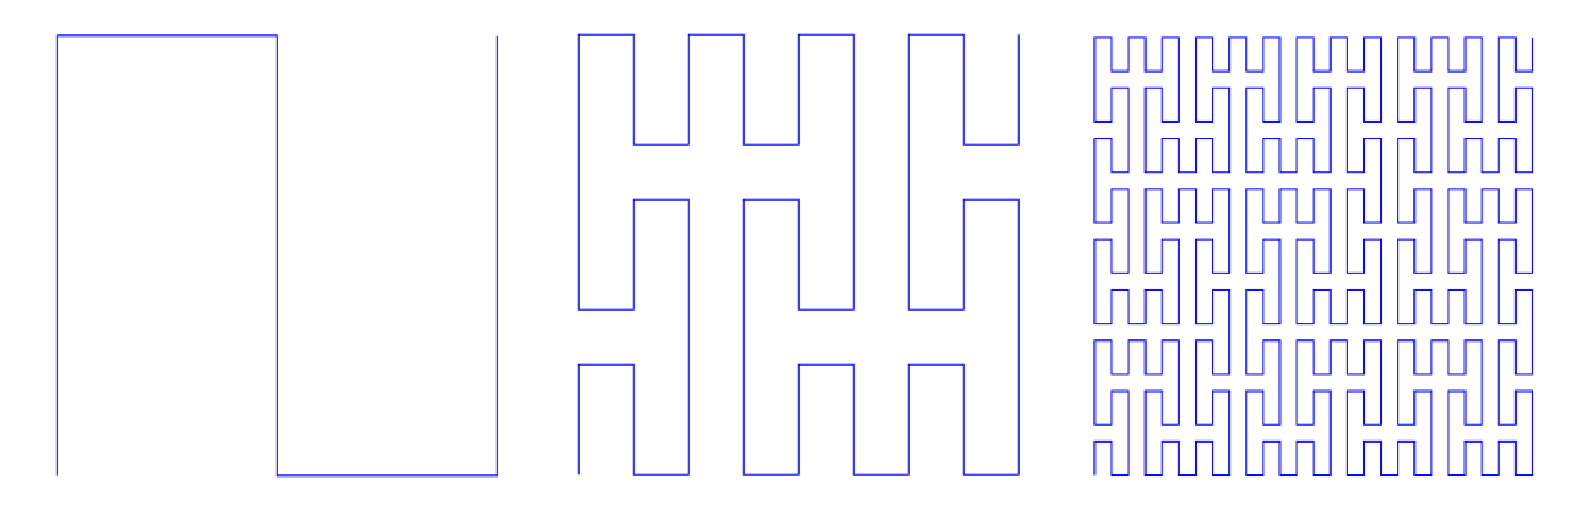
\includegraphics[width=\textwidth]{../figures/Peanocurve.eps}
	\caption{Several examples of the Peano space filling curve in 2D. The level of refinement increases left-to-right. Obtained from \citet{peano}.}\label{fig:peano}
\end{figure}

Modern high performance computing is largely done on compute clusters which are groups of smaller computers (nodes) connected with some high speed connection (Gigabit Ethernet, InfiniBand). The nodes form a distributed system in the sense that they do not share memory addresses. Each node may have multiple processes running (typically up to the number of logical cores on the node's CPU). Processes do not share data\footnote{Processes do not share data in a fully distributed model of parallel computing. Shared memory models like OpenMP \citep{openmp} share data between processes on a single node. MPI 3 even has similar shared memory support \citep{mpi3_shared}. \textsc{Gadget-3} was initially designed to not use these paradigms, and our intention is not to give a complete overview of all of parallel computing, so we relegate clarification to this footnote and references.}, and must communicate through a protocol like the Message Passing Interface (MPI) \citep{mpi_standard}.

Specifically, in an N-body simulation,  will have a subset of all of the particles, and a subset of the total tree structure. A naive DFS of an Octree simply cannot be done since no process will have all of the particles. When a process requires particles from another process, this reduces the efficiency gained from increasing the number of processors, and one might even get an overall slowdown. Another potential problem is that an individual process may get a higher work load than other processes, causing the other processes to wait for it to finish. We talk about how both of these problems are solved here.

To reduce the need to explicitly transfer particles between processes, \textsc{Gadget-3} notes that pairwise forces will only be needed for nearby poarticles. These represent the bulk of the tree force calculation. Any scheme which puts nearby particles on the same processor will reduce the overall communication time in the force calculation phase. One way to accomplish efficient load balancing is to partition the simulation space using a space filling curve. Fig. \ref{fig:peano} shows the Peano space-filling curve at several levels of refinement in 2D. This is the curve \textsc{Gadget-3} uses. A level of refinement is selected, and estimates of the computational cost in each cube are added up along the space filling curve to equally distribute the computational load. This results in nearby particles being on the same process, and in the processes having roughly equal work loads. \citet{GadgetCodePaper} shows that this is highly effective at reducing communication cost in the simulation, and it goes into more detail about how TreePM is carried out on distributed systems.


\section{Phase Space, Equilibrium, and Initial Conditions} \label{sec:galaxy_ics}
In \S\ref{sec:motivation} we outlined the underlying theory behind representing stars and dark matter in an N-body simulation. The focus of this thesis is studying the behavior of stellar disks in cosmological environments, and the first step towards that understanding is the construction of a pristine, equilibrium N-body model. Ultimately, in the course of running an N-body simulation, these pristine systems will diverge to higher entropy states, initially due to random errors in the N-body representation. Nonetheless, these models give us an understanding of how perfectly unperturbed galaxies will evolve due to the fact that real galaxies are also made of a finite number of particles.

\subsection{Jeans Modeling and the Epicyclic Approximation}

The DF represents the 6D phase space information and completely describes an N-body system. In a simple disk-halo system, there is a flattened axisymmetric component (the disk), and a spheroidal component (the dark matter halo) each with their own DF. These are made self-consistent by the separate DFs' incorporation of their combined gravitational potential. 

However, the DF is not the quantity that is observed in external galaxies. Astronomers are not typically working with a 6D phase space description of the structures they observe. Luminosity (density) profiles are one observable , as well as circular velocities (rotation curves) for disks, and also the spread of line of sight (LOS) velocties of disk stars. A modelling approach that takes our understanding of these observables as input is conceptually easier to understand than a DF which may or may not be unique \citep{BT}.

In this spirit, \citet{jeans_1915}\footnote{Notably before the infamous 1920 Curtis-Shapley debate \citep{curtis_shapley} establishing that so-called ``spiral nebulae" were actually external galaxies.} laid out a framework to describe galaxy evolution in terms of the \textit{moments} of the distribution function. Specifically, the idea is to multiply the CBE (Eq. \eqref{eq:cbe_cartesian}) by $\textbf{v}_i$ or $\textbf{v}_i \textbf{v}_j$ and integrate over the velocity part of phase space. These together yield the second-order Jeans equations \citep{BT},
\begin{eqnarray}
\deriv{\nu}{t} + \deriv{\nu \langle v_i \rangle}{x_i} &=& 0 \\
\nu \deriv{\langle v_j \rangle}{t} + \nu \langle v_i \rangle \deriv{\langle v_j \rangle}{x_i} &=& -\nu \deriv{\Phi}{x_j} - \deriv{\nu \sigma^2_{ij}}{x_i}\label{eq:jeans}
\end{eqnarray}
where $i,j \in (1,2,3)$, $\langle\cdot\rangle$ denotes expectation over $f$, $\mathbb{E}_f[\cdot]$, $\nu$ is the number density of particles, and $\sigma^2_{ij} = \langle v_i v_j \rangle - \langle v_i \rangle \langle v_j \rangle$ is the velocity dispersion tensor. In equilibrium for spherical systems, the second equation is often written as \citep{BT},
\begin{equation}
\deriv{\nu \langle v_r^2 \rangle}{r} + \nu \left(\deriv{\Phi}{r} + \frac{2 \langle v_r^2 \rangle - \langle v_\theta^2\rangle - \langle v_\phi^2 \rangle}{r} \right)
\end{equation}
where $\theta$ is the polar angle, $\phi$ is the azimuthal angle, and $r$ is the spherical radius\footnote{Note a slight abuse of notation. We said that $v_i$ has $i \in (1,2,3)$, but here we use symbols to represent specific coordinate systems. The point is that the indices have three unique values.}. Note that there is only one scalar equation. Symmetries in the velocity dispersion tensor for spherical systems require that the cross moments are zero \citep{BT}. For axisymmetric systems, the equilibrium Jeans equations are often written \citep{BT},
\begin{eqnarray}
\deriv{\nu \langle v_R^2 \rangle}{R} + \deriv{\nu \langle v_R v_z \rangle}{z} + \nu \left(\frac{\langle v_R^2 \rangle - \langle v_\phi^2 \rangle}{R} + \deriv{\Phi}{R} \right) &=& 0\\
\frac{1}{R} \deriv{R \nu \langle v_R v_z \rangle}{R} + \deriv{\nu \langle v_z^2 \rangle}{z}+ \nu \deriv{\Phi}{z} &=& 0\\
\frac{1}{R^2} \deriv{R^2 \nu \langle v_R v_\phi \rangle}{R} + \deriv{\nu \langle v_z v_\phi\rangle}{z} &=& 0
\end{eqnarray}
where $z$ is the Cartesian $z$, $R$ is the cylindrical radius, and $\phi$ is the polar angle. These equations look suspiciously like Euler's equations for fluid dynamics with a missing energy equation. \citet{jeans_1915} did not magically solve the statistical mechanical issues mentioned in \S\ref{sec:motivation}; given a number density and potential, we still have an unknown velocity dispersion tensor with six elements, and only 4 independent equations. In the simplified spherical case, we have three unknown elements and two independent equations.

We have also thrown out information about the DF by using moments and stopping at second order. Higher order Jeans equations can be appended to this system by multiplying the CBE by $v_i v_j v_k$ to obtain the third order equations, and so on. These get progressively more complicated, and we would require more additional equations to evaluate the equilibrium Jeans equations \citep{BT}.

Despite these shortcomings, more information can be imposed on the system to make these equations applicable. \citet{hernquist_1993} was one of the first successful applications of Jeans modelling to creating equilibrium galaxies with bulges, disks, and dark matter halos. In the case of the dark matter halo for a disk-halo system, one only has to specify the function,
\begin{equation}
\beta(r) = 1 - \frac{\langle v_\theta^2\rangle + \langle v_\phi^2 \rangle}{2 \langle v_R^2 \rangle}.
\end{equation}
This parameter measures anisotropy in the velocity ellipsoid defined by $\sigma_{ij}$ at each radius; $\beta = -\infty$ if all orbits are circular, $\beta=0$ if the system is isotropic, and $\beta = 1$ if orbits are purely radial. Together with an assumed density-potential pair, continuity equation, and the spherical second-order Jeans equation, the spherical halo's velocity structure is specified. At the time of writing, \citet{hernquist_1993} did not have much information about the dark matter distribution in galaxies (recall \citep{nfw} proceeded this work in establishing a common density profile for dark matter halos). As such, we will not talk about their uninformed choice of halo, and it really is not important.

In the case of the axisymmetric disk, \citet{hernquist_1993} based their model on the observations at the time which suggested that stellar disks had an exponential radial density profile \citep{freeman_1970}. This motivated a density profile commonly used today,
\begin{equation}
\rho_d(r) = \frac{M_d}{4 \pi R_d^2 z_d} e^{-R/R_d} \text{sech}^2\left(\frac{z}{z_d} \right). 
\end{equation}
Here, $M_d$ is the mass of the disk, $R_d$ is the radial scale length, and $z_d$ is the vertical scale length.
Observations support the idea that the second radial velocity moment also has an exponential profile \citep{van_der_kruit_searle_1981, lewis_freeman_1989},
\begin{equation}
\langle v_R^2  = \sigma_{R,0} e^{-R/R_\sigma}.
\end{equation}
Here, $R_\sigma$ is the radial dispersion scale length, and $\sigma_{R,0}$ is a free velocity scale (on the order of 100 km/s for the Milky Way). In  priciple, any radial scale length can be used for $\langle v_R^2 \rangle$, but it is generally accepted to be a longer scale length than $R_d$. The vertical dispersion and second velocity moment are determined from the assumption of the disc being isothermal,
\begin{equation}
\langle v_z^2 \rangle = \pi G \Sigma z_d
\end{equation}
where $\Sigma_d$ is the surface density as a function of radius. Finally, a relation between $\langle v_\phi^2 \rangle$ and the other second moments is needed to fully solve the second order system. Jeans modelling for discs injects the intuition behind a theoretical development known as the \textit{epicycle approximation}. 

The main idea is that stars in discs are on roughly circular and planar orbits, so a reasonably accurate description of their orbits can be obtained by taking the equations of motion in a truncated series expansion about a circular orbit at the guiding radius, $R_g$. This is better understood in terms of the effective potential in the rotating reference frame in which a star rotating at $R_g$ is stationary. For a star on the $x$-axis, the $\hat{x}$ direction represents the radial direction, the $\hat{y}$ direction is the same as $\hat{\phi}$ in the original frame, and $\hat{z}$ is unchanged. The equations of motion are \citep{BT},
\begin{eqnarray}
\frac{\text{d}^2x}{\text{d} t^2} &=& \deriv{\Phi_{eff}}{R}\\
\frac{\text{d}^2y}{\text{d} t^2} &=& 0\\
\frac{\text{d}^2z}{\text{d} t^2} &=& \deriv{\Phi_{eff}}{z}
\end{eqnarray}
where $\Phi_{eff} = \Phi(R,z) + L_z^2/2 R^2$ is the efffective potential in the accelerating (rotating) reference frame, and $L_z$ is the $z$-component of the angular momentum. These equations can be written in a first order expansion as,
\begin{eqnarray}
\frac{\text{d}^2x}{\text{d} t^2} &=& \kappa^2 x\\
\frac{\text{d}^2y}{\text{d} t^2} &=& 0\\
\frac{\text{d}^2z}{\text{d} t^2} &=& \nu^2 z
\end{eqnarray}
where,
\begin{equation}
\kappa^2(R_g) = \left(R \deriv{\Omega^2}{R} + 4 \Omega^2\right)_{R=R_g,z=0},
\end{equation}
with the circular frequency $\Omega$,
\begin{equation}
\Omega^2(R_g) = \frac{1}{R_g} \left(\deriv{\Phi}{R}\right)_{R=R_g,z=0} = \frac{L_z^2}{R_g^4},
\end{equation}
and,
\begin{equation}
\nu^2(R_g) = \left(\deriv{\Phi}{z}\right)_{R=R_g,z=0}.
\end{equation}
That is, a star's orbit is decribed by three frequencies: its rotational frequency $\Omega$, a radial oscillation frequency, $\kappa$, and a vertical oscillation frequency, $\nu$. This view is accurate so long as the vertical motion does not deviate far from the disc midplane. The actual values of these constants in Galactic astonomy are related to a problem known as the \textit{Oort Problem}, and we believe that for the Sun \citep{BT},
\begin{eqnarray}
\frac{\kappa}{\Omega} &\approx& 1.35 \\
\frac{\nu}{\kappa} &\approx& 2
\end{eqnarray} 
The fact that the orbit is described by three distinct frequencies that are unequal for the Sun means that the Sun's orbit does not close. If the Milky Way potential never changed, the path of the Sun would fill an annulus centered around $R_g$ \citep{BT}. That is to say, the orbit looks like it forms a rosette pattern.

By assuming the epicycle approximation, we are able to form a complete solution to the Jeans equations for the disc. This is done by looking at a dynamical property of disc star orbits called \textit{asymmetric drift}, which is the velocity defined by \citep{BT},
\begin{equation}
v_a = v_c -  \langle v_\phi \rangle
\end{equation}
where $v_c = R \Omega$. We have yet to discuss how we find $\langle v_\phi^2 \rangle$, whose non-zero nature explains why we have asymmetric drift in the first place. By evaluating the asymmetric drift with the assumptions of the epicycle approximation, we get \citep{hernquist_1993},
\begin{equation}
\sigma_\phi^2 = \langle v_\phi^2 \rangle = \langle v_R^2 \rangle \frac{\kappa^2}{4 \Omega^2},
\end{equation}
where the fraction in the product contains quantities solely determined from the potential, and the coefficient is determined from the assumed radial dispersion profile. This fully solves a disc-halo system. In practice, the system is realized by sampling the spatial density profile (by rejection sampling, for instance) and assigning velocities assuming Gaussians with means $\langle v_i \rangle$ and variances $\langle v_i^2 \rangle$. 

\subsection{DF-based Models and the Jeans Theorem}

Although Jeans modeling is used to set up initial conditions for galaxies because it does not require a DF to be known ahead of time, the best initial conditions are generated from DFs \footnote{That is not to say that no one uses Jeans modelling to set up ICs. Approaches like the one presented in \citet{hernquist_1993} were enormously successful and still used today.}. In general, the equilibrium DF is a function of six variables. However, there are some quantities, called \textit{integrals of motion}, which do not change along a star's orbit in a potential. For an axisymmetric potential, these are the total energy, $\mathcal{E}$, $L_z$ and a third quantity, $I_3$.  
For spherical systems, up to five integrals of motion are admitted by the system, but the simplest \textit{ergodic} models simply have $f_{h}(\mathcal{E})$ for the DF. 


If we assume the epicycle approximation, then $I_3 \approx E_z = \Phi(R,0) - \Phi(R,z) + \frac{1}{2} v^2$, where $v$ is the velocity of an orbit \citep{kd95galactics}. The vertical energy, $E_z$, is conserved so long as the disc is razor thin. Jeans showed that a DF that is a function of the integrals of motion describes an equilibrium distribution. More specifically, quoting from \citet{BT},
\begin{theorem}[The Jeans Theorem]
Any steady-state solution of the collisionless Boltzmann equation depends on the phase-space coordinates only through integrals of motion in a givcen potential, and any function of the integrals yields a steady-state solution of the collisionless Boltzmann equation.
\end{theorem}
Proof of this theorem can be obtained in \citet{jeans_1915} and in Chapter~4.2 of \citet{BT}, although it essentially amounts to observing that the time derivative of a function of time-independent quantities is zero by the chain rule. Now that we know that any DF of the intergrals of motion gives a steady state solution, and that using the epicyclic approximation gives us three known integrals of motion, we can ask ourselves what kinds of DFs describe the NFW haloes and exponential disks that are easily obtained from Jeans modelling.

We talk about the case of an ergodic halo and DF yielding an exponential disc at length here. For the remainder of the thesis, we primarily generate our initial conditions in this way. For any ergodic DF, a chosen density profile may be inverted by the Eddington inversion formula \citep{BT},
\begin{equation}
f(\mathcal{E}) = \int_0^{\mathcal{E}} \frac{\text{d} \Psi}{\sqrt{\mathcal{E} - \Psi}} \frac{\text{d} \nu}{\text{d} \Psi} \label{eq:eddington}
\end{equation}
where $\Psi = - \Phi$. Note that the combined potential need not be spherical, only the overall density of the spheroidal halo. We choose a truncated NFW profile \citep{nfw},
\begin{equation}
\nu_h(r) \sim \rho_{h}(r) = \frac{\rho_0 R_s^3}{r (R_s + r)^2}
\end{equation}
where $\rho_0$ is a scale density and $R_s$ is the halo scale length as our target halo denity. By obtaining the 1D DF from Eq. \eqref{eq:eddington}, we can sample halo orbits given the combined disc-halo potential.

For the disc DF, we use a DF that yields exponential discs presented in \citet{kd95galactics}. Noting that if $E_z$ is an integral of motion that $E_p = \mathcal{E} - E_z$ is also an integral of motion, we use,
\begin{equation}
f_d(E_p,L_z,E_z) = \frac{\Omega(R_c)}{(2 \pi^3)^{1/2} \kappa(R_c)} \frac{\tilde{\rho_d}}{\tilde{\sigma_R}^2(R_c) \tilde{\sigma_z}(R_c)} \exp\left[-\frac{E_p - E_c(R_c)}{\tilde{\sigma_R}^2(R_c)}  - \frac{E_z}{\tilde{\sigma_z}^2(R_c)}\right].
\end{equation}
Note that the quantities $\Omega$ and $\kappa$ have their usual definitions, the tilde functions are free choices to tune the disc properties (although they are qualitaively understood as velocity dispersions), and $E_c$ is the energy of a circular orbit. Note that the $R_c$-dependent quantities do not violate the sole dependence on integrals of motion, since $R_c$ is uniquely obtained in a one-to-one fashion from $L_z$.

In terms of the choices for the tilde functions, we choose them to yield the closest thing to an exponential-sech$^2$ density profile with and exponential radial velocity dispersion as possible. Assuming an exponential radial dispersion profile, a disc density is obtained by iteratively adjusting $\tilde{\sigma_z}$ and $\tilde{\rho}$ such that \citep{kd95galactics},
\begin{equation}
\rho_d(R,z) = \frac{M_d}{8 \pi R_d^2 z_d} e^{-R/R_d} \text{erfc }\left(\frac{R - R_{out}}{\sqrt{2} \delta R_{out}}\right) \exp \left[ -0.8676 \frac{\Psi_z(R,z)}{\Psi_z(R,z_d)}\right]
\end{equation}
Here, $M_d$ is a parameter that is approximately equal to the mass of the disk, $R_{out}$ is a truncation radius, $\delta R_{out}$ is a parameter determining the sharpness of the truncation, and $\Psi_z$ is the negative vertical potential, $\Phi(R,0) - \Phi(R,z)$. The motivation behind the last term in the product is to yield a dropoff of vertical density close to $\text{sech}^2(z/z_d)$.

Similar to the  Jeans models, we actualize these systems by sampling their combined spatial densities. At every sampled point, we draw a velocity from the DF that is constructed in the combiend potential. This does not require us to, for example, use a Gaussian distribution for the velocity dispersions as in Jeans models. This kind of model is as accurate as the assumption that $E_z$ is an integral of motion is (as accurate as the epicycle approximation is). A more detailed discussion about how self-consistent systems are realized from DFs can be found in \citet{kd95galactics}, and this work forms the basis for the \textsc{GalactICS} code used in this thesis.

\subsection{Action-Angle Variables and the Strong Jeans Theorem}

Of course, $E_z$ is only approximately an integral of motion for axisymmetric, nearly planar systems. Although not a substantial element of this thesis, it is worth mentioning a different approach to approximating integrals of motion. Instead of explicitly assuming we are working with an axisymmetric, static system and deducing the conserved quantities, let's ask more generally, \textit{for any system}, what are the conserved quantities? Integrals of motion have the property that orbits may be viewed as single points in a space with dimension of the number of integrals. The only thing unique about them is where they are in the phase of the orbit.

With this in mind, we introduce the actions \citep{BT},
\begin{equation}
\textbf{J} = \oint \textbf{p} \cdot \text{d}^n \textbf{q}
\end{equation}
where $\textbf{J}$ are the actions, and $textbf{p}$ and $\textbf{q}$ are canonical coordinates. The closed path over which this integral is evaluated yields a unique set of actions. If the system is axisymmetric and the path we have chosen is a circle of radius $R$, it is straightforward to see that the radial component of the action is just $L_z = R v_c$, which depends on the potential. 

Turning the definition of the actions into a transformation from a physically motivated conjugate coordinate system is difficult in general. Closed form solutions for axisymmetric systems exist if the potential if of the St\"ackel form\footnote{For more detail, see Chapter~3.5.3 of \citet{BT}.}, but in general, these transformations do not exist. A commonly used technique is to locally approximate the potential as being of the St\"ackel form \citet{binney_2012}. In practice, one is reduced to approximating the potential instead of the third integral of motion as in the case of \textsc{GalactICS}. For nearly planar disc systems, the differences are insignificant, but become more relevant as one wants to initialize a thicker disc \citep{vasiliev_2018,bauer2018b}.


\section{Cosmology and Implications for Galaxy Studies} \label{sec:cosmology}
Our discussion up to this point has focused on simulating isolated systems. Complications arise when we move to a fully cosmological environment. The purpose of this section is to briefly review relevant cosmology, and to explain what numerical methods must be modified and used to simulate cosmological systems. We conclude this section with a brief commentary on identifying substructure in simulations.

\subsection{Simulations of FRW Cosmology: Large Scale Properties}

In words, the $\Lambda$CDM paradigm described in Chapter~\ref{ch:introduction} prescribes a Universe comprised of four fundamental substances: baryond, radiation, dark matter, and dark energy. On large scales, the Universe is also believed to be isotropic and homogeneous, meaning the patch we occupy is the exact same as any other patch. General Relativity provides a mechanism for us to meaningfully compute distances between patches is this scenario. The so-called Friedmann-Robertson-Walker metric tells us that the \textit{proper distance} between two points at different positions in space and at different times is \citep{kolb_turner, dodelson},
\begin{equation}
\text{d}\,s^2 = c^2 \text{d}\,t^2 + a^2(t) \left(\frac{\text{d}\,r^2}{1 - k r^2} + r^2\text{d}\,\Omega^2 \right).
\end{equation}
Here, $c$ is the speed of light, $t$ is the time coordinate, $a$ is the scale factor of the Universe which is equal to 1 at present day and 0 at the Big Bang, $k$ describes the spatial curvature, and $r$ and $\Omega$ have their standard spherical coordinate definitions. The case used for the whole thesis is where $k=0$, a flat Universe. Assuming this metric, and that all substances in the Universe behave like perfect fluids, it can be shown with General Relativity that the large scale evolution of the Universe is described by the following, the Friedmann Equations \citep{kolb_turner,dodelson},
\begin{eqnarray}
\left( \frac{\dot{a}}{a} \right)^2 &=& \frac{8 \pi G}{3} \rho\\
\frac{\ddot{a}}{a} &=& -\frac{4 \pi G}{3}\left(\rho + \frac{3 p}{c^2}\right).
\end{eqnarray}
Here $\rho$ is the density of the Universe, $p$ is the pressure of the Universe, and we introduce the defintion $H(t) = \dot{a} / a$, the Hubble parameter. With the definition of the Hubble parameter, the first of the Friedmann equations is commonly expressed,
\begin{equation}
\left(\frac{H(t)}{H_0}\right)^2 = a^{-4} \Omega_{R,0} + a^{-3} \Omega_{M,0} + \Omega_{\Lambda,0}
\end{equation}
where $\Omega_{R,0}$, $\Omega_{M,0}$, and $\Omega_{\Lambda,0}$ are the relative contributions of radiation, dark and baryonic matter, and dark energy at present day, respectively. Also, $H_0$ is the present-day Hubble parameter. Every flat $\Lambda$CDM universe has these as free parameters, and we can choose them to be anything we like. The different powers of $a$ reflect how radiation, matter, and dark energy contribute differently to the energy as the Universe expands, and can be deduced under relatively few assumptions \citep{kolb_turner,dodelson}.

When simulating a $\Lambda$CDM universe, we can choose to work in a frame where relative distances between fixed points remain fixed.

% Comoving coordinates


\subsection{Simulations of FRW Cosmology: Cosmological Initial Conditions}

Of course, the Universe is not actually homogeneous on small scales. As we suggested in Chapter~\ref{ch:introduction}, small scale fluctuations are present in the early Universe which collapse to form galaxies. Initially, these fluctuations evolve independently of each other in the so-called \textit{linear regime}. Initial conditions for $\Lambda$CDM simulations rely on this fact to generate the initial perturbations for the simulation.

The prevailing view in cosmology is that the Big Bang was followed by the development of a primordial perturbation field. As the Universe expanded, interactions with baryons and radiation modified the initial distribution of perturbation scales. Mathematically, we take the the perturbation field $\delta(\textbf{r}, t)$, which describes the deviation from the Universe's mean density at some position and time, and find its Fourier transform. The result is a statistical distribution, called the \textit{power spectrum}, that describes the scale of perturbations \citep{music},
\begin{equation}
P(k) = \alpha k^{n_s} \mathcal{T}^2(k)
\end{equation}
where $\alpha$ is a normalization constant, $n_s$ is a spectral index describing the original inflationary produced perturbations, and $\mathcal{T}$ is a scale-dependent \textit{transfer function} that describes deviations from a power law at different scales. For reference, low $k$ corresponds to larger perturbations in the same way that low frequency corresponds to larger time gaps. The smallest structures occur at high $k$.  

While a detailed discussion of how the transfer function is computed can be found in \citet{music}, we will simply say that it is a reflection of the idea that perturbations only grow when matter becomes dominant. It reflects how we believe that perturbations of different scales grew at different rates in the early Universe. However, once it is known at some desired time (redshift), we can sample a Gaussian density field with the right statistical characteristics. This spatial sample with corresponding velocities obtained via something called 2nd Order Lagrangian Perturbation Theory\footnote{See \citet{music} for a detailed description of this technique.} form the initial conditions for our $\Lambda$CDM simulation.

% Maybe say something about zoom-ins?
\subsection{Extension of Numerical Methods: Time Integration}

Two big problems are present for applying N-body techniques as described. The first, and maybe most obvious of these, is in how we 

\subsection{Extension of Numerical Methods: Gravity Calculation}

\subsection{Identifying Substructure in Simulations}


%\section{Simulation Analysis: Paradigms and Tools} \label{sec:analysis_of_sims}
%\subsection{Cosmological Substructure and Halo Triaxiality}
%\subsection{Identifying Substructure in Simulations}
%\subsection{WKB Wave Analysis}
%\subsection{Time Series Filtering}
%\subsection{MCMC}
\bibliographystyle{apalike}
\bibliography{bibliography_background}



\chapter{A Method for Studying Discs in Cosmological Haloes} \label{ch:paper_i}
\textbf{This chapter contains a reproduction of a paper published in  Monthly Notices of the
Royal Astronomical Society as: Jacob S. Bauer, Lawrence M. Widrow, and Denis Erkal. Disc-halo interactions in $\Lambda$CDM. \textit{Monthly Notices of the Royal Astronomical Society}, 476:198-209,
2018.}
\newpage
\section{Abstract}

We present a new method for embedding a stellar disc in a
cosmological dark matter halo and provide a worked example from a
$\Lambda$CDM zoom-in simulation.  The disc is inserted into the halo
at a redshift $z=3$ as a zero-mass rigid body.  Its mass and size
are then increased adiabatically while its position, velocity, and
orientation are determined from rigid-body dynamics.  At $z=1$,
the rigid disc is replaced by an N-body disc whose particles sample
a three-integral distribution function (DF).  The simulation then
proceeds to $z=0$ with live disc and halo particles.  By comparison,
other methods assume one or more of the following: the
centre of the rigid disc during the growth phase is pinned to the
minimum of the halo potential,  the orientation of the rigid disc is
fixed,  or the live N-body disc is constructed from a two rather than
three-integral DF.  In general, the presence of a disc makes the halo
rounder, more centrally concentrated, and smoother, especially in
the innermost regions.  We find that methods in which the disc is
pinned to the minimum of the halo potential tend to overestimate the
amount of adiabatic contraction.  Additionally, the effect of
the disc on the subhalo distribution appears to be rather insensitive
to the disc insertion method.  The live disc in our simulation
develops a bar that is consistent with the bars seen in late-type
spiral galaxies. In addition, particles from the disc are
launched or ``kicked up'' to high galactic latitudes.

\section{Introduction}

The structure and evolution of galaxies are determined by the spectrum
of primordial density perturbations, the dynamics of stars and dark
matter, and baryonic physics.  Over the past two decades, there has
been a concerted effort to incorporate the latter into cosmological
simulations \citep[e.g.][]{katz1996feedback, springel2003feedback,
  stinson2006, RoskarDiskMisalignment, pakmorMHD, gomezwarps}.  While
these simulations have enhanced our understanding of galaxy formation,
their computational cost is high.  Adding to the challenge is the
complex and sub-grid nature of star formation, supernova feedback, and
other baryonic processes, which require {\it ad hoc} parametric
models.

In this work, we focus on the dynamics of disc galaxies.  Our goal is
to study the nature of disc-halo interactions where it is advantageous
to be able to control properties of the disc such as its mass, size,
and internal kinematics.  Such control is not possible in {\it ab
  initio} simulations.

Simulations of isolated disc galaxies provide an alternative arena to
study galactic structure and dynamics.  Moreover, many aspects of
disc-halo interactions can be understood by considering the
collisionless dynamics of stars and dark matter while ignoring gas
physics.  For example, simulations of stellar disc-bulge systems
embedded in dark haloes have proved indispensable in studies of bar
and spiral structure formation (See \citet{Sellwood2013} and
references therein).  These simulations typically begin with systems
that are in equilibrium, or nearly so.  For this reason, they usually
assume axisymmetric initial conditions, which are manifestly
artificial.  In short, discs do not come into existence as formed,
highly symmetric objects but rather build up through the combined
effects of gas accretion, star formation, and feedback
\citep{IllustrisFeedback, Eagle}.  Moreover, the haloes in which the
real discs reside are almost certainly triaxial and clumpy
\citep{NFW,mooresubhalos,Klypin1999}.

There now exists a long history of attempts to bridge the gap between
simulations of isolated disc-bulge-halo systems, with their pristine
initial conditions, and cosmological simulations.
\citet{kazantzidis2008}, for example, followed the evolution of a
Milky Way-like disc in its encounter with a series of satellites whose
properties were motivated by cosmological simulations.  They found
that the satellites ``heated'' the disc and prompted the formation of
a bar and spiral structure.  Along similar lines, \citet{purcell2011}
modeled the response of the Milky Way to the gravitational effects of
the Sagittarius dwarf galaxy (Sgr) by simulating disc-satellite
encounters for different choices of the satellite mass.  They
concluded that Sgr may have triggered the development of the spiral
structure seen in the Milky Way today. Continuing in this vein, \citet{laporte_et_al_2016} studied the
influence of the Large Magellanic Cloud and Sgr on the Milky Way disc and
found that they can create similar warps to what has been observed. The effect of a time-dependent triaxial halo
was investigated in \citet{hu_sijacki_2016} where they found it can trigger grand-design spiral
arms. 

Of course, the disc of the Milky Way lives within a population of
satellite galaxies and, quite possibly, pure dark matter subhaloes
\citep{mooresubhalos,Klypin1999}.  With this in mind \citet{Font2001}
simulated the evolution of an isolated disc-bulge-halo model where the
halo was populated by several hundred subhaloes.  They concluded that
that substructure played only a minor role in heating the disc, a
result that would seem at odds with those of \citet{kazantzidis2008}.
Numerical simulations by \citet{gauthier2006} and \citet{dubinski2008}
shed some light on this discrepancy.  In those simulations, 10\% of
the halo mass in an isolated disc-bulge-halo system was replaced by
subhaloes with a mass distribution motivated by the cosmological
studies of \citet{gao2004}.  \citet{gauthier2006} found that a modest
amount of disc heating occurred during the first 5 Gyr, at which point
satellite interactions prompted the formation of a bar, which in turn
heated the disc more significantly.  Not surprisingly, the timing of
bar formation varied from 1 Gyr to 10 Gyr when the experiment was
repeated with different initial conditions for the satellites.

The aforementioned simulations have several drawbacks.  First, most of them do
not allow for halo triaxiality.  Second, the disc is initialized at
its present-day mass whereas real discs form over several Gyr.
Finally, the subhaloes are inserted into the halo in an \textit{ad
  hoc} fashion.  Several attempts have been made to grow a stellar
disc in a cosmological halo in an effort to address these
shortcomings \citep{BerentzenShlosmanStellarDisks,DeBuhrStellarDisks, YurinSpringelStellarDisks}.  The general scheme proceeds in three stages.  During
the first stage, a cosmological simulation is run with pure dark
matter and a suitable halo is selected.  In the second, a rigid disc
potential is grown slowly in the desired halo, thus allowing the halo
particles to respond adiabatically to the disc's time-varying
potential.  In the third stage, the rigid disc is replaced by a live
one and the simulation proceeds with live disc and halo particles.

\citet{DeBuhrStellarDisks} used such a scheme to introduce stellar
discs into dark matter haloes from the Aquarius Project
\citep{springel2008}.  They added a rigid disc at a redshift $z=1.3$
with a mass parameter for the disc that grew linearly with the scale
factor from an initial value of zero to its final value at $z=1$.  The
disc was initially centered on the potential minimum of the halo and
oriented so that its symmetry axis pointed along either the minor or
major axis of the halo.  During the rigid disc phase, the motion of
the disc centre of mass was determined from Newton's 3rd law.
To initialize the live disc, \citet{DeBuhrStellarDisks} approximate
the halo potential as a flattened, axisymmetric logarithmic potential
and then determine the disc distribution function (DF) by solving the
Jeans equations.  

\citet{YurinSpringelStellarDisks} introduced a number of improvements
to this scheme.  Most notably, they use \textsc{galic} to initialize
the live disc \citep{YurinSpringelGalic}.  This code is based on an
iterative scheme for finding stationary solutions to the collisionless
Boltzmann equation.  The general idea for iterative codes is to begin with a set of
particles that has the desired spatial distribution and some initial
guess for the velocity distribution.  The velocities are then adjusted
so as to achieve stationarity, as measured by evolving the system and
computing a certain merit function.  In
\citet{YurinSpringelStellarDisks} the initial disc was assumed to be
axisymmetric with a DF that depended on two integrals of motion, the
energy, $E$, and angular momentum, $L_z$. One striking, if not puzzling,
result from this work is the propensity of the discs to form very
strong bars.  These bars are especially common in models without
bulges even in cases where the disc is submaximal.

In this paper, we introduce an improved scheme for inserting a live
disc in a cosmological halo.  In particular, the centre of mass {\it
  and} orientation of the rigid disc are determined by solving the
standard equations of rigid body dynamics.  Thus, our rigid disc can
undergo precession and nutation.  The angular and linear velocities of
the rigid disc at the end of the growth phase are incorporated into
the live disc initial conditions.  As in
\citet{YurinSpringelStellarDisks} we use an axisymmetric approximation
for the halo potential when constructing the disc DF.  However, our DF
is constructed from an analytic function of $E$, $L_z$, and the
vertical energy $E_z$, which is an approximate integral of motion used
in \textsc{galactics} \citep{DubinskiKuijkenRigidDisks,
  WPDGalactICSReference}.  By design, the disc DF yields a model whose
density has the exponential-${\rm sech}^2$ form.  And with a
three-integral DF, we have sufficient flexibility to model realistic
Milky Way-like discs.  As discussed below, the initial disc DF may be
crucial in understanding the formation of the bar.

As a demonstration of our method we grow a Milky Way-like disc in an approximately
$10^{12}\,h^{-1}\,M_\odot$ halo from a cosmological zoom-in
simulation.  We discuss both disc dynamics and the effect our disc has
on the population of subhaloes.  Discs have been invoked as a means of
depleting halo substructure and thus alleviating the Missing Satellite
Problem, which refers to the underabundance of observed Milky Way
satellites relative to the number of Cold Dark Matter subhaloes seen
in simulations \citep{mooresubhalos,Klypin1999}.  An earlier study by
\citet{DOhngiaSubstructureDepletion} found that when a disc potential
is grown in a Milky Way-size cosmological halo, the abundance of
substructure in the mass range $10^7\,M_\odot$ to $10^9\,M_\odot$ was
reduced by a factor of $2-3$.  Similar results were found by
\citet{Sawala2017} and \citet{GKSubhaloDepletion17}.

The organization of the paper is as follows.  In Section 2, we outline
our method for inserting a live disc into a cosmological simulation.
We also present results from a test-bed simulation where a disc is
inserted into an isolated flattened halo.  We next apply our method to
a cosmological zoom-in simulation.  In Section 3, we focus on disc dynamics
and find that the disc develops a bar, spiral structure and a warp.
In addition, disc-halo interactions appear to ``kick'' stars out of
the disc and into regions normally associated with the stellar halo.
In Section 4, we present our results for the spherically-averaged
density profile and shape of the dark matter halo as well as the
distribution of subhaloes.  Particular attention is paid to the
sensitivity of these results to the disc insertion scheme.  We
conclude in Section 5 with a summary and discuss possible applications
of this work.

\begin{table*}
\begin{tabular}{l l l l l l l}
\hline
 & DMO & MN & FO & RD & LD\\
\hline
$M_d \, (M_\odot)$ & -- & $7.2 \times 10^{10}$ & $7.2 \times 10^{10}$ & $7.2 \times 10^{10}$ & $7.2 \times 10^{10}$\\
$R_{d,0}$ (kpc) & -- & 3.7 & 3.7 & 3.7 & 3.7\\
$N_d$ & -- & -- & $10^6$& $10^6$ & $10^6$\\
$z_g$ & -- & 3.0 & 3.0 & 3.0 & --\\
$z_l$ & -- & 1.0 & 1.0 & 1.0 & 1.0\\
$N_r$ & 4096 & 4096 & 4096 & 4096 & 4096\\
$L_{box} (\text{ Mpc} \,h^{-1} )$ & 50  & 50 & 50 & 50 & 50\\
\hline
%$M_d$ & $7.2 \times 10^{10} M_\odot$\\
%$N_d$ & $10^6$\\
%$R_{d,0}$ & 3.7 kpc\\
%$N_{r}$ & $4096^3$
\end{tabular}\caption{A summary of the simulation parameters, as discussed in the text. $M_d$ is the final disk mass, $R_{d,0}$ is the final disk scale radius, $N_d$ is the number of particles used to simulate the disk, $z_g$ and $z_l$ are the redshifts when the disk beings to grow and when it becomes live (respectively), $N_r$ is the effective resolution in the zoom-in region, and $L_{box}$ is the comoving size of the box. } \label{tab:simparams}
\end{table*}

\section{Inserting a Stellar Disc into a Cosmological Halo}

In this section, we detail our method for inserting a live stellar
disc into a cosmological simulation.  We begin with an overview of our
approach and the five main simulations presented in this paper.  We
then describe some of the more technical aspects of the method.

\subsection{Overview of Simulation Set} \label{sec:sim_overview} 

Our simulations are performed with the N-body component of
\textsc{gadget-3}, which is an updated version of \textsc{gadget-2}
\citep{springel_2005}.  For the cosmological simulations, we implement
the zoom-in technique of \citet{KatzQuasarZoom} and
\citet{NavarroWhiteZoom}, broadly following the recommendations of
\cite{onorbe_etal_2014}, which allows us to achieve very high spatial
and mass resolution for a single halo while still accounting for the
effects of large-scale tidal fields. For the cosmological parameters, we
use the results from Planck 2013 \citep{planck_2014} with $h=0.679$, $\Omega_b = 0.0481$, 
$\Omega_0 = 0.306$, $\Omega_\Lambda = 0.694$, $\sigma_8 = 0.827$, and $n_s = 0.962$. 

We begin by simulating a $50\,h^{-1} {\rm Mpc}$ box with $N_r=512^3$ particles, where $N_r$ is the effective resolution, each with a mass 
of $\sim 7.9\times 10^{7}\,h^{-1} M_\odot$.  We identify a Milky Way-like
halo in the present-day snapshot, that is, a $\sim 10^{12}\,M_\odot$
halo which has experienced no major mergers since $z=1$ and which has
no haloes with $2 h^{-1}$ Mpc more than half the mass of the MW-analogue. We then run an
intermediate zoom-in simulation targeting all particles within 10
virial radii of the low resolution halo.  The initial conditions for
this simulation are generated with \textsc{music} \citep{music}, which
creates five nested regions from a coarse resolution of $N_r=128^3$ in the
outskirts to an effective $N_r=2048^3$ resolution in the targeted region.
After this simulation reaches $z=0$, we select all particles within
7.5 virial radii and regenerate initial conditions with one more level
of refinement, giving six nested zoom regions, where now, the highest
effective resolution is $N_r=4096^3$. Our final halo is composed of
approximately $10^7$ particles, each with a mass of
$1.54\times 10^5\,h^{-1} M_\odot$. The softening lengths were selected using
the criteria in \citet{power_et_al_2003} with a softening of $719$ comoving pc for the highest resolution 
particles in the final zoom-in simulation. We found that this repeated zoom-in technique
results in remarkably little contamination from coarse resolution
particles within the targeted halo, giving a clean region of size $1.9 h^{-1}$ Mpc at $z=0$.

The dark matter only (DMO) simulation not only serves as the basis for
four simulations with discs but also provides a control ``experiment''
for our study of the effect discs have on halo properties.  In each of
our disc simulations, the potential of a rigid disc is introduced at
the ``growing disc'' redshift $z_g$.  The mass parameter of the disc
is then increased linearly with the scale factor
$a = 1/\left (1+z\right )$ from zero to its final value $M_d$ at the
``live disc'' redshift $z_l$.  As described in
Sec.~\ref{sec:rigid_disks}, the radial and vertical scale lengths of
the disc are also increased between $z_g$ and $z_l$ to account for the
fact that discs grow in scale as well as mass while they are being
assembled.

In the first of our disc-halo simulations, dubbed MN, we introduce a
rigid Miyamoto-Nagai disc \citep{MiyamotoNagai}, whose gravitational
potential is given by

\begin{equation}
  \Phi\left (R,\,z\right ) = -\frac{G M_d} {\left (R^2 + \left(R_d +
    \left(z^2 + z_d^2 \right)^{1/2}\right)^{2}\right )^{1/2}}~.
\end{equation}

\noindent For this simulation, which was meant to mimic the scheme in
\citet{DOhngiaSubstructureDepletion}, we assume that the centre of the
disc tracks the minimum of the halo potential while the orientation of
the disc is fixed to be aligned with the $z$-axis of the simulation
box. Note that this is effectively a random direction for the halo.

In the remaining three disc simulations, we grow an
exponential-sech$^2$ rigid disc potential in our halo with mass and
scale-length parameters that grow in time.  For our fixed-orientation
(FO) simulation, the position and velocity of the disc's centre of
mass are determined from Newtonian dynamics while the spin axis of the
disc is initially aligned with the minor axis of the halo at $z = z_g$
and kept fixed in the simulation box frame thereafter.  In this
respect, the simulation is similar to the ones presented in
\citet{DeBuhrStellarDisks} and \citet{YurinSpringelStellarDisks}.  For
the rigid-disc (RD) simulation the disc's orientation, which is now a
function of time, is determined from Euler's rigid body equations.

In the MN, FO, and RD runs, we continue the simulation to the present
epoch ($z=0$) with the assumed rigid disc potential where the mass and
scale length parameters are held fixed and the position and
orientation are calculated as they were during the growth phase.  For
our final live disc (LD) simulation, we swap a live disc for the RD
disc at $z_l$.  Thus, the RD and LD simulations are identical prior to
$z_l$.  All of our discs have a final mass of
$M_d = 7.2 \times 10^{10} M_\odot$, a final scale radius of
$3.7\,{\rm kpc}$, and a final scale height of $0.44\, {\rm kpc}$. Our simulation
parameters can be found summarized in Table \ref{tab:simparams}.

\vspace{0.1in}
\subsection{Summary of Live Disc Insertion
  Scheme} \label{sec:method_outline}

The first step in our disc insertion scheme is to calculate an
axisymmetric approximation to the gravitational potential of the DMO
halo at $z=0$.  We do so using an expansion in Legendre polynomials as
described below.  We then generate a particle representation of a
stellar disc that is in equilibrium with this potential using the
\textsc{galactics} code
\citep{KGGalactICSReference,WPDGalactICSReference}.  Though
\textsc{galactics} allows one to generate the phase space coordinates
of the disc stars, at this stage, we only need the positions of the
stars, which we use to represent the ``rigid disc''.  At the $z_g$
snapshot, we incorporate the disc particles into the mass distribution
of the system with the disc centered on the potential minimum of the
halo.  We then rerun the simulation from $z_g$ to $z_l$ with the
following provisos.  First, the mass of the disc is increased linearly
with $a$ from zero to its final value.  Second, the size of the disc
increases with time, which we account for by having the positions of
the disc particles, as measured in the disc frame, expand with time to
their final values at $z_l$.  Finally, the center of mass and
orientation of the disc are determined by integrating the equations of
rigid-body dynamics.  At redshift $z_l$, the DF of the disc is
recalculated assuming the same structural parameters as before but
with an axisymmetric approximation to the new halo potential.  An
N-body disc is generated from this DF and the simulation proceeds with
live disc particles.  In this paper, we choose $z_g = 3$ and $z_l = 1$
so that the growth period lasts from $2.2\,{\rm Gyr}$ to
$5.9\,{\rm Gyr}$ after the Big Bang.  This period in time roughly
corresponds to the epoch of peak star formation in Milky Way-like
galaxies \citep[e.g.][]{van_dokkum_etal_2013}.

Our simulations during this epoch can be used to study the effect of a
disc potential on the evolution of substructure.  On the other hand,
our simulations of the live disc epoch ($z_l > z > 0$) can also be used to
study disc dynamics in a cosmologically-motivated dark halo.

\subsection{Halo Potential} \label{sec:ext_disk_pot}

Our method requires an axisymmetric approximation to the halo
potential centred on the disc.  This approximation is found using an
expansion in spherical harmonics (see \citet{BT}) where only the $m=0$
terms are included.  The potential is then expressed as an expansion
in Legendre polynomials.  We divide the region that surrounds the disc
into spherical shells and calculate the quantities

\begin{equation} \label{eq:ml}
m_{l,i} = \sum_{n\in S_i} m_n P_l(\cos{\theta_n}) ,
\end{equation}

\noindent where the sum is over the halo particles of mass $m_n$ in
the $i$'th shell ($S_i$), $P_l$ are the Legendre polynomials, and
$\left (r,\,\theta,\,\phi\right )$ are spherical polar coordinates
centred on the disc.  The axisymmetric approximation to the potential
is then

\begin{equation}
\Phi_h\left (r,\,\theta\right ) = \sum_{l=0}^\infty A_l\left (r\right
) P_l\left (\cos{\theta}\right )
\end{equation}

\noindent where

\begin{equation}
A_l(r) = -G\left (
\frac{1}{r^l}\int_0^r dr' r'^{l+2} m_l(r')
+r^{l+1}\int_0^r dr' r'^{1-l} m_l(r')\right )
\end{equation}
and $m_l$ is given by Eq. \eqref{eq:ml} for sufficiently small radial
bins.

\subsection{Disc DFs} \label{sec:live_ics}

Armed with an axisymmetric approximation to the halo potential, we
construct a self-consistent DF for the disc following the method
outlined in \citet{DubinskiKuijkenRigidDisks}.  This DF is an analytic
function of $E$, $L_z$, and $E_z$.  By construction, the DF yields a
density law for the disc which is, to a good approximation, given by

\begin{equation}
\rho_d\left (R,\,z\right )\simeq \frac{M_d}{4\pi R_d^2 z_d} e^{-R/R_d}
    {\rm sech}^2\left (z/z_d\right ) T\left (R_t,\Delta_t\right )
\end{equation}

\noindent where $M_d$, $R_d$, and $z_d$ are the mass, radial scale
length and vertical scale height of the disc and $R=\sqrt{r^2-z^2}$.
The truncation function $T$ insures that the density falls rapidly to
zero at a radius $R_t + \Delta_t$.  The square of the radial velocity
dispersion is chosen to be proportional to the surface density, that
is, $\sigma_R = \sigma_{R0}\exp{\left (-R/2R_d\right )}$.  The central
velocity dispersion $\sigma_{R0}$ controls, among other things, the
Toomre $Q$ parameter and thus the susceptibility of the disc to
instabilities in the disc plane.  The azimuthal velocity dispersion is
calculated from the radial velocity dispersion through the epicycle
approximation \citep[for details see][]{BT} while the vertical velocity
dispersion is adjusted to yield a constant scale height $z_d$.  We
stress that although the density law is written as a function of $R$
and $z$, which are not integrals of motion, the underlying DF is a
function of $E$, $L_z$, and $E_z$, which are integrals of motion to
the extent that the epicycle approximation is valid and that the
potential can be approximated by an axisymmetric function.

\subsection{Rigid Disc Dynamics} \label{sec:rigid_disks}

During the disc growth phase, the disc mass is given by

\begin{equation}\label{eq:mass}
M(a) = M_d \left( \frac{a - a_g}{a_l - a_g} \right)~,
\end{equation}

\noindent where $a_g$ is the scale factor evaluated at $z_g$. The
positions of the disc particles expand self-similarly in disc or body
coordinates.  That is, the comoving position of a disc particle in
body coordinates is given by ${\bf s}_i(a) = b(a){\bf s}_i
(a_l )$ where ${\bf s}_i(a)$ is the comoving position
of the $i$'th disc particle in the body frame
\begin{equation}\label{eq:scale}
b(a) = b_g + \left (1 - b_g\right ) \left( \frac{a - a_g}{a_l - a_g} \right)~,
\end{equation}
where $b_g = b(a_g)$, an we choose $b_g = 0.1$. The angular velocity of the disc is described by the vector
$\boldsymbol{\omega} = \left (\omega_x,\, \omega_y,\,\omega_z\right )$
where $\omega_z$ corresponds to the spin of the disc about its
symmetry axis.  We assume that
\begin{equation}\label{eq:omega3}
\omega_z(a) = \omega_z(a_l)\left (\frac{M(a)}{M_d}\right )^{1/\alpha}\,b(a)~,
\end{equation}
\noindent which insures that the disc tracks the Tully-Fisher
relation, $M_d\propto V_d^\alpha\propto \left (\omega_3R_d\right
)^\alpha$ \citep{TullyFisherModern}.  In this work we set
$\alpha=3.5$.

The orientation of the disc is described by its Euler angles.  We
follow the convention of \citet{ThorntonAndMarion} and use
$\phi,\,\theta,\,$ and $\psi$ where the matrix

\begin{equation}
{\cal R} = {\cal R}_z(\phi) {\cal R}_y(\theta) {\cal R}_z(\psi)
\end{equation}

\noindent describes the transformation from the disc body frame to the
simulation frame.  Here ${\cal R}_i(\alpha)$ is the matrix for a
rotation by angle $\alpha$ about the $i$'th axis.  Physically, changes
in $\phi$ and $\theta$ correspond to precession and nutation,
respectively while $\psi$ is a degenerate rotation about the disc's
symmetry axis. The equations of motion for the Euler angles and
angular velocity of the disc, which must account for the
time-dependence of the disc's moment of inertia as well as the fact
that \textsc{gadget-3} uses comoving coordinates, are derived in
Appendix~\ref{sec:derivation}.  These equations allow us to solve for
the orientation of the disc under the influence of torque due to dark
matter.

At the end of the growth phase, we initialize the disc with a DF that
is recalculated using \textsc{galactics}.  As we will see, during the
growth phase the motion of the disc involves a mix of precession and
nutation.  In general, a live disc is not able to support the sort of
rapid nutation seen in the rigid disc, essentially because different
parts of the disc respond to torques from the halo and the disc itself
differently.  We therefore initialize the live disc with an
orientation and precessional motion given by a fixed-window moving average of the
rigid disc coordinates.

\subsection{Test-bed Simulation of an Isolated Galaxy}

We test our method by growing a stellar disc in an isolated, flattened
halo in a non-cosmological simulation.  To initialize the flattened halo we first generate a particle
realization of a truncated, spherically symmetric NFW halo \citep{NFW}
whose density profile is given by

\begin{equation}
\rho(r) = \frac{v_h^2 a_h}{4\pi G} \frac{1}{r\left (r + a_h\right )^2}
\end{equation}
with $a_h = 8\,{\rm kpc}$ and $v_h = 400\,{\rm km\,s^{-1}}$.  The halo
is truncated at a radius much larger than the radius of the disc.  The
$z$ and $v_z$ coordinates are then reduced by a factor of two and the
system is evolved until it reaches approximate equilibrium.  The
result is an oblate halo with an axis ratio of $\sim 0.8$ and a
symmetry axis that coincides with the $z$-axis of the simulation box.
We next grow a rigid disc over a period of $1\,{\rm Gyr}$ to a final
mass of $4.9 \times 10^{10}\,M_\odot$ and final radial and vertical
scale lengths of $R_d =2.5\,{\rm kpc}$ and $z_d = 200\,{\rm pc}$,
respectively.  The disc is grown at an incline of $30^\circ$ relative
to the symmetry plane of the halo.  Doing so allows us to check the
rigid body integration scheme for a case when the symmetry axes of the
disc and halo are initially misaligned.  At $t=1\,{\rm Gyr}$ we
replace the rigid disc with a live one and evolve the system for an
additional 1 ${\rm Gyr}$.  In a separate simulation, we also follow
the evolution of the rigid disc over the same time period, allowing us
to compare the evolution of the live and rigid disc.

\begin{figure}
\centering
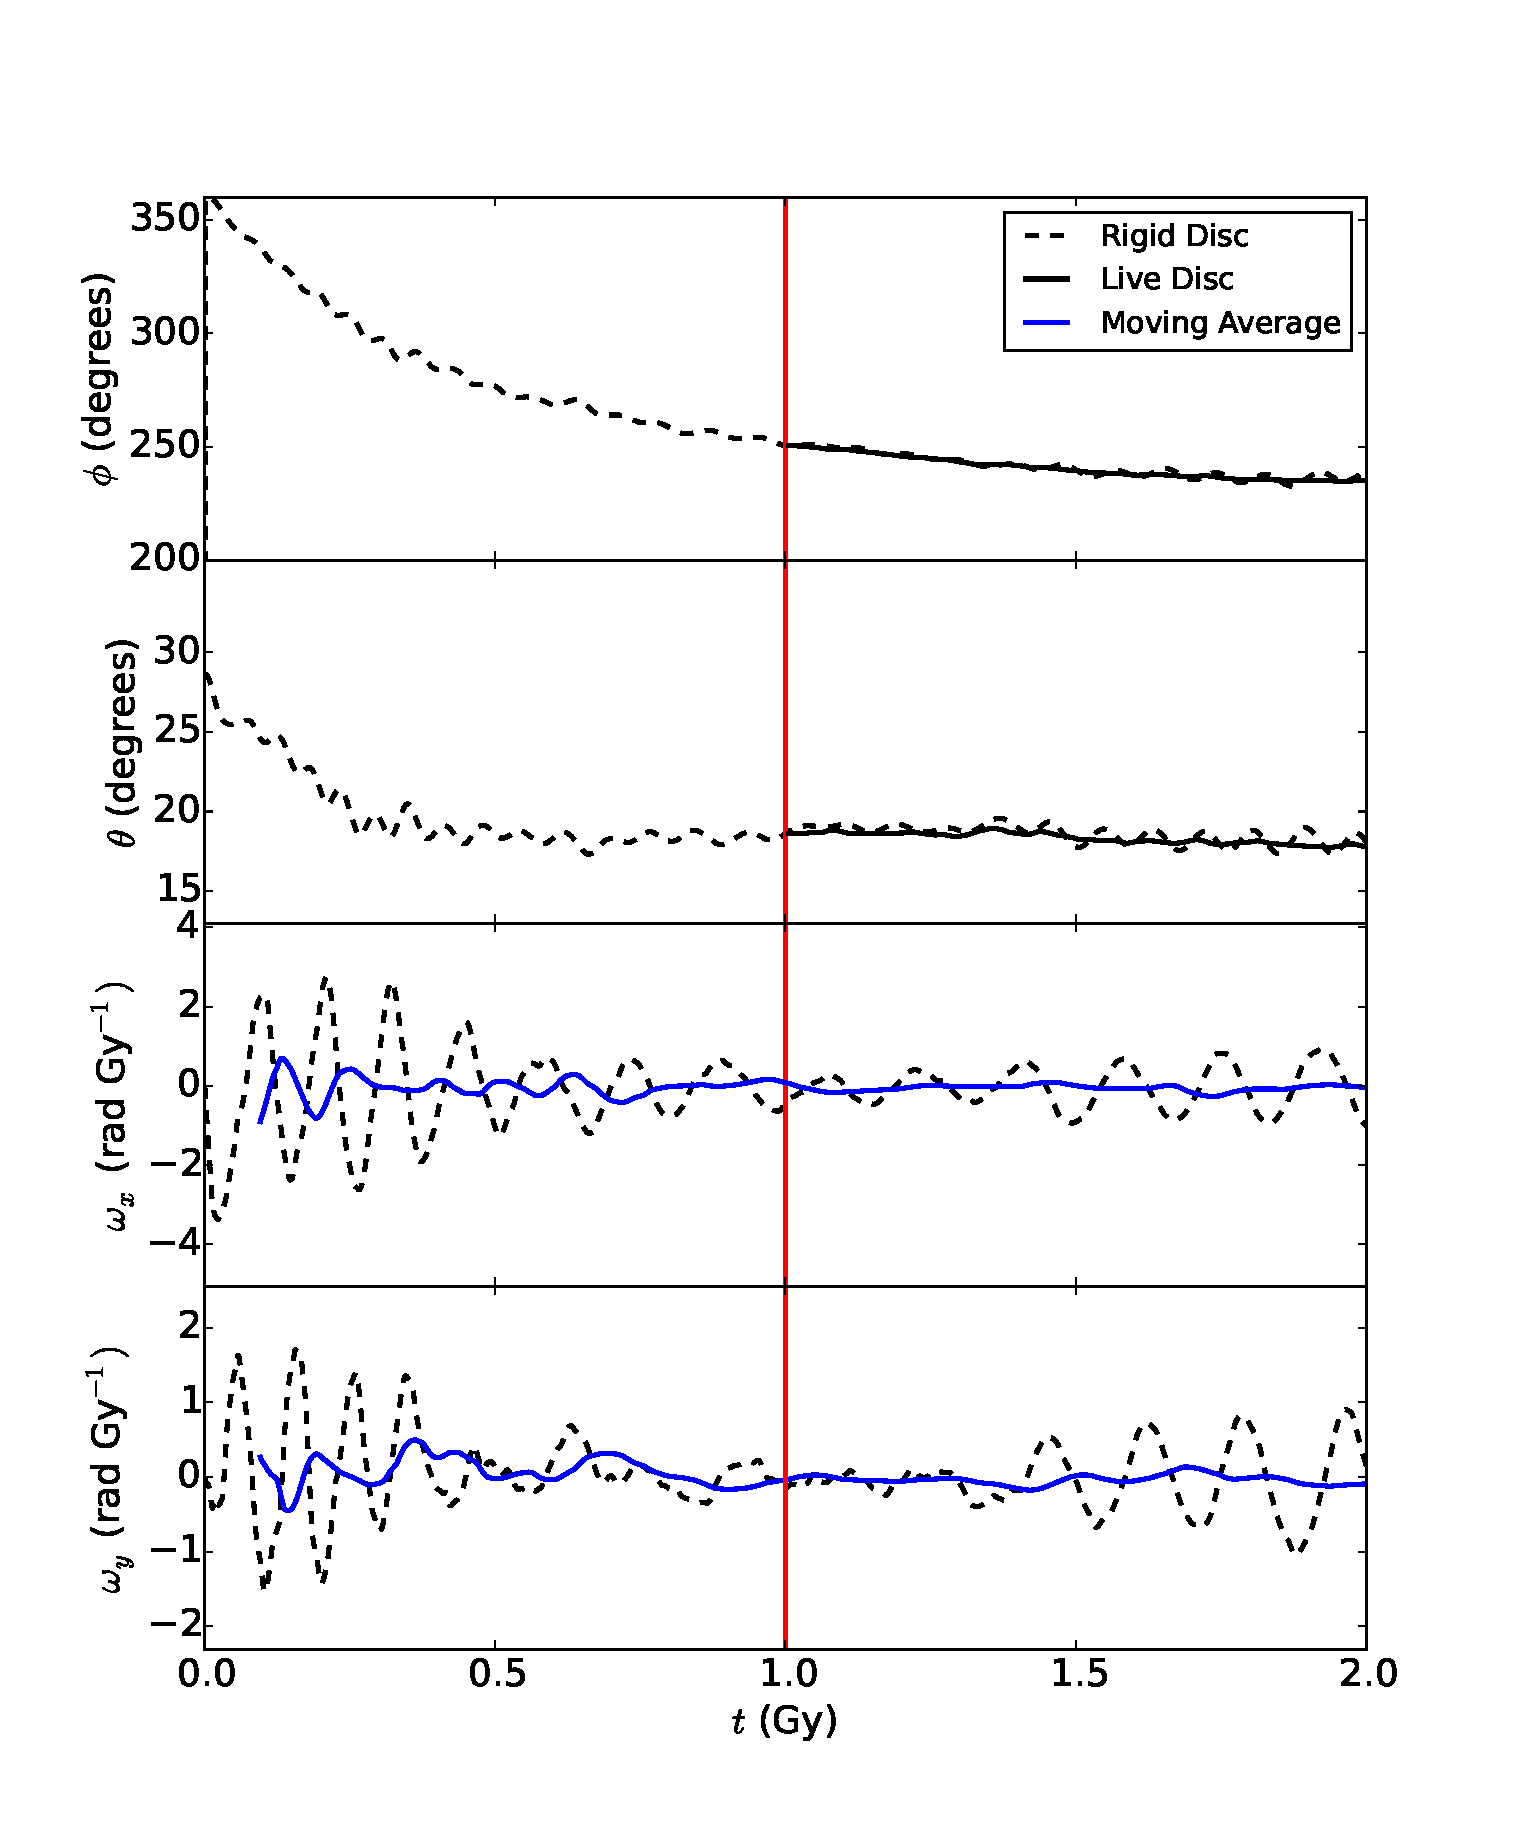
\includegraphics[width=0.9\textwidth]{../figures/flattened_halo_regressions.eps}
\caption{Kinematic variables for the rigid and live discs in an
  isolated, flattened halo as a function of time.  The upper two
  panels show the Euler angles $\theta$ and $\phi$ for the rigid disc
  (dashed curves) and live disc (solid curves) where the live disc is
  introduced at $t=1\,{\rm Gyr}$ (red vertical line).  The bottom two
  panels show the $x$ and $y$ components of the angular velocity, as
  measured in the body coordinate system.  In these two panels the
  solid curves show the $\delta t \sim 150\, \text{My}$ moving
  average, which is used to initialize the live disc.}
\label{fig:flattened_halo_regression}
\end{figure}
  
Fig. \ref{fig:flattened_halo_regression} shows the Euler angles and
angular velocity components for the rigid and live discs as a function
of time.  The time-dependence of $\omega_x$ and $\omega_y$ is
characterized by an interference pattern between short $\sim 125\,{\rm
  Myr}$ period nutations and a decaying long-period
precessional motion. Note that $\theta$ and $\phi$ for the live disc
track the corresponding values for the rigid disc for $t>1\,{\rm
  Gyr}$.  By initializing the live disc with the angular velocity of
the rigid disc, we capture the (small) precessional motion of $\sim
10^\circ {\rm Gyr}^{-1}$ between $t = 1\,{\rm Gyr}$ and $2\,{\rm
  Gyr}$.  The disc settles into a preferred plane within the first
$300\,{\rm Myr}$ that is intermediate between its initial symmetry
plane and the initial symmetry plane of the halo. More precisely, the
vector of the new minor axis is $\textbf{c} = [-0.159,0.146,0.976]$
measured at $20\text{ kpc}$, $12.5^{\circ}$ from the original
flattening axis.

\begin{figure}
\centering 
\includegraphics[width=0.9\textwidth]{../figures/Flattened_Selected_Density_Panels.eps}
\caption{Face-on projections of the particle distribution for two
  snapshots of a live disc in a flattened
  halo. The solid line for scale is 25 kpc with a centre
  coincident with the disc's. }\label{fig:flattened_disk_warps}
\end{figure}

\begin{figure}
\centering
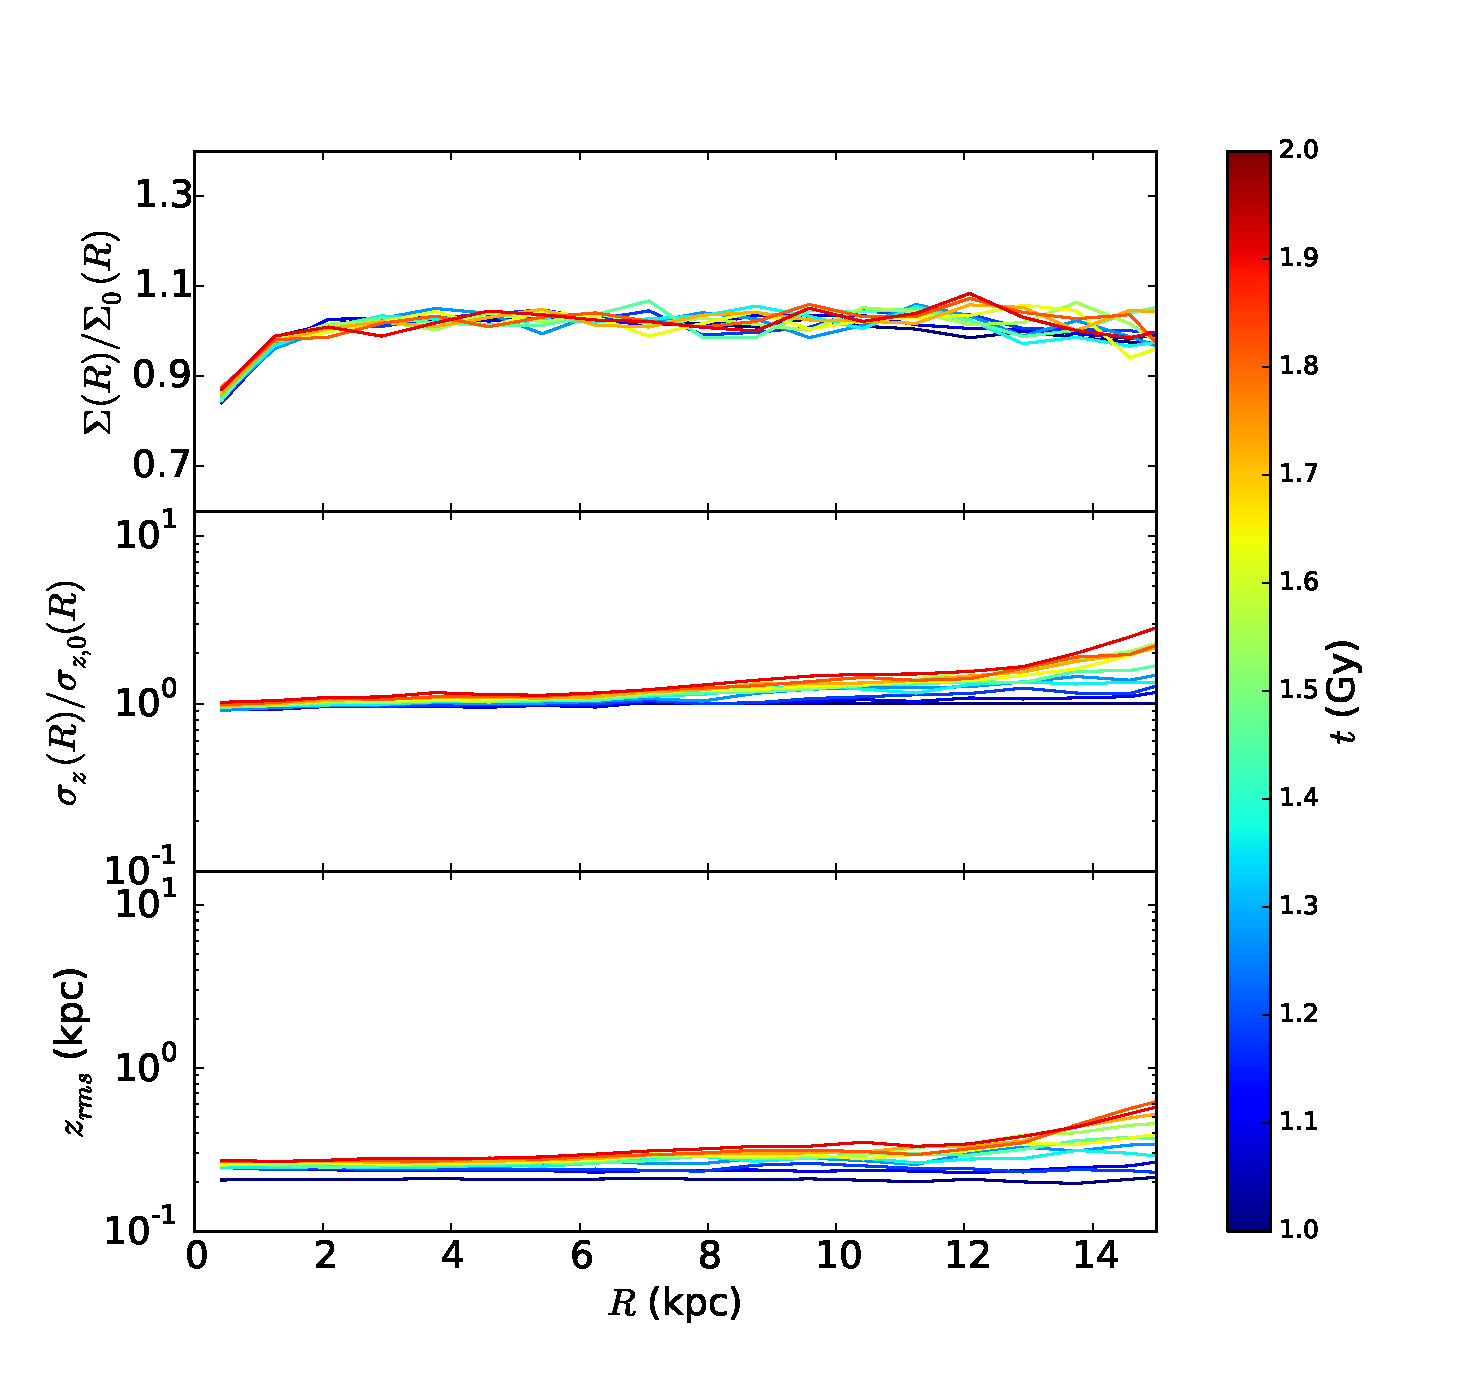
\includegraphics[width=0.9\textwidth]{../figures/flattened_surface_densities_fixed.eps}
\caption{Surface density, vertical velocity dispersion, and scale
  height profiles as a function of Galactocentric radius $R$ for 10
  snapshots equally spaced in time.  The top panel shows the surface
  density $\Sigma(R)$ divided by
  $\Sigma_0(R) = \left (M_d/2\pi R_d^2\right )\exp{\left[-\left
        (R/R_d\right ) \right]}$
  in order to highlight departures from a pure exponential disc.
  Likewise, in the middle panel, we show the ratio
  $\sigma_z(R)/\sigma_{z,0}(R)$ where $\sigma_{z,0} = \exp{(-R/2R_d)}$.
  The bottom panel shows the RMS $z$ as a function of $R$. }
\label{fig:flattened_surface_densities}
\end{figure}

Fig. \ref{fig:flattened_disk_warps} shows surface density maps for the
disc at two snapshots.  The disc develops a weak warp due to its
interaction with the halo.  The development of the warp is also
evident in the surface density, vertical velocity dispersion, and
scale height profiles shown in
Fig. \ref{fig:flattened_surface_densities}.  We see that the surface
density within $\sim 15\,{\rm kpc}$ or $6R_d$ is essentially unchanged
while at larger radii, there are $10-20\%$ time-dependent
fluctuations.  The scale height $\langle z^2\rangle^{1/2}$ increases
with time and radius.  At early times, the increase is most prominent
beyond $\sim 15\,{\rm kpc}$ while at late times, the scale height
increases more smoothly from the center to the edge of the disc.

\section{Cosmological Simulations}

We now use our method to insert a live disc with prescribed structural 
properties into a cosmological halo.  In this section, we focus on 
disc dynamics while in the next, we consider the effect the disc has 
on the dark halo. 

\begin{figure}
\centering
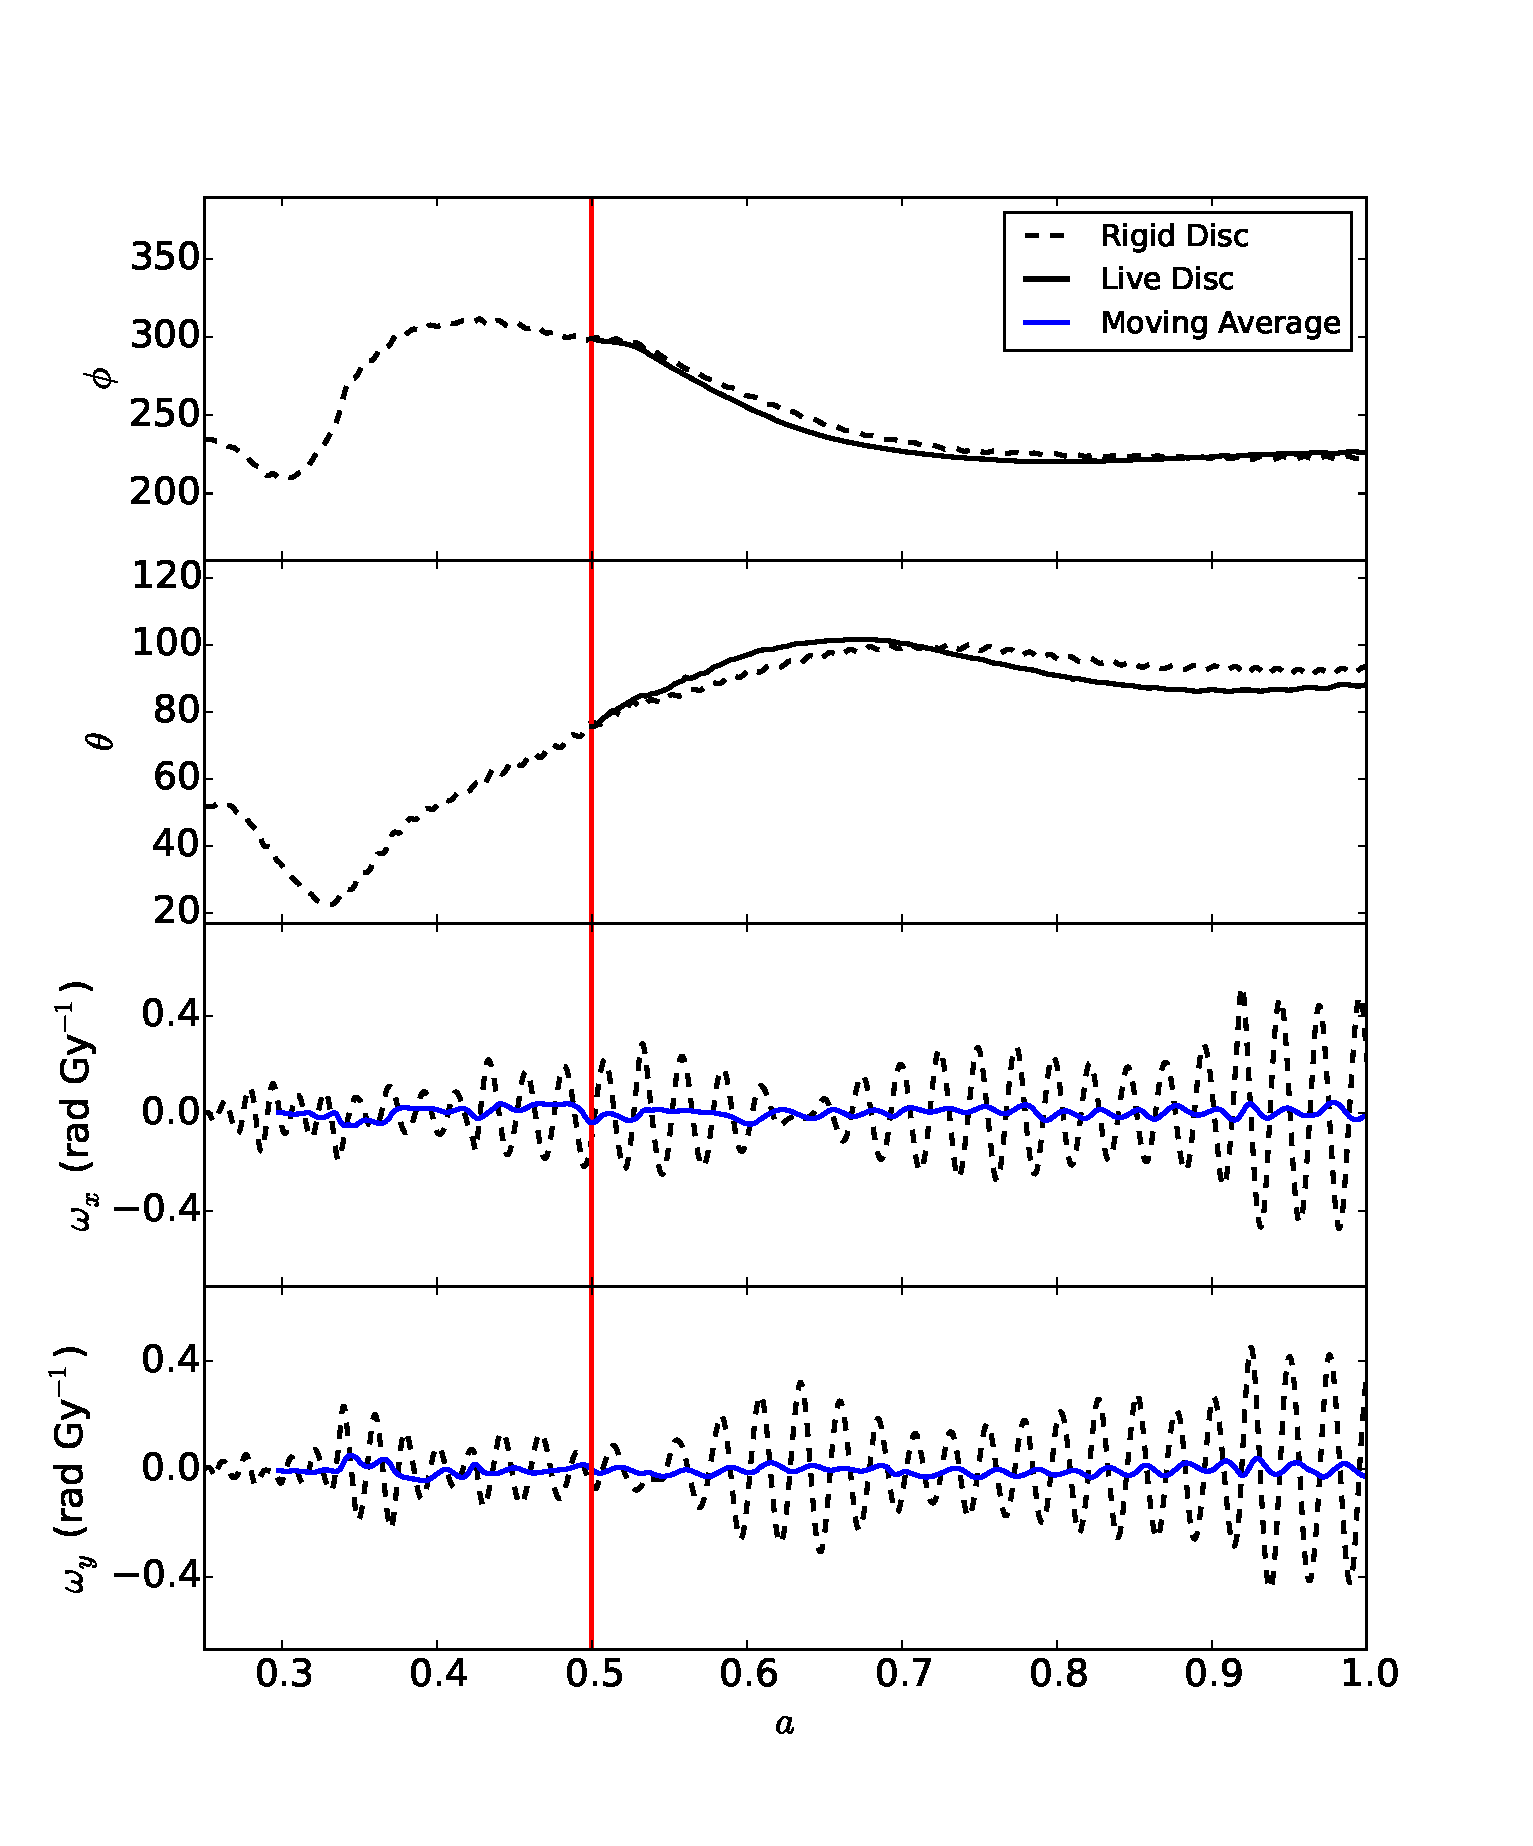
\includegraphics[width=0.9\textwidth]{../figures/cosmo_halo_regressions.eps}
\caption{Kinematic variables for the rigid and live discs in our
  cosmological halo as a function of scale factor $a$.  Line types are
  the same as in Fig. \ref{fig:flattened_halo_regression}.  The live
  disc is introduced at a redshift $z=1$ when the scale factor is
  $a=0.5$ (red vertical line). The blue line shows the $\delta a \sim
  0.04$ moving average calculated by averaging the last 300 points in
  the disc integration routine.} \label{fig:cosmo_inclination}
\end{figure}

In Fig.\,\ref{fig:cosmo_inclination} we show the kinematic variables
for the rigid and live discs in the RD and LD simulations.  The two
simulations are identical prior to $z=1$ ($a=0.5$) when the live disc
is swapped in for the rigid one.  The short period ($300\,{\rm Myr}$)
oscillations in $\omega_1$ and $\omega_2$ are nutations.  To
initialize the live disc, we use the fixed-window moving average of $\omega_x$ and
$\omega_y$.  By and large, the Euler angles of the rigid and live
disc's track one another for $z<1$, indicating that the rigid disc
is a reasonable model for a live one, at least in terms of the disc's
orientation.

\begin{figure}
\centering 
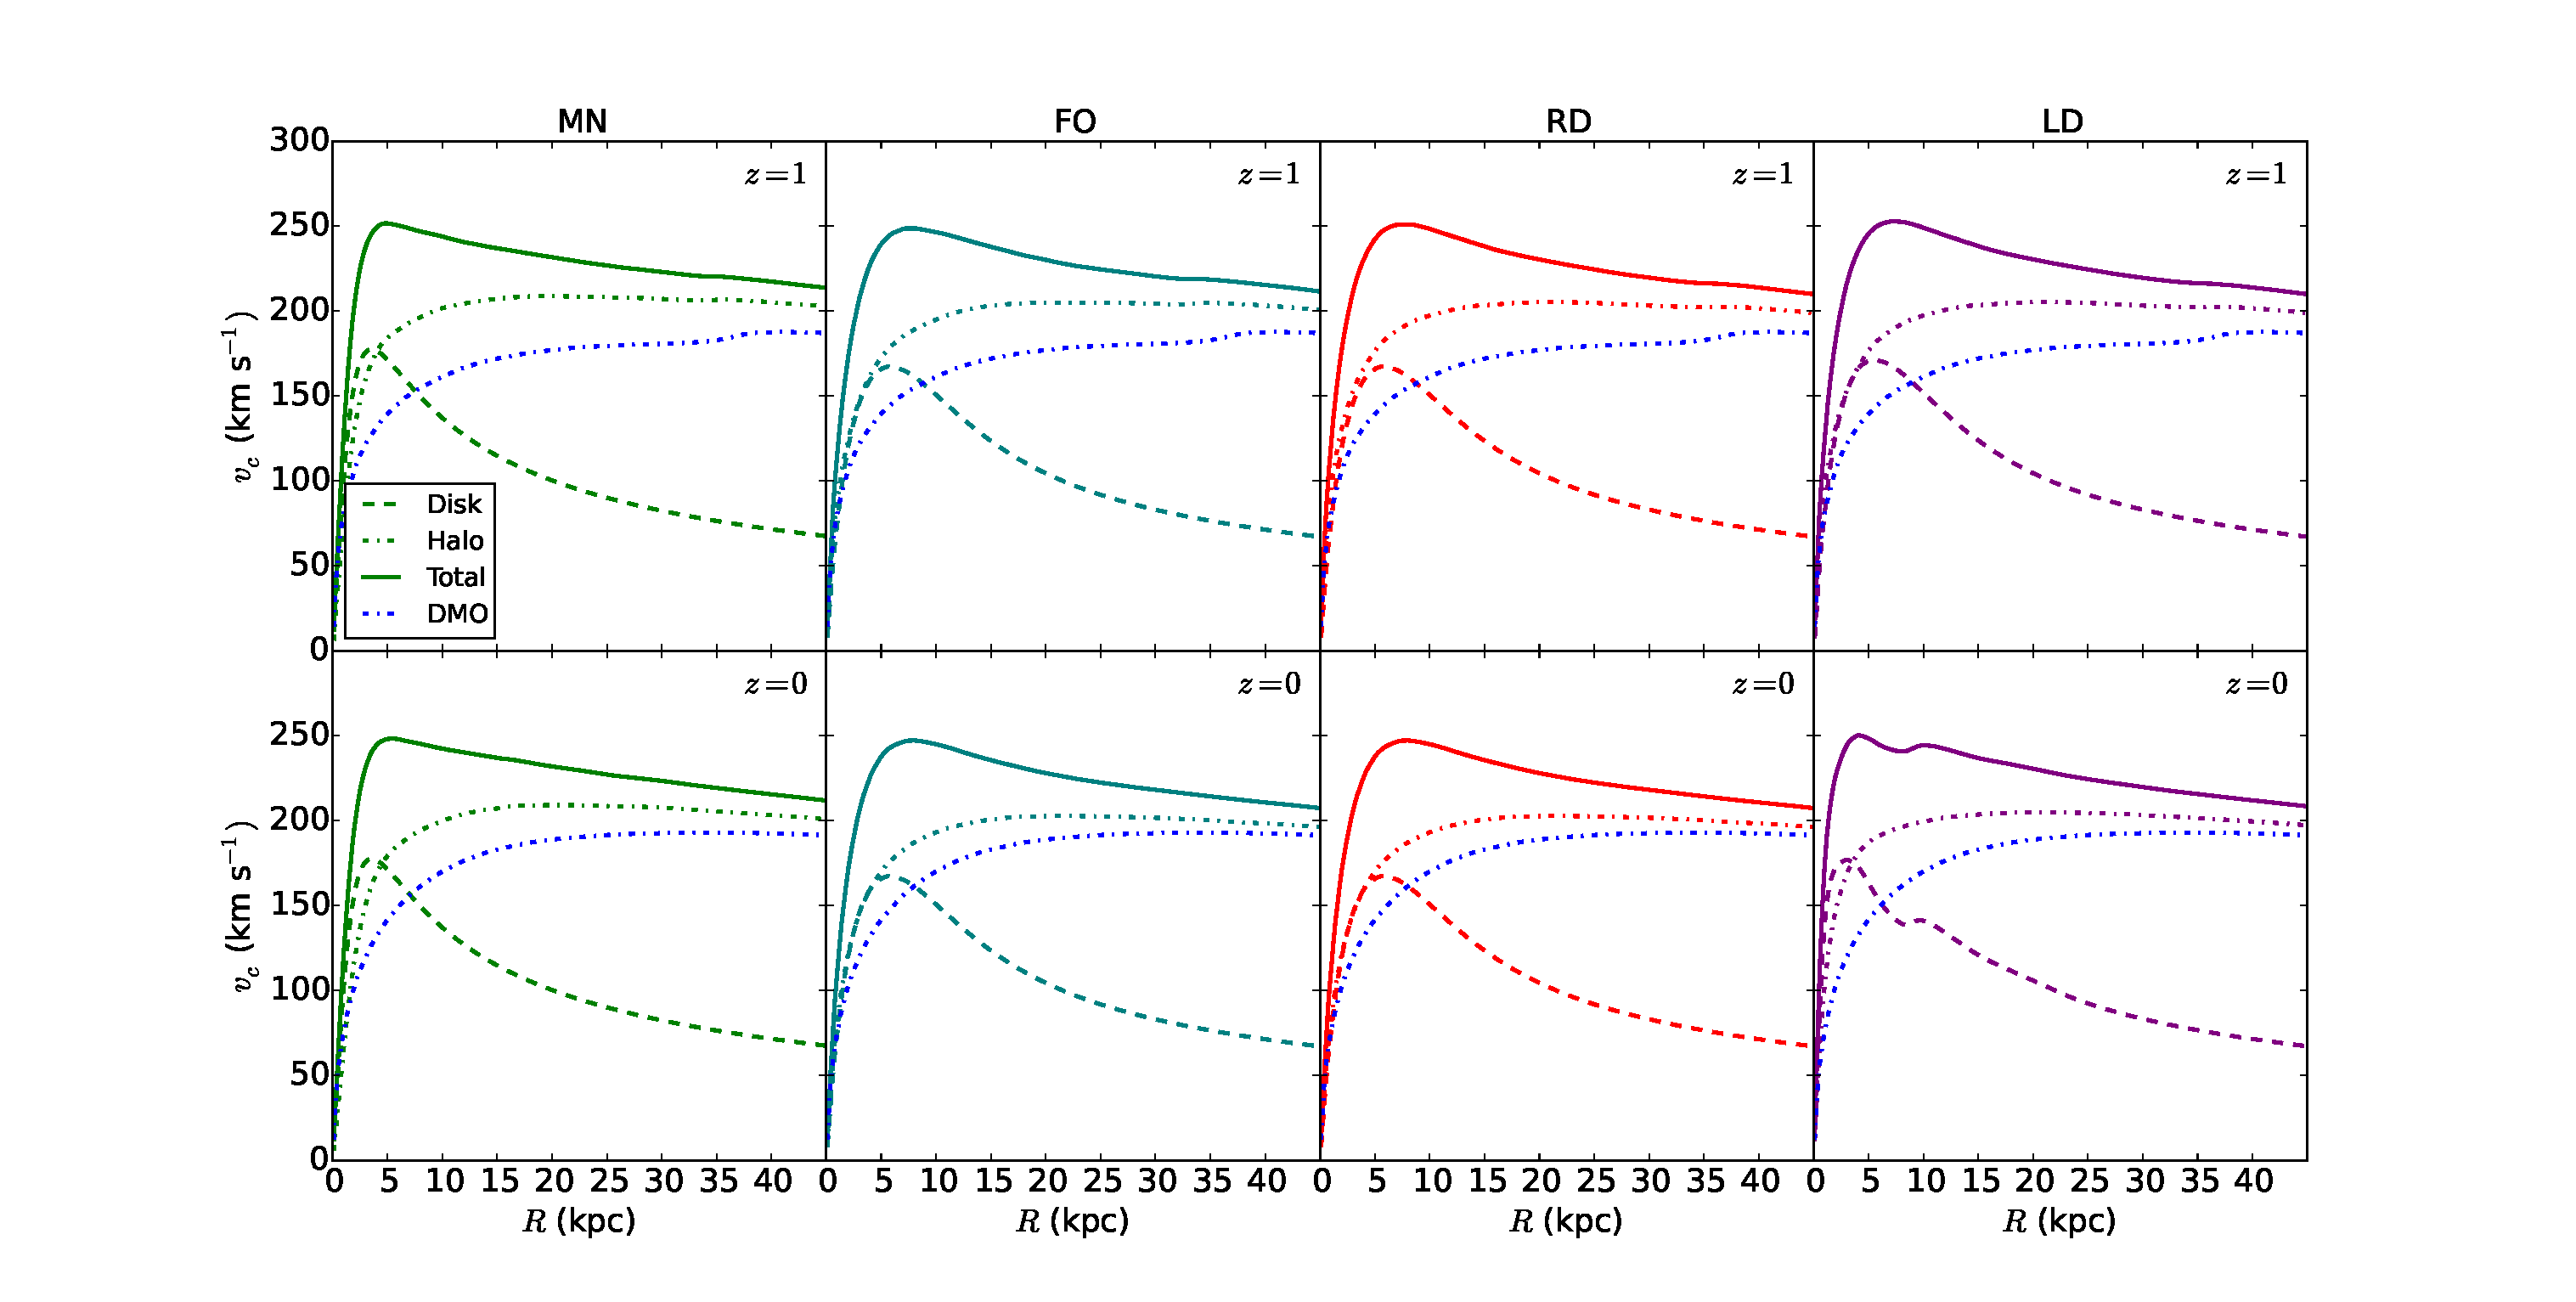
\includegraphics[width=1.\textwidth]{../figures/all_rotation_curves_five_sims}
\caption{Circular speed curve decompositions at $z=1$ (top row) and
  $z=0$ (bottom row) for (from left to right) our MN, FO, RD, and LD
  simulations.  Halo contributions are represented as dot-dashed
  lines, disc contributions are represented by dashed lines, and the
  total rotation curve is given by a solid line.  For reference, we have
  included the circular speed curve for the DMO halo (dot-dashed curve).}
\label{fig:rotation_curves}
\end{figure} 

In Fig.\,\ref{fig:rotation_curves} we show the circular speed curves
at $z=1$ and $z=0$ for our four simulations.  We see that the disc in
our model is submaximal.  To be precise, we have $V_d/V_c \simeq 0.68$
at $R=2.2R_d$ where $V_d$ is the circular speed due to the disc and
$V_c$ is the total circular speed.  In short, the contributions from
the disc and halo to the centrifugal force are approximately equal at
a radius where the disc contribution reaches its peak value.  By
comparison, a maximal disc is generally defined to have $V_d/V_c >
0.85$ \citep{sackett1997}.  If we use $V_d/V_c$ at $2.2R_d$ as the
defining characteristic of the model, then our simulations match up
with the F-5 simulation of
\citet{YurinSpringelStellarDisks}, although our discs are slightly
warmer, with a Toomre Q-parameter of $1.4$ as compared with $Q\simeq
0.9$ for their discs and our discs are thinner ($200\,{\rm pc}$ vs.
$600\,{\rm pc}$). We note that in a two-integral disc DF, $Q$ and the
disc thickness are linked whereas in a three-integral DF, they can be
set independently.  The method of \citet{YurinSpringelGalic} can be extended to consider
a three-integral DF, but these models were not considered in  \citet{YurinSpringelStellarDisks}. Moreover, their two-integral model, 
which imposes $\sigma_R=\sigma_z$, violates the epicycle approximation,
leading to transient system behaviour at early times when disc bars
first form.

%\textbf{Although the GalIC code can be extended to consider models for which $\sigma_R \neq \sigma_z$, these models will not be in equilibrium as GalIC does not enforce consistency with the epicycle approximation \citep{AumerBinneyGalICComments}}.
%In other words, the models considered in
%\citet{YurinSpringelStellarDisks} are a restricted subset of possible
%disc models.

The circular speed curves in Fig. \ref{fig:rotation_curves} show little change exterior to $\sim 2R_d$
after $z_l$, thus providing another indication that the live disc
was close equilibrium when it was swapped in for the rigid one. The
formation of a bar is evident in the circular speed, and we can infer
the bar contributes substantially inside $2.2 R_d \simeq 8$\,kpc.  The halo contribution at $R=2.2R_d$ is about 20\% larger
in the four disc runs than in the DMO one due to adiabatic
contraction.  Interestingly, the halo in the MN run shows
somewhat more contraction than in the RD and LD runs.  We note that in
the MN run, the disc potential tracks the potential minimum of the
halo whereas in the RD/LD case, the disc's position is determined from
Newtonian dynamics.  In general, the centre of the disc tracks the
halo potential minimum so long as the potential changes slowly with
time.  However, during a major merger (and indeed, just such an event
occurs at $z=2$) there are rapid changes in the halo potential and 
the position of the disc, as determined by Newtonian dynamics, can
differ significant from the minimum of the halo potential.  Evidently,
the {\it ad hoc} prescription of growing a disc at the halo's
potential minimum may, in some cases, over-estimate the effect of
adiabatic contraction.

\begin{figure}
\centering
\includegraphics[width=0.9\textwidth]{../figures/Selected_Density_Panels.eps}
\caption{Projected density along three orthogonal directions for the
  live disc at four epochs between $z=1$ and $z=0$.  The projections are presented
  in physical units. The solid line for scale is
  37 kpc with a centre coincident with the disc's.}
\label{fig:cosmo_density_panels}
\end{figure}

\subsection{Bar Formation}

In Fig.\,\ref{fig:cosmo_density_panels} we show orthogonal projections
of the disc density in our LD simulation at four epochs between
$z=1$ (lookback time of 7.9 Gyr) and the present epoch.
During the first billion years of live disc evolution, the disc
develops a bar and spiral structure.  In addition, there is a
warp in the outer disc extending several kiloparsecs above the midplane
of the inner disc.  By the present epoch, the bar has grown in length and
intensified and the edge-on view shows the classic X-pattern.

We consider the usual parameter bar strength $A_2 = 
|c_2|$ where

\begin{equation}
c_m = \frac{1}{M_S}\sum_{j\in S} m_j e^{im\phi_j}~.
\end{equation}

\noindent Here, $S$ is some circularly-symmetric region of the disc
(e.g., a circular annulus) and the sum is over all particles labeled
by $j$ and with mass $m_j$ that are inside $S$.  We find that
$A_2$ for the inner $2R_d$ of the disc reaches $0.43$ at $t=6.7\,{\rm
  Gyr}$, decreases to $0.36$ by $t= 9.2\,{\rm Gyr}$, presumably
because the bar has buckled, and then increases to $0.47$ by the
present epoch.  On the other hand, $A_2$ for the entire disc increases
to $0.27$, decreases to $0.23$, and then increases to $0.28$ for the
same epochs.  Note that the inner $2R_d$ of the disc contains $60\%$
of the mass.  Thus, the fact that $A_{2,2R_d}/A_{2,{\rm tot}}\simeq
  0.6$ implies that most of the bar mass resides within the inner
  $2R_d$.

The bars in \citet{YurinSpringelStellarDisks} seem to be stronger then
then ones in our simulations --- they find $A_2\simeq 0.6$ but use a
non-standard formula for $A_2$.  Moreover, their bars appear to extend
across most of the disc.  In terms of disc dynamics, the main
difference between our simulations is the fact that we use a
three-integral DF for the disc whereas they use a two-integral DF.  In
the latter, the velocity dispersion in the radial and vertical
directions are the same.  Thus, the radial dispersion, which fixes the
Toomre $Q$ parameter, also determines the thickness of the disc.  We
note that their initial discs are a factor of two or three thicker
than ours.  We speculate that the bars that develop in these thick
discs are less susceptible to buckling and therefore able to grow
stronger and longer.  These ideas will be investigated in more detail
in a future publication.

\subsection{Kicked-up Stars and Disc Heating}

The outer part of the disc suffers considerable disruption and warping
presumably through its interaction with the main halo or substructure.  The right-most
panel of the $a=0.55$ snapshot in Fig. \ref{fig:cosmo_density_panels}, for example, shows a classic
integral-sign warp.  The other snapshots show that a significant
number of disc particles have orbits that now take them to high
galactic latitudes.

\begin{figure}\centering 
 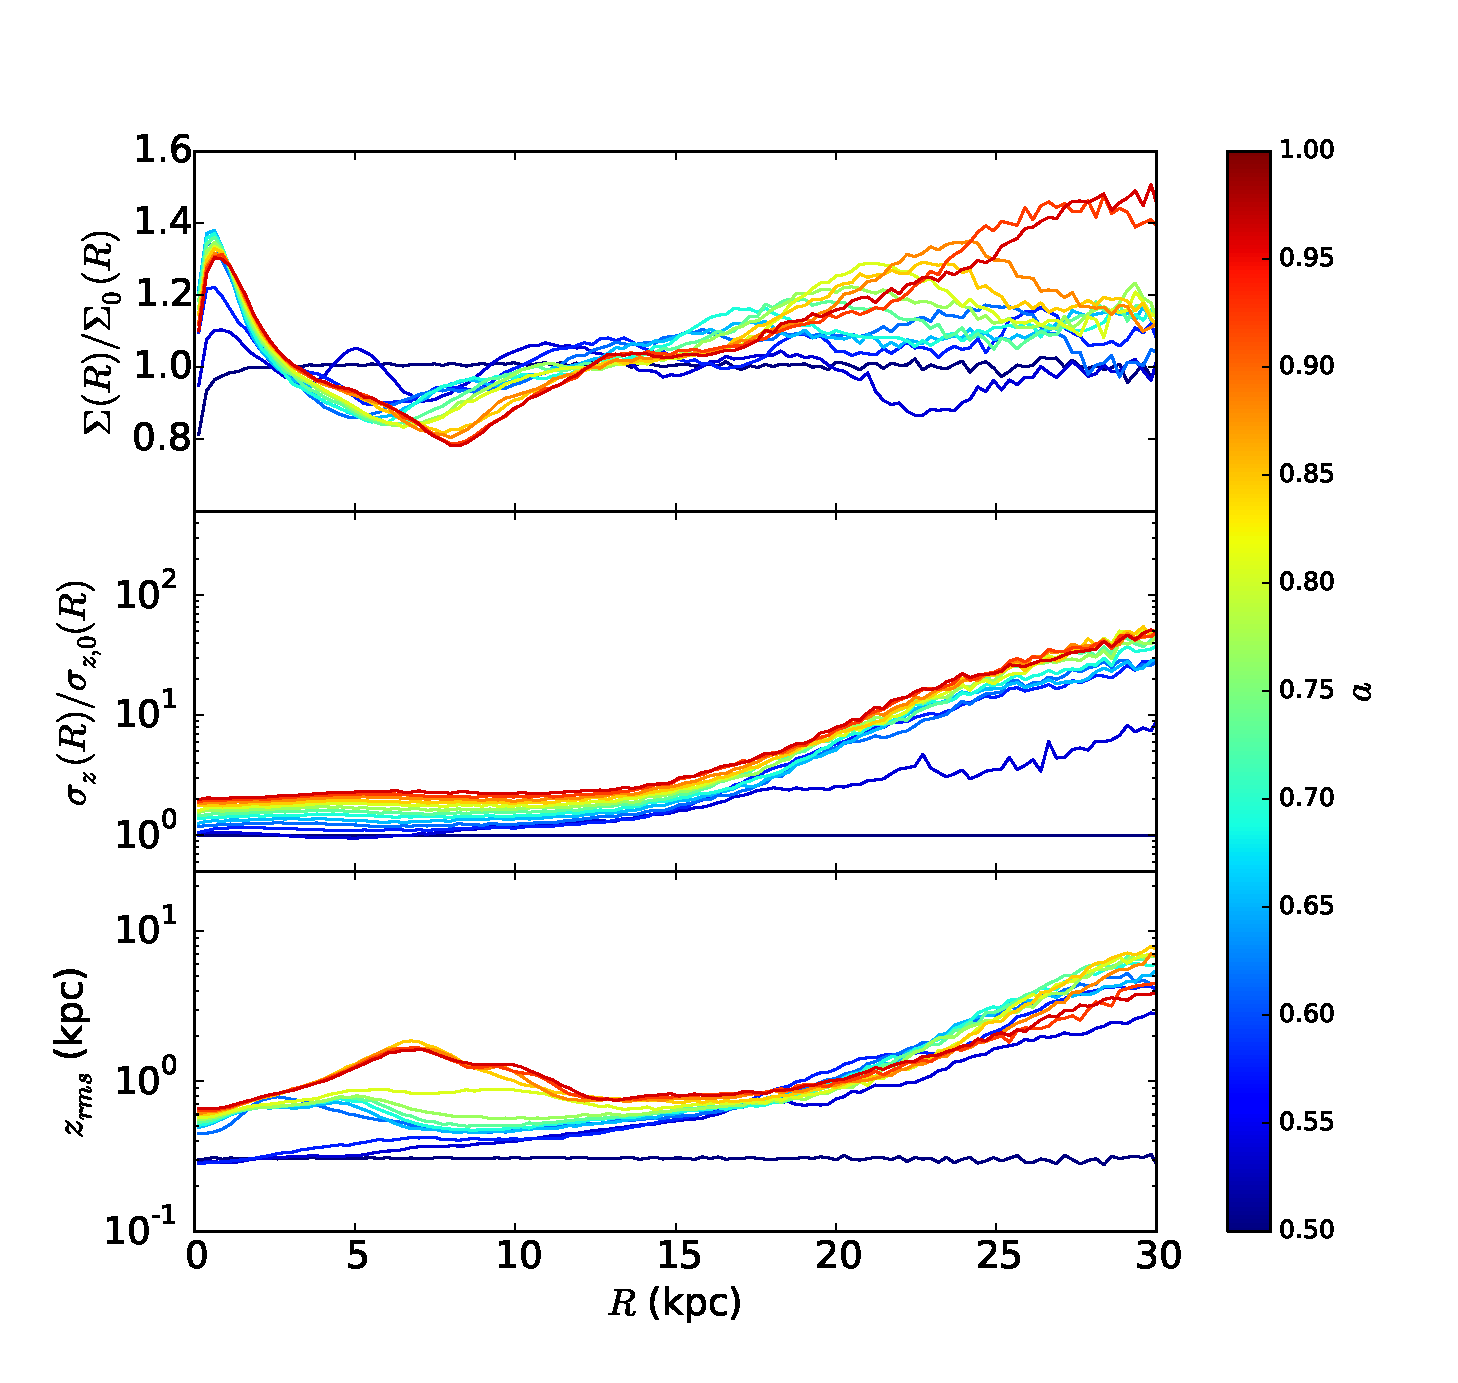
\includegraphics[width=0.9\textwidth]{../figures/surface_densities.eps}

  \caption{Surface density, vertical velocity dispersion, and scale
    height profiles of the live disc for 10 snapshots equally spaced
    in scale factor $a$ between $a=0.5$ ($z=1$) and $a=1$ (present
    epoch).  Panels are the same as in
    Fig. \ref{fig:flattened_surface_densities}.}
\label{fig:surface_densities} 
\end{figure}

The impressions one has from the density projections are borne out in
Fig.\,\ref{fig:surface_densities} where we show the surface density
and scale height profiles at different times.  Bar formation
redistributes mass in the disc leaving a deficit (relative to the
initial exponential disk) between $5$ and $15\,{\rm kpc}$.  The disc
becomes thicker and its vertical velocity dispersion increases though
a combination of disc-halo interactions and the effects of the bar and
spiral structure \citep{gauthier2006, dubinski2008, kazantzidis2008}.

A striking feature of the simulations are the streams of disc stars
well above the disc plane.  These stars may represent an example of a
kicked-up disc, which has been seen in other N-body simulations
\citep{PurcellHeatedDisk, McCarthyHeatedDisk} and invoked to explain
kinematic and spectroscopic observations of M31
\citep{DormanKickedUpDisk} and the Monoceros Ring \citep[e.g.][]{monoceros_disc,ibata_et_al_2003}. The idea is that interactions between the
disc and both satellite galaxies and halo substructure liberate stars
from the disc, launching them to regions of the galaxy normally
associated with the stellar halo.  Our live disc simulation
corroborates this hypothesis and is in broad agreement with previous
numerical work. 

Finally, we note that the $a=1$ panel of Fig. \ref{fig:cosmo_density_panels}
shows a relatively thin, stream-like structure, above the disc which
is qualitatively similar to the Anti-centre Stream \citep[ACS,][]{acs_disc}. While the ACS
is believed to be due to the disruption of a globular cluster \citep[e.g.][]{acs_disc}, Fig. \ref{fig:cosmo_density_panels} suggests that perturbations to the disc can create similar features. Intriguingly, \citep{de_boer_et_al_2017} recently 
found that the ACS is rotating in the same sense as the Milky Way disc.


%{\bf There is also some basis for believing that there are similarly 
%kicked up disc stars in the Milky Way.  The Monoceros Ring is a Milky Way 
%structure composed of low-metallicity stars in a narrow range of Galactocentric
%distances (15-20 kpc) \citep{newberg2002, yanny2003, monoceros2005}. Two 
%competing hypotheses for the formation of the Monoceros stream of stars are
%a dwarf galaxy on a near circular orbit at low Galactic latitude, or displaced
%disc stars. Recent simulation and observational work suggests that the latter of
%these hypotheses could be at work in the Milky Way \citep{NewbergRadialWaves, gomezwarps}.
%Because our method allows us to study the evolution of an initially cold population of
%disc stars, we can resolve structures like the Monoceros Ring.  The fact that we find
%a similar structure in the one simulation we ran suggests, with existing work, that 
%perturbations to the disc's vertical structure may be a commonplace mechanism for 
%generating streams of stars coincident with the discs of galaxies.}

\section{Halo Substructure in the Presence of a Disc}

In this section, we consider the effect of a disc on a halo's
structural properties such as its spherically-averaged density
profile, its shape, and its subhalo population.  An examination of the
DMO simulation shows that the halo we have selected builds up through a
series of mergers and accretion events, but that by $z=1$ it has
settled into a relatively relaxed state with an NFW profile that
evolves very little between $z=1$ and $z=0$ within the inner 100 kpc.  Our sequence of
simulations, (MN, FO, RD, and LD) allow us to tease out the effects of
different disc insertion methods.  The MN simulation, for example,
pins the centre of the disc to the minimum of the halo potential,
whereas the other simulations dynamically evolve the position and
velocity of the disc potential via Newtonian mechanics.  The MN and FO
simulations both assume that the orientation of the disc potential
during the growth phase is fixed whereas RD and LD solve for the
orientation using rigid body dynamics.
 
\subsection{Global Properties of the Halo}

\begin{figure} \centering 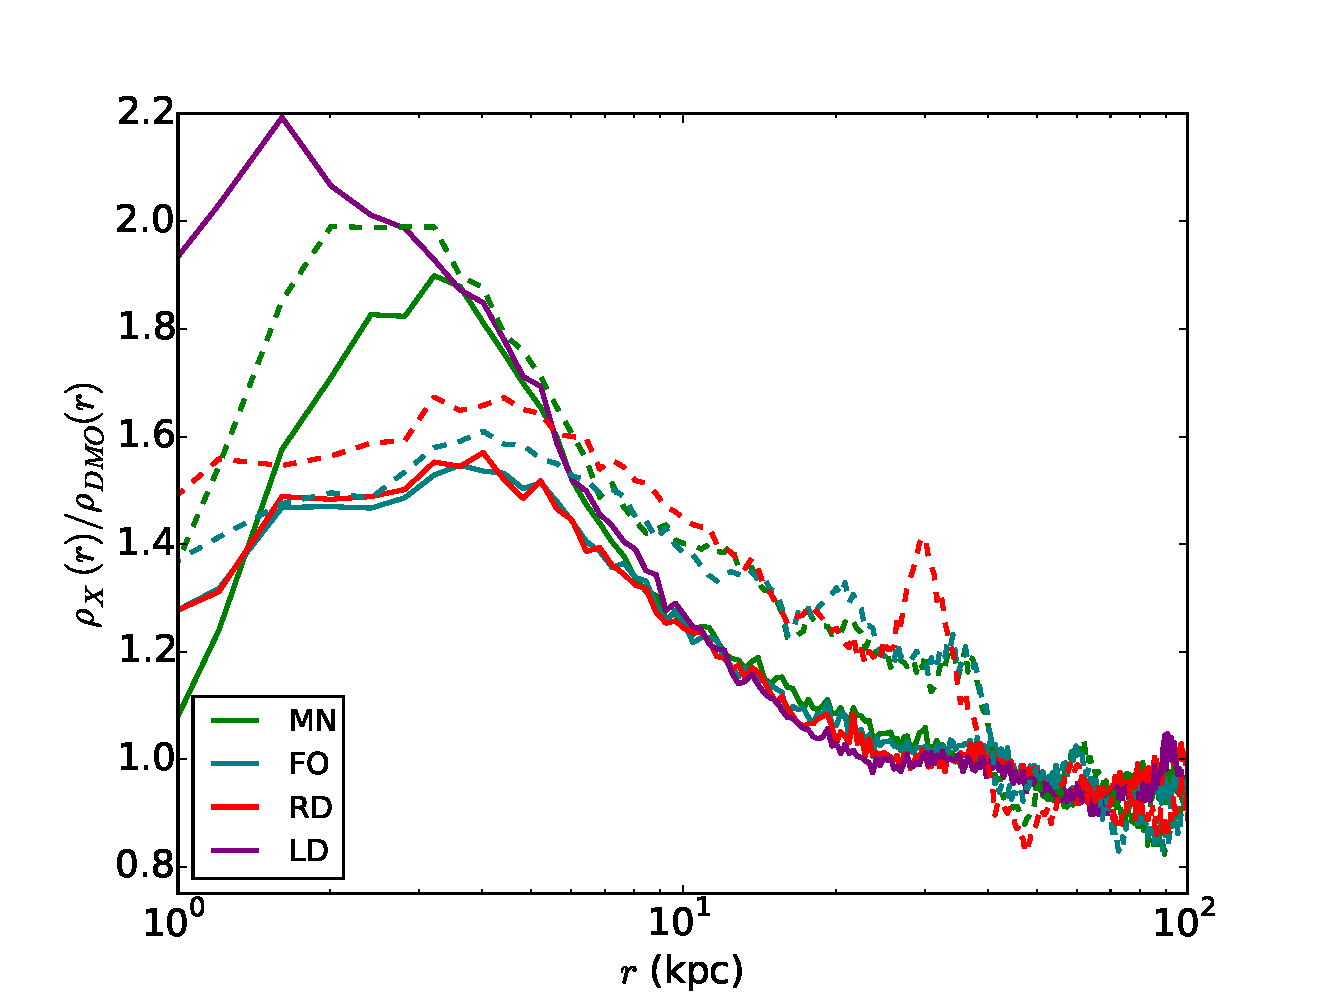
\includegraphics[width=0.9\textwidth]{../figures/halo_density_ratios_five_sims.eps} 
  \caption{The ratio of halo density to the DMO simulation for MN
    (green), FO (teal), RD (red), and LD (purple) at $z=1$ (dashed)
    and $z=0$ (solid). The presence of the disc significantly increases the central concentration of the halo.}
\label{fig:halo_ratios}
\end{figure}

In Fig.\,\ref{fig:halo_ratios} we show the ratio of the
spherically-averaged density profile in the four disc runs to that
from the DMO run.  At $z=1$ the haloes in the FO, RD, and MN runs show
evidence for adiabatic contraction with the density in the inner $\sim
30\,{\rm kpc}$ increasing by a factor of $1.2-2.1$.  The effect is
strongest in the MN simulation, which is to be expected since the halo
in that case always sees the disc potential at the minimum of its
potential.  Of course, this prescription is unphysical.  In general,
and especially during a major merger, the disc and halo potential
minimum will not necessarily coincide.

Between $z=1$ and $z=0$, the mass of the disc is constant.  Adiabatic
contraction ceases but the halo still responds to the time-varying
disc potential.  Interestingly, at intermediate radii (between
$\sim 10-40\,{\rm kpc}$) the density profile of the halo settles back
to a state close to that found in the DMO run.  Perhaps most striking
is the fact that the halo in the LD run becomes more centrally
concentrated than the halo in any of the other cases.  One possible explanation
is that dynamical friction from the disc drags dark matter subhaloes
toward the centre of the halo where they are tidally disrupted.

\begin{figure} 
\centering 
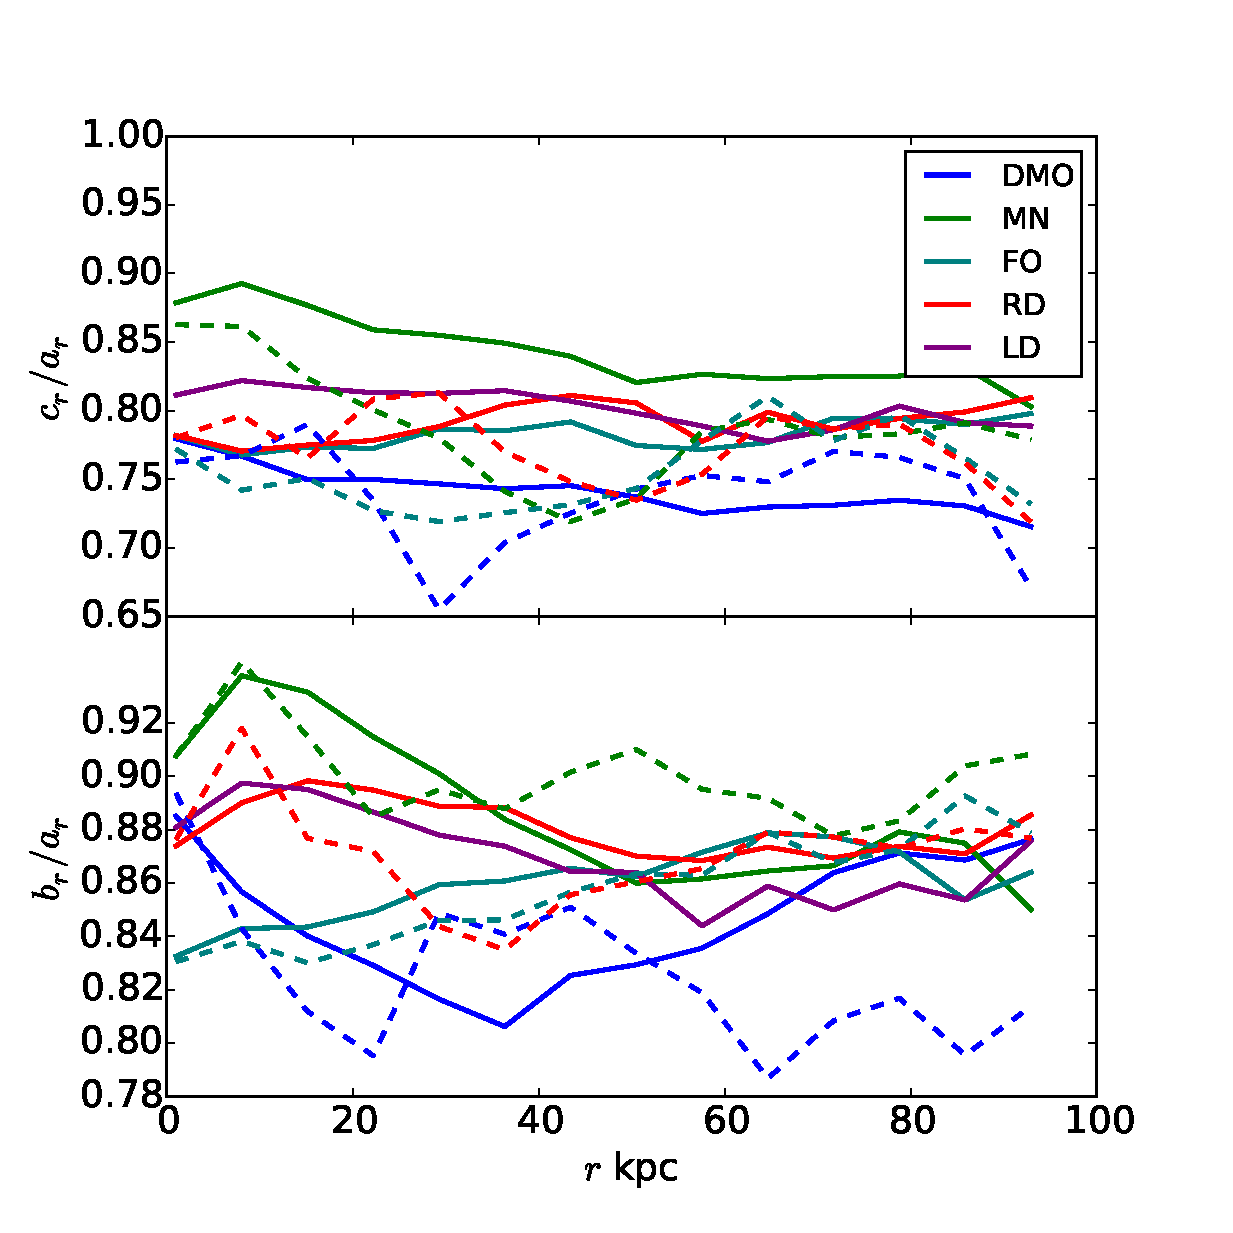
\includegraphics[width=0.9\textwidth]{../figures/eigenratios_vs_radius.eps} 
\caption{Axis ratios as a function of radius.  Shown are the
  minor-to-major axis ratio (top panel) and the intermediate-to-major
  axis ratio (bottom panel) at $z=1$ (dashed curves) and $z=0$ (solid
  curves).  Blue corresponds to DMO, green to MN, teal to FO, red to RD, and
  purple to LD.}
\label{fig:axis_ratios}
\end{figure}

In Fig.\,\ref{fig:axis_ratios} we show the minor-to-major ($c_r/a_r$)
and intermediate-to-major ($b_r/a_r$) axis ratios as a function of
radius for both the $z=1$ and $z=0$ snapshots.  The axis ratios are
calculated by diagonalizing the moment of inertia tensor in
linearly-spaced radial shells.  The DMO halo is triaxial with
$c_r/a_r\simeq 0.75$ and $b_r/a_r\simeq 0.85$.  Note that the axis
ratio profiles are smoother at $z=0$ than at $z=1$, which supports the
observation that the halo has settled into a more relaxed state over
the past $7$ or so billion years.  In general, discs tend to make
halos more spherical, a result that has been known for some time from
both collisionless and hydrodynamical simulations
\citep[e.g.][]{dubinski1994_ApJ431_617,Zemp2012}.


Evidently, the MN halo is rounder, especially in the inner part, than
the FO halo.  Recall that the main difference between these two cases
is that the MN disc is pinned to the potential minimum of the halo.
It is perhaps not surprising then that, as with adiabatic contraction,
it has a stronger effect on the halo's shape.  
We also note that the axis ratio profiles for the RD and LD simulations
are fairly similar.  

\subsection{Subhalo Populations}

We now turn our attention to halo substructure.  We identify subhaloes
and determine their positions and masses using \textsc{rockstar}
\citep{rockstar}, which employs a friends-of-friends algorithm in six
phase space dimensions.  We consider only those subhaloes with mass
$m_s$ between $m_{\rm min} = 10^{7.5}\,M_\odot$ and $m_{\rm max} =
10^{10.5}\,M_\odot$.  Subhaloes at the lower end of this range are
marginally resolved with $\sim100$ particles, above which the subhalo
mass can be trusted \citep[e.g.][]{onions_et_al_2012}, while those at the upper end contain $\sim 3\%$ of
the halo's virial mass.

\begin{figure} 
\centering 
{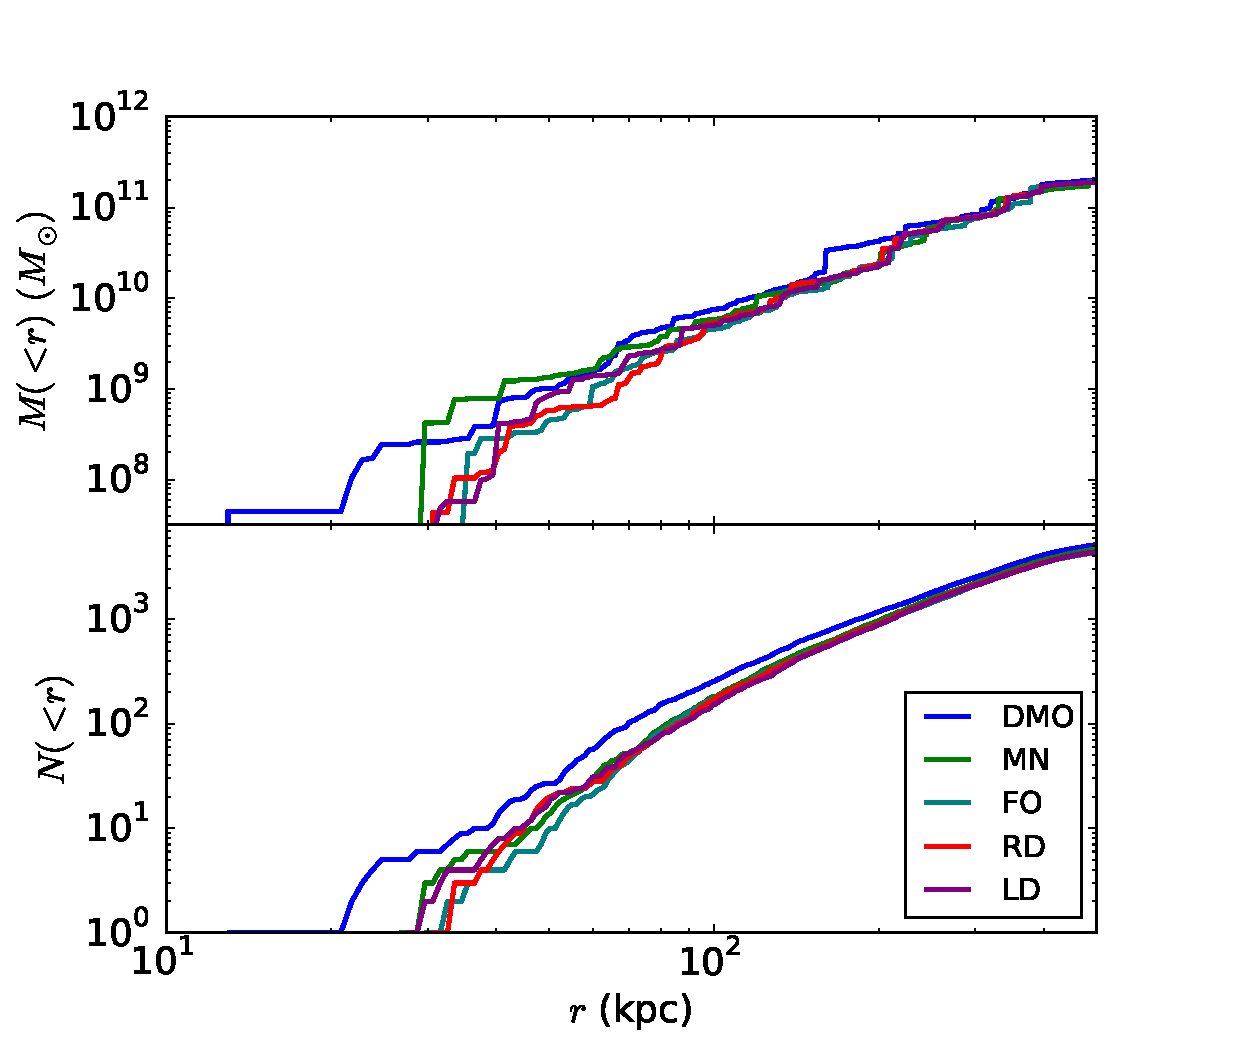
\includegraphics[width=0.9\textwidth]{../figures/cumulative_radial_distribution_five_sims.eps}}
\caption{Cumulative mass in subhaloes inside a radius $r$ (upper panel)
  and cumulative number of subhaloes (lower panel).  We consider only
  subhaloes within $500\,{\rm kpc}$ of the halo centre and with a mass
  above $10^{7.5} M_\odot$.  The curves are blue (DMO), green (MN),
  teal (FO), red (RD), and purple (LD).}
\label{fig:cumulative_distributions}
\end{figure}

\begin{figure} 
\centering 
{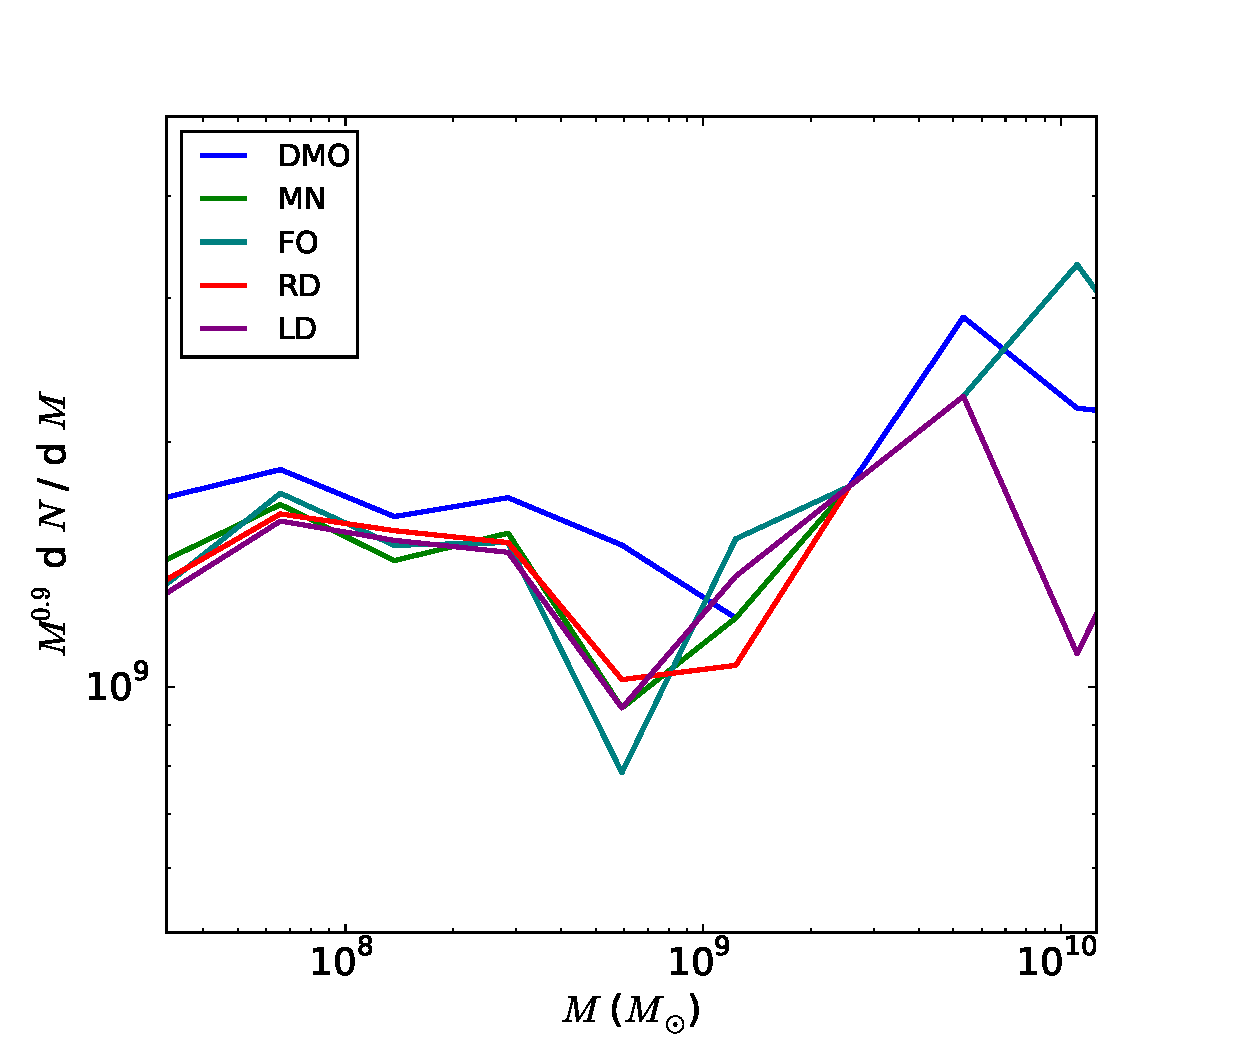
\includegraphics[width=0.9\textwidth]{../figures/differential_halo_mass_fn_five_sims.eps}}
\caption{ Differential mass distribution
  multiplied by $M^{0.9}$ for subhaloes above $10^{7.5} M_\odot$. We
  make an outer radius cut at 500 kpc. The curves are blue
  (DMO), green (MN), teal (FO), red (RD), and purple (LD). }
\label{fig:differential_mass_distributions}
\end{figure}

In Fig.\,\ref{fig:cumulative_distributions} we show the cumulative
mass in subhaloes as a function of Galactocentric radius:

\begin{equation}
M_s\left (<r\right )  = \int_0^r dr \int_{m_{\rm min}}^{m_{\rm
    max}} dm_s\,m_s\,\frac{d^2 N}{dm_s\,dr}
\end{equation}

\noindent We also show the cumulative number of subhaloes.  In
general, the presence of a disc depletes substructure inside about
$30\,{\rm kpc}$ but leaves the outer substructures unaffected.

We next consider the differential mass distribution as a function of
subhalo mass.  Recall that for a pure dark matter halo,
$dN/d\ln(m_s)\propto m_s^{-p}$ where $p\simeq 0.9$
\citep[e.g.][]{gao2004}.  In
Fig. \ref{fig:differential_mass_distributions}, we therefore show the
quantity $m^{0.9}\,dN/d\ln(m_s)$ in order to enhance the differences
between the different disc runs.  We see that the halo population
between $m_s \simeq m_{\rm min}$ and $m_s\simeq 10^9\,M_\odot$ is
depleted, but only by about $20-30\,\%$.  Taken together,
Fig.\,\ref{fig:cumulative_distributions} and
Fig. \ref{fig:differential_mass_distributions} imply that the main
depletion of the subhaloes occurs within the inner regions of the
parent halo, in agreement with \citet{DOhngiaSubstructureDepletion,Sawala2017,GKSubhaloDepletion17}.  That said, the depletion of subhaloes seems rather
insensitive to the disc insertion method, although we caution that only a single halo was used. Our results, being mainly in agreement with previous work, should still be viewed with caution due the consideration of a single host halo.

\subsection{Case Study: A Sagittarius-like Dwarf}

\begin{figure} \centering
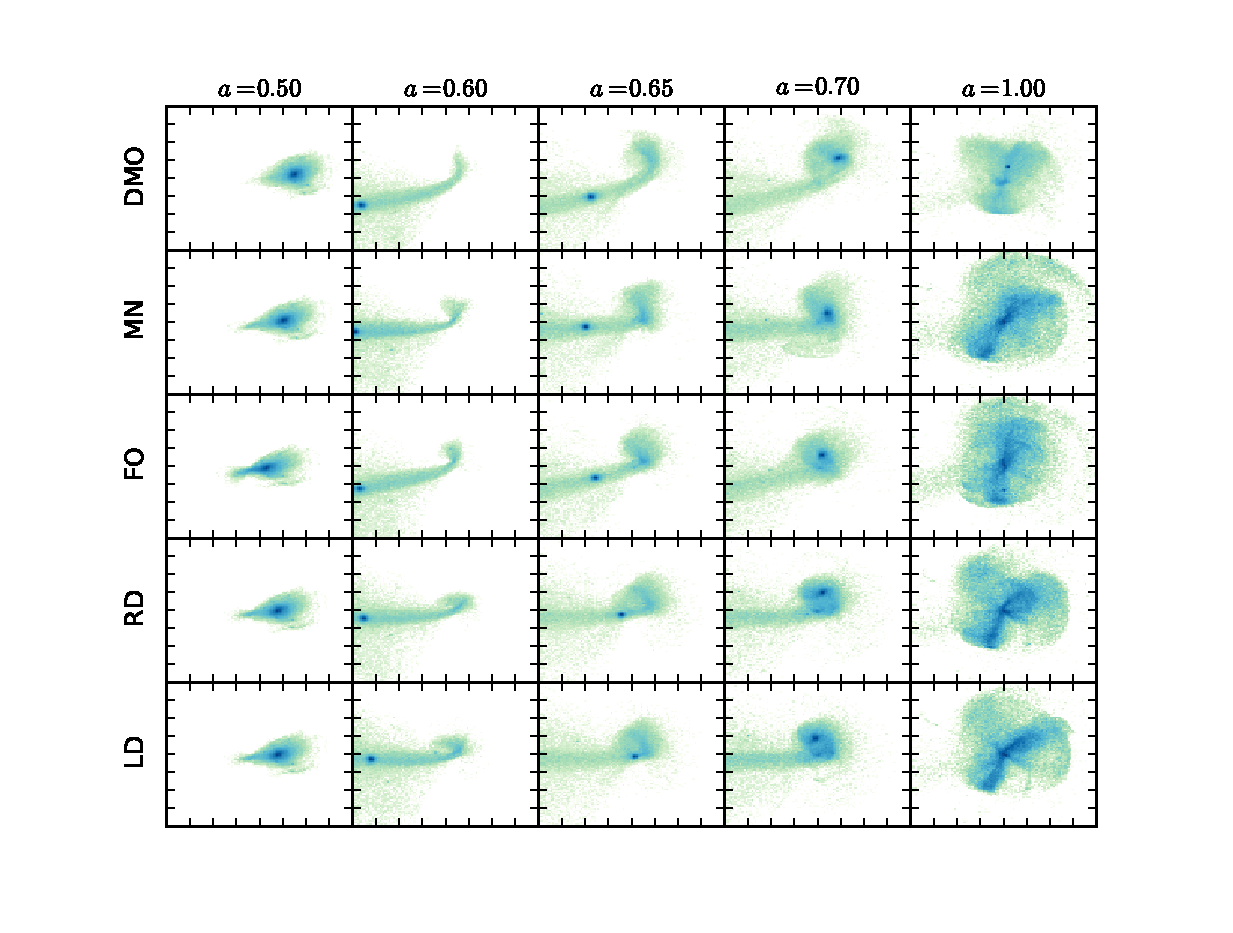
\includegraphics[width=\textwidth]{../figures/streams_side_by_side_five_sims}
\caption{X-Y projections for a selected Sagittarius-like dwarf galaxy. The
  rows from top to bottom are no disc, a fixed Miyamoto-Nagai disc, a
  rigid disc, and a live disc. The scale factors in columns from left
  to right are 0.5, 0.55, 0.6, 0.65, and 0.7. The frame edges are
  $295\,{\rm kpc}$ on each side.}\label{fig:streams}
\end{figure}

Observations of the Milky Way's dwarf galaxies and associated tidal
streams provide a potentially powerful probe of the Galactic potential
and thus the Galaxy's dark halo.  One of the best-studied examples is
the Sagittarius dwarf \citet{ibatadiscovery}.  Fortunately, our
simulation has a satellite galaxy with similar properties, namely, a
dark matter mass of $1.8 \times 10^{10} \, M_\odot$ at
$z=1.0$ and an orbit that takes it close to the disc.  We identify
this object in the five simulations using the \textsc{rockstar}
halo catalogues.  We then gather a list of IDs for all the
bound particles at an early time before the dwarf is disrupted and
follow these same particles in later snapshots using a binary
search tree look-up scheme.  In Fig.\,\ref{fig:streams} we show the
evolution of this subhalo between redshift $z_l=1$ and $z=0$. The
first row shows the baseline evolution in our
DMO simulation.  The dwarf develops leading and trailing tidal tails
during the first few billion years.  By the present epoch, the tidal
debris has dispersed throughout the halo.

The next four rows show the same satellite in our disc simulations.
Perhaps the most noticeable result is that there are stronger features
in the tidal debris at the present epoch once a disc is included.  The
detailed morphology of the tidal debris is certainly different from
one disc simulation to the next.  By eye, debris in MN and FO look
somewhat similar as does the debris in RD and LD. Perhaps the most
noticeable result is that the tidal debris extends to larger galactocentric
radii when a disc is included. The detailed morphology of the tidal debris
clearly depends on the disc insertion method. By eye, tidal debris appears
more isotropic in MN and FO than in RD and LD. The implication is that fixed
potentials are more efficient at disrupting massive satellites than a 
potential which can respond to the satellite's presence.  However, we have
only a single example of massive satellite disruption, and we caution that 
more examples of this behaviour are needed to test this hypothesis.

%\textbf{
%We emphasize that we have only
%looked at one satellite, and that it is unwise to assume that there will
%always be noticeable differences in the disruption patterns.  However, it is
%worth noting that the plausibility of non-equilibrium effects is still a relevant
%conclusion for the direction of debris studies.}

\section{Conclusions}

Simulations in which a stellar disc is inserted ``by hand" into a
cosmological N-body halo provide a compromise between simulations of
isolated disc-halo systems and cosmological simulations that include
gasdynamics and star formation.  Our method builds on the scheme
used by \citet{BerentzenShlosmanStellarDisks,DeBuhrStellarDisks} and refined by \citet{YurinSpringelStellarDisks}.  The basic idea is to introduce, at a redshift $z_g$,
a rigid disc with zero mass into a halo within a cosmological zoom-in
simulation.  Between $z_g$ and $z_l$ the disc is treated as an external
potential with a mass and size that increase adiabatically to their
present day values.  At $z_l$, the rigid disc is replaced by an N-body
one and the simulation proceeds to the present epoch with live disc
and halo particles.


Our method improves upon previous ones in two important ways.  First,
during the growth phase ($z_g > z > z_l$) the position and orientation
of the disc evolve according to the standard equations of rigid-body
dynamics.  Thus, the disc in our scheme receives its linear and angular
momentum with the halo in a self-consistent fashion and is therefore
able to move, precess, and nutate due to torques from the halo.  While
previous methods introduced aspects of rigid-body dynamics during the
growth phase none appear to have implemented the full dynamical
equations have done here \citep{DOhngiaSubstructureDepletion, DeBuhrStellarDisks, YurinSpringelStellarDisks}.

Our sequence MN, FO, RD, and LD of simulations highlights where the
details of the disc insertion scheme are important and where they are
not.  For example, schemes in which the disc tracks the minimum of the
halo potential tend to overestimate the effects of adiabatic
contraction.  On the other hand, the effect of the depletion of halo
substructure seems to be rather insensitive to the details of how the
disc is introduced into the simulation.


Disc insertion schemes such as the one introduced in this paper,
provide an attractive arena for
studies of galactic dynamics. In particular, they allow one to study the interaction between a stellar disc and a realistic dark halo with computationally inexpensive simulations while maintaining some level of control over the structural parameters of the disc.  We fully intend to leverage these advantages in future work.


\section*{Appendix A: Euler's Equations in Comoving Coordinates} \label{sec:derivation}

The time-evolution of the angular momentum vector ${\bf L}$ of a rigid
body acted upon by a torque $\boldsymbol{\tau}$ is given by

\begin{equation}
  \left(\frac{{d} \bf{L}}{{d} t}\right)_f = \left(\frac{{d} \bf{L}}{{d} t}\right)_b  + \boldsymbol \omega \times \bf{L}
  = \boldsymbol{\tau}
\end{equation}

\noindent where the subscripts $f$ and $b$ denote the frame of the
simulation box and the body frame, respectively.  In physical
coordinates, ${\bf L} = {\bf r \times p}$.  Alternatively, we can
write ${\bf L} = {\bf s\times q}$ where ${\bf s} = a^{-1}{\bf r}$
refer to comoving coordinates and ${\bf q} = a^2\dot{\bf s}$ is the
conjugate momentum to ${\bf s}$ (see \citet{QuinnIntegrators}).

For a rigid body, the components of the angular momentum are given by $L_i = I_{ij} \omega_j$ where $i,j$ run over $x,\,y,\,z$ and there is an implied sum over $j$.  Since \textsc{gadget-3} uses comoving coordinates, we write $I_{ij} = a^2 J_{ij}$ where $J$ is the moment of inertia tensor written in terms of the comoving coordinates, ${\bf s}$, rather than the physical coordinates, ${\bf r}$.  For convenience, we define a ``comoving'' angular velocity $\boldsymbol{\varpi} = a^{-2}\boldsymbol{\omega}$.  We then have $L_i = J_{ij} \varpi_j$.  Note that because of the symmetry of our disc, the moment of inertia tensor is diagonal with $J_{xx} = J_{yy}= J_{zz} \equiv J/2$.  The equations of motion for the Euler angles and the disc angular velocity are then given by the standard Euler equations of rigid body dynamics, modified to account for the time-dependence of the disc's moment of inertia:

\begin{equation}
\frac{d\phi}{dt} = a^{-2}\sin^{-1}{\theta} \left (\varpi_x\sin(\psi) + \varpi_y \cos(\psi)\right )~,
\end{equation}
\begin{equation}
\frac{d\theta}{dt} = a^{-2}\left (  \varpi_1\cos(\psi) - \varpi_y \sin(\psi)\right )~,
\end{equation}
\begin{equation}
J\frac{\varpi_x}{dt} + \varpi_x\frac{dJ}{dt}
+ J\varpi_y\varpi_z
=  \tau_x~,
\end{equation}
and
\begin{equation}
\frac{\varpi_y}{dt} + \varpi_y\frac{dJ}{dt}
- J\varpi_x\varpi_z
=  \tau_y~.
\end{equation}

\noindent We have omitted the equations for $\psi$ (rotations in the body frame about the symmetry axis) and $\varpi_z$ since these are determined directly from Eq.\,\ref{eq:omega3}.   
%\def \last_written_page{\thepage}
\bibliographystyle{apalike}
\bibliography{bibliography_paper_i.bib}
%\last_page_of_biblio
%\def \last_written_page{\thepage}

%\chapterbib


\chapter{Implementing Disc Insertion Schemes in \textsc{Gadget-3}}\label{ch:implementation}

This chapter is meant to provide more details on exactly how to implement the method described in Chapter~\ref{ch:paper_i}. Example code is included where relevant, but the author believes it is a useful exercise for a new graduate student to implement this themselves, as it tests their understanding of the material in Chapter~\ref{ch:background}. For the purposes of this guide, we are going to assume that the reader has the copy of \textsc{Gadget-3} used for this thesis and has a working understanding of how to use a compiler, MPI, and \textsc{GalactICS}.

\section{Representing a Rigid Disk}

A good deal of time was spent in the early development of the disc insertion scheme thinking about the best way to represent the rigid disc during the growth phase. There were two main approaches we considered. 

The first was to not represent the disc as a physical object in the simulation, but simply as a smooth potential.  In order to compute forces on such an object, one has to rely on Newton's third law. The force (torque) on the disc is equal and opposite to the force (torque) it exerts on every other particle in the simulation. The primary issue with this is that in a tree code or particle mesh code, Newton's third law is violated \citep{barnes_hut, hernquist_1991, GadgetCodePaper}. Furthermore, there is straightforward way to impose periodicity. Since this object exists outside of the tree or particle mesh calculations, it is not accounted for when \textsc{Gadget-3} imposes periodic boundaries.

The second approach, and the one that we used, was to represent the disc as a series of massive particles. We wanted to avoid this initially, since this opens up a wide range of potential problems. The first of these is that you need to explicitly turn off the drift and kick operations for the rigid particles. The segments of code portrayed in Appendix~\ref{ch:predict.c} from \texttt{predict.c} and Appendix~\ref{ch:kicks.c} from \texttt{kicks.c} handle the drift and kick shutoff for collisionless particles respectively. 

In order to initially position the disc, you have to set the initial \texttt{DISK\_X0}, \texttt{DISK\_Y0}, \texttt{DISK\_Z0} variables. The velocity is set by \texttt{DISK\_VX0}, \texttt{DISK\_VY0}, and \texttt{DISK\_VZ0} in units of physical velocity divided by the scale factor (internal simulation units). The initial Euler angles are given as \texttt{DISK\_PHI0}, \texttt{DISK\_THETA0}, and \texttt{DISK\_PSI0}. 

\subsection{Rigid Disk Initial Conditions}

To generate the initial conditions, you need to have the zoom-in snapshot with the halo you want to extract. To set up the rigid disc, we have been using the last snapshot of the zoom-in to create the disc. Using the \textsc{rockstar} positions (converted to kpc) and velocities, run the code provided in Appendix~\ref{ch:extract_halo_ascii.py}. Name the output file to be the path listed in the first line of \texttt{extpot.params}. \textbf{Make sure that the orientation for the rigid disk on the last line of this file is set to be toward the z-axis, or you will rotate the disk twice causing all sorts of bad things!}

Once the disk is finished generating, you need to merge it with the zoom-in particles. Place the unrotated disk at the origin, and the code will place the rigid disk upon initialization. You may use the C++ script I have provided in Appendix~\ref{ch:merge_ics.cpp}. This file will reassign all of the particle IDs and types, so make sure if you use this script that you do not need to preserve the old ones. Make sure \texttt{\#define append} and \texttt{\#define GADGET\_COSMOLOGY} are uncommented.

The disk position, velocity, angular position, and rate of Euler angle change are recorded in \texttt{disk\_vars.txt}. The differences in these quantities from the last timstep are recorded in \texttt{disk\_dvars.txt}. A variety of other quantities are written out into other log files that are pretty self explanatory. Appply \texttt{grep} to the code if you are unsure what a particular log file is. There should be comments.

%\textsc{Gadget-3} should now be run as described. You may occasionally run into an issue where \textsc{Gadget-3} cannot construct a tree and it keeps trying to increase the tree allocation factor.


\section{Integrating the Rigid Body Equations}




\subsection{Initial Parameters and Timestep Selection}
To integrate the disc, you need to set \texttt{RIGID\_PARTICLE\_DISK}, \texttt{ANALYTIC\_LZ}, and a value for \texttt{TULLY\_FISHER\_A}. You will also need a timestep reduction factor, \\\texttt{TIMESTEP\_REDUCTION\_FACTOR}, which reduces the timestep size for the rigid disc integration. We have found that accurately capturing the nutation behavior for the disk generally requires a lower timestep than what \textsc{Gadget-3} assigns from the acceleration.

On the topic of timesteps, you will need to force all of the disk particles into the same timestep bin. Recall how the time integration scheme was described; there is nothing preventing particles in the force tree that are all rigid disk particles from being assigned different timesteps. This is handled by the segment of code from \texttt{timestep.c} in Appendix~\ref{ch:timestep.c}.


\subsection{Integration}

The actual integration scheme is handled in \texttt{rigiddisk.c}. The functions are self-explanatory and implement routines for generating the Euler rotataion matrix. At runtime, the particles in the rigid disk have their relevant quantities (acceleration, torque, etc.) rotated into the frame where the disk axis is the $z$-axis. We solve the angular part of the disk dynamics in this frame using the implicit Euler method. For the actual timestep used in the integration method, make sure you use the time calculated in \texttt{update\_halo\_positions.c}. This is the actual time elapsed as formulated\footnote{You can check that you're using the right timestep by ensuring the total time elapsed corresponds to the time elapsed in that cosmology.}, not the drift or kick steps given for the conjugate positions and velocities. We apologize for the horrible mess that this section of code has become. Perhaps it would be instructive to write your own halo tracker.

\section{Live Disk Setup and Initial Conditions}

\subsection{Code Setup}
\subsection{Creating Live Initial Conditions}

\section{Known Issues and Pet Peeves}

\subsection{Choosing a Timestep}
\subsection{Integration Scheme}

\bibliographystyle{apalike}
\bibliography{bibliography_implementation.bib}

\chapter{Cosmological Bar Formation: Nature vs Nurture} \label{ch:paper_ii}

%\last_written_page

% Abstract of the paper
\section{Abstract}

We investigate the connection between the vertical structure of
stellar discs and the formation of bars using high-resolution
simulations of galaxies in isolation and in the cosmological context.
In particular, we simulate a suite of isolated galaxy models that have
the same Toomre $Q$ parameter and swing amplification parameter but
that differ in the vertical scale height and velocity dispersion.  We
find that the onset of bar formation occurs more slowly in models with
thicker discs.  Moreover, thicker discs and also discs evolved in
simulations with larger force softening also appear to be more
resilient to buckling, which acts to regulate the length and strength
of bars.  We also simulate disc-halo systems in the cosmological
environment using a disc-insertion technique developed in a previous
paper.  In this case, bar formation is driven by the stochastic
effects of a triaxial halo and subhalo-disc interactions and the
initial growth of bars appears to be relatively insensitive to the
thickness of the disc.  On the other hand, thin discs in cosmological
halos do appear to be more susceptible to buckling than thick ones and
therefore bar strength correlates with disc thickness as in the
isolated case.  More to the point, one can form discs in cosmological
simulations with relatively weak bars or no bars at all provided the
discs as thin as the discs we observe and the softening length is
smaller than the disc scale height.


\section{Introduction}

The problem of bar formation in disc galaxies tests our understanding
of cosmological structure formation and galactic dynamics.  In
principle, theories of galaxy formation should yield predictions for
the fractional distribution of bars in terms of their strength,
length, and pattern speed.  While it is often difficult to make
precise, quantitative statements about bars from observations, general
properties of their distribution have emerged (See
\citet{sellwood1993}, \citet{Sellwood2013} and \citet{BT} for
reviews).  Roughly 30-40 per cent of disc galaxies exhibit strong
bars, that is bars that dominate the disc luminosity.  Another 20 per
cent or more have relatively weak bars.  The bar fraction appears to
increase with time.  Approximately one tenth of disc galaxies between
$0.5 \le z \le 2$ have visually identifiable strong bars, which is a
factor of 3-4 smaller than the fraction in the local Universe (see
\citet{simmons2014} and references therein).  The bar fraction also
varies with galaxy type.  \citet{masters2010} find that $70\pm 5$ per
cent of the so-called passive red spirals have bars as compared to a
$25\pm 5$ per cent bar fraction for blue spirals.  Since the red
spirals are interpreted as old galaxies that have used up their
star-forming gas, this result is consistent with a bar fraction that
increases with time.  The upshot of these observations is that in
terms of bars, disc galaxies in the local Universe divide into three
roughly equal bins: those with strong bars, those with weak bars, and
those with no detectable bar.  These observations suggest that bars are 
capable of forming at a wide range of cosmic times, but once formed,
are difficult to destroy.

Intuition tells us that properties of a bar should depend on the
properties of its host galaxy and the environment in which that
galaxy lives.  Theoretical arguments indicate that cold, thin discs
are susceptible to local ``Toomre'' instabilities.  Furthermore, discs
that are strongly self-gravitating, that is discs that contribute the
bulk of the gravitational force required to maintain their rotational
motion, are susceptible to global instabilities.  Thus, one can
construct initially axisymmetric galaxy models that form bars with
vastly different properties (or no bars at all) by changing the
internal disc dynamics or trading off disc mass for bulge and halo
mass.  The implication is that the distribution of bars provides an
indirect means for inferring a disc's kinematics and mass-to-light
ratio as well as the distribution of mass in a galaxy's dynamically
``hot'' components, namely its bulge and dark matter halo.

A galaxy's ability to resist local instabilities is typically
expressed in terms of the (kinetic) Toomre $Q$-parameter
\citep{ToomreParameter} while its ability to resist global
instabilities is encapsulated in the swing-amplification $X$-parameter
\citep{GoldreichTremaine1978,GoldreichTremaine1979}.  Both parameters
are defined so that large values imply a more stable disc.  The
hypothesis that they determine a galaxy's susceptibility to bar
formation has been tested by simulations of isolated, idealized galaxy
models \citep{PeeblesOstriker1973, ZangHohlBars1978,
  CombesSandersBars1981,Sellwood1981}.  Typically, the initial galaxy
is represented by an N-body (Monte Carlo) realization of an equilibrium solution to
the collisionless Boltzmann equation comprising a disc, dark matter
halo, and often, a bulge.  Equilibrium does not imply
stability, and a galaxy can develop spiral structure and a bar through
instabilities that are seeded by shot noise
\citep{EfstathiouShotNoise} and amplified by feedback loops such as
swing amplification \citep{Sellwood2013}. A common way to suppress the mechanisms
which give rise to these effects is by increasing either $Q$ or $X$.  For
example, in dynamically warm discs (that is, discs with high $Q$)
perturbations are randomized on timescales short enough to prevent the
feedback loop from starting \citep{AthanassoulaSellwood1986}.
Likewise, submaximal discs, that is, discs with high $X$, avoid the
bar instability presumably because the disc lacks the self-gravity to
drive the bar instability \citep{EfstathiouShotNoise,
  ChristodoulouStability1995, Sellwood2013}.

As one might imagine, the parameters $Q$ and $X$ do not uniquely
describe a galaxy's susceptibility to bar formation.
\citet{WPDGalactICSReference} present a grid of models in the $Q-X$
plane that all satisfy observational constraints for the Milky Way.
These simulations confirm the basic notion that susceptibility to
instabilities increases with decreasing $Q$ and $X$.  However, a
careful study of bar strength and length as a function of time across
these simulations suggests a more complicated picture.  In particular,
the bar strength is not a perfectly monotonic function of $X$ at fixed
$Q$ or vice versa.  The implication is that additional parameters are
required to fully predict how bar formation will proceed from some
prescribed initial conditions.  In short, bar formation may
proceed very differently within a family of models that have the same
$Q$ and $X$ but vary in other ways.

One property of a disc not captured by either $Q$ or $X$ is its
thickness, or alternatively, its vertical velocity dispersion.  (The
Toomre parameter depends only on the radial velocity dispersion.)
\citet{Klypin2009} use a suite of simulations to demonstrate that the
thickness of the disc plays a profound role in the development of a
bar.  In particular, their thick disc model forms a stronger and more
slowly rotating bar as compared with the bar that forms in a thin disc
model with the same initial radial dispersion profile and rotation
curve decomposition.  Moreover, simulation parameters such as mass
resolution and time step also influence the growth of the bar
instability and slowdown of the bar due to angular momentum transfer
with the dark halo \citep{dbs2009}.

Of course, galaxies are neither isolated nor born as axisymmetric,
equilibrium systems. In these idealized systems, instabilities can only come from shot noise, whereas this is is not true in a complicated dynamical environment. As such, bar formation may be very different in idealized
galaxies as compared with galaxies in a cosmological setting.  For
example, halo substructure in the form of satellite galaxies and dark
matter subhaloes can pass through and perturb the disc.
\citet{gauthier2006}, \citet{kazantzidis2008}, and
\citet{dbs2009} showed that an apparently stable disc galaxy
model can develop a bar when a fraction of the ``smooth'' halo is
replaced by substructure in the form of subhaloes.  The effect is
stochastic; subhalo-triggered bar formation seems to require subhaloes
whose orbits take them into the central regions of the disc in a
prograde sense.  More recently, \citet{purcell2011} showed that
Sagittarius dwarf alone could have been responsible for the Milky
Way's spiral structure and bar.

Cosmological haloes also possess large-scale time-dependent tidal
fields, which impart torques to the disc and cause it to precess,
nutate, and warp
\citep{dubinski1995,binney1998,dubinski2009,Bauer2018a}.  In turn,
stellar discs can reshape the inner parts of the dark matter haloes
via adiabatic contraction and dynamical friction
\citep{blumenthal1986, ryden1987, dubinski1994,
  DubinskiKuijkenRigidDisks,
  DeBuhrStellarDisks,YurinSpringelStellarDisks, Bauer2018a}.  In
principle, one can turn to {\it ab initio} hydrodynamic cosmological
simulations to capture the effects of both triaxiality and
substructure.  Indeed, galaxy formation studies in the cosmological
environment that include the formation of supermassive black holes,
stars, and the feedback from these objects on galaxy formation have
had remarkable success over the last decade (See, for
  example \citet{IllustrisFeedback, Eagle}).  Unfortunately, feedback
techniques are extremely computationally expensive.  Moreover, the
simulator cannot control the properties of the disc such as its mass
and radial scale length that form within a particular haloes.  This
restriction makes it difficult to explore the ``nature vs. nurture''
question: Do bars reflect the structure of their host galaxy,
substructure interactions of the disc's lifetime, or large-scale tidal
fields from the dark halo?

Techniques developed by \citet{BerentzenShlosmanStellarDisks},
\citet{DeBuhrStellarDisks}, \citet{YurinSpringelStellarDisks},
\citet{Bauer2018a} and others allow one to insert a collisionless disc
into a dark matter halo.  These techniques provide a compromise
between fully cosmological simulations and simulations of isolated
galaxies.  In general, the first step is to run a pure dark matter
simulation of a cosmological volume and select a halo suitable for the
galaxy one intends to study.  The simulation is then rerun with a rigid
disc potential that is adiabatically grown from some early epoch (say
redshift $z=3$) and an intermediate one (say $z=1$).  Doing so allows
the halo to respond to ``disc formation''.  At the intermediate
redshift, a suitable N-body disc that is approximately in equilibrium
is swapped in for the rigid disc potential and the simulation
continues, now with live disc and halo particles.

Perhaps the most striking and perplexing result to come from recent
disc-insertion simulations is the prevalence of strong bars.
\citet{YurinSpringelStellarDisks}, for example, find that all of the
discs in their bulge-less simulations for strong bars even though some
of these discs are decidedly submaximal.  In addition, over half of
the discs in simulations with classical bulges form strong bars.
Their results suggest that discs in the cosmological setting are more
prone to forming strong bars and that bulges play an essential role in
explaining the presence of disc galaxies with weak bars or no bars at
all.

Though the \citet{YurinSpringelStellarDisks} models vary in $Q$ and
$X$ they share two important properties.  First, the ratio of the
radial and vertical velocity dispersion is set to unity throughout the
disc.  Second, the ratio of the vertical and radial scale lengths is
fixed at $0.2$, which is roughly a factor of two larger than that of
the Milky Way's thin disc.  In addition, the softening length in their
simulations is fixed at $680\,{\rm pc}$.  Thus, the discs in their
simulations are thicker and (vertically) warmer than what one might
expect for Milky Way-like galaxies.  The results from
\citet{Klypin2009} suggest that these properties rather than (or
together with) halo substructure and triaxiality are responsible for
the preponderance of strong bars in the
\citet{YurinSpringelStellarDisks} models.

In this paper, we attempt to isolate the different effects that
determine whether a galaxy forms a strong bar, a weak one, or no bar
at all.  The core of the paper is a a sequence of N-body simulations
that include simulations of isolating disc galaxies and galaxies in
cosmological haloes.  Our choice of models is meant to complement
those of \citet{YurinSpringelStellarDisks}.  In particular, we choose
models that have the same $Q$ and $X$ but that vary in 
their vertical structure.  

We begin in section \S \ref{sec:ics} by discussing the dimensionless
parameters that arise when one constructs equilibrium disc galaxy
models.  These include the aforementioned $Q$ and $X$ parameters as
well as the ratio of the vertical and radial velocity dispersion and
the ratio of the vertical and radial scale lengths.  We also discuss
possible effects of gravitational softening.  In
\ref{sec:thick_discs_suppress} we describe our sequence of simulations
and discuss how they fit in with previous work.  We discuss results
for our isolated galaxy simulations in \S \ref{sec:isolated} and our
cosmological ones in \S \ref{sec:cosmo}.  We conclude with a
discussion of the implications of our results in \S
\ref{sec:conclusions}.

\begin{figure}
	\centering
	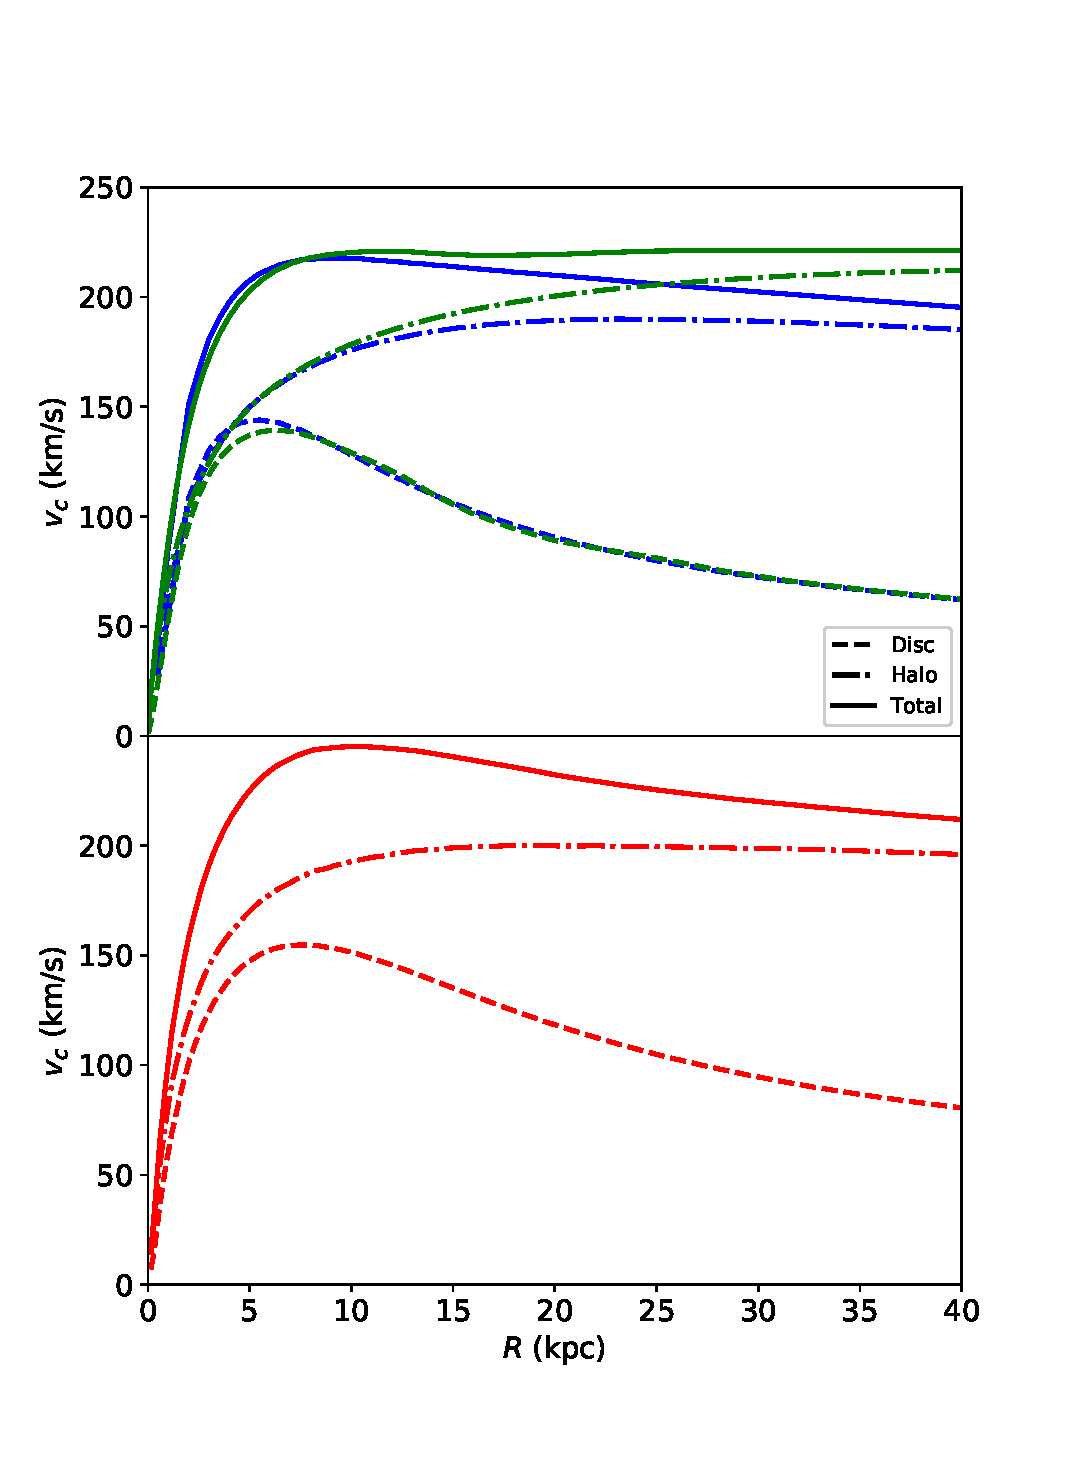
\includegraphics[width=0.9\textwidth]{../figures/rotation_curves_two_panel.eps}
	\caption{Rotation curve decomposition for our models. Total
          rotation curves are shown as solid lines while the separate
          contributions from the disc and halo are shown as dashed and
          dot-dashed curves, respectively.  Blue curves in the top
          panel are for the isolated galaxy simulations with
          \textsc{GalactICS} initial conditions while the green curves
          are for the simulations C.I.Ag run with \textsc{AGAMA}
          initial conditions.  Bottom panel shows initial rotation
          curve decomposition for the runs D.I and
          E.II.}\label{fig:rcs}
\end{figure}

\begin{table*}
\begin{tabular}{l l l l l l l l l l l l}
\hline
 & $M_d$ & $R_d$ & $V_c$ & $\sigma_R$ & $z_d/R_d$  & $\sigma_R/\sigma_z$  & $X$ &  $Q$ & $\rho_h/\rho_0$ & $\epsilon$ \\ 
\hline
A.I     & 3.49 & 2.50 & 216 & 25.3 & 0.10 & 1.27 & 2.34 & 1.00 & 0.14 & 0.15\\
A.II    & 3.49 & 2.50 & 216 & 25.3 & 0.10 & 1.27 & 2.34 & 1.00 & 0.14 & 0.50\\
B.I     & 3.49 & 2.50 & 213 & 25.3 & 0.20 & 0.97 & 2.34 & 1.00 & 0.28 & 0.15\\
B.II    & 3.49 & 2.50 & 213 & 25.3 & 0.20 & 0.97 & 2.34 & 1.00 & 0.28 & 0.50\\
C.I     & 3.49 & 2.50 & 208 & 25.3 & 0.40 & 0.77 & 2.34 & 1.00 & 0.50 & 0.15\\
C.I.Ag  & 3.49 & 2.50 & 216 & 25.3 & 0.40 & 0.77 & 2.34 & 1.00 & 0.50 & 0.15\\
D.IV    & 5.82 & 3.70 & 245 & 25.2 & 0.10 & 1.14 & 2.45 & 1.00 & 0.29 & 0.18\\
E.IV    & 5.82 & 3.70 & 245 & 27.4 & 0.25 & 0.72 & 2.45 & 1.00 & 0.73 & 0.74\\
\hline
YS15.A5 & 5.00 & 3.00 & 263 & 30.7  & 0.2 & 1.00 & 3.22 & 1.38 & 0.21 & 0.68\\
YS15.B5 & 5.00 & 3.00 & 211 & 26.6  & 0.2 & 1.00 & 2.06 & 0.96 & 0.11 & 0.68\\
YS15.C5 & 5.00 & 3.00 & 270 & 30.3  & 0.2 & 1.00 & 3.31 & 1.42 & 0.23 & 0.68\\
YS15.D5 & 5.00 & 3.00 & 236 & 26.6  & 0.2 & 1.00 & 2.58 & 1.12 & 0.16 & 0.68\\
YS15.E5 & 5.00 & 3.00 & 233 & 27.1  & 0.2 & 1.00 & 2.58 & 1.11 & 0.15 & 0.68\\
YS15.F5 & 5.00 & 3.00 & 219 & 27.0  & 0.2 & 1.00 & 2.22 & 1.02 & 0.11 & 0.68\\
YS15.G5 & 5.00 & 3.00 & 227 & 28.2  & 0.2 & 1.00 & 2.45 & 1.09 & 0.13 & 0.68\\
YS15.H5 & 5.00 & 3.00 & 244 & 28.6  & 0.2 & 1.00 & 2.85 & 1.21 & 0.16 & 0.68\\
\hline
G06     & 7.77 & 5.57 & 226 & 17.1  & 0.06  & 1.80 & 2.78 & 1.43 & 0.10 & 0.15 \\
\hline
%$M_d$ & $7.2 \times 10^{10} M_\odot$\\
%$N_d$ & $10^6$\\
%$R_{d,0}$ & 3.7 kpc\\
%$N_{r}$ & $4096^3$
\end{tabular}
\caption{Summary of parameters for the simulations considered in this
  paper, the disk-halo simulations considered in
  \citet{YurinSpringelStellarDisks} (labeled YS15) and the
  \citet{gauthier2006} (G06).  $M_d$ is the final disc mass in units of
  $10^{10}\,M_\odot$ , $R_d$ is the disc scale radius in units of
  ${\rm kpc}$, and $V_c$ and $\sigma_R$ are the circular speed and
  radial velocity dispersion in units of ${\rm km\,s^{-1}}$ and
  evaluated at $R_p = 2.2R_d$.  For the disc aspect ratio, we quote
  $z_d/R_d$ where $z_d$ is the ${\rm sech}^2$-scale length.  The
  velocity dispersion ratio $\sigma_R/\sigma_z$, the $X$ and $Q$
  parameters, the ratio of the halo density in the midplane to that of
  the disc, and the logarithmic derivative of the circular speed are
  also measured at $R_p$.  Finally, the softening length $\epsilon$ is
  given in units of ${\rm kpc}$.  Simulations A.III and B.III are the
  same as A.I and B.I except that they are run with vertical motions
  isotropized so as to shut off the buckling
  instability.} \label{tab:sims}
\end{table*}

\section{Theoretical Considerations}
 \label{sec:ics}

In this section, we consider the structural properties of disc-halo
models with an eye toward understanding the formation of bars in these
systems.  We begin with the $Q$ and $X$ parameters and then discuss the
vertical structure of the disc as defined by its scale height,
vertical velocity dispersion, and surface density.  Finally, we
consider the effect softening might have on bar formation.

\begin{figure}
	\centering
        \includegraphics[width=0.9\textwidth]{../figures/falpha.eps}
        \caption{The dimensionless ratio $\sigma_z^2/\pi G\Sigma z_d$ as a
          function of $\rho_h/\rho_0$ for the models considered in
          this paper (stars), the disc-halo models from
          \citet{YurinSpringelStellarDisks} (filled squares) and the
          model from \citet{gauthier2006} (filled triangle).  The
          straight line is the function $f = 1 + \left (2\pi/3\right
          )^{1/2}\rho_h/\rho_0$ discussed in the text.}
\label{fig:falpha}\end{figure}

\begin{figure*}
	\centering
        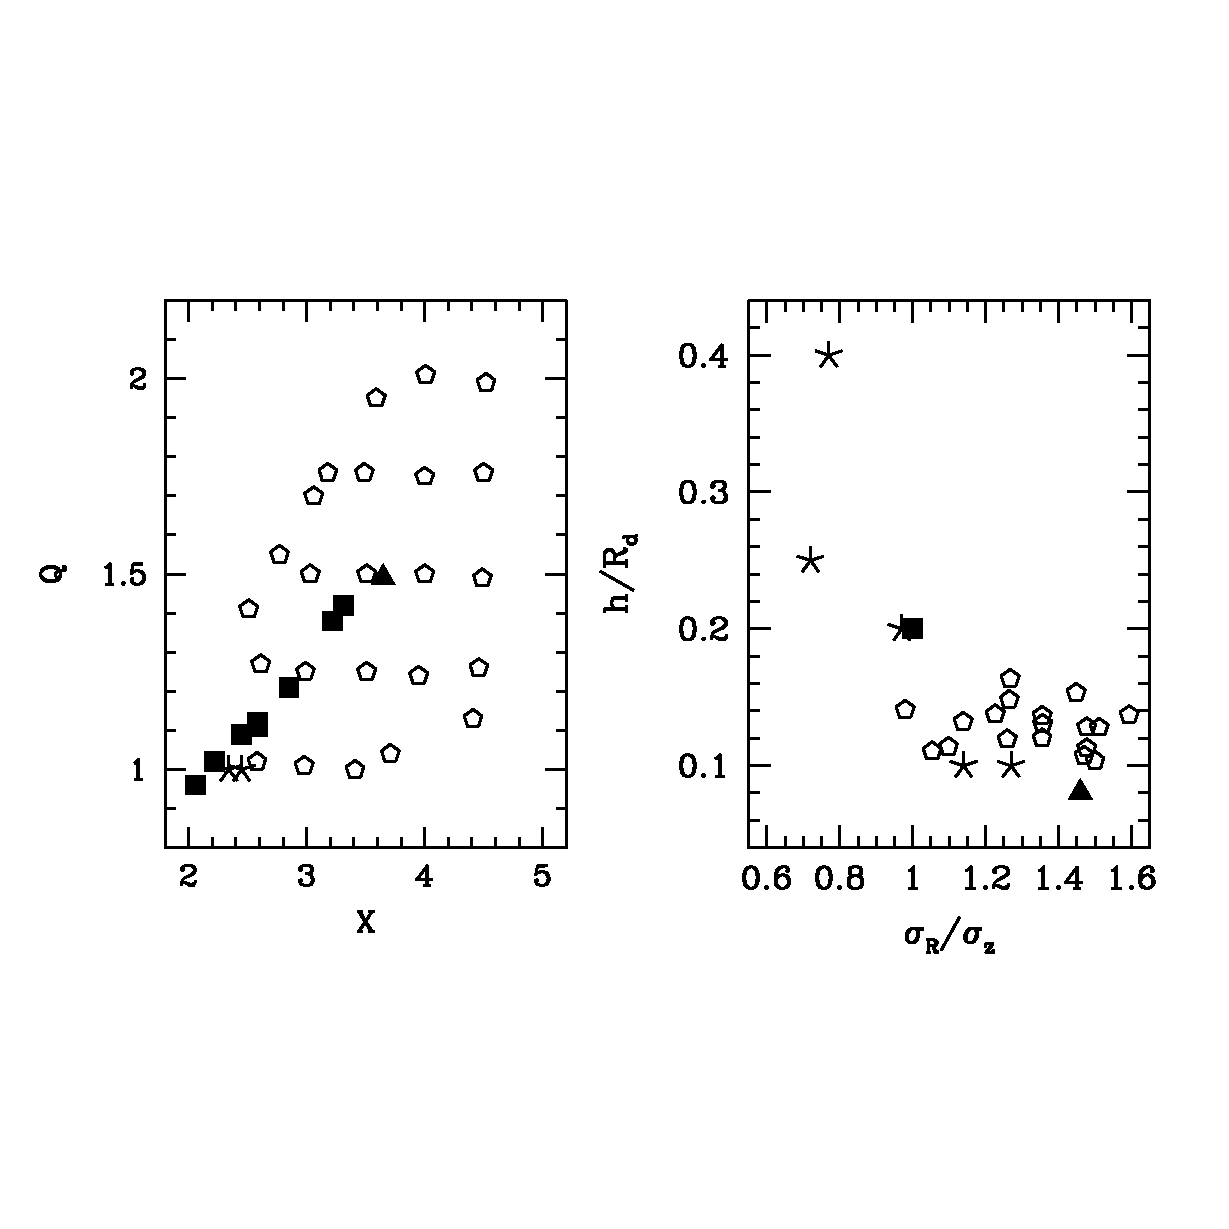
\includegraphics[width=1.\textwidth]{../figures/qxr.eps}
        \caption{Distribution of simulations considered in this paper
          in the $Q-X$ and the $z_d/R_d-\sigma_R/\sigma_z$ planes.
          Stars are simulations run for this paper (A-E); filled
          squares denote the series of simulations described in
          \citet{YurinSpringelStellarDisks}; the filled triangle denotes
          the simulation of M31 run in \citet{gauthier2006}; open
          pentagons denote the simulations described in
          \citet{WPDGalactICSReference}.
        }\label{fig:QXR}\end{figure*}


\begin{figure}
	\centering
	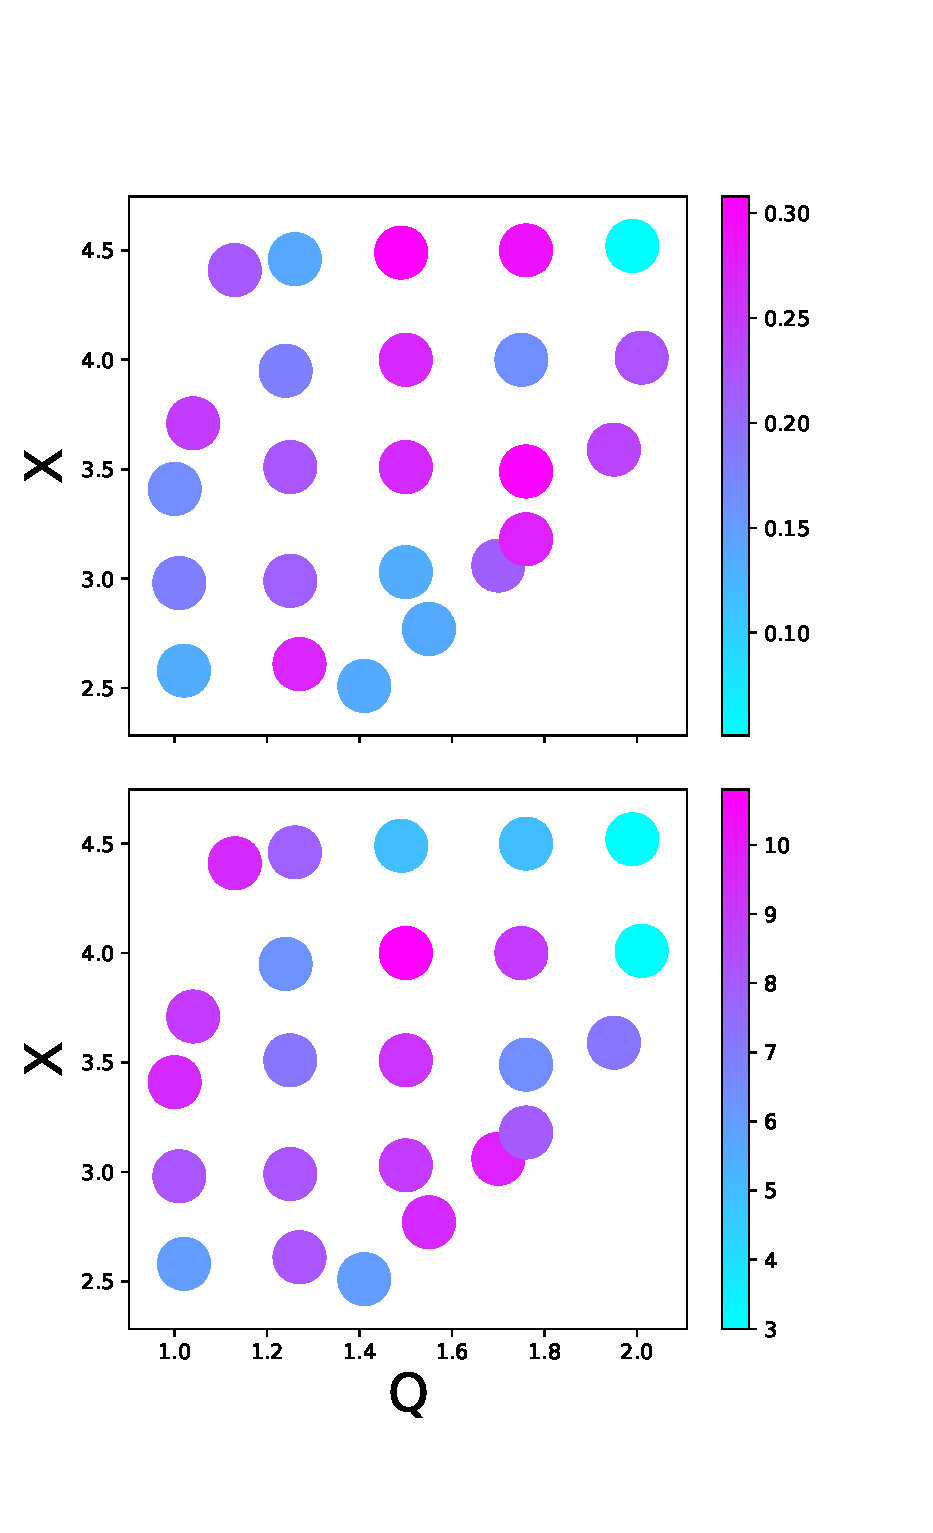
\includegraphics[width=0.75\textwidth]{../figures/wpd.eps}
	\caption{Strength and length of bars for the simulations
          considered in \citet{gauthier2006}.  The twenty-five models
          span the $Q$-$X$ plane.  Top panel shows the $A_2$ parameter
          while the bottom panel shows the bar length.  Both are
          measured at $5\,{\rm Gyr}$ (the final snapshot of the
          simulations).}
	\label{fig:qxa2}
\end{figure}


\begin{figure*}
	\centering
	\includegraphics[width=\textwidth]{../figures/isolated_xy_with_agama_with_circles.eps}
	\caption{Surface density maps for isolated galaxy simulations
          at select times. Time proceeds from 0 to 10 Gyr,
          left-to-right, and the models span top-to-bottom in order of
          their appearance in Table \ref{tab:sims}. The overlaid red
          circles have radii $R_p=5.5\,{\rm kpc}$ and 20 kpc.}
	\label{fig:face_on_isolated}
\end{figure*}

\begin{figure}
	\centering
	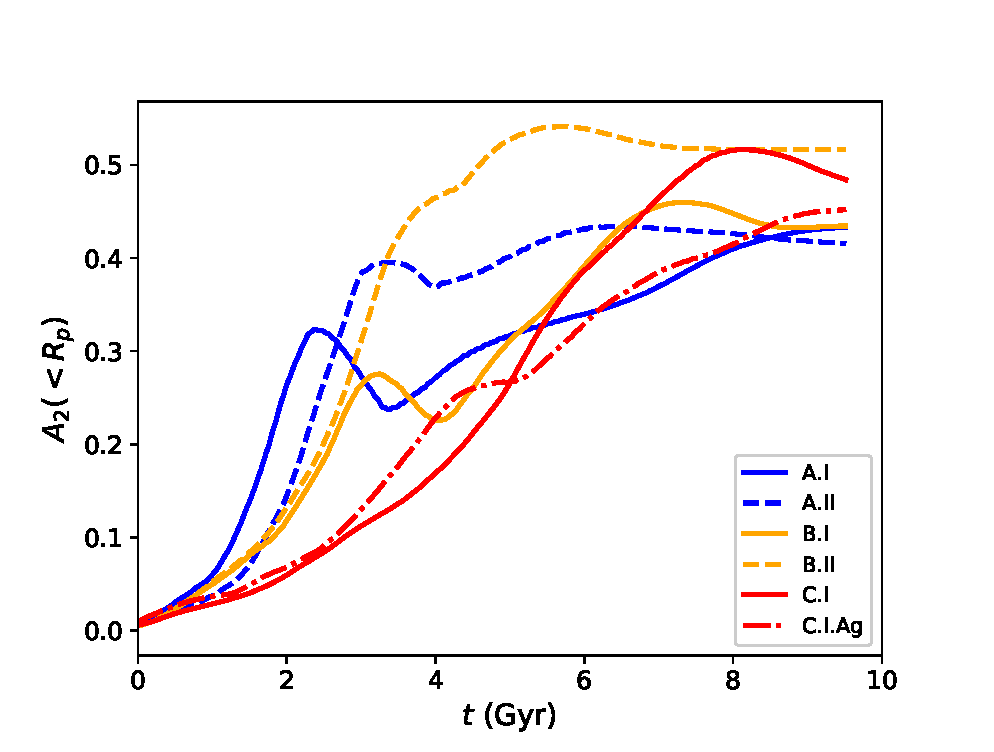
\includegraphics[width=0.9\textwidth]{../figures/isolated_a2_vs_t_2rd_weighted.eps}
	\caption{Mean bar strength parameter inside a cylindrical
          radius $R_p$, $A_2(<R_p)$, as a function of time. Curves are
          smoothed in time with a top-hat moving window of width
          $1\,{\rm Gyr}$.  Line colors are blue, red, and green for
          models A, B, and C, respectively.  Results for the
          fiducial runs A.I, B.I, and C.I are shown as solid curves
          while the results for the runs with high softening length,
          A.II and B.II, are shown as dashed curves.  The
          \textsc{AGAMA} model C.I.Ag is shown as a dot-dashed
          curve.} \label{fig:isolated_a2_vs_t}
\end{figure}

\begin{figure*}
	\centering
	\includegraphics[width=1.1\textwidth]{../figures/isolated_r_t_a2_with_agama.eps}
	\caption{Bar strength parameter $A_2$ as a function of radius
          and time.  The trajectory of corotation is shown by the
          dashed red line.} \label{fig:isolated_r_t_a2}
\end{figure*}

\begin{figure*}
	\centering
	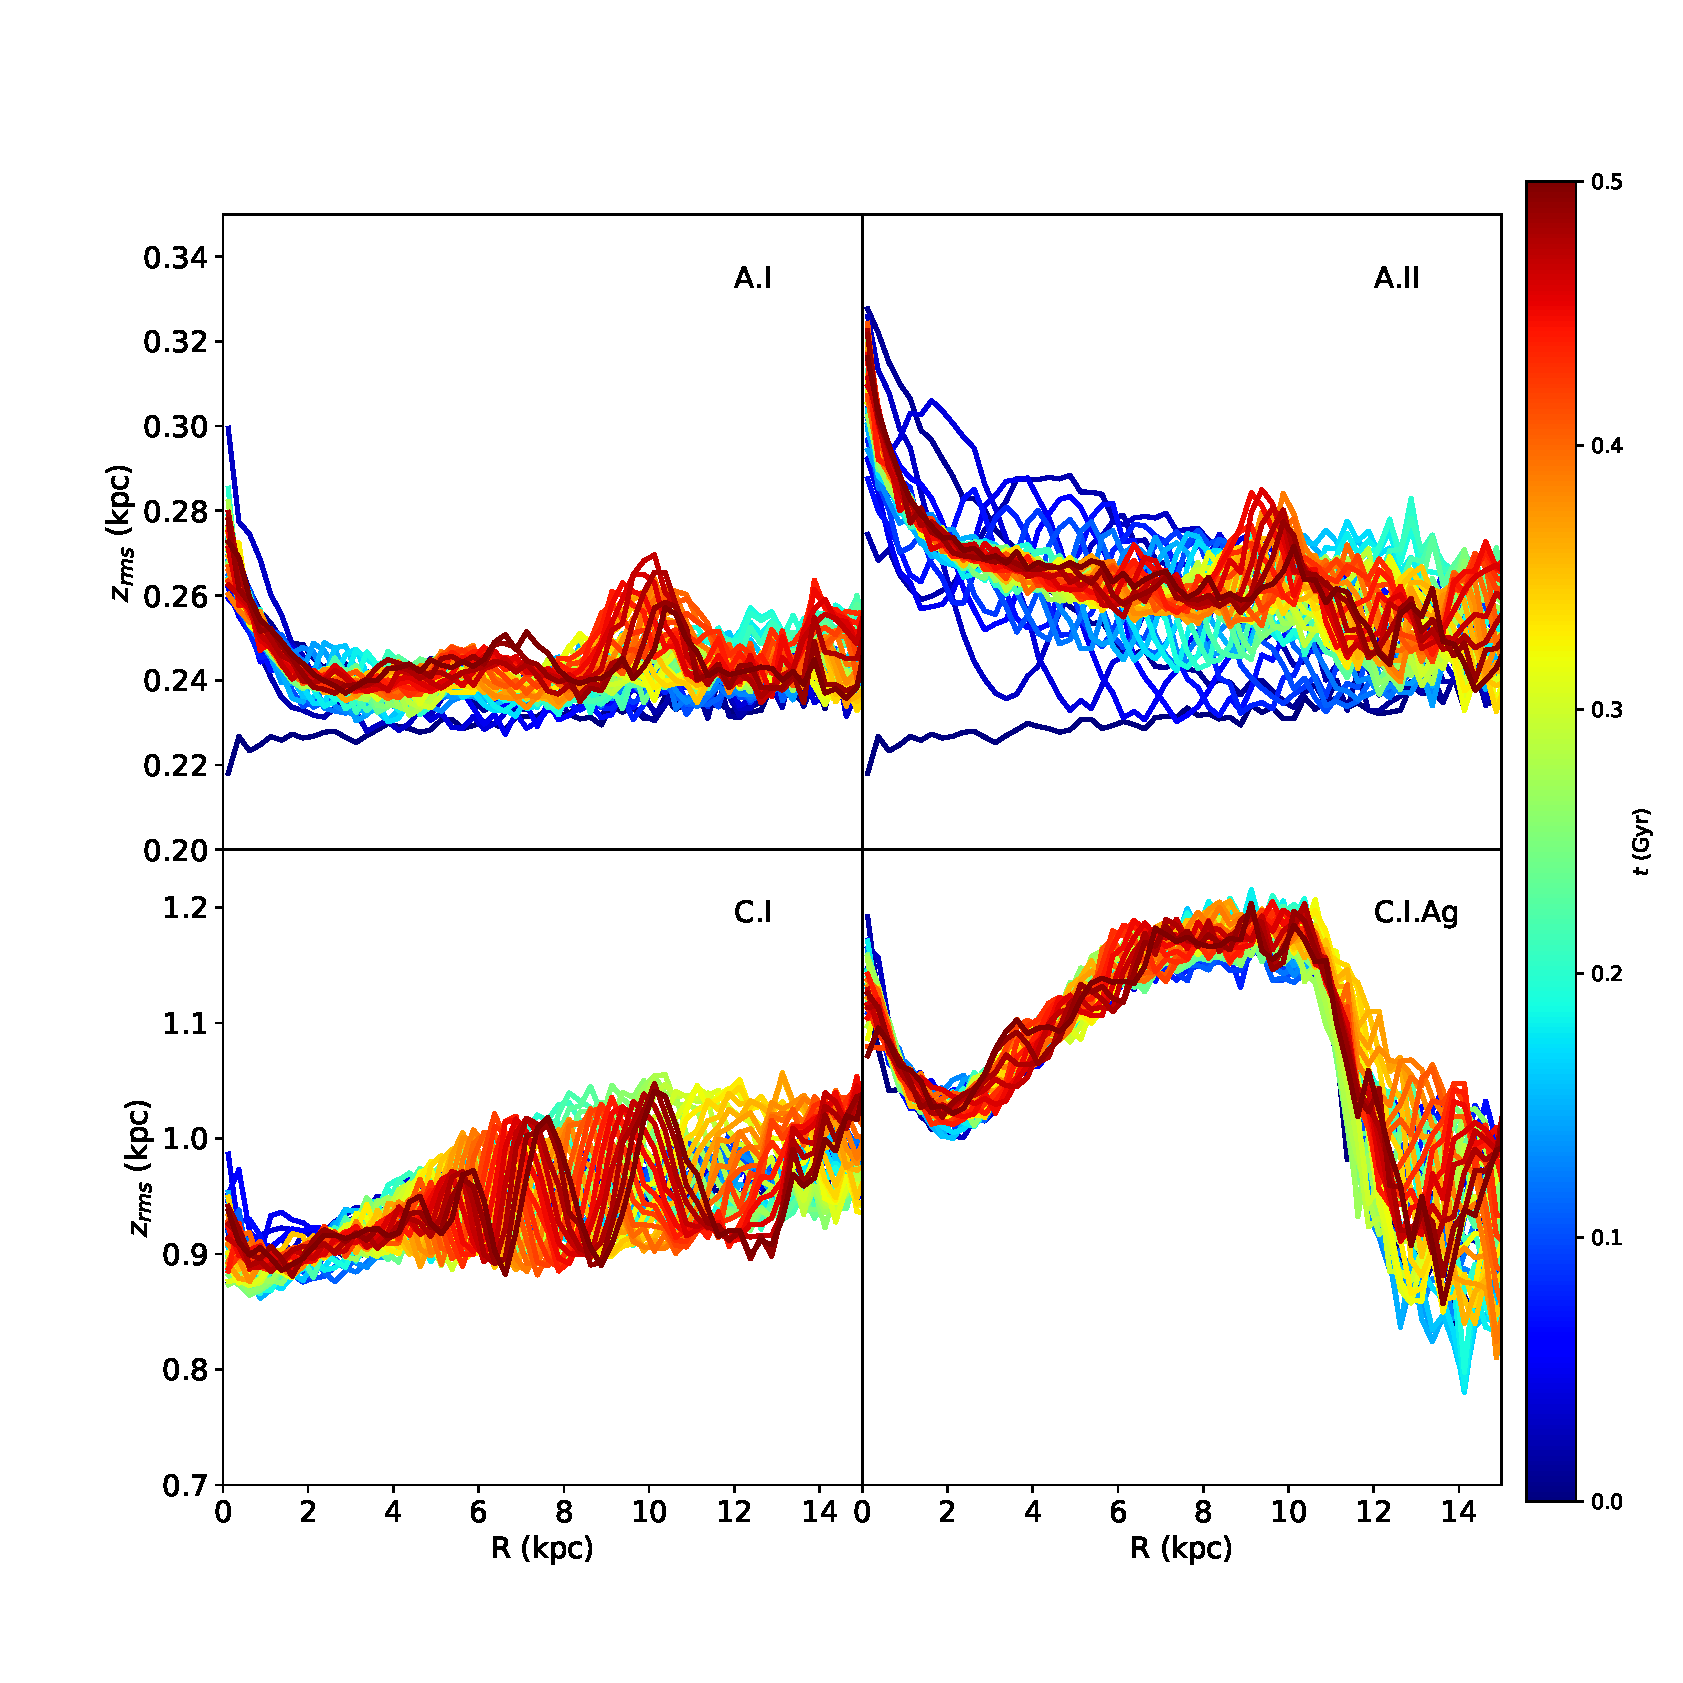
\includegraphics[width=\textwidth]{../figures/isolated_four_panel_zrms.eps}
	\caption{Root mean square height $\zrms$ as a function of
          cylindrical radius $R$ for ten snapshots equally spaced over
          the first $500\,{\rm Myr}$.  Panels are for simulations A.I
          (upper left), A.II (upper right), C.I (lower left) and
          C.I.Ag (lower right).} \label{fig:zrms}
\end{figure*}

\begin{figure*}
	\centering
	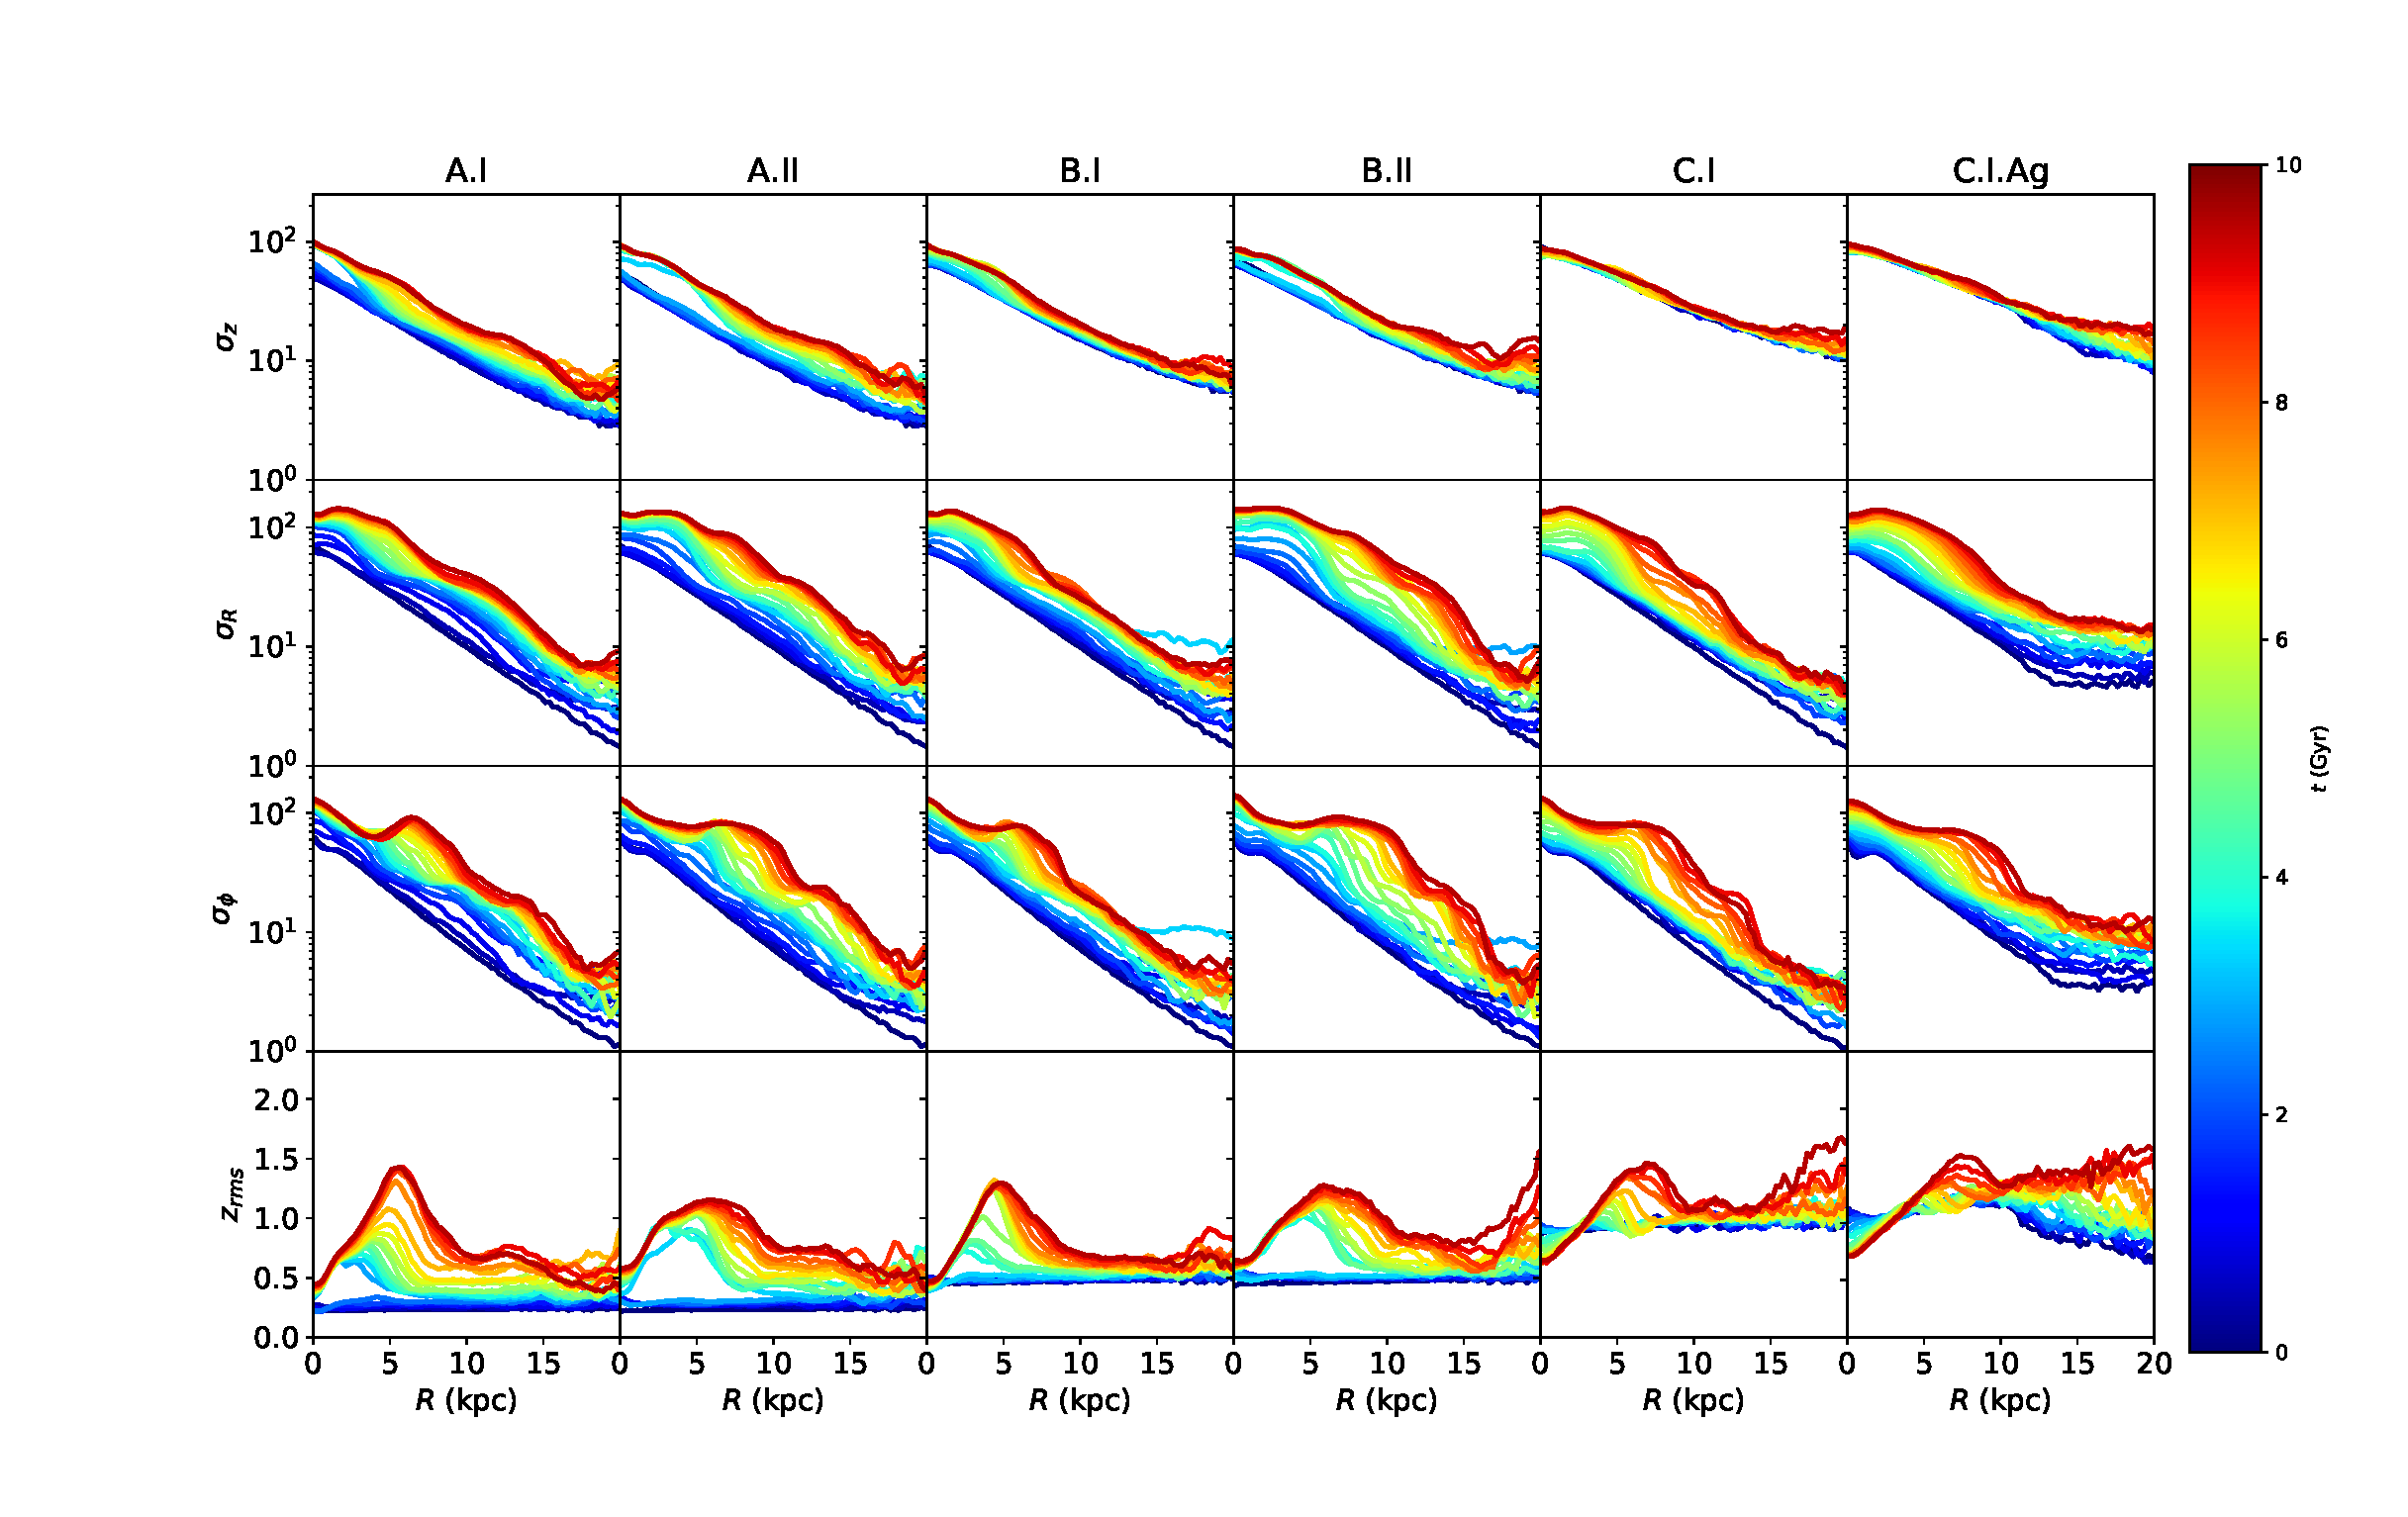
\includegraphics[width=\textwidth]{../figures/isolated_dispersion_evolution_with_agama_zrms.eps}
	\caption{Diagonal components of the velocity dispersion tensor
          and $\zrms$ as a function of $R$ for different snapshots
          between $0$ and $10\,{\rm Gyr}$.  Shown, from to to bottom,
          are profiles for $\zrms$, $\sigma_z$, $\sigma_R$, and $\sigma_\phi$
          for the same size models included in
          Fig.\,\ref{fig:face_on_isolated}.} \label{fig:isolated_dispersions}
\end{figure*}

\subsection{$Q$ and $X$} 
The stability of a stellar disc is generally thought to be determined
by the Toomre-$Q$ parameter \citep{ToomreParameter}

\begin{equation} \label{eq:q}
Q \equiv \frac{\sigma_R\kappa}{3.36G\Sigma}
\end{equation}

\noindent and the Goldreich-Tremaine (swing amplification) parameter
\citep{GoldreichTremaine1978, GoldreichTremaine1979}

\begin{equation} \label{eq:xm}
X_m \equiv \frac{\kappa^2 R}{2\pi m G\Sigma}
\end{equation}

\noindent where $R$ is the Galactocentric radius of a cylindrical
$\left (R,\,\phi,\,z\right )$ coordinate system, $\Sigma$ is the
surface density of the disc, $\sigma_R$ is the radial velocity
dispersion of the disc, and $m$ is the azimuthal mode number.  The
epicyclic radial frequency $\kappa$ is given by

\begin{equation} \label{eq:kappa2}
\kappa^2 = \frac{2V_c^2}{R^2}\left (1 + \frac{d\ln{V_c}}{d\ln R}\right )
\end{equation}

\noindent where $V_c$ is the circular speed.  We assume an exponential
disc with mass $M_d$, radial scale length $R_d$, and surface density
\begin{equation} \label{eq:sigma}
\Sigma(R) = \frac{M_d}{2\pi R_d^2} e^{-R/R_d}~.
\end{equation}
\noindent Note that $\kappa$, $\sigma_R$, $\Sigma$, $V_c$, $Q$, and
$X_m$ are functions of $R$.  In what follows, we consider the radius
$R_p$ at which the contribution to the rotation curve from the disc,
$V_d$ reaches a peak value.  For an exponential disc, $R_p \simeq
2.2R_d$ and $V_{d}(R_p) \simeq 0.62 \left (GM_d/R_d\right )^{1/2}$
\citep{BT}.

Roughly speaking, $Q$ describes the susceptibility of a disc to local
instabilities.  Cold discs with low velocity dispersion and $Q<1$ are
unstable to local perturbations.  On the other hand, $X_m$ describes
the vigour with which a global perturbation with an $m$-fold azimuthal
symmetry undergoes swing amplification.  Since we are interested in
bar formation, we set $m=2$ and note that $X_2^{-1}$ is a measure of
disc self-gravity.  To see this, we use Eq.\,(4) and the expression
for $V_{d,p}$ to find

\begin{equation} \label{eq:x2}
X_2(R_p) \simeq  0.79\,\frac{V_c^2}{V_d^2}\Biggr\rvert_{R_p}
\end{equation}

\noindent where we have assumed that the logarithmic derivative in
Eq.\eqref{eq:kappa2} is zero.

For simplicity, we define

\begin{equation} \label{eq:x}
X \equiv  \frac{V_c^2}{V_d^2}\Biggr\rvert_{R_p}~.
\end{equation}

\noindent Therefore $X=2$ when the contribution of the disc to the
circular speed curve at its peak is equal to the combined
contributions of the dynamically hot components, namely the bulge and
halo.  Following \citet{EfstathiouShotNoise},
\citet{YurinSpringelStellarDisks}, use $Q_{\rm bar} = V_{\rm
  max}/\left (GM_d/R_d\right )^{1/2}$ where $V_{\rm max}$ is the
maximum circular speed.  If we assume that $V_{\rm max}\simeq
V_c(R_p)$, then $Q_{\rm bar}^2 \simeq 0.387 X$ and the stability
criterion from \citet{EfstathiouShotNoise}, $Q_{\rm bar}>1.1$, becomes
$X > 3.13$.

\subsection{Vertical Structure of Stellar Discs}

As discussed in \citet{Klypin2009} the vertical structure of a stellar
disc plays a key role in determining the properties of any bar that
forms.  In general, the vertical structure is characterized by the
vertical velocity dispersion $\sigma_z$, surface density $\Sigma$, and
scale height.  For a self-gravitating plane-symmetric isothermal disc
these quantities are connected through the relation $\sigma_z^2 =
\sqrt{12}G\Sigma \zrms$ where $\zrms$ is the root mean square distance
of ``stars'' from the midplane.  \citep{spitzer1942, camm1950}.

We can incorportate the effects of dark matter by modifying
the Poisson equation

\begin{equation} \label{eq:spitzerpoisson}
\begin{aligned}
\frac{d^2\Phi}{dz^2} & = 4\pi G \left (\rho_d(z) + \rho_h(z) \right )\\
& = 4\pi G\rho_0 \left(e^{-\Phi/\sigma_z^2} + \rho_h/\rho_0\right )
\end{aligned}
\end{equation}

\noindent where $\rho_d$ and $\rho_h$ are the densities of the disk
and halo, respectively, and $\rho_0$ is the density of the disc in the
midplane.  In the second line we assume, as is done in the pure
self-gravitating case, that the disc stars are vertically isothermal
with velocity dispersion $\sigma_z$.  We also assume that the halo
density is constant in the region of the disc.  We then solve
Eq.\,\ref{eq:spitzerpoisson} numerically.  The result is
well-described by the relation

\begin{equation}\label{eq:sigz2}
\sigma_z^2 = \sqrt{12} 
G\Sigma \zrms \left (1 + \alpha\rho_h/\rho_0\right )
\end{equation}

\noindent where the factor $1 + \alpha = 1 + \sqrt{2\pi/3}$ provides a
simple interpolation between the pure self-gravitating case and the
case where disc particles are test particles in the (harmonic)
potential of a constant density halo.  As discussed in the next
section Eq.\,\ref{eq:sigz2} holds at the 10 per cent level for our
equilibrium models.  Departures from Eq.\,\ref{eq:sigz2} might come
from radial gradients and the rotation of the disc. (See, for example,
\citet{read2014}).

Combining Eqs.\,\ref{eq:q}, \ref{eq:x}, \ref{eq:sigz2} we find 
following relation:

\begin{equation}\label{eq:r}
\frac{Q^2}{X} = 3.103 \,
\frac{\sigma_R^2}{\sigma_z^2} \,
\frac{\zrms}{R_d}\,
f\left (1 + \frac{d\ln V_c}{d\ln R}\right )~.
\end{equation}
\noindent This expression can be interpreted in several ways.  First,
if the ratios of $\sigma_R$ to $\sigma_z$ and $\zrms$ to $R_d$ are
fixed, then there is a linear relation between $Q^2$ and $X$.  On the
other hand, if one considers a family of models in which the only
variation is in the vertical structure of the disc, then the scale
height varies roughly linearly with the vertical velocity dispersion,
apart from corrections due to the contribution of the halo to the
vertical force.

\subsection{Effect of Gravitational Softening} 

Numerical effects can significantly alter the development of bars in
simulated galaxies. For example, in simulations of an isolated galaxy
that is initially in equilibrium, the onset of bar formation is
delayed when mass resolution is increased \citep{dbs2009}
essentially because the bar instability is seeded by shot noise.  The
importance of mass resolution as well as force resolution and time
stepping are also discussed in \citet{Klypin2009}.

In this section, we focus on the effects of force softening.
Equilibrium models, such as the ones used as initial conditions in
isolated galaxy simulations, satisfy the collisionless Boltzmann and
Poisson equations.  When evolved with force softening, they will begin
slightly out of equilibrium.  This effect should be most noticeable
when the softening length is comparable to or larger than the
thickness of the disc.  To gain some intuition as to this extent of
this effect we the Poisson equation in one dimension.  The potential
for a mass distribution with vertical density profile of $\rho(z)$ can
be calculated by convolving $\rho$ with the Green's function:
\begin{equation}\label{eq:greensfunction}
\Phi(z)= 4\pi G\int_{-\infty}^{\infty} \mathcal{G}(z^\prime - z)
\rho(z^\prime) \text{d} z^\prime~.
\end{equation}
For Newtonian gravity, $\mathcal{G} = |z|/2$.  For softened gravity,
we replace $\mathcal{G}$ with $\mathcal{G}_s = \frac{1}{2}\left (z^2 +
\epsilon^2\right )^{1/2}$ where $\epsilon$ is the softening length.
(The motivation for this expression is as follows: Begin with a system
of Plummer-softened particles, that is, a system where point-like
particles are replaced by particles whose spherical density profile is
proportional to $\left (r^2 + \epsilon^2\right )^{-5/2}$.  If the
particles are confined to a plane, then the vertical density profile
will be $\rho(z)\propto \left (z^2 + \epsilon^2\right )^{-3/2}$.  The
one-dimensional potential with this $\rho(z)$ is indeed proportional
to $\left (z^2 + \epsilon^2\right )^{1/2}$.)  The integral
Eq.\,\ref{eq:greensfunction} and the related integral for the vertical
force, $f(z)$, can be evaluated numerically.  As expected, the
potential energy per unit area of the system, $W \equiv \int
dz\,\rho(z) z f(z)$ is smaller than that of the same system found
assuming Newtonian gravity.  Hence, a system that is set up to be in
equilibrium under the assumption of Newtonian gravity, will be too
``warm'' for a softened gravity simulation and will ``puff up''.  To
an excellent approximation, we find that the virial ratio between the
kinetic energy per unit area and $W$ is given by $2T/W \simeq (1 +
(a\epsilon/\zrms)^2)^{b}$ where $a = 1.25$ and $b = 0.25$.  Roughly
speaking, simulations run with a softening length equal to $\zrms$
will have a virial ratio of $1.25$.

Softening may have other effects on the development of the bar.  In
principle, softening should suppress the Toomre instability on small
scales.  However, this instability develops on scales comparable to or
larger than the Jeans length, which is typically much larger than the
thickness of the disc and hence larger than the softening length for
most simulations.  On the other hand, softening may suppress buckling,
a bending instability, which is strongest on small scales.  As
discussed below, buckling appears to be responsible for regulating the
growth of bars.

\section{Models and Simulations} \label{sec:thick_discs_suppress}

\subsection{Initial Conditions for Isolated Galaxy Simulations}

We follow the evolution of isolated disc-halo systems using the N-body
code \textsc{gadget-3} \citep{GadgetCodePaper}.  The initial
conditions for most of our isolated galaxy simulations are generated
with \textsc{GalactICS} \citep{GalactICS1995,WPDGalactICSReference},
which allows users to build multicomponent, axisymmetric equilibrium
systems with prescribed structural and kinematic properties.  Disc
particles are sampled from a distribution function (DF) that is a
semi-analytic function of the total energy $E$, the angular momentum
about the disc symmetry axis $L_z$, and the vertical energy $E_z = \Phi(R,0) - \Phi(R,z) + \frac{1}{2} v_z^2$, where $\Phi$ is the gravitational potential and $v_z$ is an orbit's vertical velocity.  By
design, the disc DF yields a density law in cylindrical $\left
(R,\,\phi,\,z\right )$ coordinates given, to a good approximation, by
$\rho(R,z) = \Sigma(R)\,{\rm sech}^2(z/z_d)$.  Here $\Sigma(R)$ is
exponential surface density profile (Eq.\,\ref{eq:sigma}) and $z_d$ is
the scale height. Note that $\zrms = \pi/\sqrt{12} z_d$ while the
``half-mass'' scale height used in \citet{YurinSpringelStellarDisks}
is given by $z_{1/2} \simeq 0.549z_d \simeq 0.605 \zrms$.  The disc DF
is also constructed to yield a radial velocity dispersion profile that
is exponential in $R$ with scale length $2R_d$. The halo DF is
designed to yield a truncated NFW profile \citep{NFW} as described in
\citet{WPDGalactICSReference}.

While $E_z$ used in the \textsc{GalactICS} disc DF
is conserved to a good approximation for nearly circular orbits it
varies considerable for stars that make large excursions in $R$ and
$z$.  Thus, the initial conditions for ``thick'' or ``warm'' discs
will not represent true equilibrium solutions to the dynamical
equations.  To test whether non-conservation of vertical energy
affects our results, we compare a thick disc model with
\textsc{GalactICS} initial conditions with a similar one where the
initial conditions are generated with \textsc{AGAMA} \citep{agama}.
In principle, this action-based code should yield initial conditions
that are closer to a true equilibrium system than ones based on $E_z$
especially for thick discs.

\subsection{Description of simulations}

In this section, we describe a suite of simulations where $Q$ and $X$
are fixed and where the velocity dispersion and scale length
ratios are allowed to vary.  Our aim is to test the hypothesis that scale
height plays a key role in the development of bars.  The parameters
for our simulations are summarized in Table \ref{tab:sims}.  Our suite
of isolated galaxy simulations form a sequence A, B, C in increasing
thickness.  The models have the same rotation curve decomposition,
which is shown in the top panel of Fig. \ref{fig:rcs}.  By design, the
contribution to the rotation curve from the disc is slightly below
that of the halo at $R_p$.  Therefore our models have $X$ slightly
greater than $2$ and should be susceptible to global instabilities.

The fiducial simulations are run with a softening length of
$184,\,{\rm pc}$, which is about two thirds of the scale height of our
thinnest model (A.I).  The simulations A.II and B.II use a softening
length of $736\,{\rm pc}$, which is close to the value assumed in
\citet{YurinSpringelStellarDisks}.  The simulation C.I.Ag is similar
to C.I (large scale height) but run with \textsc{AGAMA} initial
conditions.  A comparison of its rotation curve decomposition with
that for model C.I is shown in the top panel of Fig. \ref{fig:rcs}.
The contributions from the disks in the two models are nearly the same
and the contributions from the halos differ significantly only beyond
$\sim 10\,{\rm kpc}$.  The simulations A.III and B.III use a scheme to
isotropize vertical motions and effectively shut off buckling and are
discussed in \S \ref{sec:buckling}.

In addition to these isolated galaxy simulations we run two
cosmological simulations using the disc insertion scheme described in
\citet{Bauer2018a}.  The initial conditions for these models, labeled
D.I and E.II, are identical except for the vertical scale height and
softening length, which are larger in E.II.  Thus, these models are
cosmological analogs to A.I and B.II.  The rotation curves for these
models are shown in the bottom panel of Fig. \ref{fig:rcs}.  The
models themselves are discussed in Section \S \ref{sec:cosmo}.

\subsection{Comparison with Previous Work}

While the parameters $Q$ and $X$ allow one to predict the rapidity and
vigour with which instabilities develop in disc galaxies that are
actually imperfect predictors of the strength and length of bars at
late times.  The point is illustrated in \citet{WPDGalactICSReference}
where results for a suite of 25 simulations that explore the $Q-X$
plane are presented.  By design, the initial conditions for the models
satisfy observational constraints for the Milky Way such as the
rotation curve, the local vertical force, and the velocity dispersion
toward the bulge.  (See \citet{hartmann2014} for a further analysis of
these simulations.)  As expected, the onset of the bar instability is
delayed in models with large initial values for $Q$ and/or $X$.
However, the dependence on these parameters of the bar strength and
length is more complicated.  In Fig.\ref{fig:qxa2} we show the bar
strength parameter $A_2$ and length of the bar across these models.
Evidently, the models that form the strongest and longest bars have
intermediate values of $Q$ and $X$.  The implication is that models
where the instabilities grow too quickly lead to weaker and somewhat
shorter bars.  Bar formation appears to be a self-regulating process.

Table \ref{tab:sims} gives the relevant parameters for the eight
disc-halo models from \citet{YurinSpringelStellarDisks} as well as the
disc-bulge-halo model for M31 from \citet{gauthier2006}.  In the
\citet{YurinSpringelStellarDisks} simulations discs are inserted into
dark matter haloes from the cosmological Aquarius simulation.  In this
respect, they are similar to the disc-insertion simulations described
in Section \S \ref{sec:cosmo}.  The initial discs in these models all
have a scale height to scale length ratio of $0.2$ and a radial to
vertical velocity dispersion ratio of $1$.  As discussed above, these
choices mean that their discs were chosen from a one-parameter family
of models within the $Q-X$ parameter space.

\section{Isolated Galaxy Simulations}\label{sec:isolated}

\subsection{Morphology of Bar Forming Galaxies}

Face on surface density maps for models A.I, A.II, B.I, B.II, C.I, and
C.I.Ag are shown in Fig.\,\ref{fig:face_on_isolated}.  All discs form
bars by the end of the simulation ($t=10\,{\rm Gyr}$).  However, bar
formation appears to be delayed in models B.I and C.I relative to that
in model A.I while the final bar in A.I is shorter than those in B.I
and C.I.  Other $m=2$ features are also evident.  These include
two-armed spiral structure, most clearly seen in A.I and B.III and
elliptical rings, as, for example, in C.I.

Evidently, the dominant mode for in-plane perturbations is $m=2$
Nevertheless, there are strong $m=3$ structures in the $1.5\,{\rm
  Gyr}$ snapshot of the A.I and A.II simulations and hints of a weak
$m=3$ structure in the same snapshot of B.II.

A larger softening length seems to lead to stronger bars at
intermediate times.  We see this in the comparison of A.I and A.II or
B.I and B.II in the $3.0\,{\rm Gyr}$ and $4.5\,{\rm Gyr}$ snapshots.

\subsection{Bar Strength Parameter $A_2$}

It is convenient to think of the azimuthal distribution of particles
in a given radial bin as a Fourier series.  We define the coefficient
of the Fourier component with $m$-fold azimuthal symmetry to be
\begin{equation}\label{eq:cm}
c_m =  \frac{1}{M_S} \sum_{j \in S} \mu_i e^{i m \phi}
\end{equation}

\noindent where $\mu_i$ is the mass of the $i$-th particle and $S$ is
a circularly symmetric region of the disc.  The normalization is
chosen so that a distribution of particles along a line through the
origin will have $|c_m|=1$ for all $m$ even.  Moreover, for a uniform
distribution of particles, $c_0=1$ and $c_m=0$ for all $m>0$.  The
amplitude and phase for the $m$-th Fourier coefficient are given by
$A_m \equiv \vert c_m \vert$ and $\phi_m = \text{arg } c_m$,
respectively.  Note that both of these quantities depend on the region
$S$

Fig. \ref{fig:isolated_a2_vs_t} shows a plot of the mean $A_2$ inside
the radius $R_p$ as a function of time for the fiducial simulations,
the two simulations with high softening, and the thick disc simulation
with initial conditions from \textsc{agama}.  Consider first the
fiducial (low-softening) simulations.  Initially, $A_2$ grows roughly
exponentially with a growth rate that decreases with increasing
thickness.  In simulations A.I and B.I, the end of exponential growth
is followed by a decrease in $A_2$ after which $A_2$ again increases,
now, approximately linearly with time.  In the thick disc case (C.I)
exponential growth transitions directly to linear growth.  The trend
is for exponential growth to end at later times as one goes to thicker
discs.  It is worth noting that the value of $A_2$ at $10\,{\rm Gyr}$
is similar in the three low-softening simulations.

In the thin disc case, an increase in softening appears to delay the
onset of exponential growth as well as the time at which exponential
growth ends.  Furthermore, the drop in $A_2$ is less severe.  Though
the value of $A_2$ at the end of the simulation is approximately the
same in the low and high softening cases, the bar strength, as
measured by $A_2$ is larger in the high-softening case at intermediate
times between $4$ and $8\,{\rm Gyr}$.  For the intermediate thickness
case (B.I and B.II) softening has little effect on the initial
growth rate of $A_2$.  But as in the thin disc case, softening
allows exponential growth to continue to later times and the final bar
is about twenty per cent stronger as compared with the low-softening
case.  Once again we see that the effect of high softening is to
produce stronger bars at intermediate times.

The evolution of $A_2$ for the thick disc runs with \textsc{GalactICS}
and \textsc{agama} initial conditions are fairly similar.  In particular,
the initial growth rate is almost identical as are the final values.

Fig. \ref{fig:isolated_a2_vs_t} encapsulates bar strength into a
single number, the mean $m=2$ Fourier amplitude inside $2.2$ disc
scale lengths, or about $5.5\,{\rm kpc}$.  A more complete picture of
bar strength is presented in Fig.\,\ref{fig:isolated_r_t_a2} where we
plot $A_2$ as a function of $R$ and $t$. The figure is constructed by
calculating $c_2$ (Eq.\,\ref{eq:cm}) for cylindrical rings of radius
$200\,{\rm pc}$.  Also shown is the corotation radius, which is
determined from the pattern speed $\Omega_p$ and rotation curve. The
former is given by a numerical estimate of ${\text{d}
  \phi_2}/{\text{d} t}$; corotation is found by determining the radius
at which $\Omega_p = V_c/R$.  Thus, since our galaxy models have
roughly flat rotation curves beyond $5\,{\rm kpc}$, the corotation
essentially gives the inverse patter speed or pattern period.

From Fig. \ref{fig:isolated_a2_vs_t} we see that the corotation radius
tends to grow with time and provides an envelope for the bar and other
$m=2$ structures such as two-armed spirals and elliptical rings.  The
bar pattern speed is therefore decreasing with time, presumably due to
dynamical friction between the bar and both the disc and dark halo
\citep{debattista1998, debattista2000}.  It is worth noting that the
corotation radius increases more rapidly in simulations with high
softening.  The naive interpretation is that softening somehow
increases the frictional coupling between the bar and disc or halo
particles.  A more likely explanation is that with a high softening
length comes stronger bars.  Since the acceleration on the bar due to
dynamical friction scales as the mass of the bar, stronger bars should
spin down more rapidly.

As in Fig. \ref{fig:isolated_a2_vs_t} we see that bar formation
is delayed in models with thicker discs.  Bar formation is 
well underway by $2\,{\rm Gyr}$ in A.I but doesn't really take hold
until $4\,{\rm Gyr}$ in C.I.  Moreover, the first hints of $m=2$ power
in C.I arise further out at radii closer to $5\,{\rm kpc}$.  

The dip in bar strength is clearly seen between $2.5-3\,{\rm Gyr}$ in
A.I and between $3.5-4\,{\rm Gyr}$ in B.I.  As discussed below, we
attribute this dip to buckling.

\subsection{Vertical Structure and Velocity Dispersion}

Figs.\,\ref{fig:zrms} and \ref{fig:isolated_dispersions} show the
$\zrms$ and velocity dispersion profiles for a sequence of snapshots
in various models.  The first of these plots focuses on the evolution
of $\zrms$ during the initial $500\,{\rm Myr}$ of the simulation.  The
top panels show the $\zrms$ profiles for simulations A.I and A.II and
illustrate the effect softening has on the evolution from
``equilibrium'' initial conditions.  As discussed in Section 2 as
system that is initialized to be in equilibrium under the assumption
of Newtonian gravity will be out of equilibrium if evolved with
softened gravity.  In particular, the mean potential energy will be
systematically low and the system will puff up.  For our thin disc
model, $\zrms\simeq 230\,{\rm pc}$.  In the high softening case,
$\epsilon = 736\,{\rm pc} \simeq 2.2\zrms$, we estimate the virial ratio
for the vertical structure to be $2T/W\simeq 1.7$.  Of course, the
excess kinetic energy will redistribute itself into both kinetic and
potential energy.  The upshot is that the system quickly settles into
a new state with a thickness somewhat larger than the initial one as
seen in the right hand panel.

The bottom panels in Fig.\,\ref{fig:zrms} provide a comparison of
$\zrms$ profiles for the thick disc simulations with
\textsc{GalactICS} and \textsc{agama} initial conditions.  We first
note that $\zrms$ is approximately constant in the C.I but varies by
about $200\,{\rm pc}$ in C.I.Ag.  This difference is simply a
reflection in how the initial conditions are set up.  In both cases,
the scale height depends implicitly on the functional form of the DFs,
which are written in terms of either $E,\,E_z,\,$ and $L_z$ or the
actions.  The \textsc{GalactICS} case does exhibit transient wavelike
perturbations with a peak to trough amplitude of $100\,{\rm pc}$ at
radii $R>4\,{\rm kpc}$.  A plausible explanation for these
oscillations is that they are due to the fact that $E_z$ is not a true
constant of motion.  In any case, the system quickly settles to to a
new equilibrium state not too different from the initial one.

Fig.\,\ref{fig:isolated_dispersions} shows profiles for $\zrms$ and the
diagonal components of the velocity dispersion tensor, $\sigma_z$,
$\sigma_R$, and $\sigma_\phi$.  The effect of bar formation is readily
apparent in the $\zrms$ and $\sigma_z$ profiles.  In simulation A.I,
for example, bar formation, which begins around $t\simeq 1.5\,{\rm
  Gyr}$ is accompanied by thickening and vertical heating.  By the end
of the simulation, $\zrms$ increases linearly with $R$ from a
central value of about $400\,{\rm pc}$ to $1.5\,{\rm kpc}$ at a radius
of about $6-7\,{\rm kpc}$ and then decreases beyond this radius.  The
evolution is similar in simulations B.I and C.I.  Interestingly
enough, the central and peak values are very similar in all three
cases even though the initial thick of the discs are very different.
Indeed, the central value for $\zrms$ actually decreases with time
in our thick disc simulation.  

Vertical heating of the disc in the central regions also seems to be
connected with bar formation, at least in the thin and intermediate
thickness cases.  In A.I, for example, the central velocity dispersion
appears to increase rapidly starting around $3\,{\rm Gyr}$ and
reaching a final value of $\sim 100\,{\rm km\,s^{-1}}$, which is
roughly a factor of two larger than the initial value.  As with
$\zrms$, the value of the central vertical velocity dispersion is
nearly identical in all models.  Evidently, the final vertical
structure of the barred disc is insensitive to initial conditions.

All models show significant in-plane disc heating across the disc and
throughout the simulation.  While the initial radial velocity
dispersion profile is exponential in $R$ the final profile is almost
flat within the central $5\,{\rm kpc}$.  Thus, the greatest increase
in radial velocity dispersion is at about this radius, which
corresponds to the end of the bar.  On the other hand, the greatest
increase in $\sigma_\phi$ occurs at larger radii, closer to $10\,{\rm
  kpc}$.

\subsection{Simulations Where Buckling is Suppressed}\label{sec:buckling}

Buckling is a well-known phenomena often seen in simulations of
bar-forming galaxies where the bar bends in and out of the disc plane.
Eventually, these coherent oscillations are converted to random
vertical motions \citep{BT}.  Buckling typically leads to shorter and
weaker bars \citep{VP2004}

To isolate the effects of buckling we implement a simple scheme
that prevents the instability from taking hold.  Essentially, at
each timestep, we reverse the vertical components of the position,
velocity, and acceleration for a fraction $p$ of disc particles.
In practice, we choose $p=0.25$ though the results are insensitive
to the exact value.

Fig. \ref{fig:isolated_a2_vs_t_no_buckle} shows the effect suppressing
buckling has on the disc evolution.  In the thin disc case, the bar
instability develops a bit faster when buckling is suppressed.  More
importantly, the drop in $A_2$ seen in simulation A.I is not as strong,
thus confirming the notion that buckling regulates the strength of
bars.  Buckling has a similar effect on our intermediate thickness
runs.  Furthermore, the effect of suppressing buckling is similar, in
some respects, to the effect of increasing softening as can be seen by
noting similarities between A.II and B.III.  Finally, we note that
buckling doesn't appear to occur in our thick disc simulations.

\begin{figure}
	\centering
	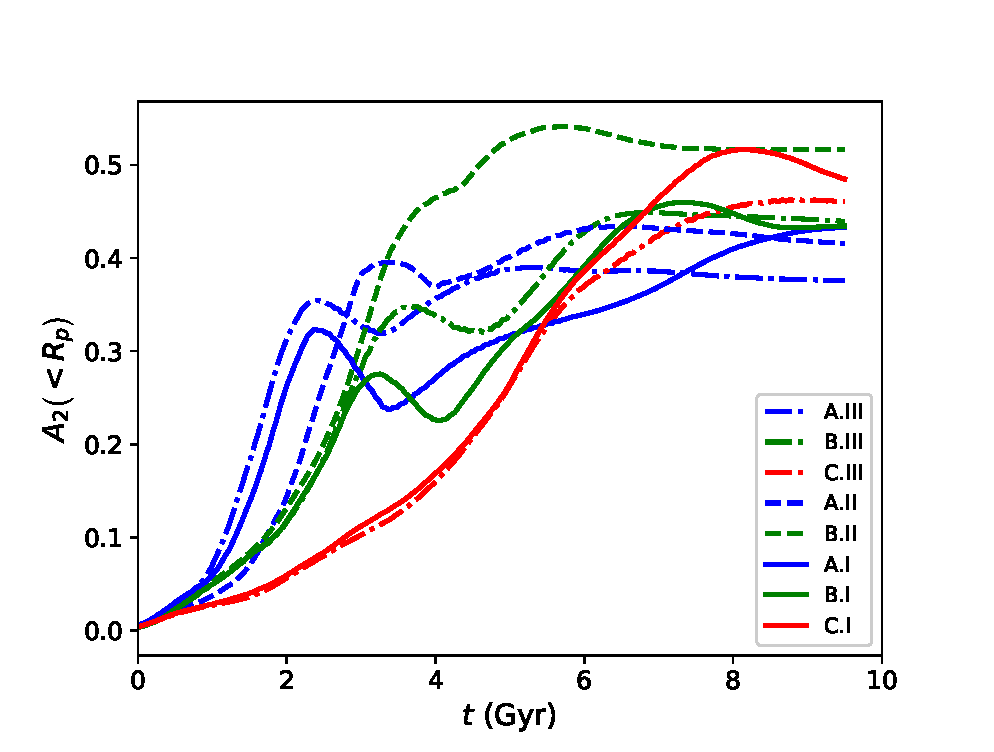
\includegraphics[width=0.9\textwidth]
{../figures/isolated_a2_vs_t_2rd_no_buckling_weighted.eps}
	\caption{Mean bar strength parameter inside the cylindrical
          radius $R_p$, $A_2(<R_p)$, as a function of time.  The
          figure is essentially the same as
          Fig.\,\ref{fig:isolated_a2_vs_t} though this time we include
          simulations A.III, B.III, and C.III where buckling is
          suppressed.} \label{fig:isolated_a2_vs_t_no_buckle}
\end{figure}


\begin{figure*}
	\centering
	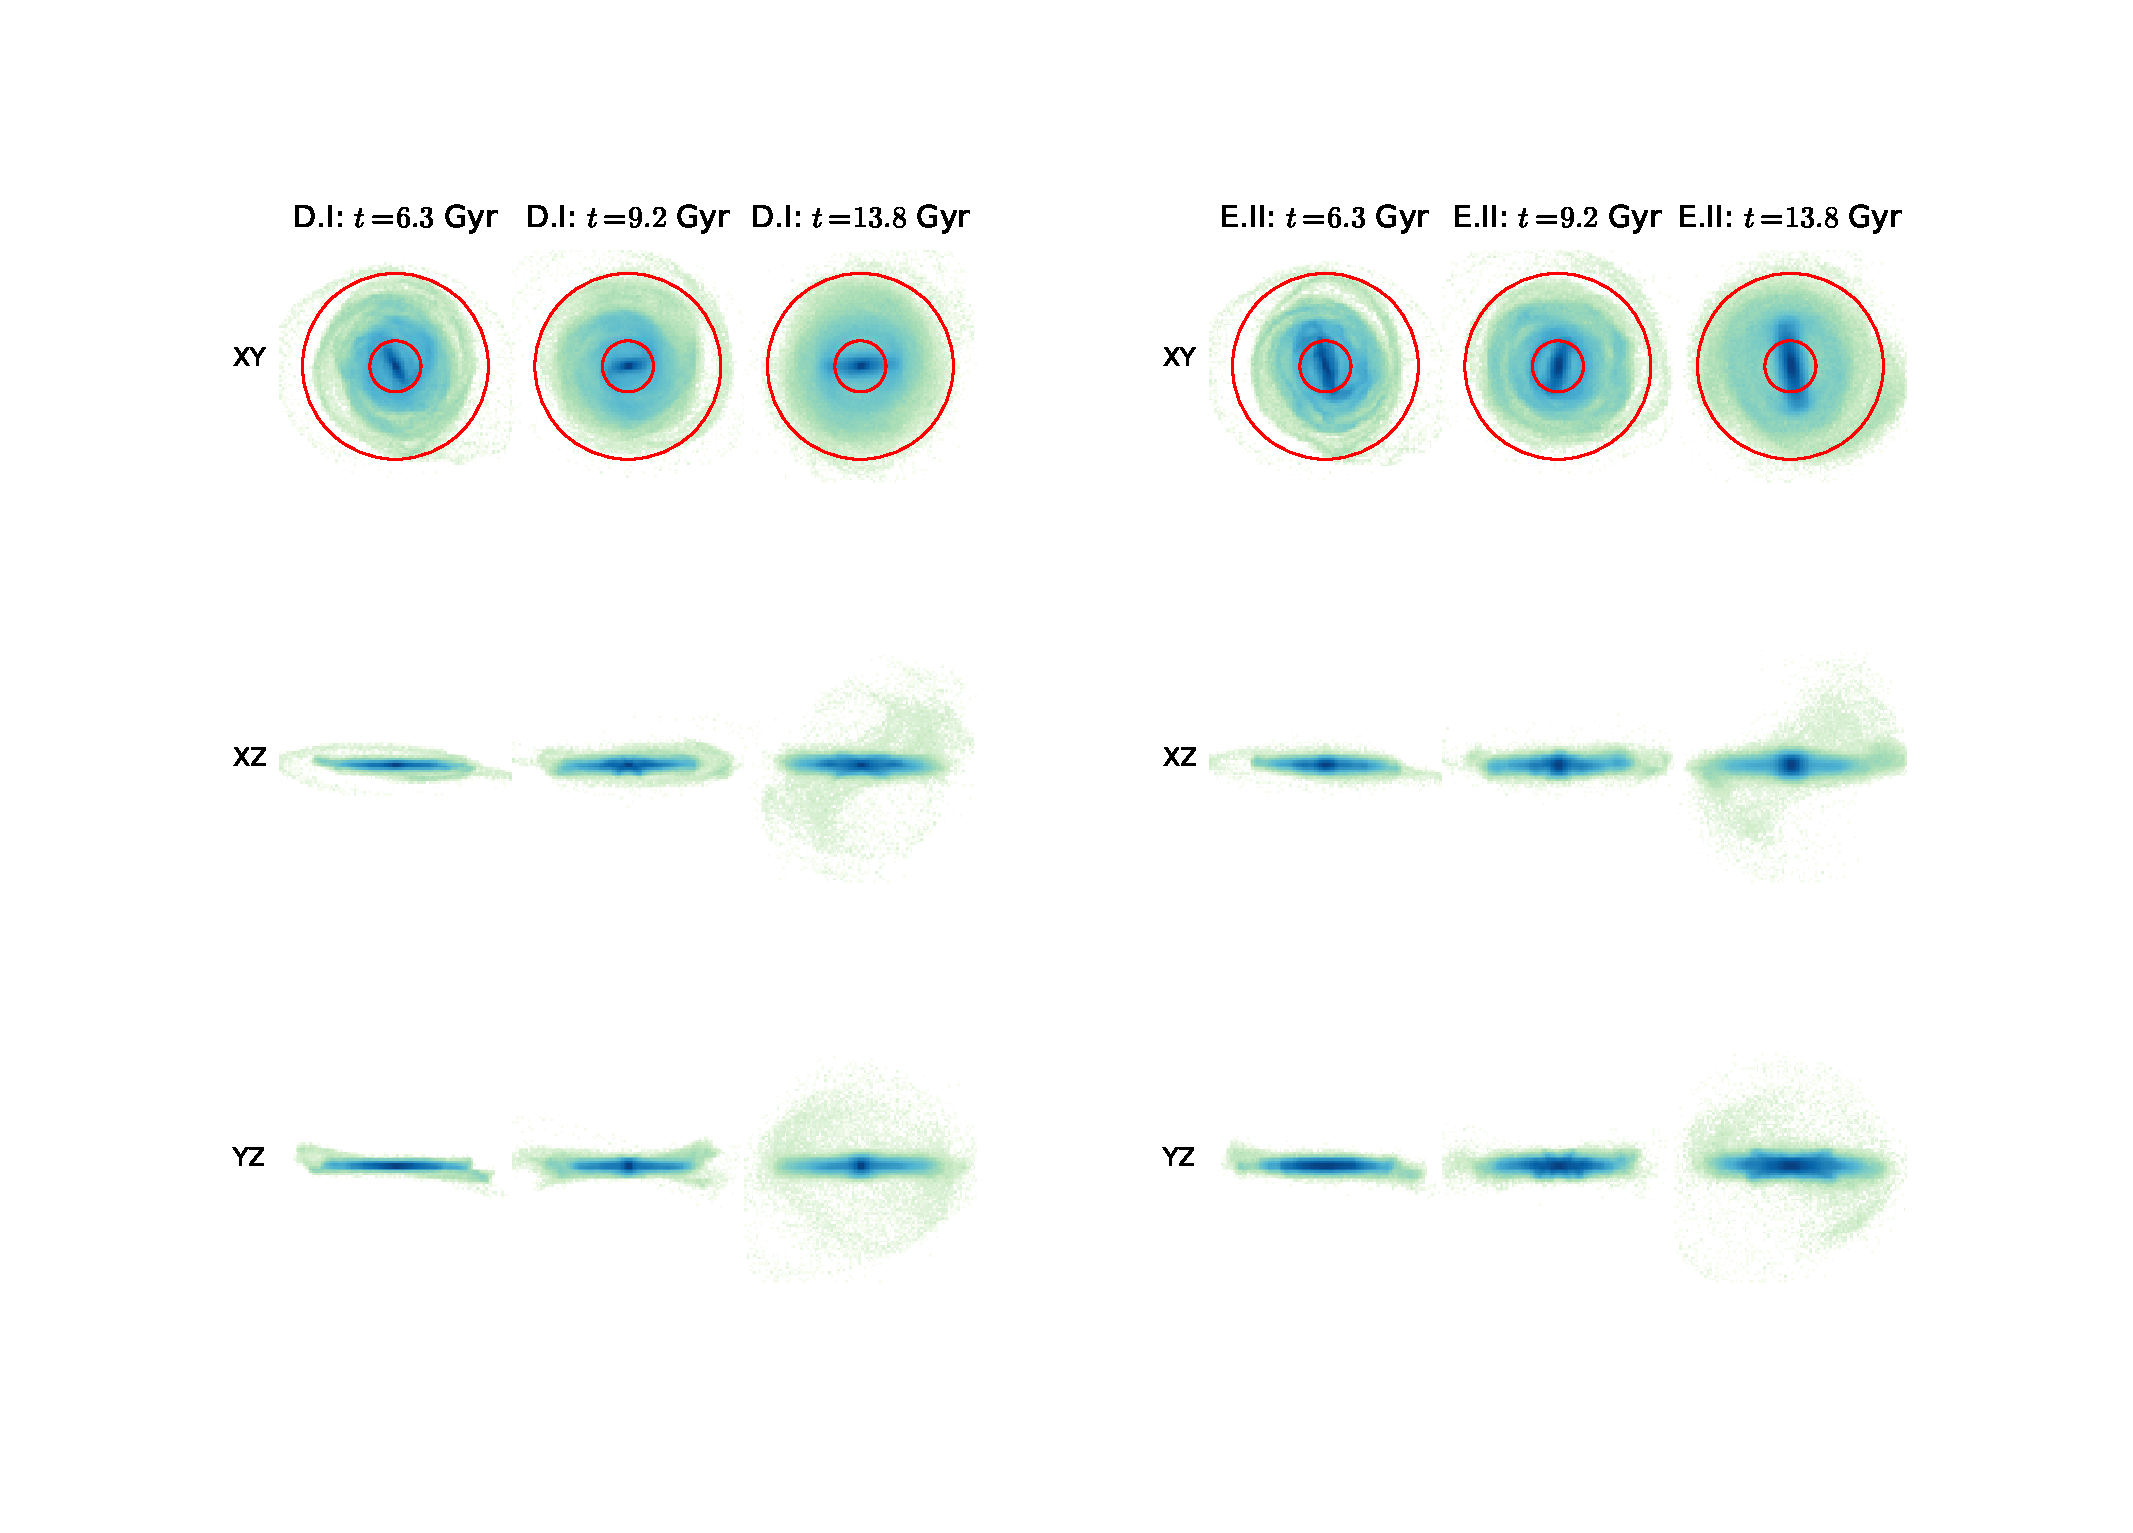
\includegraphics[width=\textwidth]{../figures/cosmo_three_by_threes.eps}
	\caption{Projections for the D.I (left three columns) and E.II
          (right three columns).  The three columns for each
          simulation correspond,from left to right, to $2.2\,{\rm
            Gyr}$, $5.9\,{\rm Gyr}$, and $13.7\,{\rm Gyr}$ after the
          Big Bang. The overlaid red circles have radii $R_p$ and 20
          $h^{-1} \,$kpc.} \label{fig:face_on_cosmo}
\end{figure*}

\begin{figure}
	\centering
	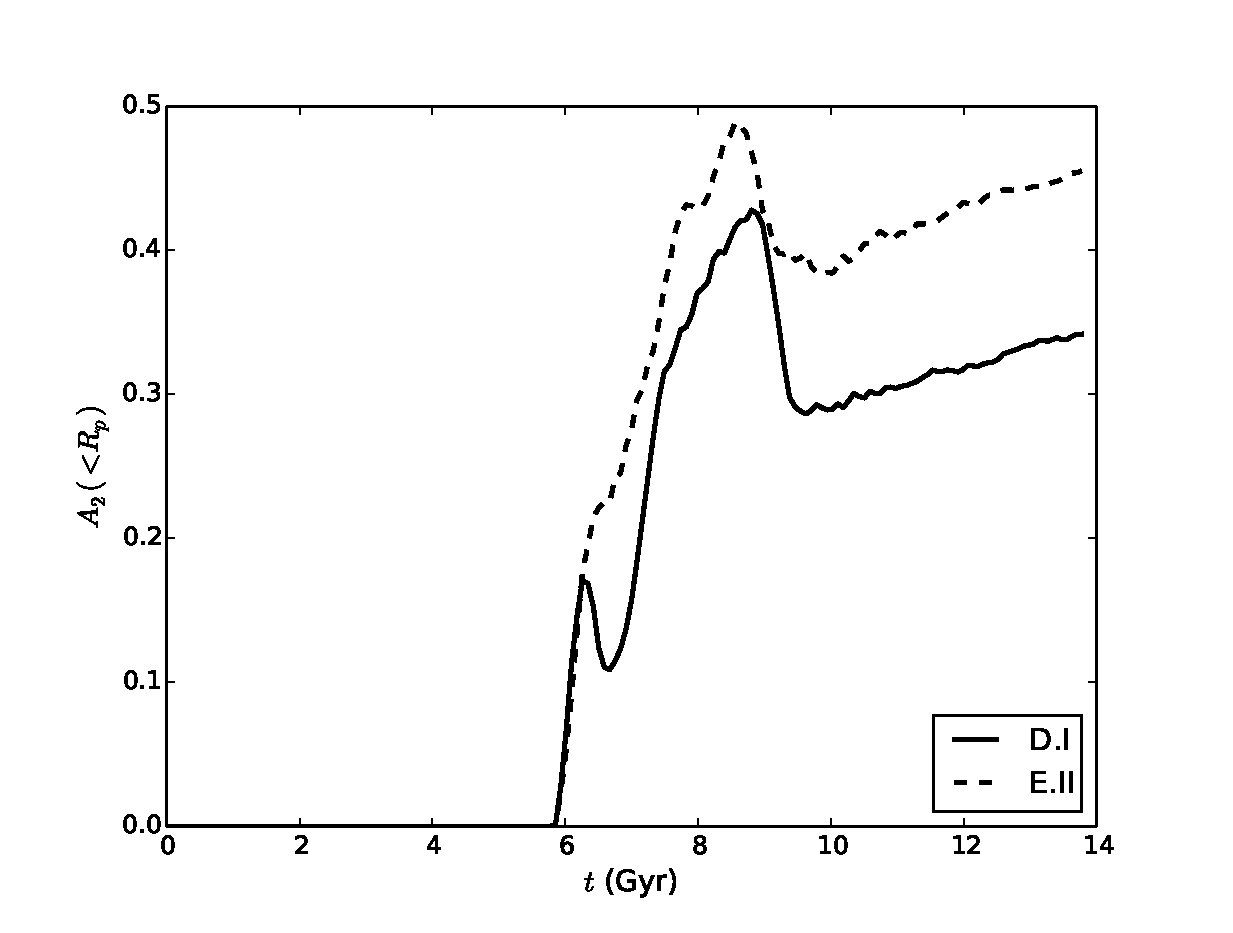
\includegraphics[width=0.9\textwidth]{../figures/cosmo_a2_vs_t_2rd_weighted.eps}
	\caption{$A_2(<R_p)$ as a function of the age of the Universe
          for simulations D.I (solid curve) and E.II (dashed
          curve). } \label{fig:cosmo_a2_vs_t}
\end{figure}


\begin{figure}
	\centering
	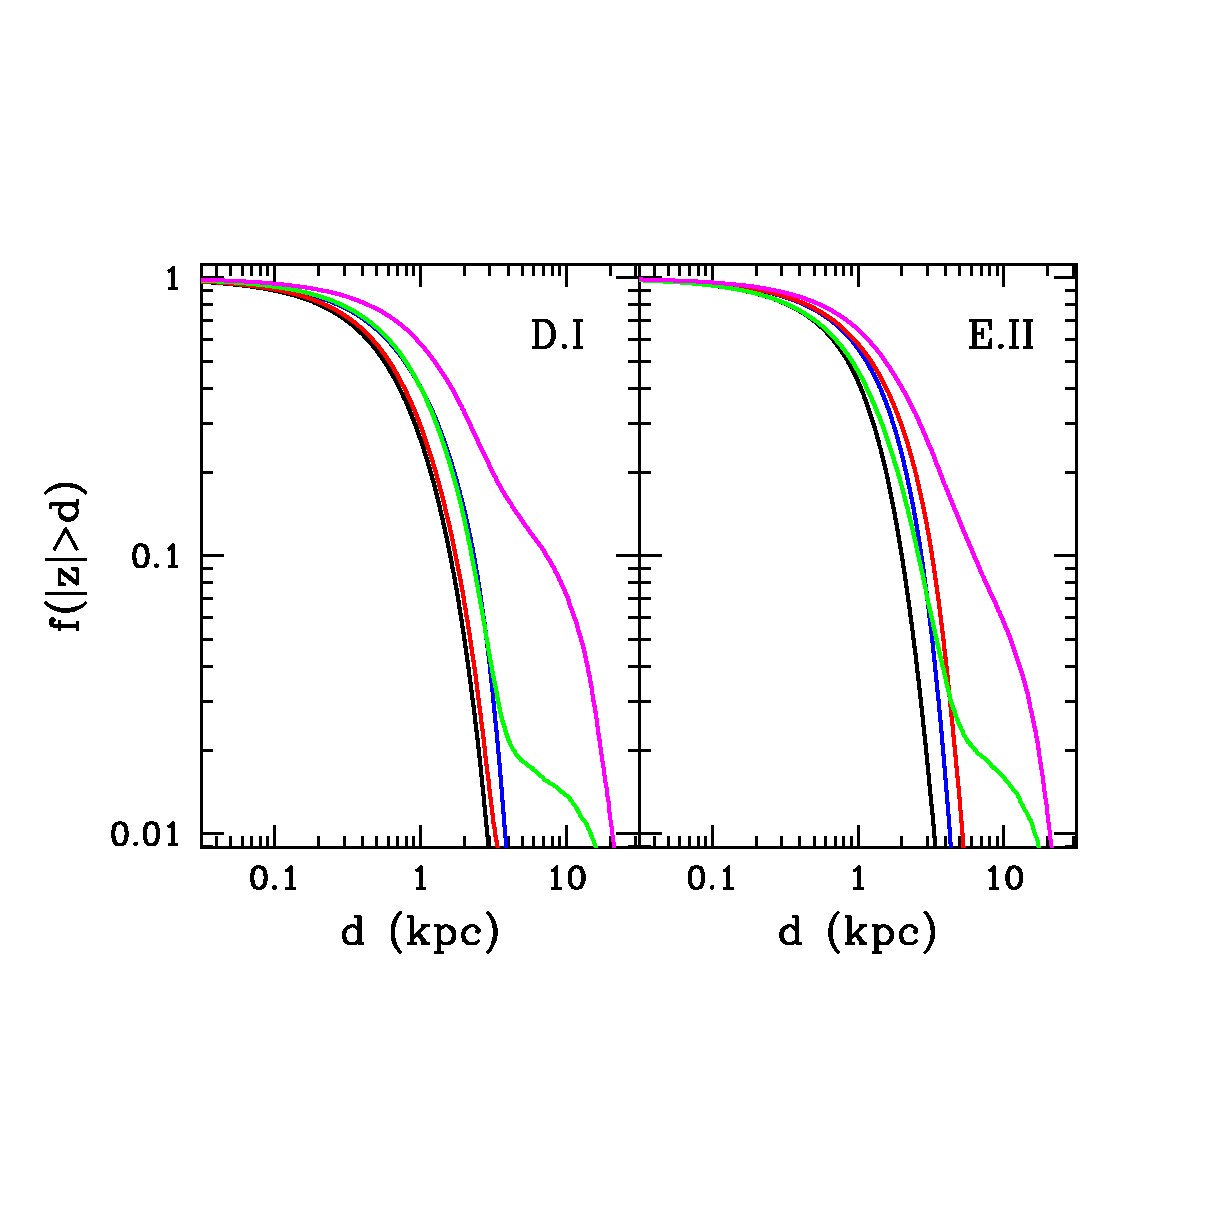
\includegraphics[width=0.9\textwidth]{../figures/kicked_up_disk.eps}
	\caption{Fraction of particles with distance from the midplane greater
than some distance $d$ as a function of $d$.  The difference colours correspond to
different bins in cylindrical radius $R$: $0<R<5\,{\rm kpc}$ --- black;
$5\,{\rm kpc} < R < 10\,{\rm kpc}$ --- blue;
$10\,{\rm kpc} < R < 15\,{\rm kpc}$ --- red;
$15\,{\rm kpc} < R < 20\,{\rm kpc}$ --- green;
$20\,{\rm kpc} < R\,{\rm kpc}$ --- magenta.}
 \label{fig:kicked_up_disc}
\end{figure}

\section{Cosmological Simulations} \label{sec:cosmo}

Disc galaxies simulated from axisymmetric, equilibrium initial
conditions, as was done in the previous section, form bars at rates
and with strengths that depend on their intrinsic scale height of the
disc and on the force resolution of the simulation. In this section,
we investigate the extent to which these results hold in a
cosmological environment.  In particular we follow the evolution of a
thin disc with moderate softening and a thick disc with high softening
that are embedded in identical cosmological haloes.

\subsection{Simulation Setup; Inserting Discs into Cosmological Haloes}

We model a stellar disc in a cosmological halo using the disc
insertion scheme described in \citet{Bauer2018a}.  This scheme, which
builds on the methods developed by
\citet{BerentzenShlosmanStellarDisks}, \citet{DeBuhrStellarDisks}, and
\citet{YurinSpringelStellarDisks} uses an iterative procedure to
initialize the disc.  The first step is to run a pure dark matter
simulation and identify a suitable halo.  The system is then rerun
from redshift $z_g$ to $z_l$, this time with a disc potential that
grows slowly in mass and radius.  Doing so allows the halo particles
to respond to the gravitational field of the would-be disc.  At $z_l$,
the rigid disc is replaced by an N-body system and the ``live'' disc-halo
system is evolved to the present epoch.

For our pure dark matter simulation, we implement the zoom-in
technique of \citet{KatzQuasarZoom} and \citet{NavarroWhiteZoom},
broadly following the recommendations of \cite{onorbe_etal_2014},
which allows us to achieve very high spatial and mass resolution for a
single halo while still accounting for the effects of large-scale
tidal fields.  We choose cosmological parameters based on the results
from Planck 2013 \citep{planck_2014} with $H_0=67.9\,{\rm
  km\,s}^{-1}\,{\rm kpc}^{-1}$, $\Omega_b = 0.0481$, $\Omega_0 =
0.306$, $\Omega_\Lambda = 0.694$, $\sigma_8 = 0.827$, and $n_s =
0.962$.  N-body initial conditions for the dark matter particles are
generated with the \textsc{music} code \citep{music}.  
We select a suitably-sized halo for a Milky Way-like galaxy, namely
one with a $z=0$ mass of $1.23\times 10^6\,h^{-1} M_\odot$
that comprises $10^6$.

During its growth phase from $z_g=3$ to $z_l=1$, the disc is treated
as a rigid body whose orientation and center-of-mass position evolve
according to the standard equations of rigid body dynamics.  At
$z_l$, we swap a live disc for the rigid one using the
\textsc{GalactICS} code
\citep{KGGalactICSReference,WPDGalactICSReference}, which generates a
three-integral DF disc in the best axisymmetric approximation to the
halo \citet{Bauer2018a}.

We run two simulations, D.I, which assumes a thin disc with a
softening length of $184\,{\rm pc}$ and E.II, which assumes a thick
disc with a softening length of $736\,{\rm pc}$.  The softening length
chosen for D.I is in accord with the criteria outlined in
\citet{power_et_al_2003}.  The simulations D.I and E.II roughly
correspond to A.I and B.II, respectively.  As well, E.II is similar to
the discs considered by \citet{DeBuhrStellarDisks},
\citet{YurinSpringelStellarDisks} and \citet{Bauer2018a}, whereas D.I
is more consistent with typical discs considered in isolated galaxy
suites like \citet{WPDGalactICSReference}.

\subsection{Results}

Results from our two cosmological simulations are displayed in
Figs.\,\ref{fig:face_on_cosmo} and \ref{fig:cosmo_a2_vs_t}.  The
former shows projections of the mass density at three epochs while the
latter gives $A_2(<R_p)$ as a function of time.  Evidently, the discs
in both cases roughly follow the same evolutionary sequence that was seen in
the isolated galaxy simulations: rapid growth of the bar strength
followed by a period where the bar strength decreases,
presumably due to buckling, and finally steady strengthening of the
bar.  The three epochs chosen in Fig.\,\ref{fig:face_on_cosmo}
correspond to the initial growth phase of the bar
($a=0.6,~t=6.3\,{\rm Gyr}$), an epoch after buckling
($a=0.7,~t = 9.2\,{\rm Gyr}$), and the present epoch at
$t=13.8\,{\rm Gyr}$.  Visually, the bar appears to be stronger and
longer in the E.II run than D.I one at each of these epochs but
perhaps most notably in the final one.  Indeed, the disc in E.II looks
very similar to those seen in the simulations of
\citet{DeBuhrStellarDisks}, \citet{YurinSpringelStellarDisks}, and
\citet{Bauer2018a}.  The fact that the bar in D.I is weaker than the
one in E.II is consistent with the results from our isolated galaxy
simulations that thicker discs produce stronger bars (See
Fig.\,\ref{fig:face_on_isolated}.

The most significant difference between bar formation in the
cosmological setting and bar formation in isolated galaxies concerns
the initial growth of the bar.  For isolated galaxies,
Fig.\,\ref{fig:isolated_a2_vs_t} clearly shows that the onset of bar
formation is delayed for thicker discs.  Conversely, in the
cosmological case, $A_2$ rapidly grows to a value of $\sim 0.17$
within the first few hundred Myr after the disc ``goes live''
regardless of the disc thickness.  At this point, the bar in the thin
disc model decreases in strength with $A_2$ dropping to $\sim 0.11$
before resuming its growth.  By contrast, the bar in the thick disc
model continues to grow monotonically.  As in the isolated galaxy
simulations, self-regulating processes such as buckling are more
efficient in the thin disc case and so $A_2$ in simulation D.I lags
behind that of E.II.  We note that in both cases, $A_2$ drops
significantly at around $t=7.5\,{\rm Gyr}$ and grows steadily
thereafter.

Our interpretation of these results is as follows: In isolation, where
discs start from axisymmetric initial conditions, the only source of
the $m=2$ perturbations that drive bar formation is shot noise from
the N-body distribution.  Evidently, making a disc thicker slows the
growth of these perturbations.  On the other hand, $m=2$ perturbations
abound in the cosmological environment where halos are clumpy and
triaxial.  The initial growth of the bar may, in fact, be relatively
insensitive to the thickness of the disc, once discs are placed in a
cosmological setting.  On the other hand, disc thickness does effect
the resilience of the bar to self-regulating processes, such that
buckling and therefore thick discs tend to have stronger bars.

Finally, we note that in both D.I and E.II, a significant number of
particles are found at high galactic latitudes.  These particles
represent stars ``kicked-up'' from the disc presumably by the
large-scale tidal fields of the halo and interactions between the disc
and halo substructure.  Kicked-up stars have been seen in cosmological
simulations by \citet{purcell2010}, \citet{mccarthy2012} and
\citet{tissera2013}.  Their existence was inferred in a combined
analysis of kinematic and photometric data for the Andromeda galaxy
\citep{dorman2013}.  Furthermore, the idea of kicked-up stars has been
invoked by \citep{pricewhelan2015} to explain the Triangulum-Andromeda
stellar clouds \citep{rochapinto2003, martin2014} and by
\citep{sheffield2018} to explain the Monoceros Ring \citep{yanny2000,
  newberg_2002} and associated A13 stellar overdensity
\citep{sharma2010}.

In Fig.\,\ref{fig:kicked_up_disc} we show the fraction of stars with
$|z|>d$ for different regions of the discs in our two cosmological
simulations.  The results are strikingly similar for the two
simulations as is already evident from a visual inspection of 
Fig.\,\ref{fig:face_on_cosmo}. The implication is that
the processes by which stellar orbits are
perturbed out of the disc plane are relatively insensitive to the
vertical structure of the disc.  We see that very few of the stars
with cylindrical radius $R<15\,{\rm kpc}$ and only $1-2\,\%$ of the
stars between $15$ and $20\,{\rm kpc}$ are kicked-up to distances
greater than $3\,{\rm kpc}$ though some stars from the $15-20\,{\rm
  kpc}$ region do end up with $|z|> 10\,{\rm kpc}$.  On the other
hand, $20\,\%$ of the stars from the region beyond $20\,{\rm kpc}$ end
up with $|z|> 3\,{\rm kpc}$ from the midplane and $10\,%$ end up $|z|>
10\,{\rm kpc}$.  Of course, the actual number of stars is certainly
larger since a fraction of the kicked-up stars will be passing through
the disc with large vertical velocities.

\section{Conclusions}\label{sec:conclusions}

The seminal work of \citet{PeeblesOstriker1973} introduced the notion
that disc dynamics provides a powerful constraint on the structure of
discs and the halos in which they reside.  In short, discs that are
dynamically cold and that account for a substantial fraction of the
gravitational force that keeps their stars on nearly circular orbits
are unstable to the formation of strong bars and spiral structure.
The existence of galaxies with weak bars or no bars at all tells us
that at least some discs are relatively low in mass (i.e., submaximal)
and/or dynamically warm.

The theoretical analysis presented in Section 2 showed with a few
simple assumptions (e.g., exponential surface density profile) one can
derive a relation among the structural parameters of a disc in
approximate equilibrium and thus a constraint on initial conditions
that one might choose for simulations.  For example, if one fixes
$h_d/R_d$ and $\sigma_R/\sigma_z$, as was done in
\citet{YurinSpringelStellarDisks}, then there is an approximately
one-to-one relationship between $Q$ and $X$.  Likewise, fixing $Q$ and
$X$ implies a relationship between $h_d/R_d$ and $\sigma_R/\sigma_z$.
These results have important implications for applying disc dynamics
as a constraint on models of galaxy formation.  In particular,
inconsistencies between bar demographics in a galaxy formation model
and in observational surveys may reflect differences in the scale
height and vertical velocity dispersion of model and real galaxies.

One lesson from our work and the work of others is that the relation
between structural parameters of galaxies and bar strength and length
is often rather complicated.  This observation is no doubt due, at
least in part, to the self-regulating nature of bar formation.  When
bars develop rapidly, they tend to buckle, which leads to weaker and
shorter bars \citep{VP2004}.  Thick discs appear to be more resilient
to buckling, which may explain why bars in these models often end up
stronger and longer than bars in thin-disc models \citep{Klypin2009}.
For similar reasons, gravitational softening can affect the
development and ultimate strength of bars.

In simulations of isolated galaxies from ``pristine'' equilibrium
initial conditions, bar formation is seeded by the shot noise of the
N-body distribution.  On the other hand, bars in a cosmological
environment are subjected to large perturbations including the $m=2$
ones that drive bar formation.  Thus, the fact that bar formation is
delayed in thick disc models of isolated galaxies may be purely
academic --- bar formation in the cosmological environment will be
initiated by a variety of stochastic effects regardless of the
thickness of the disc.  On the other hand, the resilience of thick
disks to buckling {\it is} relevant in the cosmological setting and
may explain why thick disks tend to form strong bars.  The upshot is 
that a proper understanding the distribution of bars in cosmological models
must go hand-in-hand with a proper understanding of the vertical 
structure of discs.

Clearly, a more exhaustive exploration of the model parameter space is
in order.  One might, for example, include galaxy scaling relations to
further constrain the space of models.  In addition, it would be of
interest to insert different discs (and for that matter, nearly
identical ones) into different halos in order to explore the
random nature of disc-halo interactions.  Ultimately, improvements
in observations together with a more complete survey of models via
simulations should allow us to fully exploit bars in discs as a means
of testing and constraining theories of structure formation.

\section*{Acknowledgements}
{LMW and JB are supported by a Discovery Grant with the Natural
  Sciences and Engineering Research Council of Canada. JSB
  acknowledges the assistance of Matthew Chequers and Keir Darling in
  understanding the \textsc{AGAMA} program interface.}

% The best way to enter references is to use BibTeX:

\bibliographystyle{apalike}
\bibliography{bibliography_paper_ii.bib} % if your bibtex file is called example.bib

\newcommand{\kpch}{\ensuremath{h^{-1} \, \text{kpc}}}
\newcommand{\kpc}{\ensuremath{\text{kpc}}}
\newcommand{\solarmh}{\ensuremath{h^{-1} \, M_\odot}}
\newcommand{\solarm}{M_\odot}
\chapter{Forming Vertical Structure in $\Lambda$CDM Discs}\label{ch:paper_iii}
\textbf{This chapter contains a draft of a paper in preparation to be submitted to Monthly Notices of the Royal Astronomical Society. The working title for the paper is ``Vertical Structure and Kicked-Up Stars in $\Lambda$CDM Galaxies". }

\newpage
\section{Abstract}

We perform numerical experiments where stellar discs are inserted into
dark matter halos in a $\Lambda$CDM simulation after which the
fully-live disc-halo systems are evolved until the present epoch. {Prior it its insertion, a disc is treated as a growing, rigid potential whose position and orientation are determined from rigid-body dynamics. When the disc goes live, the disc-halo system is in approximate equilibrium.} The
discs develop structures such as bars, warps, and bending waves.  Not
surprisingly, we find that when we insert the disc at a redshift
$z=1$, it develops more structure and exhibits more clearly signs of
disequilibrium then when it is inserted later.  We identify
populations of stars kicked out of the disc to high latitudes that are
qualitatively similar what is observed in the Milky Way. {An in-depth attempt is made to disentangle the effects of bar buckling, tidal fields due to 
the generally triaxial halo and from distant subhalos, and the
passage of subhaloes through the inner disc. }While our
results are consistent with the hypothesis the the kicked-out-disc was
produced by a very massive satellite galaxy, we also find that they
can arise from the interaction of the disc with its halo. We conclude
that in the Milky Way a wide variety of cosmological environments are
able to explain disc structures like Monoceros, A13, and TriAnd.


%%%%%%%%%%%%%%%%%%%%%%%%%%%%%%%%%%%%%%%%%%%%%%%%%%

%%%%%%%%%%%%%%%%%%%% REFERENCES %%%%%%%%%%%%%%%%%%

% The best way to enter references is to use BibTeX:
\section{Introduction} \label{sec:introduction}

The \textsc{Hi} discs of late-type galaxies, when observed edge-on,
often exhibit pronounced warps (see, for example,
\citet{sancisi_1976,bosma_1991, garcia-ruiz_2002} and reviews by
\citet{binney_1992} and \citet{Sellwood2013}). Indeed, the \textsc{Hi}
warp in the Milky Way has been known since the work of
\citet{oort_1958}. There is also evidence for a stellar warp in the
Milky Way, which roughly traces that of the \textsc{Hi} disc
\citep{cox_1996, reyle_2009}.

The prevalence of warps suggests that a typical stellar disc
experiences perturbations normal to its midplane. Recent surveys,
particularly of the stellar content in the Galaxy, have revealed other
manifestations of vertical perturbations. For example, surveys such as
the Sloan Extension for Galactic Understanding and Exploration (SEGUE)
and Gaia Data Release 2 (GDR2) have uncovered an asymmetry with
respect to the Galactic midplane in stellar number counts in the
vicinity of the Sun \citep{widrow_2012_sdss, yanny_gardner_2013,
  bennet_2019_gaia}. In addition, bulk motions of stars normal to the
midplane have been found in data from SEGUE, the Radial Velocity
Experiment (RAVE), the LAMOST survey, and GDR2
\citep{widrow_2012_sdss, williams_2013_rave, carlin_2013_lamost,
  pearl_2017, carrillo_2018_rave, gaia_collab}. Furthermore, a
corrugation in stellar number counts with a wavelength of $\sim
5\,{\rm kpc}$ and an amplitude of $\sim 100\,{\rm pc}$ has been
detected between $10$ and $15$ kpc in Galactocentric radii
\citep{xu_2015}. Corrugations in the velocity field of gas discs
in external galaxies have also been observed \citep[for
  example]{matthews_2008,sanchez_2015}.

In addition to waves and corrugations, several stream-like stellar
structures in the Milky Way may have originated within the
disc. In the past, these structures were thought to comprise stars
tidally stripped from disrupted dwarf galaxies or globular
clusters. Recently, the idea that some of the streams are actually
stars 'kicked out' of the disc has gained traction. One example is the
Monoceros ring \citep{newberg_2002, yanny_2003}, also called the
Galactic Anticentre Stellar Structure (GASS) \citep{crane_2003,
  rocha-pinto_2003}, which is located at low latitudes towards the
Galactic anti-centre at a Galactocentric distance of about
$18\,\,\kpc$. The coincidence in position and velocity of GASS and
disc stars suggests that a disc origin may be a more likely explanation than tidal stripping \citep{deason_2018,
  monoceros_disk_origin}. Similar structures have been found in the
outer disc, most notably the Triangulum-Andromeda clouds (TriAnd)
\citep{triand_discovery} and A13 \citep{a13_discovery}. There is also
evidence for kicked-out stars in M31 \citep{richardson_2008_m31,
  dorman_2013_m31, bernard_2015_m31} and M33
\citep{mcconnachie_2006_m33, mcconnachie_2010_m33}. (For a review of
the kicked-out-disc hypothesis, see \citet{johnston_kud_review}.)

There is now a concerted effort to explain vertical disequilibria in
Milky Way-like galaxies. Much of this effort has focused on the
hypothesis that a single massive subhalo, such as the Sagittarius
dwarf spheroidal galaxy (Sgr dSph) \citep{ibata_discovery}, is
responsible for much of the vertical structure in the Milky
Way. Simulations of a single satellite encounter with an isolated
galaxy have been used to study this hypothesis \citep[for
  example]{purcell2011,gomez_2013,widrow_2014,feldmann_2015, dlv_2015,
  donghia_2016, laporte_2016, laporte_2018, laporte_2018_b}. While
many of the observed features are easily reproduced in the
simulations, it appears that a very massive ($10^{11}\,\solarm$) Sgr
dSph-like satellite is required to explain the extraplanar streams in
the outer disc \citep{laporte_2018_b}.

The single-satellite encounter is a rather idealized scenario;
disc-environment interactions in real galaxies will, of course, be
more complicated. In particular, discs may be continually perturbed by
any number of satellites or dark matter subhaloes whose orbits take
them into the disc region of the galaxy. Early steps toward a more
realistic model were taken by \citet{font_2001} and
\citet{gauthier_2006} who allowed for a system of subhalos. In
particular, \citet{gauthier_2006} simulated an M31-like disc in a dark
halo where roughly 10\% of the smooth halo mass was replace by dark
subhalos with a mass spectrum motivated by cosmological $\Lambda$CDM
simulations. They found that one or more of the subhalos triggered the
formation of a bar. Further analyses of this simulation and a similar
one by \citet{chequers_2018} found that the system of subhalos could
excite a plethora of vertical structure. However, these simulations
failed to create the streams of disc stars described above.

When a satellite passes through the plane of disc, it interacts with
the disc through a process akin to dynamical friction. Essentially,
disc stars fall in behind the satellite, disrupting and ultimately
heating the disc \citep{sellwood_1998}. On the other hand a distant
but very massive satellite can excite bending modes via differential
acceleration. In the simple example of a satellite falling toward the
disc along its spin axis, the acceleration of the disc toward the
satellite decreases with radius. Thus, as the satellite passes
through the centre of the disc, it will set up axisymmetric bending
modes as seen in \citet{sellwood_1996}.

Finally, we note that dark halos in $\Lambda$CDM cosmologies are
thought to be aspherical and will therefore exert torques on the disc
that can cause it to bend and warp. The effect is due to a
misalignment of the disc symmetry axis with any of the approximate
symmetry axes of the halo. For example, \citet{hu_2016} embed discs
in triaxial haloes. In their appendix, strong warps can be seen in
discs which are substantially misaligned from their
haloes. \citet{gomez_2017} found that vertical structure was
ubiquitous in their hydrodynamical cosmological simulations, some of
which did not have discs in a stable orientation to their host halo.

In this paper, we study the vertical structure that develops in discs
embedded in realistic $\Lambda$CDM haloes. We use a disc insertion
scheme to set up initial conditions where a stellar disc is in
approximate equilibrium with a cosmological halo
\citep{berentzen_2006, debuhr_2012, ys_2015, bauer2018a, hu_2018}. Our
scheme affords us more control over the structural properties of the
disc than would be possible in fully self-consistent hydrodynamical
simulations and was successfully used to study bar formation in a
cosmological context in \citet{bauer2018b}. In fact, bar buckling is
another mechanism for exciting vertical structure in stellar discs
\citep{bar_buckling_echo}, a point we return to later in this paper.

Our paper is organized as follows: In \S\ref{sec:overview} we present
two toy models that serve to illustrate the mechanisms by which
satellites can excite bending modes in a stellar disc. An overview of
the cosmological simulations is given in \S\ref{sec:description} while
the time evolution and key structural features of the discs in these
simulations are discussed in \S \ref{sec:evolution}. In \S\ref{sec:kud}
we examine how stars are kicked out of discs.  We relate our key
results to other studies in \S\ref{sec:discussion} and present a
summary and some concluding remarks in \S\ref{sec:conclusion}.

\begin{figure}
	\centering
	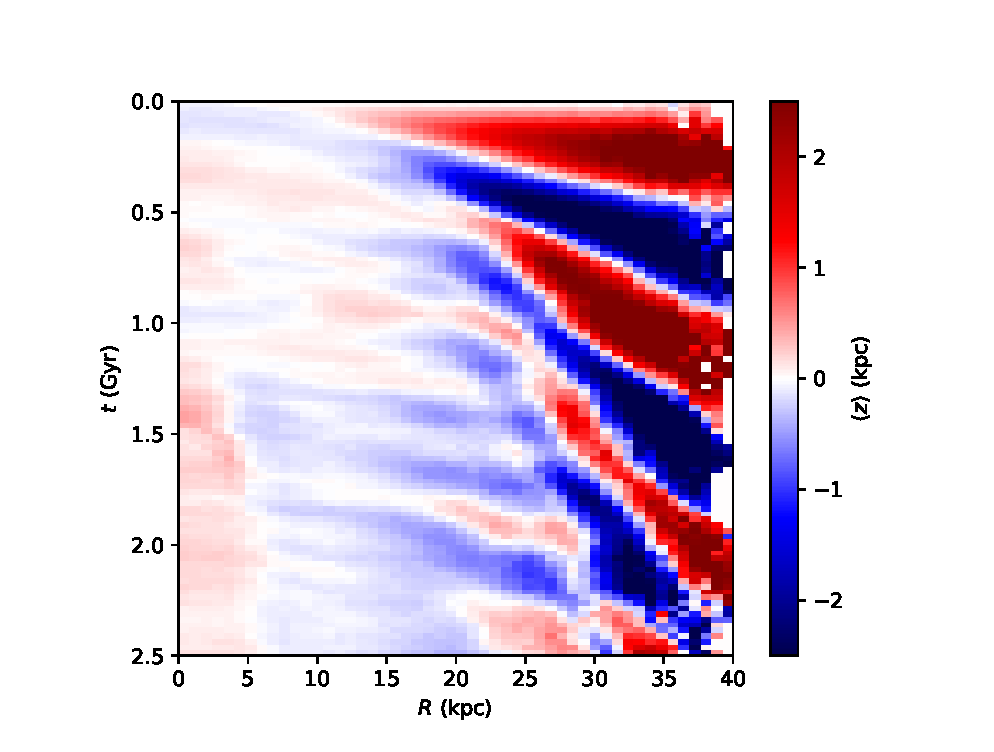
\includegraphics[width=0.85\textwidth]{../figures/isolated_z_0_r_a.eps}
	\caption{Mean vertical displacement, $\langle z \rangle$, of the disc for the
          toy model described in \S\ref{ssec:toy_model_1} as a
          function of $R$ and $t$.} \label{fig:toy_model_1_mean_height}
\end{figure}

\begin{figure}
	\centering
	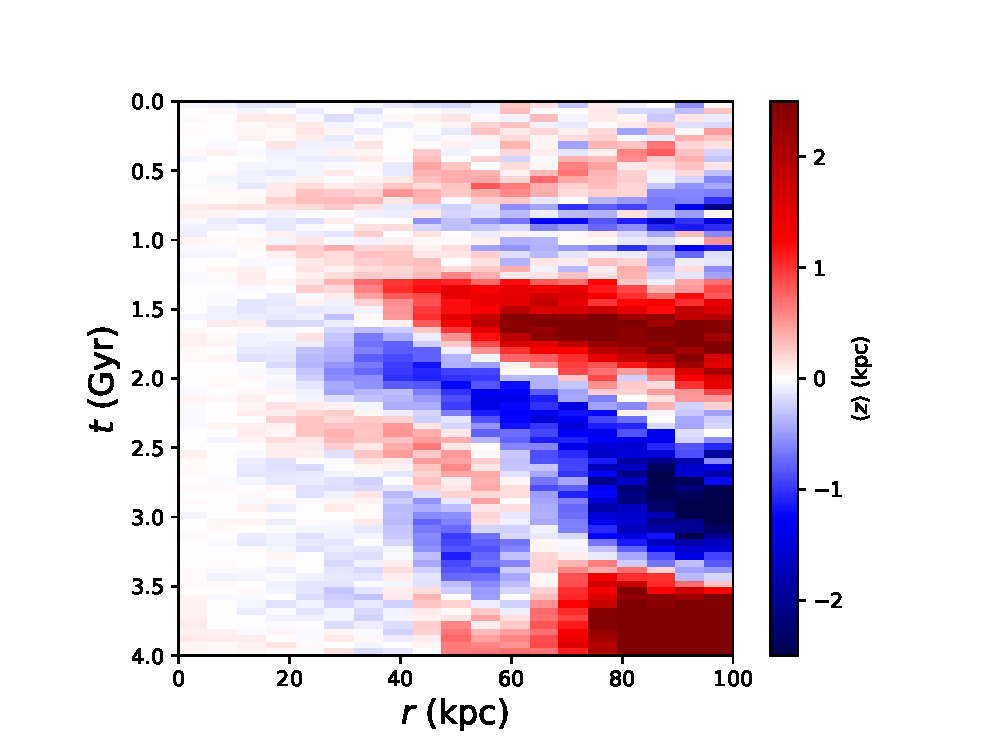
\includegraphics[width=0.85\textwidth]{../figures/isolated_z_0_r_a_halo.eps}
	\caption{Mean vertical displacement of the halo in the toy model described in
          \S\ref{ssec:toy_model_1} as a function of spherical radius $r$ and $t$.} 
        \label{fig:toy_model_1_mean_height_halo}
\end{figure}

\section{Single satellite simulations} \label{sec:overview}

In this section, we illustrate some of the factors driving vertical
structure in stellar discs through two toy models where a disc
interacts with a single subhalo.

\subsection{Axisymmetric subhalo encounter} 
\label{ssec:toy_model_1}

In our first experiment, the subhalo is initially at rest and
positioned $100\,{\rm kpc}$ from the centre of the disc along its
symmetry axis. We generate the initial conditions for the disc, halo,
and subhalo using the \textsc{GalactICS} code
\citep{KGGalactICSReference,WPDGalactICSReference}. The disc has an
exponential surface density with scale length $R_d=3.7\,\kpc$ and mass
$M_d=4\times10^{10} \,\solarm$. The halo has an NFW density profile
\citep{navarro_1997}, with scale length $R_h=33.2\,\kpc$, virial mass
$M_h=1.1\times10^{12}$, and concentration $c=6.7$. We use $10^6$ halo
particles and $3.5 \times 10^{6}$ disc particles. The subhalo is also
assumed to have an NFW profile with scale length $R_h=1.70\,\kpc$,
virial mass $M_h=2.7\times10^{10}$, and concentration $c=38.1$. The
choice of parameters for the disc, halo, and subhalo are motivated by
examples from our suite of cosmological simulations. The simulation is
performed using \textsc{Gadget-3}, a privately released version of the
popular \textsc{Gadget-2} code \citep{GadgetCodePaper}.

In Fig. \ref{fig:toy_model_1_mean_height} we show the azimuthally
averaged vertical displacement, $\langle z\rangle(R,\,t)$. The displacement
is relative to the disc midplane, defined by the mean $z$ of all the
particles. {
This quantifies axisymmetric vertical perturbations, that is, $m=0$
vertical perturbations where $m$ is the azimuthal mode number.  More generally, for a quantity $\Theta$, we define the $m$-fold symmetric $\Theta_m$,}
\begin{eqnarray}
\Theta_{m} &=&\frac{1}{M_S} \int_S \text{d}^3 \textbf{r} \text{d}^3\textbf{v} f(\textbf{r}, \textbf{v}) \Theta(\textbf{r} , \textbf{v})e^{i m \phi_j}\\
&\approx& \frac{1}{M_S} \sum_{j \in S} m_j \Theta(\textbf{r}_j, \textbf{v}_j)e^{im \phi_j} \label{eq:z_statistic}
\end{eqnarray}
{where $M_S$ is the mass in a region $S$, $f(\textbf{r},\textbf{v})$ is the phase space distribution function, $\phi_j$ is the azimuthal angle of the $j$-th particle in $S$, and $m_j$ is the mass of the $j$-th particle in $S$. 
}

At first the disc is relatively unperturbed; the subhalo is
so far away that it exerts an approximately uniform acceleration
across the disc. Only in the very outer disc do we see slight disc
flapping, that is, a lagging of the outer disc relative to the inner
one. The lag is more pronounce as the subhalo makes its first
pericentric passage. After the subhalo has passed through the disc, at
about $1\,{\rm Gyr}$, the pattern reverses as the center of the disc
is pulled back down. The resulting lag of the outer disc then shows up
as a positive signal. The disc develops a corrugation pattern as seen
in the alternating red and blue bands (positive and negative $\langle
z\rangle$). These bending waves propagate outward (bands stretch down
and to the right in the figure.) Over time, the wavelength decreases
as does the speed of propagation. Note that the strong ($> 1\,{\rm
  kpc}$) flapping of the disc beyond $20\,{\rm kpc}$ persists for many
dynamical times (see, also \citet{sellwood_1996}) and weaker
corrugation patters are seen further in.

Qualitatively similar behaviour is seen in the halo. In
Fig. \ref{fig:toy_model_1_mean_height_halo} we show $\langle
z\rangle$, this time averaged in spherical shells in the halo. At
early times, the halo is dragged along with the subhalo. Eventually,
we get a sloshing back and forth of the halo.

\begin{figure}
	\centering
        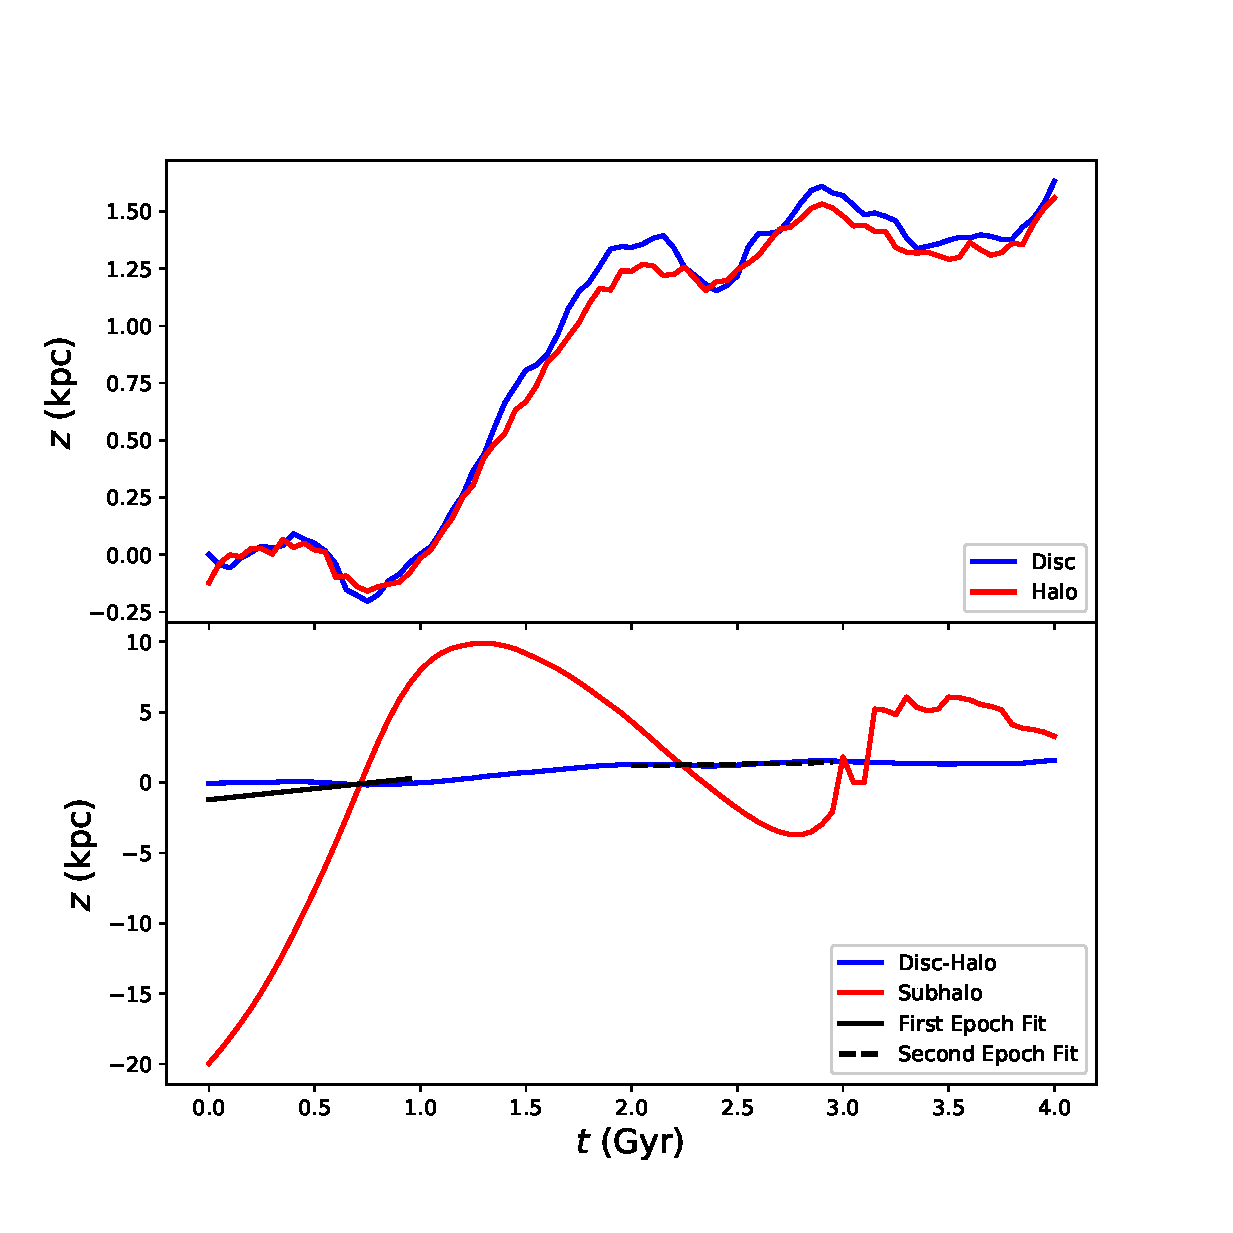
\includegraphics[width=0.85\textwidth]{../figures/isolated_orbits_two_fits_two_panel.eps}
	\caption{Top panel: Orbit of the disc (blue) and inner halo
          (red) in the toy model described in
          \S\ref{ssec:toy_model_2}. Only the $z$-components of the
          disc and halo position vectors are shown. Bottom panel:
          Orbits of the disc and inner halo (blue) and subhalo
          density peak (red).  The black lines show the fits for the
          two epoch as described in the
          text.} \label{fig:toy_model_2_orbits}
\end{figure}

\subsection{Off-axis subhalo encounter} \label{ssec:toy_model_2}
\begin{figure}
	\centering
	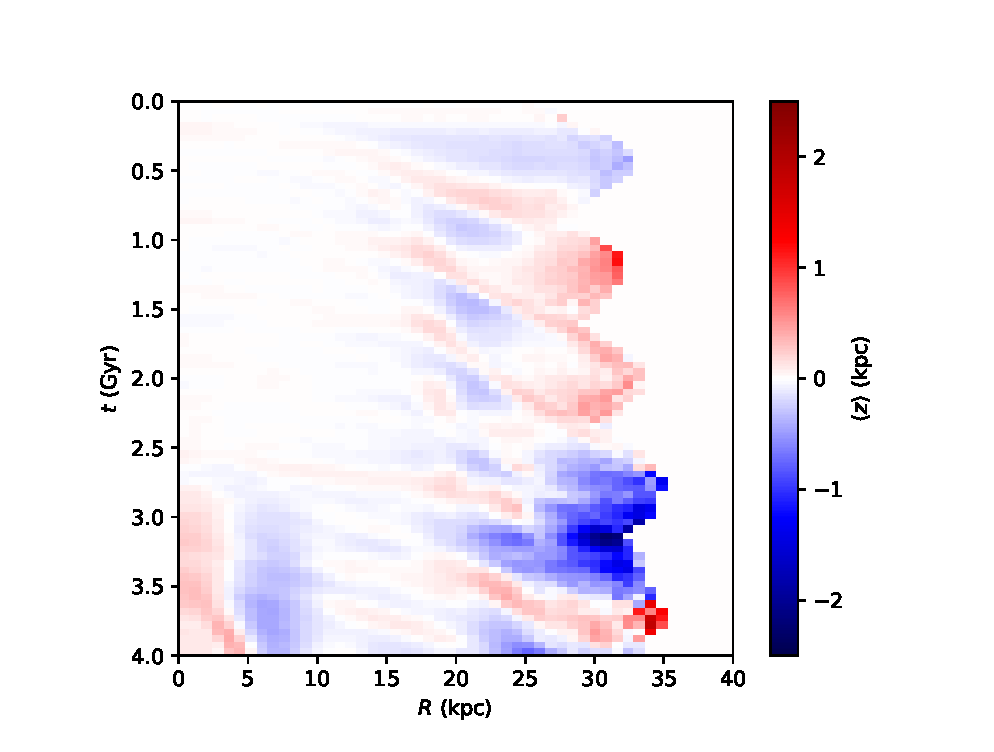
\includegraphics[width=0.85\textwidth]{../figures/b_late_light_subhalo_z_0_r_a.eps}
	\caption{Mean height, $\langle z \rangle$, of the disc for the
          toy model described in \S\ref{ssec:toy_model_2} as a
          function of $R$ and
          $t$.} \label{fig:toy_model_2_mean_height}
\end{figure}

In our second experiment, the satellite is again initialized at rest
$100\,{\rm kpc}$ from the centre of the disc, but this time at an
angle of just $12^\circ$ from the disc plane. The choice of orbit is
motivated by a satellite in one of our cosmological simulations. The
parameters for the disc, halo, and subhalo are the same as in
\S\ref{ssec:toy_model_1}.

In the upper panel of Fig. \ref{fig:toy_model_2_orbits} we plot the
$z$ coordinates of the position vector ${\bf r}_d$ of the disc and
${\bf r}_h$, the position vector of the peak halo density.  Evidently,
the halo density peak and centre of the disc closely track one
another. We next define a common position vector for the disc and
inner halo:
\begin{equation}
{\bf r}_{dh} = \frac{M_d {\bf r}_d + M_{h,20} {\bf r}_{h,20}}
{M_d + M_{h,20}}
\end{equation}
\noindent where we have arbitrarily used $20\,{\rm kpc}$ to define the
inner halo. Given the closeness of ${\bf r}_d$ and ${\bf r}_h$, the
choice of this definition shouldn't effect the results that follow.

Our working hypothesis is that during periods between perigalactic passages,
the subhalo and the combination of the disc and inner halo can be
treated as a two-body system. That is, ${\bf r}_{dh}$ and ${\bf
  r}_{sh}$, where the latter is the position vector for the peak of
the subhalo, satisfy the equation
\begin{equation}
\frac{M_{dh}\textbf{r}_{dh} + M_{sh} \textbf{r}_{sh}}{M_{dh} +
  M_{sh}} = \textbf{r}_{c,0} + \textbf{v}_{c,0} t
\end{equation}
where $M_{dh}$ and $M_{sh}$ are the effective disc-halo and subhalo masses.

To test our hypothesis, we maximize the likelihood function
\begin{equation}
\ln \mathcal{L} = -\frac{\chi^2}{2\sigma_d^2} - N\ln\sigma_d / \kpc
\end{equation}
over the parameters ${\bf r}_{c,0}$, ${\bf v}_{c,0}$, $M_{dh}$,
and $M_{sh}$. Here, $N$ is the number of snapshots, {$\sigma_d$ is the RMS difference between the model and the data, }and
\begin{equation}
\chi^2 = \left\vert
\frac{M_{dh}\textbf{r}_{dh} + M_{sh} \textbf{r}_{sh}}{M_{dh} + M_{sh}}
- (\textbf{r}_{c,0} + \textbf{v}_{c,0} t )\right\vert^2~.
\end{equation}
Maximization is done in two $1 \, {\rm Gyr}$  epochs centered on $0.5\,{\rm
  Gyr}$ and $2\,{\rm Gyr}$, respectively. These windows are chosen to
avoid the pericentric passages at $0.85\,{\rm Gyr}$ and $3\,{\rm
  Gyr}$, when the subhalo is losing the most mass when the system will
be poorly described by a two-body model. The center-of-mass motion
lines, $\textbf{r}_{c,0} + \textbf{v}_{c,0} t$ for the two epochs are
shown in Fig. \ref{fig:toy_model_2_orbits}. The inferred effective
mass ratios $M_{sh}:M_{dh}$ are 16:1 and 85:1, respectively.  Thus,
the effective mass of the subhalo has been reduced by a factor of
$\sim 5$, presumably due to tidal stripping. We also find that
$\sigma_d= 190\,{\rm pc}$ and $290\,{\rm pc}$ for the two epochs.  The
fact that the values for $\sigma_d$ are as small as they are supports
our hypothesis of a two-body model for the disc-halo/subhalo system.

In Fig. \ref{fig:toy_model_2_mean_height} we plot the mean height
across the disc as a function of radius and time. The general
corrugation pattern is similar to the one seen in our first experiment
though the amplitude is smaller. The difference in amplitude is no doubt
due to the fact that we are averaging over azimuth in an experiment
that lacks azimuthal symmetry.

\section{Simulations} \label{sec:description}

In this section, we summarize our cosmological simulations beginning
with a brief description of our disc insertion scheme.

\begin{figure}
	\centering
	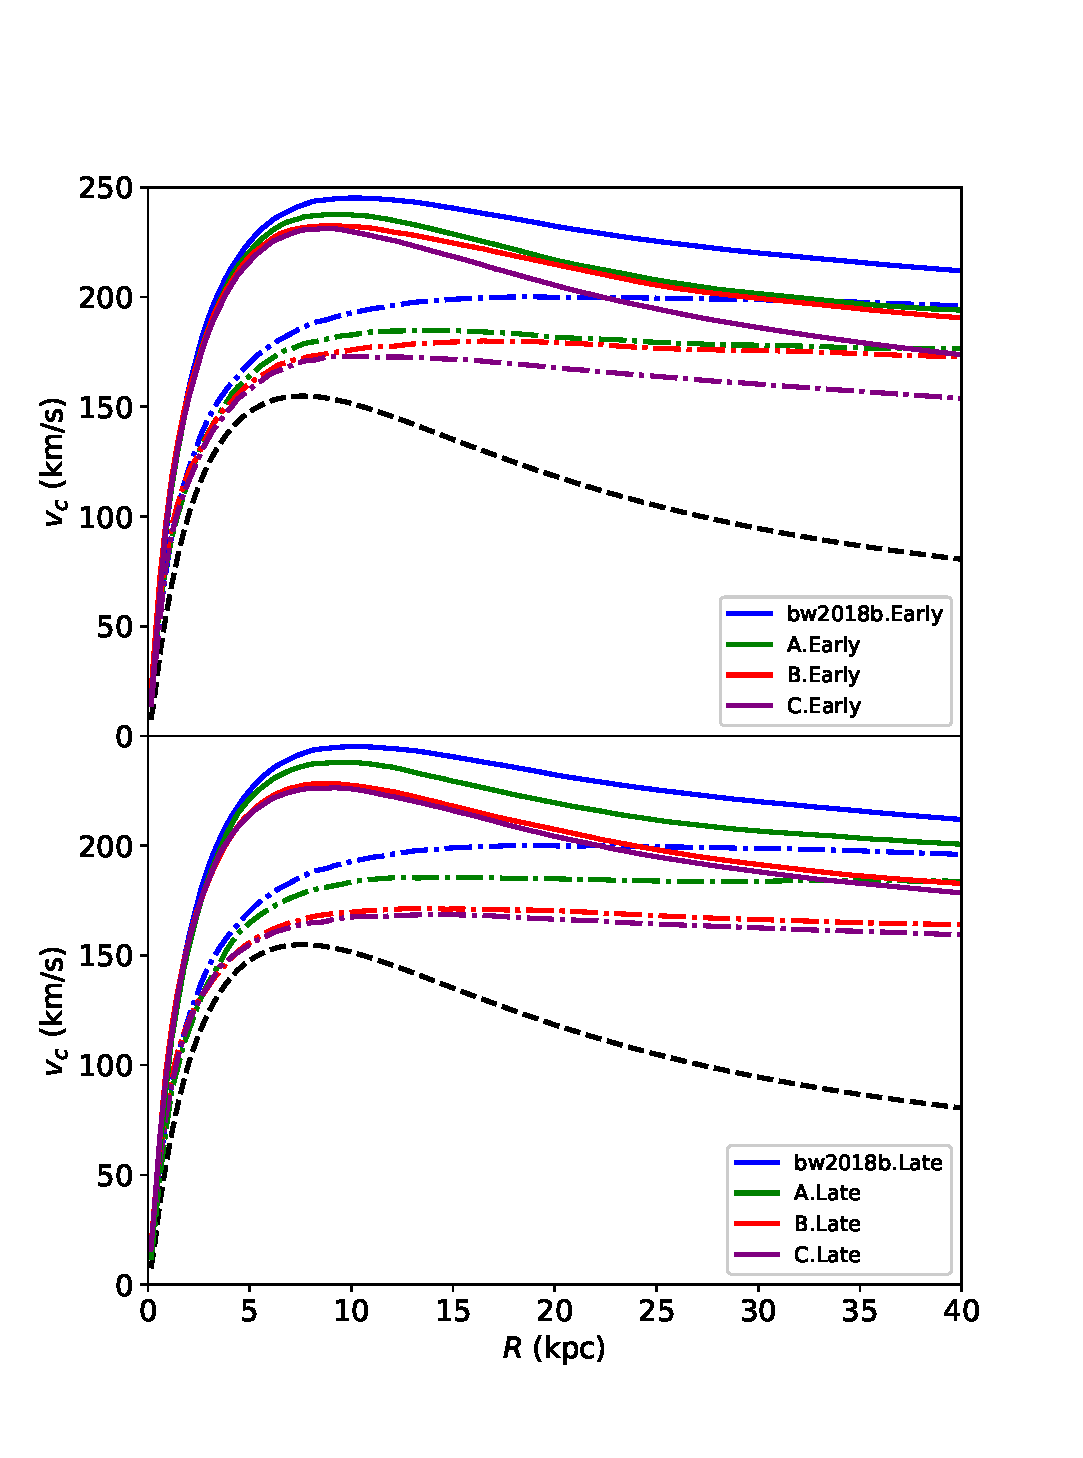
\includegraphics[width=0.85\textwidth]{../figures/rotation_curve.eps}
	\caption{Circular speed curves for cosmological models. The
          same disc is used in all runs, and its rotation curve
          contribution is shown by the black dashed line. The halo
          contributions for the Early and Warm subsuites are shown in
          the top panel as dot-dashed lines, while the total rotation
          curves are shown as solid curves. The bottom panel shows the
          same for the Late subsuite.} \label{fig:rotation_curves_iii}
\end{figure}

\begin{figure}
	\centering
	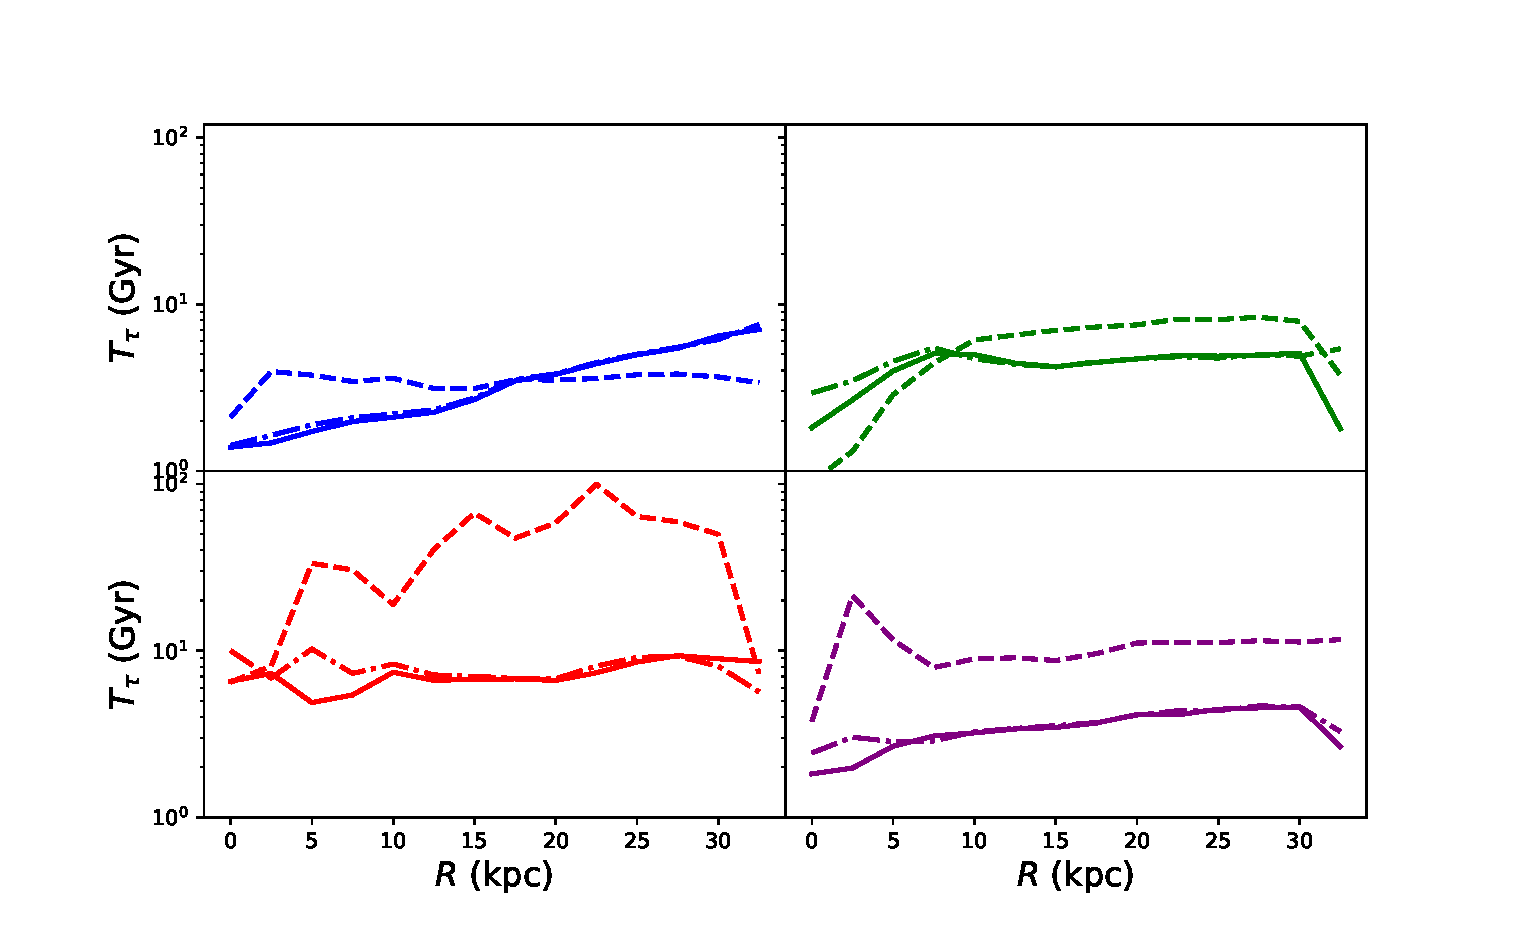
\includegraphics[width=0.85\textwidth]{../figures/timescale.eps}\caption{The
          torque timescale, $T_\tau$, at initialization as a function of $R$.
          Colours are the same as in
          Fig. 5 with bauer2018b in the upper left panel, A in the upper right,
          B in the lower left, and C in the lower right.
          Line types are Early (solid), Warm (dot-dashed), and
          Late (dashed).} \label{fig:ratio_freqs}
\end{figure}

\begin{figure}
	%\centering
	\hspace{-0.75in}
	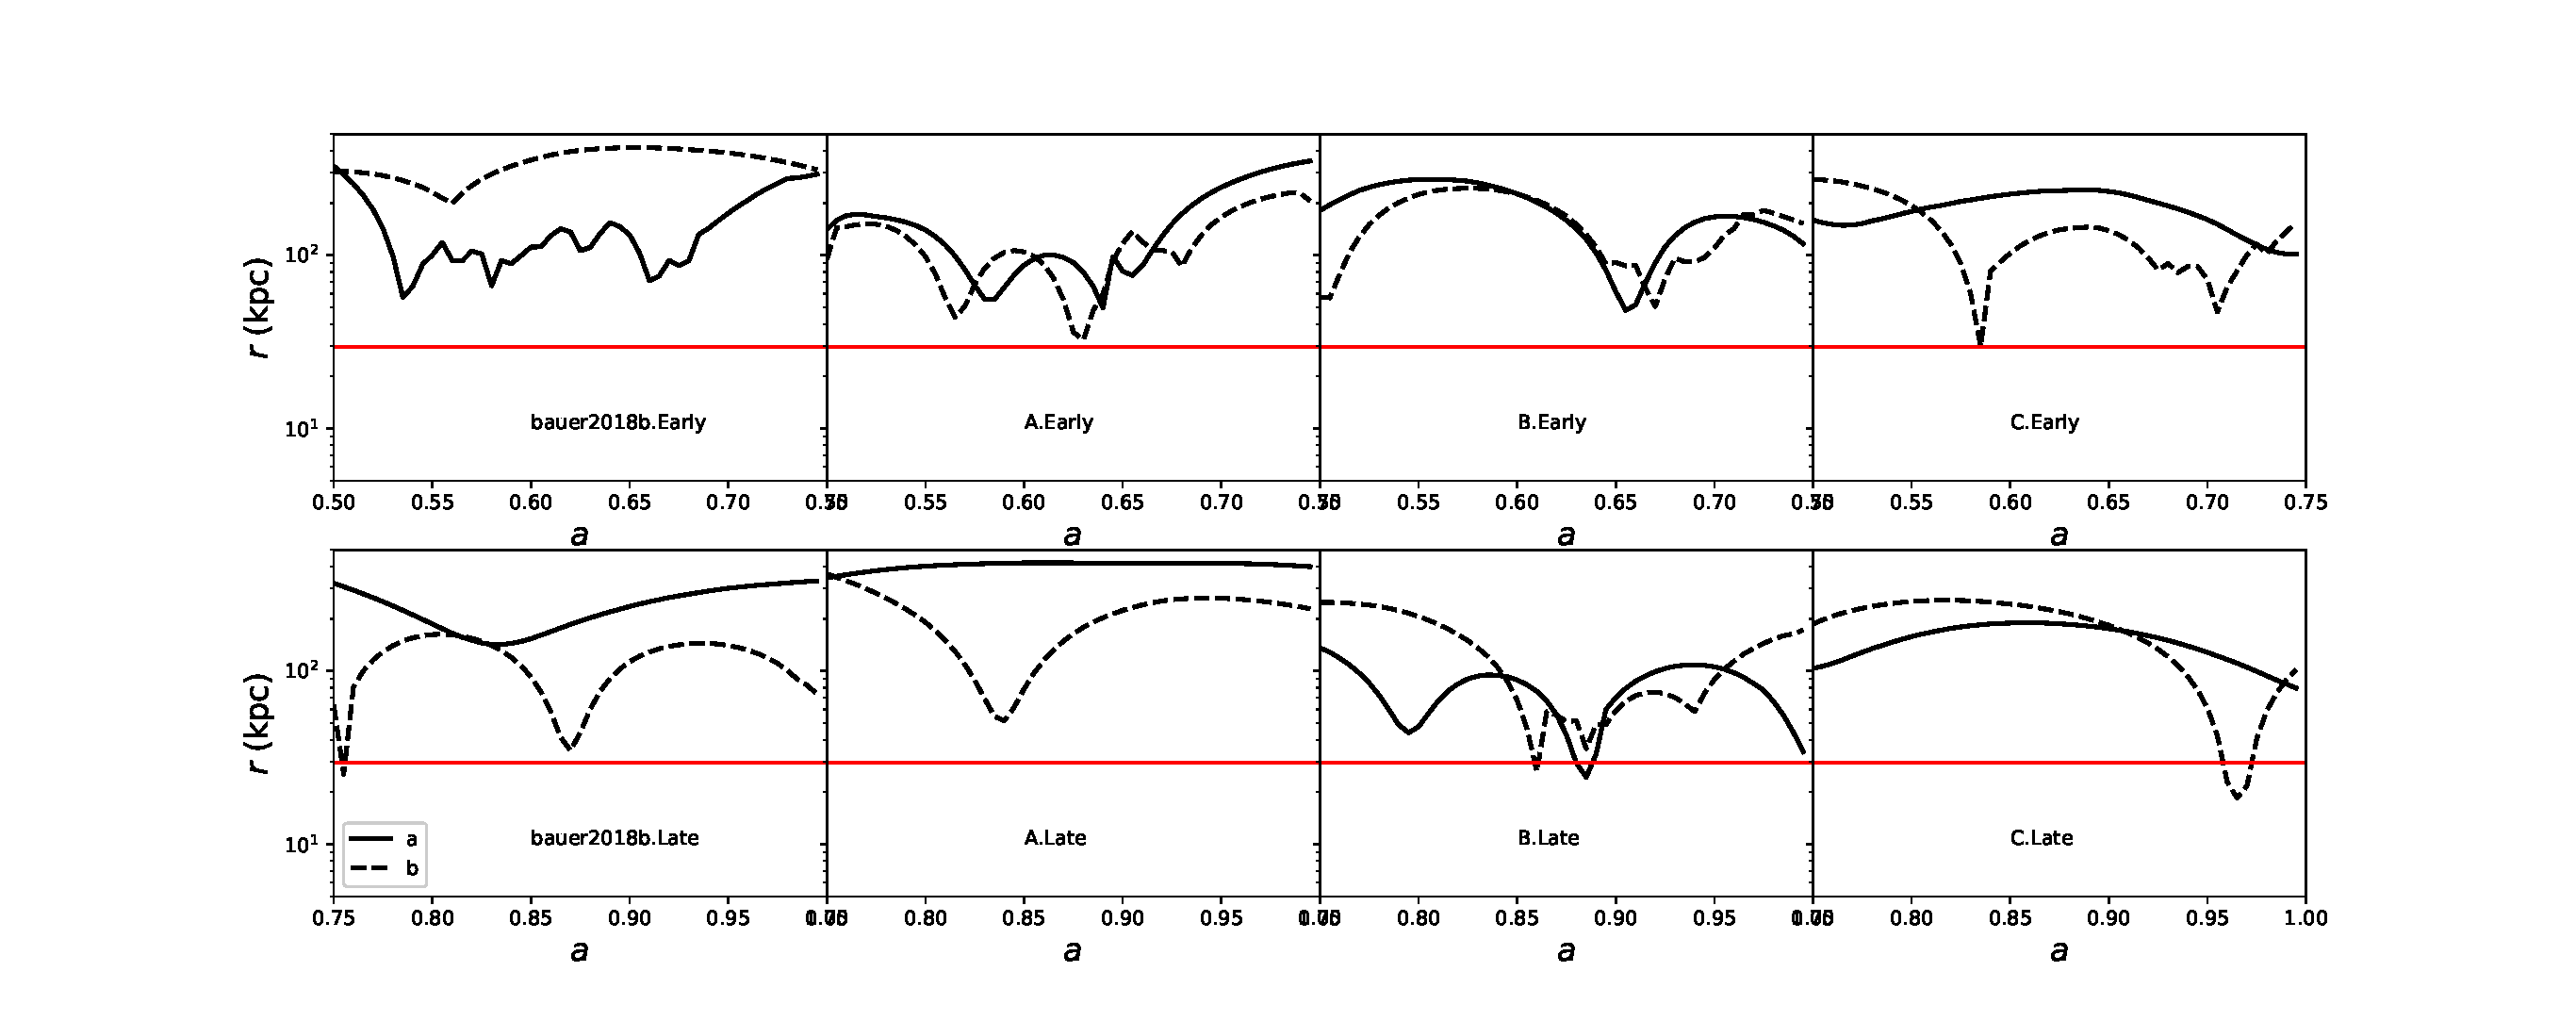
\includegraphics[width=1.2\textwidth]{../figures/substructure_r_vs_t.eps}
	\caption{Orbits of the most massive subhalo (solid curve)
          and second most massive subhalo (dashed curve) for the
          fiducial suite (top panel) and late insertion suite
          (bottom). These are the substructures listed as the top two
          entries for each simulation in Table
          \ref{tab:substructure}. The red line denotes $20\, \kpch =
          29.5 \, \kpc$. } \label{fig:substructure_orbits}
\end{figure}

\subsection{Disc Insertion Technique} \label{ssec:disc_insertio}

Our disc insertion scheme \citep{bauer2018a} expands upon the method
introduced by \citet{BerentzenShlosmanStellarDisks},
\citet{debuhr_2012}, and \citet{ys_2015}. It uses an iterative
procedure to initialize an axisymmetric, smooth disc in a cosmological
halo, that is generally clumpy and triaxial. The first step is to run
a pure dark matter simulation and identify a suitable halo. We then
rerun the simulation with a rigid disc potential that grows from zero
to that of the fully formed disc between an initial scale factor,
$a_g$, to a final scale factor, $a_l$.  When the simulation reaches
$a_l$, the rigid disc is replaced by an N-body system and the ``live''
disc-halo system is evolved to the present epoch at $a=1$.

For our pure dark matter simulation, we implement the zoom-in
technique of \citet{KatzQuasarZoom} and \citet{NavarroWhiteZoom}.  We
select Milky Way-like halos with no major mergers and use the results
of \cite{onorbe_etal_2014} to ensure minimal contamination of
low-resolution particles.  Our choice of cosmological parameters is
based on the results from Planck 2013 \citep{planck_2014}:
$H_0=67.9\,{\rm km\,s}^{-1}\,{\rm kpc}^{-1}$, $\Omega_b = 0.0481$,
$\Omega_0 = 0.306$, $\Omega_\Lambda = 0.694$, $\sigma_8 = 0.827$, and
$n_s = 0.962$. N-body initial conditions for the dark matter particles
are generated with the \textsc{music} code \citep{music}.

During its growth phase from $a_g=0.25$ to $a_l=0.5$\footnote{For
  reference, $a=0.25$ is 2.2 Gyr after the Big Bang, $a=0.5$ is 5.9
  Gyr after the Big Bang, and $a=0.75$ is 10.0 Gyr after the Big
  Bang. The age of this Universe at present day is 13.8 Gyr.}, the
disc is treated as a rigid body whose orientation and center-of-mass
position evolve according to the standard equations of rigid body
dynamics. \citet{bauer2018a} found that the rigid disc assumption is
actually quite true to the orientation and center of mass evolution of
a pure stellar disc. At $a_l$, we swap a live disc for the rigid one
using a modified version of \textsc{GalactICS}
\citep{KGGalactICSReference,WPDGalactICSReference}, which generates a
three-integral DF disc in the best axisymmetric approximation to the
halo \citet{bauer2018a}.

\subsection{Numerical Experiments} \label{ssec:numerical_experiments}

We present a concise description of our cosmological models in Table
\ref{tab:sims_iii}. The haloes are chosen such that the total circular
speed curves are similar to the Milky Way's. Note that the bauer2018b
simulations use a halo from \cite{bauer2018b}. The halos used in the
A, B, and C simulations are previously unpublished.  In the
simulations denoted as X.Early, the disc is inserted at $a_l=0.5$; for
those denoted X.Lake, $a_l=0.75$.  One of the benefits of disc
insertion techniques is the ability to modify disc properties in the
same halo. We exploit this capability in our third suite, denoted as
X.Warm, where we increase the disc's dynamical temperature as
measured by the Toomre $Q$ parameter \citep{toomre_q}.
 
Fig. \ref{fig:rotation_curves_iii} shows the circular speed curves for all
disc-halo combinations. There are relatively small variations in the
circular speed for $R<5\,{\rm kpc}$ where the disc dominates. The
variations are significant ($\sim 10\,{\rm km\,s}^{-1}$) near the peak
of the circular speed curve and even larger beyond the disc where the
halo dominates the gravitational potential. In all cases, the disc is
submaximal. In particular, the ratio of the square of the disc
contribution to the rotation curve and square of the total rotation
curve measured at $2.2\, R_d$, $\left. V_d^2/V_{tot}^2 \right
\vert_{R=2.2\,R_d}$, ranges between 0.37 and 0.46. These values are
well below the lower bound for a maximal disc advocated by
\citet{sackett_1997}.

In the discussion that follow, we focus on three archetypal
simulations:
\begin{enumerate}
\item \textbf{strong disc-subhalo interaction:} In B.Late the disc has close
  interactions with two subhaloes but no substantial disc-halo
  misalignment. One of these subhaloes passes twice through the plane
  of the disc.
\item \textbf{disc-halo misalignment:} C.Early presents a case a
  substantial misalignment from its host halo (see below) but
  relatively modest subhalo interactions with the disc.
\item \textbf{distant massive subhaloes:} The disc in A.Early is relatively
  well aligned to its host halo, but its most massive substructures do not
  interact closely with the disc.
\end{enumerate}

To illustrate how the simulations differ, consider
Fig.\,\ref{fig:torque} where we plot the component of the torque
perpendicular to the spin axis of the disc across the disc plane. In
B.late, we have the localized effect of a subhalo that passes through
the plane of the disc. On the other hand, in C.Early, we have a strong
$m=2$ torque due to the large-scale structure of the halo and
misalignment of the disc with any of the halo's approximate symmetry
axes.

\begin{figure}
	\centering
	\subfloat[]{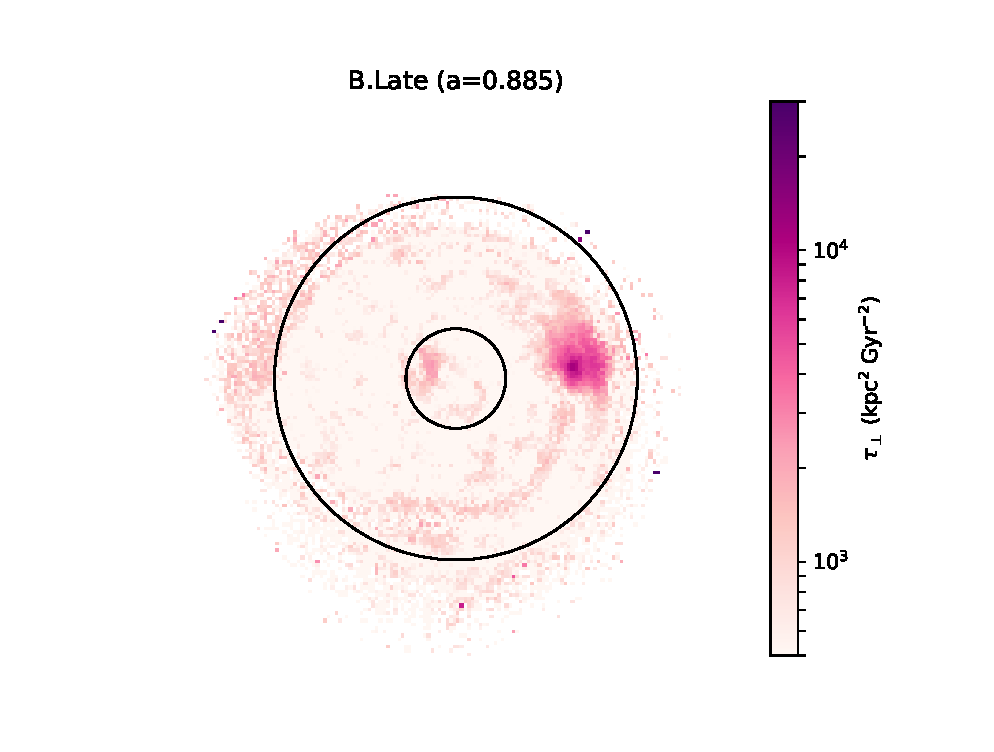
\includegraphics[width=0.8\textwidth]{../figures/b_late_torque_a_0_885.eps}}\\
	\subfloat[]{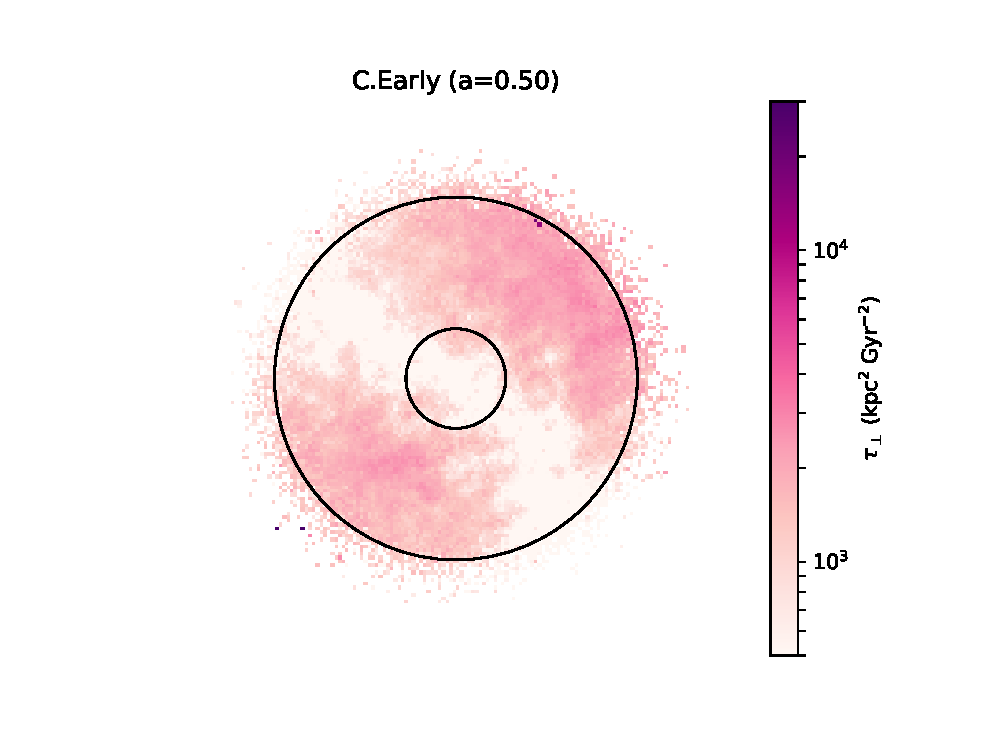
\includegraphics[width=0.8\textwidth]{../figures/c_early_torque_a_0_5.eps}}
	\caption{The component of the torque perpendicular to the spin
          axis of the disc across the disc plane. Top
          panel is for B.Late at $a=0.885$ when the most massive
          subhalo is at pericentre.  The bottom panel is for C.Early
          at initialization ($a=0.5$). The circles correspond to $R_p
          = 2.2\,R_d=8.1\,\kpc$ and
          $20\,\kpch=29.5\,\kpc$.}\label{fig:torque}
\end{figure}

\begin{sidewaystable}
\centering
\caption{Table of simulations run in the main experiment. $M_h$ is the
  virial mass of the host halo, $R_h$ is the NFW scale length of the
  host halo, $c$ is the NFW concentration parameter of the host halo,
  $a_l$ is the live disc insertion scale factor, $\delta
  \Theta_{h,20}$ is the halo misalignment angle for the 20 kpc shell,
  $N_d$ is the number of disc particles, $Q$ is the Toomre stability
  parameter of the disc at initialization, and $f_{kud}$ is the
  fraction of disc mass that gets classified as kicked-out-disk (KOD)
  stars measured at present day with $\eta=8$.} \label{tab:sims_iii}
\begin{tabular}{l l l l l l l l l l}
\hline
       & $M_h\,\,(\solarm)$ & $R_h\,\,(\kpc)$ & $c$ & $a_l$ &  $N_d$ & $Q$ & $\cos\delta \Theta_{h,20}$ & $f_{kud}$\\
\hline
bauer2018.Early   & $1.0 \times 10^{12}$ & 15.9 &  9.84 &   0.50 & $1.0 \times 10^6$ & 1.1 & 0.16 & $1.2 \times 10^{-2}$\\
bauer2018.Warm    & $1.0 \times 10^{12}$ & 15.9 &  9.84 &   0.50 & $1.0 \times 10^6$ & 1.1 & 0.16 & $1.1 \times 10^{-2}$\\
bauer2018.Late    & $1.2 \times 10^{12}$ & 15.2 &  15.4 &   0.75 & $1.0 \times 10^6$ & 1.8 & 0.93 &$4.2 \times 10^{-3}$\\
A.Early           & $9.4 \times 10^{11}$ & 17.8 &  8.56 &   0.50 & $3.5 \times 10^6$ & 1.3 & 0.97 &$3.7 \times 10^{-3}$\\
A.Warm            & $9.4 \times 10^{11}$ & 17.8 &  8.56 &   0.50 & $3.5 \times 10^6$ & 1.8 & 0.97 & $1.6 \times 10^{-3}$\\
A.Late            & $1.1 \times 10^{12}$ & 18.5 &  12.1 &   0.75 & $3.5 \times 10^6$ & 1.3 & 0.98 & $6.8 \times 10^{-5}$\\
B.Early           & $5.9 \times 10^{11}$ & 10.4 &  12.6 &   0.50 & $3.5 \times 10^6$ & 1.3 & 0.91 & $8.5 \times 10^{-4}$\\
B.Warm            & $5.9 \times 10^{11}$ & 10.4 &  12.6 &   0.50 & $3.5 \times 10^6$ & 1.8 & 0.91 & $1.2 \times 10^{-3}$\\
B.Late            & $1.1 \times 10^{12}$ & 33.2 &  6.70 &   0.75 & $3.5 \times 10^6$ & 1.3 & 0.99 & $9.2 \times 10^{-4}$\\
C.Early           & $4.3 \times 10^{11}$ & 8.33 &  14.1 &   0.50 & $3.5 \times 10^6$ & 1.3 & 0.84 & $5.3 \times 10^{-3}$\\
C.Warm            & $4.3 \times 10^{11}$ & 8.33 &  14.1 &   0.50 & $3.5 \times 10^6$ & 1.8 & 0.84 & $5.6 \times 10^{-3}$\\
C.Late            & $6.7 \times 10^{11}$ & 13.6 &  14.0 &   0.75 & $3.5 \times 10^6$ & 1.3 & 0.92 & $1.0 \times 10^{-4}$\\
\hline
\end{tabular} 

\end{sidewaystable}

\subsection{Halo Environments} \label{ssec:halo_env}

To further quantify the effect of the halo environment we define a
torque timescale:
\begin{equation}
T_\tau(R) = \frac{L(R)}{\tau_\perp(R)},
\end{equation}
where $L(R)$ is the magnitude of the angular momentum in a ring
centered at radius $R$ and $\tau_\perp(R)$ is the azimuthally-averaged
component of the torque that is perpendicular to the spin axis of the
disc.  The greater the misalignment between disc and halo, the larger
the torque of the halo on the disc, and the shorter the timescale
$T_\tau$. In Fig. \ref{fig:ratio_freqs}, we plot $T_\tau$ as a
function of radius at initialization for our models. In general, the
effect of tidal torques from the halo are smaller at late times when
much of the substructure and triaxiality of the halo has been washed
out. We also infer that the effect of the halo in torquing the disc is
largest in C.Early.

In Table \ref{tab:substructure}, we list the five most massive (at
initialization) substructures for each of our simulations while the
orbits of the two most massive substructures are shown in
Fig. \ref{fig:substructure_orbits}.  The orbits present a wide variety
of behaviour. For example, the subhaloes in bauer2018b.Early spend
most of their lives in the outer halo on roughly tangential orbits. By
contrast, the second most mass subhalo in C.late orbits to within
$\sim 20\,{\rm kpc}$ of the disc centre. The subhalos in A.early are
more massive but never reach to within $30\,{\rm kpc}$.

\begin{sidewaystable}
\caption{Table of the five most massive substructures at $a_l$ in all
  of the simulations detailed in Table \ref{tab:sims_iii}. The virial
  mass, $M_s$, and NFW scale radius, $R_s$, are
  given.}\label{tab:substructure}
	\begin{tabular}{|l l l l | l l l l|}
	\hline
	Subhalo Name ($z=1$) & $M_s \,(\solarm)$ & $R_s \, (\kpc)$ & $c$ & Subhalo Name ($z=0.333$) & $M_s \,(\solarm)$ & $R_s \, (\kpc)$ & $c$\\	
	\hline
    bauer2018b.Early.a & $1.4 \times 10^{10}$ & 3.75 & 9.92 & bauer2018b.Late.a & $1.6 \times 10^{10}$ & 3.35 & 16.5 \\
    bauer2018b.Early.b & $1.0 \times 10^{10}$ & 1.02 & 32.8 & bauer2018b.Late.e & $0.7 \times 10^{10}$ & 0.27 & 154. \\
    bauer2018b.Early.c & $0.5 \times 10^{10}$ & 2.60 & 10.1 & bauer2018b.Late.c & $0.3 \times 10^{10}$ & 0.07 & 485. \\
    bauer2018b.Early.d & $0.4 \times 10^{10}$ & 1.51 & 15.7 & bauer2018b.Late.d & $0.3 \times 10^{10}$ & 1.06 & 29.8 \\
    bauer2018b.Early.e & $0.2 \times 10^{10}$ & 0.28 & 69.0 & bauer2018b.Late.e & $0.2 \times 10^{10}$ & 0.38 &  76.7\\
	\hline
	A.Early.a & $1.8 \times 10^{10}$ & 2.69 & 15.3 & A.Late.a & $1.3 \times 10^{10}$ & 2.62 & 19.6 \\
	A.Early.b & $1.2 \times 10^{10}$ & 1.26 & 28.4 & A.Late.b & $0.9 \times 10^{10}$ & 0.61 & 74.8 \\
	A.Early.c & $1.0 \times 10^{10}$ & 0.71 & 47.9 & A.Late.c & $0.5 \times 10^{10}$ & 0.77 & 46.4 \\
	A.Early.d & $0.7 \times 10^{10}$ & 2.29 & 13.0 & A.Late.d & $0.4 \times 10^{10}$ & 1.69 & 19.7 \\
	A.Early.e & $0.5 \times 10^{10}$ & 1.73 & 13.2 & A.Late.e & $0.2 \times 10^{10}$ & 1.25 & 21.5 \\
	\hline
	B.Early.a & $1.1 \times 10^{10}$ & 1.76 & 19.4 & B.Late.a & $2.7 \times 10^{10}$ & 1.70 & 38.1 \\
	B.Early.b & $0.2 \times 10^{10}$ & 0.41 & 47.5 & B.Late.b & $1.2 \times 10^{10}$ & 2.27 & 22.0 \\
	B.Early.c & $0.2 \times 10^{10}$ & 0.67 & 28.4 & B.Late.c & $0.6 \times 10^{10}$ & 2.67 & 14.4 \\
	B.Early.d & $0.2 \times 10^{10}$ & 1.81 & 10.3 & B.Late.d & $0.4 \times 10^{10}$ & 1.42 & 24.0 \\
	B.Early.e & $0.2 \times 10^{10}$ & 0.54 & 34.0 & B.Late.e & $0.4 \times 10^{10}$ & 1.13 & 29.7 \\
	\hline
    C.Early.a & $1.0 \times 10^{10}$ & 1.78 & 18.5 & C.Late.a & $0.5 \times 10^{10}$ & 0.18 & 194. \\
	C.Early.b & $0.6 \times 10^{10}$ & 0.92 & 30.0 & C.Late.b & $0.4 \times 10^{10}$ & 6.37 & 5.46 \\
	C.Early.c & $0.3 \times 10^{10}$ & 2.24 & 10.2 & C.Late.c & $0.4 \times 10^{10}$ & 0.75 & 46.2 \\
	C.Early.d & $0.1 \times 10^{10}$ & 0.91 & 18.7 & C.Late.d & $0.3 \times 10^{10}$ & 1.26 & 26.1 \\
	C.Early.e & $0.1 \times 10^{10}$ & 0.25 & 60.3 & C.Late.e & $0.3 \times 10^{10}$ & 6.78 & 4.81 \\
	\hline
	\end{tabular}
\end{sidewaystable}

\section{Structure and Evolution of Simulation Models} \label{sec:evolution}

In this section we summarize the evolution of the models in our
simulations.  We begin with a discussion of bar formation and then
turn to bending and warping of the discs.

\subsection{Bar Formation}

\begin{figure}
    \centering
    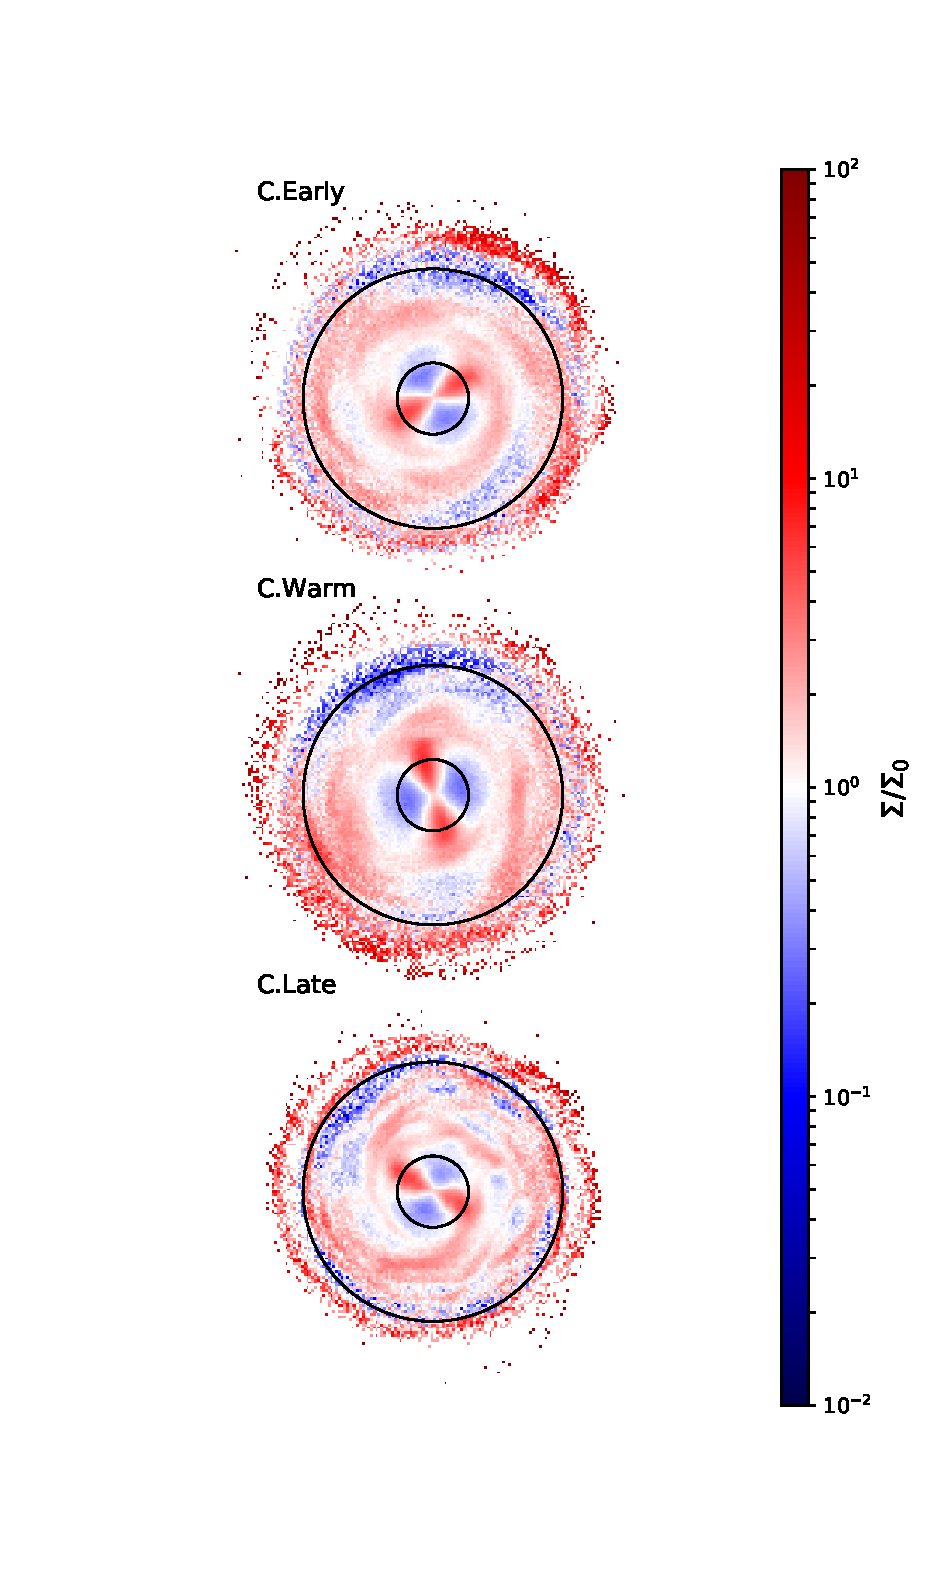
\includegraphics[width=0.7\textwidth]{../figures/surface_density_ratios.eps} \caption{The
      ratio of surface density, $\Sigma$, to azimuthally averaged
      surface density, $\Sigma_0$ for the C.Early, C.Warm, and C.Late
      models. The circles correspond to $R_p = 2.2\, R_d = 8.1 \,\kpc$
      and $20 \,\kpch = 29.5 \, \kpc$.}
	\label{fig:final_densities}
\end{figure}

\begin{figure}
	\centering
	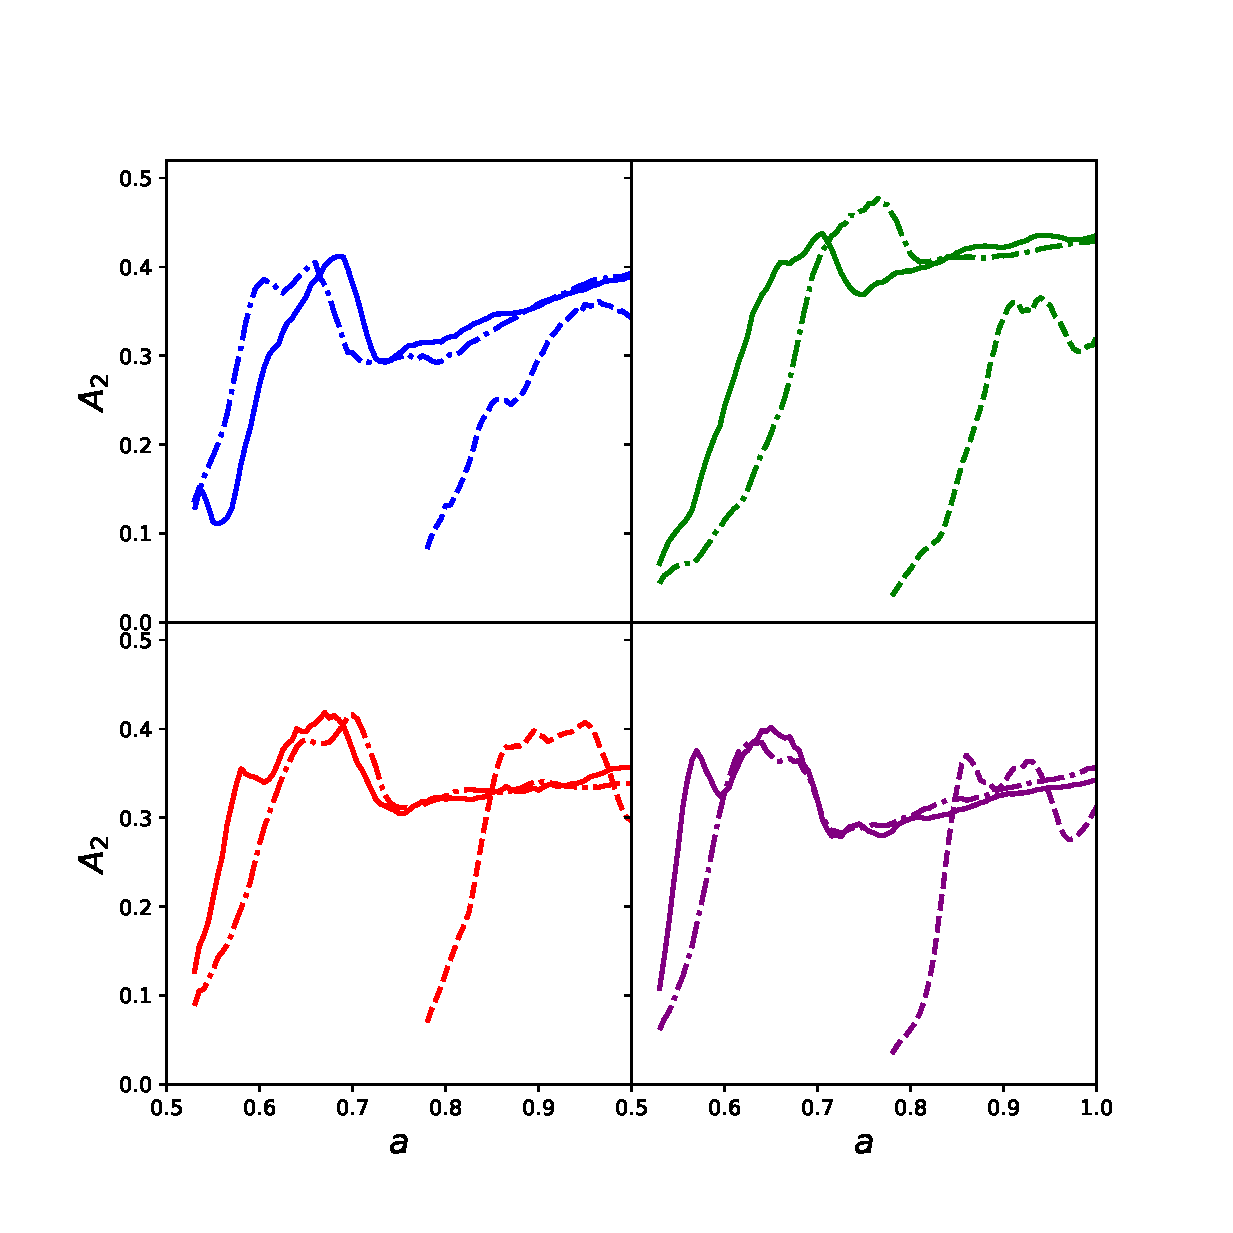
\includegraphics[width=0.85\textwidth]{../figures/a_2_all_models_four_panel.eps}
	\caption{Bar strength as measured by $A_2(<R_p)$ as a function of time for all models.} \label{fig:a_2}
\end{figure}

In isolation, a disc-halo system forms a bar when $m=2$ {density} instabilities,
seeded by shot noise-induced perturbations, exponentially grow
\citep{EfstathiouShotNoise}. Factors such as the relative contribution
of the disc to the rotation curve, radial velocity dispersion, and the
disc scale height broadly determine formation rate, strength, and
length of the bar
\citep{AthanassoulaSellwood1986,ChristodoulouStability1995,
  Klypin2009, Sellwood2013, bauer2018b}.  Strong environmental
perturbers such as halo substructure and tides can induce bar
formation even in discs that resist bar formation in isolation
\citep{gauthier_2006, kazantzidis2008, purcell2011}.

\citet{debuhr_2012,ys_2015} used a disc insertion scheme similar to
the one used here and found that in the absence of a classical bulge
stellar discs always formed bars in a cosmological environment, even
if they are submaximal.  In a previous paper, we argued that these
simulations overestimated the susceptibility of a disc to forming
strong bars \citep{bauer2018b}. This argument stems from the
observation that the discs in \citet{debuhr_2012} and \citet{ys_2015}
were too thick by a factor of $\sim 2$ as compared with the thickness
of the Milky Way and similar galaxies. We found that the more
realistic thin discs grow bars more quickly that then buckle. Since
buckling regulates the strength of the bar, the net result is that
bars in thin discs end up being weaker than those in thick discs
\citep{Klypin2009,bauer2018b}.

In Fig. \ref{fig:final_densities} we show the ratio of the surface
density across the face of the disc to the azimuthally-averaged
surface density for the final snapshots of the C.Early, C.Warm,
and C.Late simulations. Similar results are obtained for the
bauer2018, A, and B simulations. Bars form in all three simulations,
as evidenced by the X-pattern at the centre of the disc. The bar
connects with a two-armed spiral in C.Early and C.Late. The 
bar-spiral arm connection is less obvious in the C.Warm simulation.

In Fig. \ref{fig:a_2}, we plot the bar strength parameter {($\Theta=1$ in Eq. \eqref{eq:z_statistic})} evaluated in
the region $R < 2.2 R_p$ \citep{debattista_sellwood_2000}. We see that
all models experience some kind of buckling event, which reduces $A_2$
by $20-30\%$.  With the exception of bauer2018b, bar formation and
buckling is delayed in the warm disc simulations relative to the cold
disc ones.

Broadly speaking, our simulations form bars similar to that of the
Milky Way's bar in strength and length. The bulk of the bar mass in
all simulations appears contained to within $R_p = 2.2\, R_d$ The
late-insertion suite shows a reduced bar length, bolstering an idea
presented in \citet{bauer2018b} that for similar galaxies, one might
be able to use the bar length to compare relative ages of stellar
discs.

\subsection{Disc Heating}
\begin{figure}
	\centering
	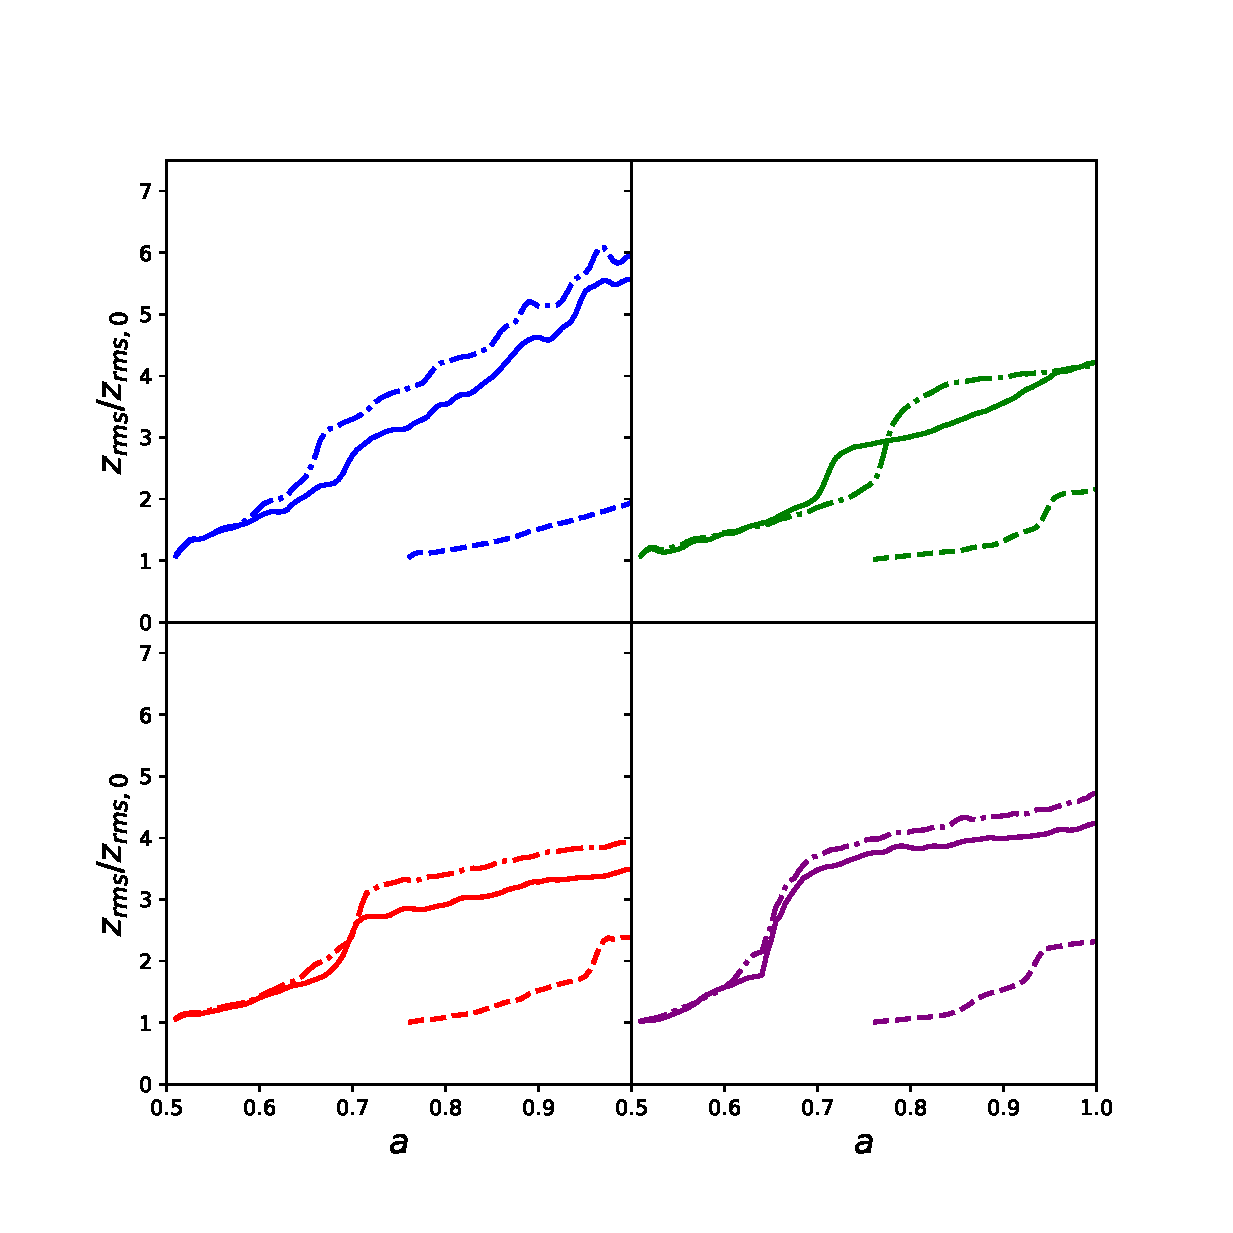
\includegraphics[width=0.85\textwidth]{../figures/z_rms_all_models_four_panel.eps}
	\caption{Disc height as measured by $z_{rms}/z_{rms,0}$ as a function of time for all models.} \label{fig:z_rms}
\end{figure}

Vertical heating and thickening in stellar discs is a well-studied
phenomenon, which can be driven by bars and spiral structure
\citep{mcmillan_dehnen_2007,Sellwood2013} or by interactions of the
disc with its satellites and its dark halo \citep[for
  example]{lacey_ostriker_1985, toth_ostriker_1992, sellwood_1998,
  bauer2018b}. These effects suggest that disc in a cosmological
environment should thicken with time, and indeed, this is confirmed in
our simulations.  Fig. \ref{fig:z_rms} shows the evolution of
$z_{rms}$ for each disc in the fiducial and warm suites. We see that
substantial heating follows bar buckling in each simulation, a result
consistent with \citet{gauthier_2006, kazantzidis2008,
  ys_2015,bauer2018b}. We note that the warm suite exhibits up to 25\%
more disc heating. There is little to say about disc heating in the
late-insertion simulations except that the discs approximately double
in thickness over the simulation time. These simulations end as the
buckling is just beginning.

\subsection{Bending waves in Cosmological Discs}

\begin{figure*}
    \centering
    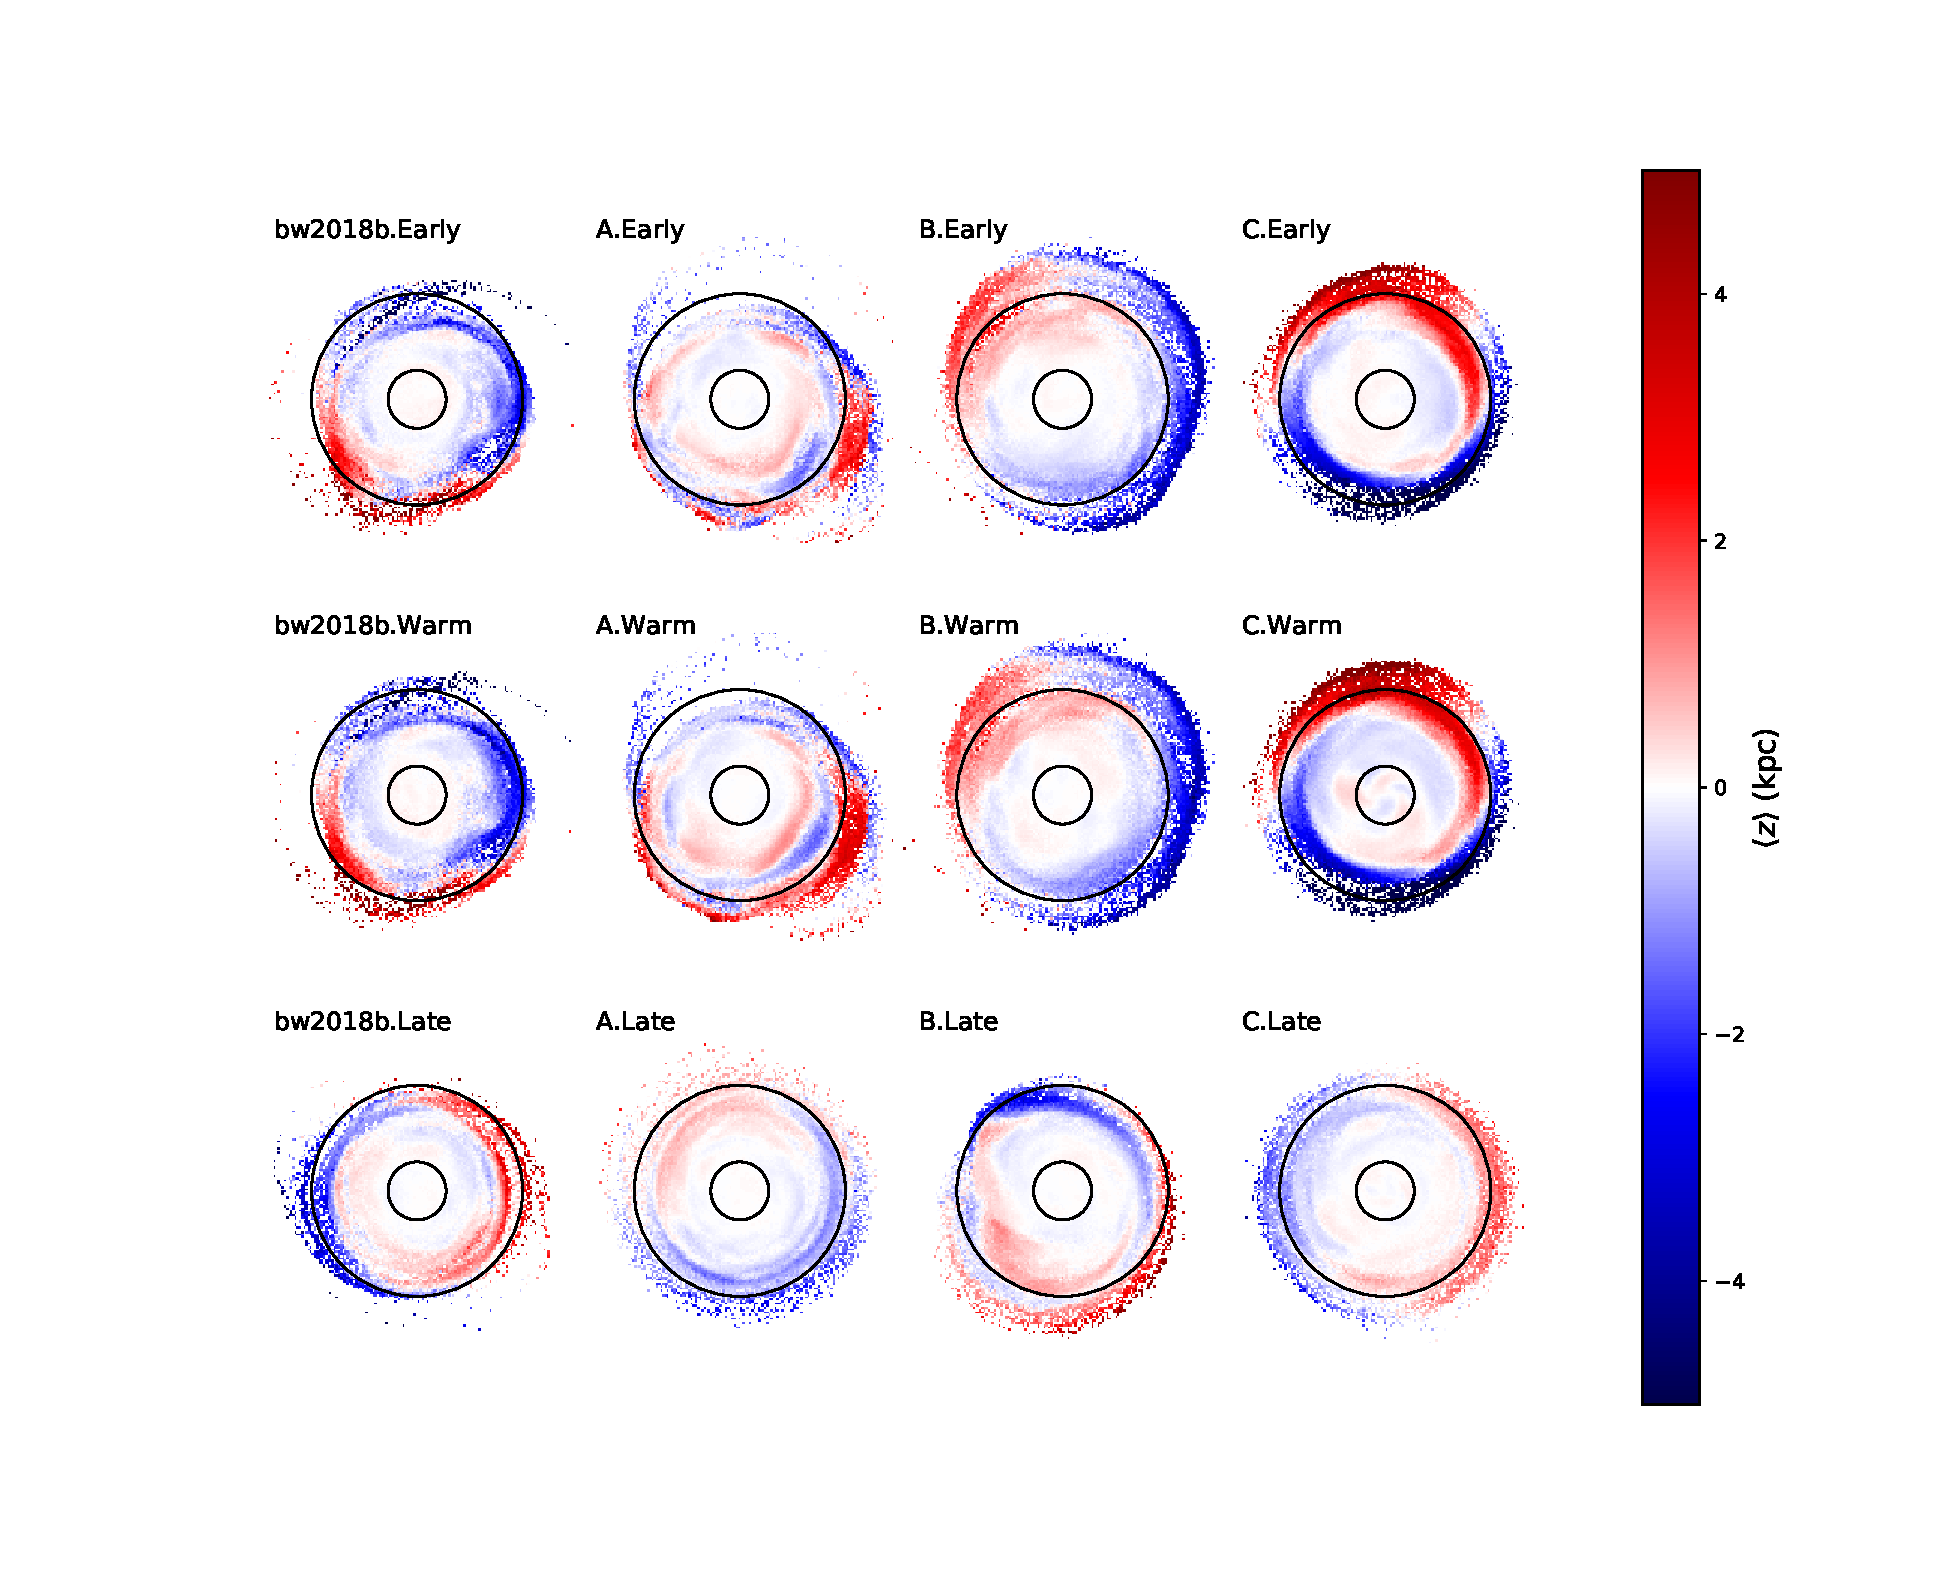
\includegraphics[width=0.9\textwidth]{../figures/twelve_panel_displacements_025.eps}
\caption{Mean displacement above or below the disc at $a=0.625$ for
  the top two rows, and $a=0.875$ for the bottom row (late-insert
  suite). The circles correspond to $2.2 \,R_d = 8.1\,\kpc$ and $20 \,
  \kpch = 29.5\,\kpc$.  }
	\label{fig:vertical_displacement_map}
\end{figure*}

\begin{figure}
	\centering
	\subfloat[]{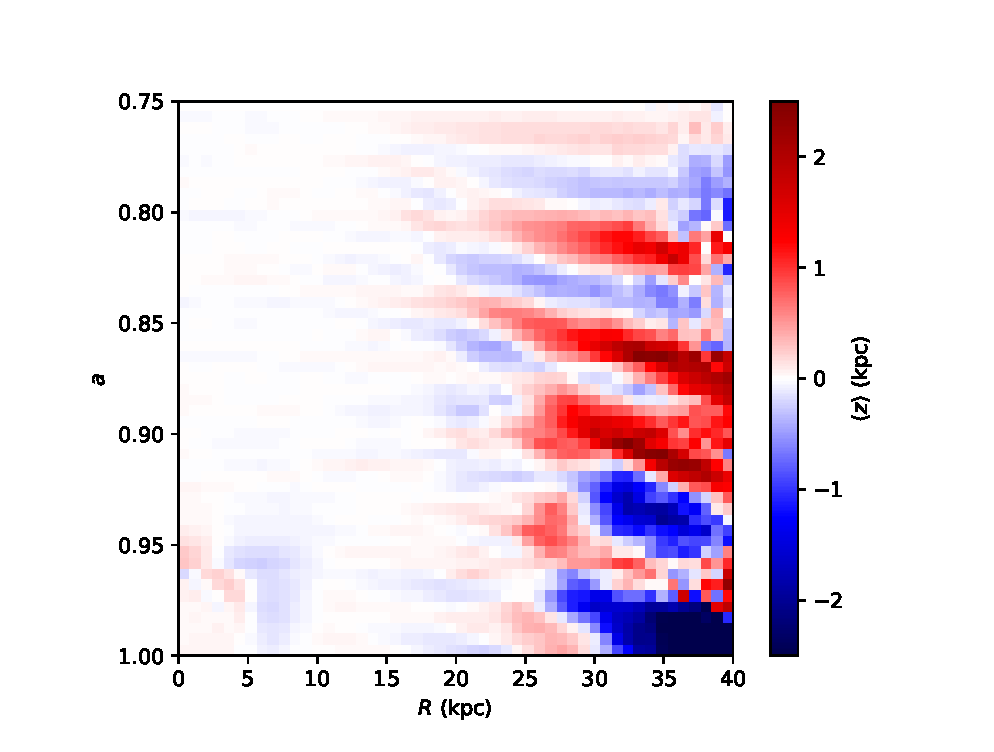
\includegraphics[width=0.45\textwidth]{../figures/b_late_z_0_r_a.eps} \label{fig:b_late_r_a}}
	\subfloat[]{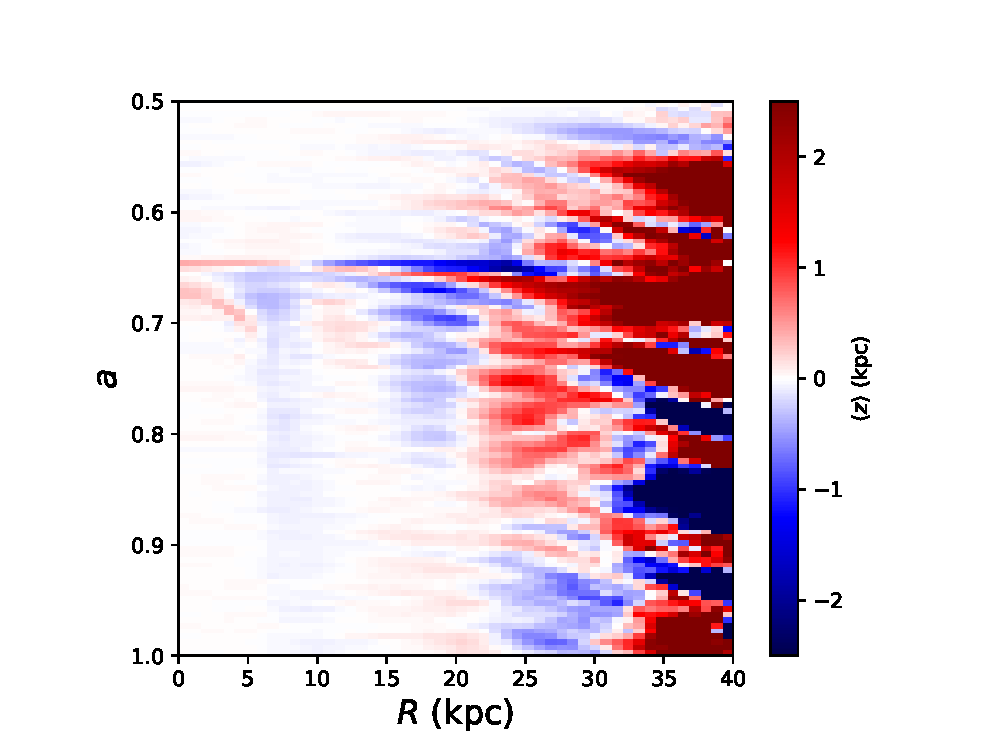
\includegraphics[width=0.45\textwidth]{../figures/c_early_z_0_r_a.eps} \label{fig:c_early_r_a}}\\
	\subfloat[]{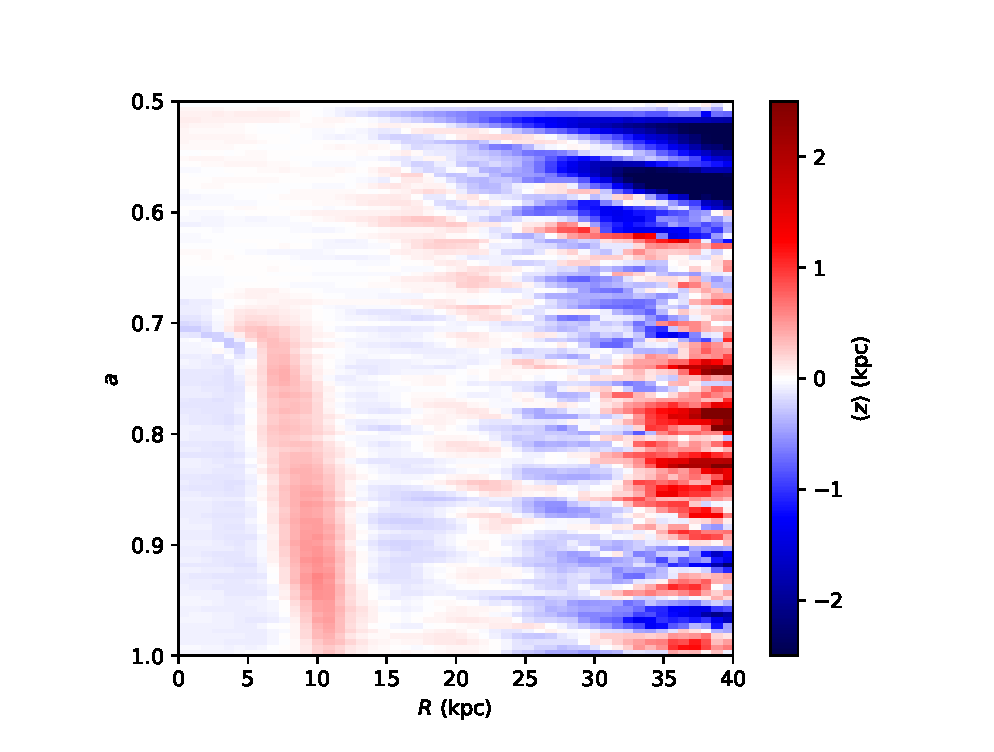
\includegraphics[width=0.45\textwidth]{../figures/a_early_z_0_r_a.eps} \label{fig:a_early_r_a}}	
\caption{The $m=0$ bending mode for B.Late (a), C.Early (b), and
  A.Early (c) as a function of radius and scale factor. }\label{fig:bendingm0}
\end{figure}

\begin{figure}
	\centering
	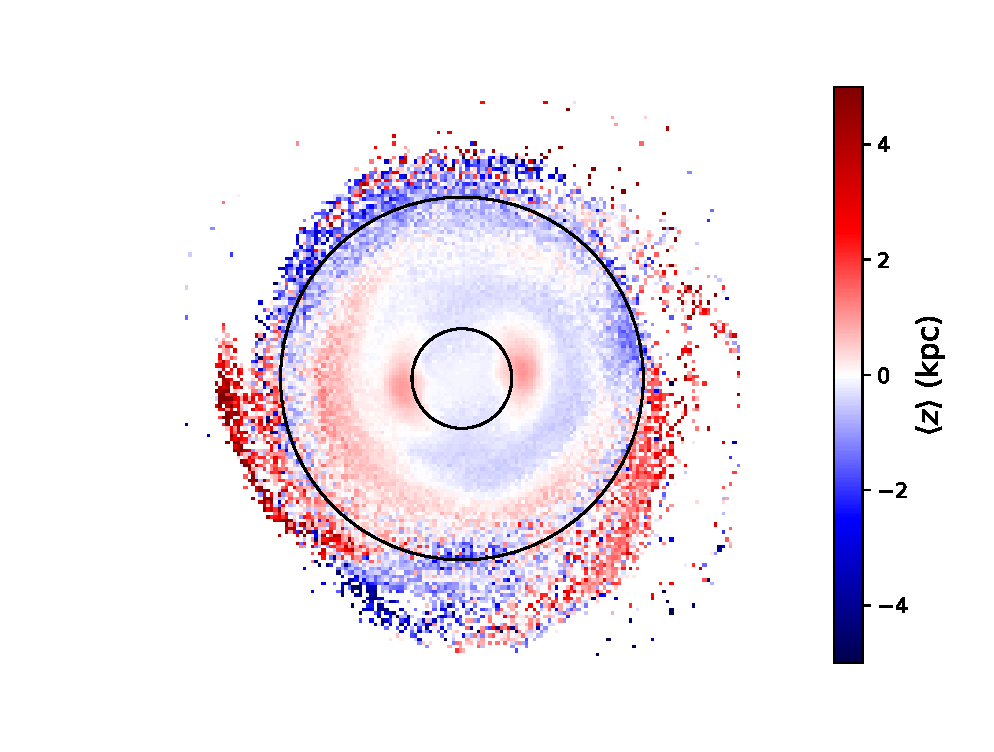
\includegraphics[width=0.85\textwidth]{../figures/a_early_displacement_a_0_875.eps}
	\caption{The mean height, $\langle z \rangle$, map for A.Early at $a=0.875$.}\label{fig:a_early_displacement}
\end{figure}

\begin{figure}\label{fig:binding_m1}
	\centering
	\subfloat[]{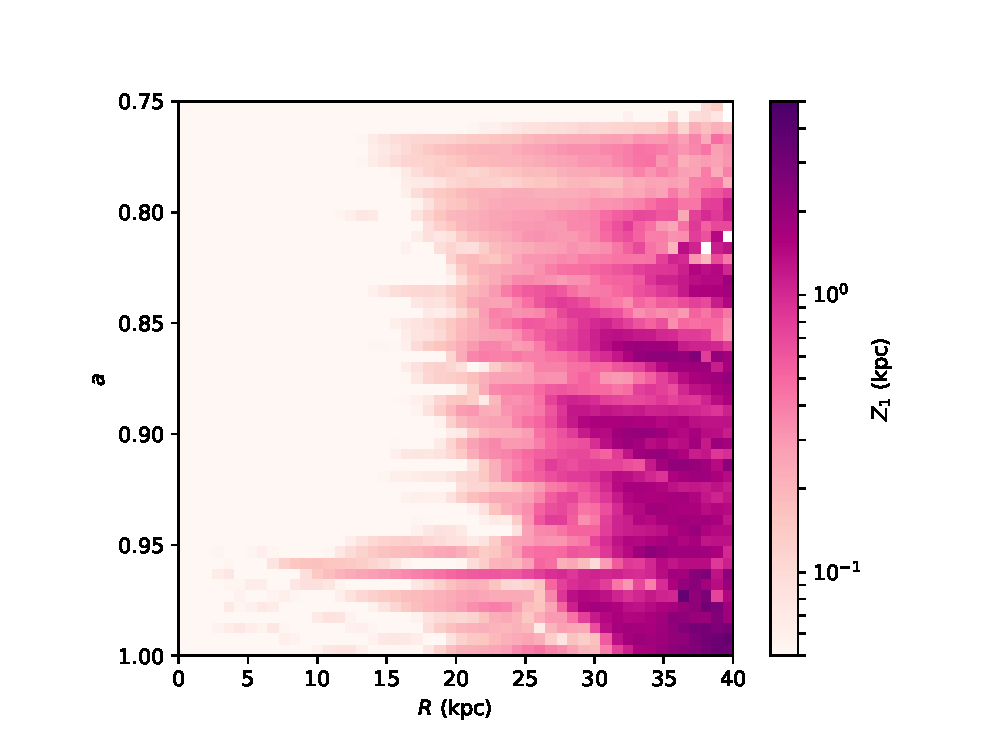
\includegraphics[width=0.45\textwidth]{../figures/b_late_z_1_r_a.eps} \label{fig:b_late_r_a_1}} \subfloat[]{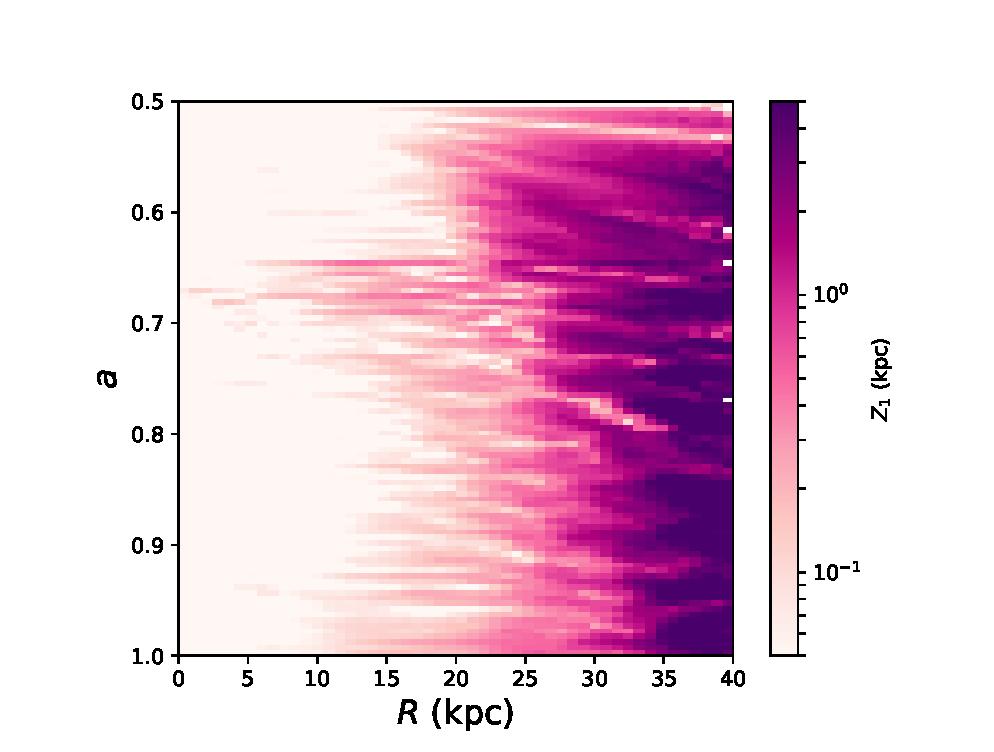
\includegraphics[width=0.45\textwidth]{../figures/c_early_z_1_r_a.eps} \label{fig:c_early_r_a_1}}\\ \subfloat[]{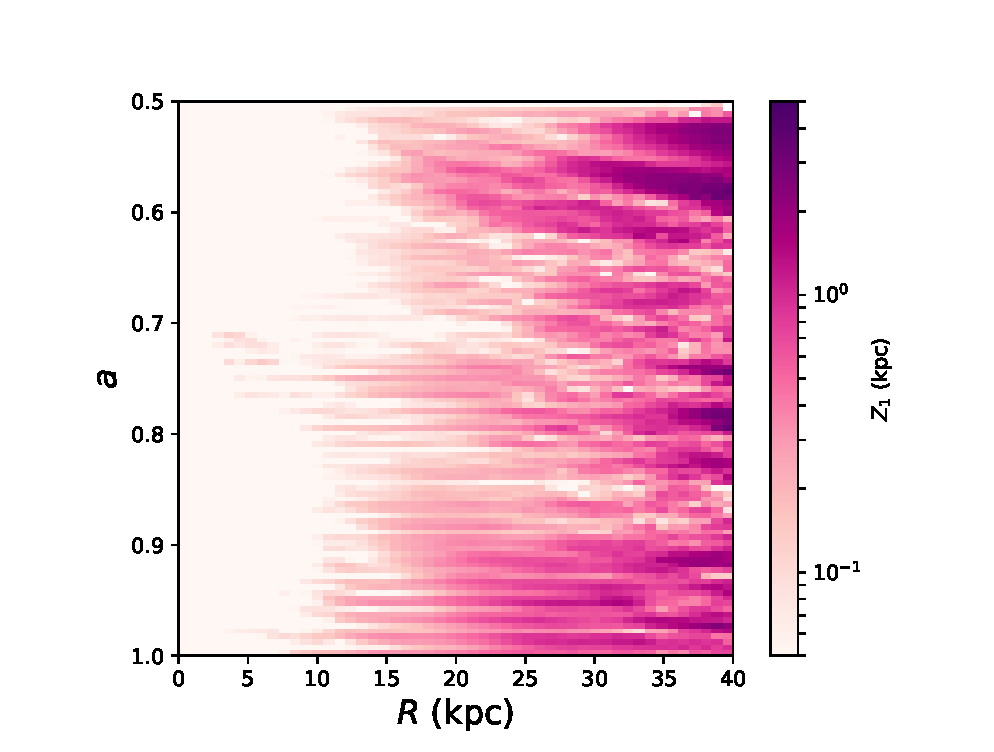
\includegraphics[width=0.45\textwidth]{../figures/a_early_z_1_r_a.eps} \label{fig:a_early_r_a_1}} \caption{The
          $m=1$ bending mode for B.Late (a), C.Early (b), and A.Early
          (c) as a function of radius and scale factor. }
\end{figure}

In Fig. \ref{fig:vertical_displacement_map} we show mean vertical
displacement ($\langle z\rangle$) maps for a single snapshot for our
twelve simulations. We choose $a=0.625$ for the early insertion runs
and $a=0.875$ for the late insertion runs. Significant warping in the
outer discs with midplane displacements of a few kiloparsecs is seen
in all simulations. However, the morphology of the warps varies
considerably. The C and bauer2018b simulations show a clear $m=1$
pattern, while the pattern in A and B is more complicated. Though the
strongest bending features are beyond $20\,{\rm kpc}$ there is clear
evidence for bending waves with amplitudes below 1 kiloparsec further
in.

In Fig.\,\ref{fig:bendingm0} we show the azimuthally-averaged ($m=0$)
bending of the disc as a function of radius and time for three of our
simulations. The B.Late simulation, where a satellite similar to the
Sgr dSph interacts with the disc shows a pattern of bending waves
similar to what we saw in the toy model presented in
\S\ref{ssec:toy_model_2} Monoceros-scale fluctuations interior to
$20\,{\rm kpc}$ occur early on and persist throughout the entire
simulation.

The evolution of $\langle z\rangle(R)$ is rather different in the
C.Early simulation, where disc-halo misalignment is driving the dynamics.
In this case, the bending waves are more like standing waves
(horizontal rather than sloping down and to the right). In addition,
there are bending waves extending all the way to the centre of the
disc, beginning when $a\simeq 0.65$. We attribute these waves the
the buckling of the bar.

Finally, we consider A.Early where the disc interacts with a
relatively massive but more distant subhalo. Bending waves set up in
the outer disc almost immediately while sub-kiloparsec corrugations
persist throughout the disc over the entire simulation. Moreover, at
$a=0.5$ a long-lived feature develops in the inner disc. To explore
this model further, we show a face-on vertical displacement map in Fig.
\ref{fig:a_early_displacement} for $a=0.875$. We interpret this feature
as a 'banana bar', that is, a bar that exibits a permanent bend along
its long axis.

In addition to flapping $m=0$ modes, we detect strong $m=1$ warp
signatures {($\Theta = z$ in Eq. \eqref{eq:z_statistic})} in our three detailed examples. In the case of the strong
satellite encounter, B.Late, we see a sub-kpc warp present in
Fig.\,\ref{fig:b_late_r_a_1} during the first half of the
simulation. As the substructure orbit continues, a close pass excites
stronger $m=1$ structures. In contrast, the strong misalignment case,
C.Early show  in Fig.\,\ref{fig:c_early_r_a_1}, exhibits kiloparsec-scale $m=1$ bending modes in the outer
disc. Furthermore, the strong $m=1$ signal extends inside of 25 kpc at
the beginning of the simulation where there is relatively little $m=0$
signature, and also where B.Late has relatively low $m=1$ signal. The
contour of the $m=1$ bending mode post-buckling roughly traces the
$m=0$ contour with a similar magnitude, suggesting a superposition of
effects brought on by the environment's coupling to the buckling
event.

The intermediate case, A.Early shown in Fig.\,\ref{fig:a_early_r_a_1}, presents something qualitatively
between B.Late and C.Early. While the outer disc is initially excited,
this behaviour subsides as the halo equilibrates. We then find
consistent, several hundred pc signal in the inner and outer disc over
the simulation. Lastly, buckling has a less drastic impact on the
$m=1$ signature for A.Early than it did for the $m=0$.

\section{KOD Dynamics} \label{sec:kud}

In this section, we focus on stars that are kick out of the disc.
We begin with a definition of a KOD star and then discuss the 
kicked-out populations in our simulations.

\subsection{Definition of a KOD star} \label{ssec:def}

\begin{figure*}
    \centering
    \subfloat[]{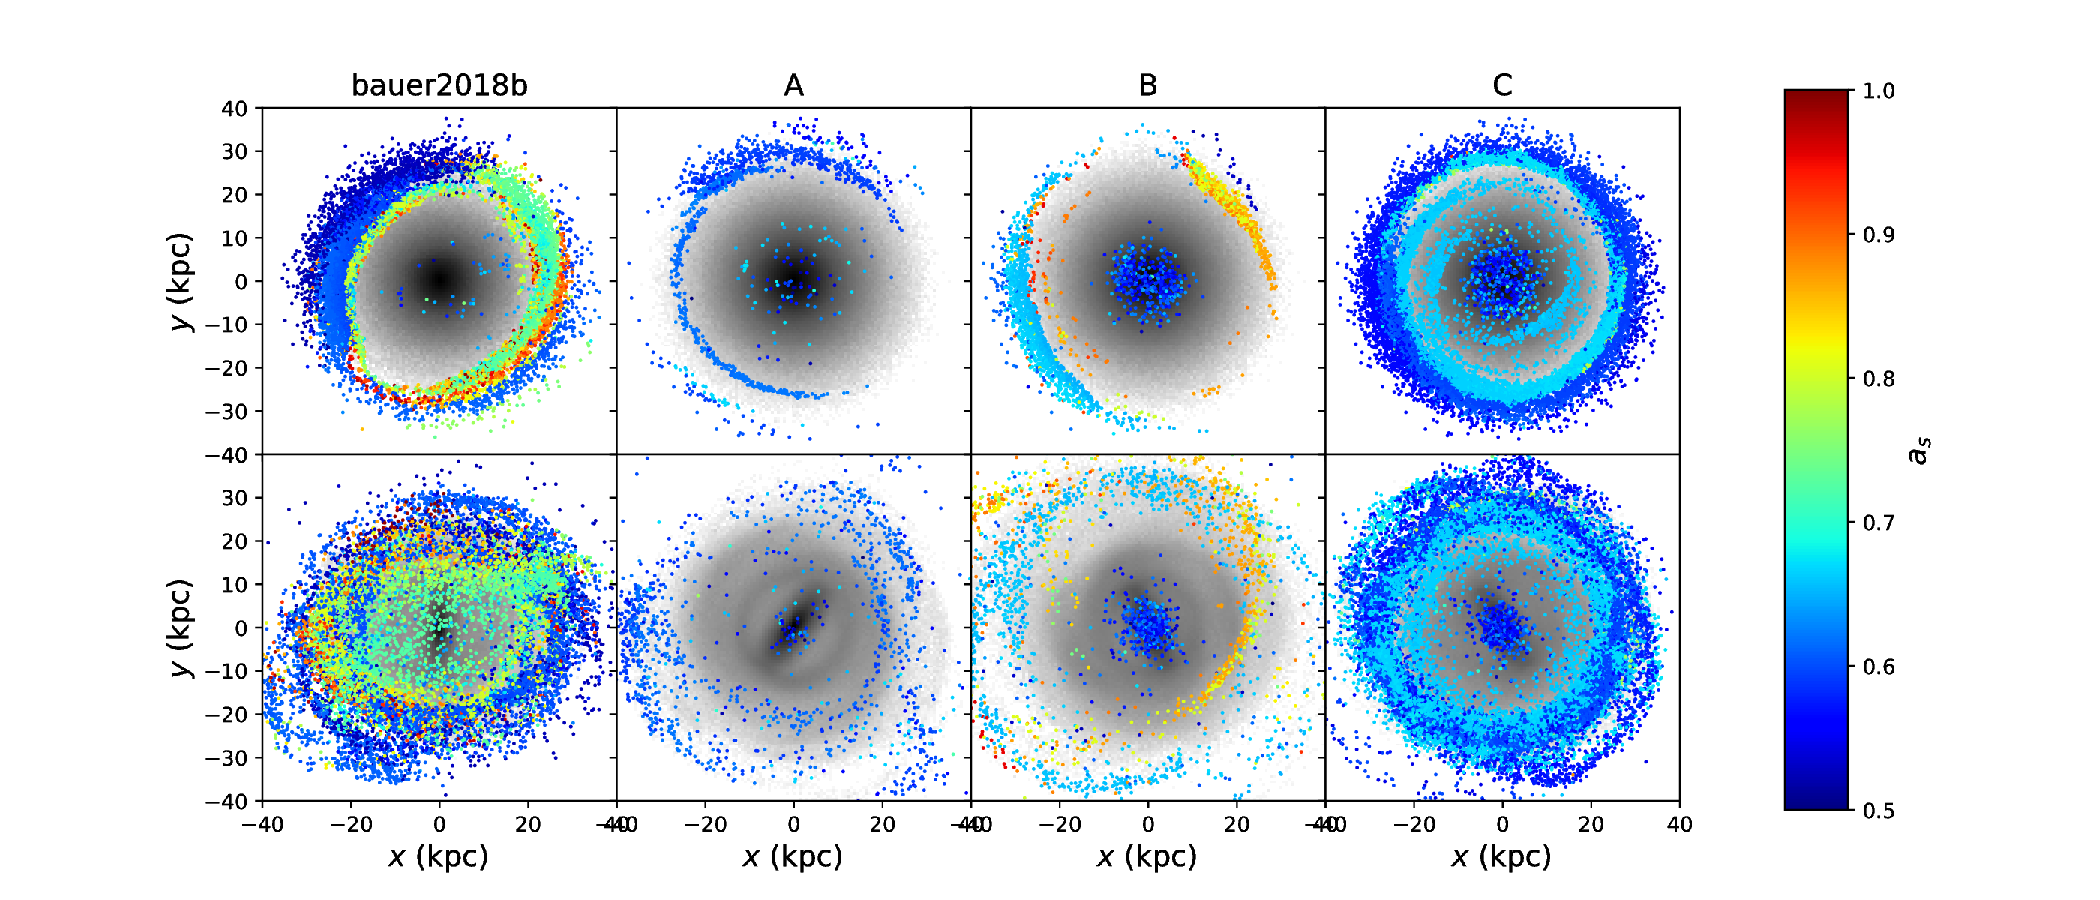
\includegraphics[width=0.9\textwidth]{../figures/kud_early_insert_face_on.pdf}}\\ 
    \subfloat[]{\includegraphics[width=0.9\textwidth]{../figures/kud_early_insert_edge_on.pdf}} 
\caption{KOD stars are shown for the fiducial suite in face-on (a) and
  edge-on (b) projections in the initial disc (upper panel) and final
  snapshot (lower panel). The stars not kicked out of the disc are
  shown as a histogram and the KOD stars are coloured by the time
  satisfying Eq. \ref{eq:kud_def}. Each column is one of the haloes
  considered in this paper.}
	\label{fig:kud_stars_final_ics}
\end{figure*}
We a define a kicked-out star as one where the distance from the
midplane, $|z(t)|$, exceeds some threshold, $\eta z_{\rm rms}$:
\begin{equation}
|z(t)| > \eta\,z_{\rm rms}(t)\label{eq:kud_def}
\end{equation}
where $\eta$ is a dimensionless parameter and $z_{rms}(R,\,t)$ is the
time-dependent thickness of the disc, as estimated in an annulus at
$2.2R_d$. Clearly, the choice of $\eta$ determines the number of stars
identified as being kicked out of the disc. For example,
$\eta=4$ yields 216K KOD stars or $6.2\%$ of the total stellar
content of the disc. Likewise, $\eta=8$ and $\eta=12$ yield 19K KOD
stars ($0.53\%$) and 4,302 KOD stars ($0.069\%$), respectively. These
percentages can be compared with the percentages of stars in an
exponential disc that satisfy our KOD criteria, namely
$1.8\%,\,0.034\%$, and $6\times 10^{-4}\%$, for $\eta=4,\,8,$ and
$12$, respectively. We see that for $\eta=8$ and $\eta=12$, the
number of stars identified as being kicked out exceeds the number
expected in an exponential disc by over an order of magnitude.

\begin{figure}
    \centering
    \includegraphics[width=0.85\textwidth]{../figures/fiducial_halo_268824_xy_s_016.pdf}
	\caption{KOD stars are plotted for C.Early at the labeled
          times. Note the association with spiral arms, suggesting a
          similar mechanism to \citet{laporte_2019_feathers}.}
	\label{fig:xy_tidal_tail_halo_c}
\end{figure}

\begin{figure}
    \centering
  	\subfloat[]{\includegraphics[width=0.85\textwidth]{../figures/fiducial_halo_268824_lb_s_055_overlay.pdf}\label{fig:lb_halo_c_warm_comparison}}\\
  	\subfloat[]{\includegraphics[width=0.85\textwidth]{../figures/fiducial_halo_268818_late_insert_lb_s_095_overlay.pdf} \label{fig:lb_halo_b_late}}
	\caption{Heliocentric views of KOD stars in several different
          distance shells. The top panel depicts this for C.Early at
          $a=0.775$. The bottom panel shows the same for B.Late at
          $a=0.975$.}
\end{figure}

\subsection{KOD Star Dynamics} \label{ssec:kud_dynamics}

We now turn our attention to the dynamics of KOD stars, identified via
Eq. \ref{eq:kud_def} with $\eta=8$ in the final
snapshot. Fig. \ref{fig:kud_stars_final_ics} shows the KOD stars in
our fiducial suite at the final snapshot. In addition, we show the
same stars traced back to their position in the initial snapshot. The
stars are color-coded by the time at which they are kicked out of the
disc.  We immediately see that the KOD structures vary markedly across
our simulations. For example, A.Early shows a relatively small KOD
population.  Moreover, the KOD structure it does have exists at very
low latitudes and was kicked out fairly early in the
simulation. B.Early has a few streams of KOD stars, which were kicked
out of the disc at roughly the time when the disc had its close
encounters with massive subhalos. Indeed, there appear to be two
distinct populations of KOD stars. Finally, bauer2018b.Early and
C.Early show the most significant populations of KOD stars.  These
simulations correspond to the simulations with the most significant
disc-halo misalignment and shortest $T_\tau$. In both cases, we see a
continuous range of times over which stars were kicked out. Moreover,
in C.Early, many of the KOD stars were originally in the inner disc.

The mechanism in C.Early by which stars from the inner disc can be
kicked out is highlighted in Fig. \ref{fig:xy_tidal_tail_halo_c}. Each
new round of KOD stars appears to be associated with a spiral pattern
of small pitch angle. Together with
Fig. \ref{fig:kud_stars_final_ics}, we are left with the picture that
KOD stars generally originate in the outer disc though in some cases,
such as C.Early, strong spiral structure transfers stars outward and
into strong warps. Stars in these warps can then be easily stripped
from the disc. The stripped stars in turn phase mix to form the
high-latitude structures seen in the final snapshot of C.Early.  Stars
associated with the features seen in
Fig. \ref{fig:xy_tidal_tail_halo_c} form filamentary structures with a
characteristic bifurcation, which \citet{laporte_2019_feathers}
referred to as ``feathers".

In Fig. \ref{fig:lb_halo_c_warm_comparison}, we see the KOD stars in
C.Early as they appear from the Solar neighborhood at $a=0.775$. The
stars form the top and bottom feather structure described in
\citet{laporte_2019_feathers}, and are undoubtedly associated with
grand design spiral structure. The similarities suggest that
large-scale tidal fields create observable, stream-like structures at
low-to-mid Galactic latitudes, extending along the length of the sky.
We contrast this with B.Late, where there is a moderate-mass
($10^{10}\,M_\odot$) Sgr interaction. From the perspective of the Sun,
KOD structures present in B.Late and shown in
Fig. \ref{fig:lb_halo_b_late} appear at relatively low latitudes. Thus
a moderate-mass Sgr dSph does not appear to be capable of exciting
high latitude structures on a short timescale.

\section{Discussion} \label{sec:discussion}

\subsection{Disc Flapping}

Perhaps the most novel effect that we have explored is the generation
of flapping modes from differential acceleration of the disc by
distant subhalos and other mass concentrations in a $\Lambda$CDM cosmology.
\citet{sellwood_1996} presented the first in-depth study
of this phenomenon in isolated galaxies. We find that the disc
flapping naturally arises in the cosmological environment and can be
due to one of three mechanisms: two-body interaction of the 
disc and inner halo with a subhalo, buckling of the bar,
and torquing of the disc by its smooth, triaxial halo.

There is reason to think that the first of these mechanisms is is
secondary to the others. \citet{gomez_2017} ran MHD simulations
where they note a lack of U-shaped ($m=0$) warps, which would
presumably be caused by flapping. Conversely, they found that S-shaped
($m=1$) warps were fairly common. In our suite of simulations, B.Late
provides the best example where flapping modes from a distant subhalo can be seen as the
dominant effect; it has no buckling bar and is initialized in a quiet
halo. For both A.Early and C.Early, we would be hard pressed to say
that we see the same kind of behaviour, especially where the disc is
decently resolved.

The bar buckling generation mechanism for flapping modes is
prominently displayed in C.Early. After the bar buckles, we see
axisymmetric fluctuations in the mean height, as well as substantial
flapping in the region of Monoceros. C.Early is clearly an outlier in
this respect, and we suggest that bar buckling in conjunction with
triaxility is a viable mechanism for corrugations in cosmological
simulations. The general effect of bar buckling appears to introduce a
signal in mean height, consistent with the simulation in
\citet{bar_buckling_echo}.

\subsection{Bending waves, KOD stars and feathers}

Consistent with \citet{gomez_2017}, we find that halo misalignment is
not a likely source of bending in the inner disc. Rather, most of the
$m=0$ and $m=1$ waves in the inner disc appear to be associated with
bar buckling. However, the outer disc is most definitely affected by
the smooth halo's tides. We see this in C.Early's $m=1$ profile, which
is much stronger than that in either B.Late or A.Early.

\citet{laporte_2018_b} and \citet{laporte_2019_feathers} found that a
massive Sgr-like dwarf ($M \simeq 8 \times 10^{10} \, \solarm$ and
above) whose orbit passes through the Galactic midplane several times
can produce populations of KOD stars consistent with those observed
in the Milky Way. It is worth noting that their proposed mass is at
the higher end of estimates for the mass of the Sgr dSph
progenitor, and twice the mass of the stellar disc in our simulations. Our B.Late simulation provides an example of an encounter
with a $3 \times 10^{10}$ subhalo that passes through the disc plane
at $a=0.875$ on an orbit that is similar to model L1 in
\citet{laporte_2018_b}. Consistent with their findings, it appears
that even this quite massive perturber cannot excite the requisite
structures. On the other hand, we do find KOD stars in other
simulations within our suite where the main disc-environment effects
come from large-scale tidal fields. Indeed, the simulations in which
KOD stars reach their highest latitudes are the ones with substantial
inner-halo-disc axis misalignment, namely C.Early and
bauer2018b.Early. These are also the simulations with the highest
$m=1$ bending signature in the outer disc.  Thus, kicking stars to
higher latitudes either requires an extremely massive perturber or
substantial misalignment with the host halo.

Our results are consistent with those of \citet{laporte_2019_feathers}
who found that KOD stars remain close to each other in phase space. For
instance, in B.Late stars are kicked out of the disc at two discrete
times from narrow regions of the disc. By the end of the simulation,
these stars are still closely associated with each other.  We can also
infer from our simulations that for some mono-abundant chemical
population at $z=1$, we would expect to see dynamically coherent (as
supported by how stars are clustered by their kick-up time in the
final snapshot) structures with a consistent chemical abundance. This
result is consistent with observations by \citet{bergemann_2018}, who
found narrow abundance spreads for M-giants in A13 and TriAnd. The
clustering of stars by their kickup time is true whether they were
kicked by substructure, as in B.Late, or by the smooth halo, as in
C.Early.

\section{Conclusions}\label{sec:conclusion}
{We have presented a suite of simulations in which stellar discs are
inserted into cosmological haloes. These halos are, in general,
triaxial and clumpy and drive the disc from its initial axisymmetric
and near equilibrium state to one of disequilibrium. The key findings are summarized as:
\begin{itemize}
\item All discs all form bars, even though buckling can regulate their strengths.
\item All discs exhibit some kind of bending and warping.
\item Disc flapping is a major manifestation of disequilibrium in the cosmological environment.
\item Subhaloes with a mass lower than that of the disc are unlikely to generate KOD populations.
\end{itemize}}
{It is not surprising that} the discs in our simulations bend and warp. In
addition, we find large populations of stars kicked out of the disc.
These departures from planarity signal a state of disequilibrium {likely present in the Milky Way}.  We
have identified several mechanisms for generating vertical structure, which
include the well-studied interaction of the disc with a massive
satellite, differential acceleration of the disc due to tidal fields
of the halo or a distant massive satellite, and the buckling bar.
The first two mechanisms can produce large warps (amplitudes of
order 1-3 kpc) in the outer disc along with smaller amplitude 
waves that extend further in. On the other hand, the buckling bar
is efficient at producing bending waves and corrugation patterns 
in the inner disc.

{Absent substantial global tides, the KOD populations we see are not able to reach high latitudes. As such, o}ur findings are consistent with the idea that a subhalo less
massive than the disc is unlikely to be responsible for even low
latitude streams seen in the Milky Way. On the other hand, disc-halo
misalignment can generate these populations quite easily. {Taken in whole, our analysis suggests that studies which focus on only one mechanism of vertical structure generation are unlikely to capture the full picture. We have done out best to disentangle the different mechanism of disequilibrium. Future work will attempt to determine which ones dominate in the Milky Way.}

\section*{Acknowledgements}
{LMW and JSB are supported by a Discovery Grant with the Natural
  Sciences and Engineering Research Council of Canada.}
  
  
\bibliographystyle{apalike}
\bibliography{bibliography_paper_iii.bib} % if your bibtex file is called example.bib


%%%%%%%%%%%%%%%%%%%%%%%%%%%%%%%%%%%%%%%%%%%%%%%%%%




%\chapter{Alloy}\label{ch:Alloy}

\section{The Alloy Language}

    %\gloss{Alloy} is...
    Alloy is...

\paragraph{Quantifiers}

        There are five quantifiers available in Alloy:

        \begin{center}
        \begin{singlespacing}
        \begin{tabular}{|l|l|} \hline
        % after \\: \hline or \cline{col1-col2} \cline{col3-col4} ...
        \multicolumn{1}{|c|}{Quantifier} & \multicolumn{1}{c|}{Meaning} \\ \hline
        \texttt{all x :~e | F} & universal, \texttt{F} is true for every \texttt{x} in \texttt{e} \\
        \texttt{some x :~e | F} & existential, \texttt{F} is true for some \texttt{x} in \texttt{e} \\
        \texttt{no x :~e | F} & \texttt{F} is true for no \texttt{x} in \texttt{e} \\
        \texttt{sole x :~e | F} & \texttt{F} is true for at most one \texttt{x} in \texttt{e} \\
        \texttt{one x :~e | F} & \texttt{F} is true for exactly one \texttt{x} in \texttt{e} \\ \hline
        \end{tabular}
        \end{singlespacing}
        \end{center}


\subsubsection{Signatures and Fields}

        The simple signature \verb|sig A {}| introduces \texttt{A} as a basic type with a set
        of atoms of that type.  \texttt{A} refers to the set of atoms; the type is inferred
        by Alloy and cannot be referenced explicitly.

        \begin{singlespacing}
        \begin{verbatim}
        sig A {}
        sig B {
            f : A
        }        \end{verbatim}
        \end{singlespacing}


\subsection{Example}\label{sec:firstAlloyExample}

    An excerpt from an Alloy
    specification of a singly-linked list is presented in
    Listing~\vref{list:simpleLinkedList}.

    \begin{Listing}
    \begin{singlespacing}
    {\small
    \begin{verbatim}
    sig Node {                    sig List {
        next : option Node            first : Node
    }                             }{
                                      all n : Node | n in first.*next
                                      no n : Node | n in n.^next
                                  }    \end{verbatim}
    }
    \caption{Excerpt of a simple Alloy specification for a singly-linked list}
    \label{list:simpleLinkedList}
    \end{singlespacing}
    \end{Listing}


%\chapter{Embee: User Perspective}\label{ch:Embee1}

    \begin{Listing}[H]
    \filein{Examples/List.als}
    \caption{Alloy specification of a singly-linked list using only binary relations}
    \label{list:SimpleList1}
    \end{Listing}


\subsection{Phase 1: High-Level Static Mapping}\label{sec:phase1}

    ...Phase 1 simply generates the default static
    mapping and presents it to the user, as shown in Figure~\vref{fig:defaultMap}.  We
    have modified the map file as shown in Figure~\vref{fig:fixedMap}.

    \begin{figure}[H]
    \begin{singlespacing}
    \centering
        \subfigure[Default static mapping]{
            \begin{minipage}{2.25in}\footnotesize
                {\texttt{List = List\\
                List\$first =
                List.first\\
                Node = Node\\
                Node\$next = Node.next\\
                }
                }\label{fig:defaultMap}
            \end{minipage}}
        \subfigure[Modified static mapping]{
            \begin{minipage}{2.25in}\footnotesize
                {\texttt{List = SimpleList\\
                List\$first = SimpleList.first\\
                Node = Node\\
                Node\$next = Node.next\\
                }
            }\label{fig:fixedMap}
            \end{minipage}}
    \caption[Excerpt of high-level static mapping file]{Excerpt of high-level static
    mapping file before and after modification}
    \end{singlespacing}
    \end{figure}



    Figure~\vref{fig:tree_beforeAndAfter} shows the tree
    before and after deletion, with correctly implemented code.
    Figure~\vref{fig:tree_commentedOut_mainBody} shows the tree after deletion of the
    root, when the \texttt{root = n2} statement is not executed.

    \begin{figure}[H]
    \centering
    \mbox{
        %\subfigure[Before deletion]{\includegraphics[scale=0.65]{Figures/correct_pre.eps}}\label{fig:tree_correct_pre}
        %\subfigure[After correct deletion]{\includegraphics[scale=0.65]{Figures/correct_post.eps}}\label{fig:tree_correct_mainBody}
        \subfigure[Before deletion]{\includegraphics[scale=0.65]{Figures/correct_pre}}\label{fig:tree_correct_pre}
        \subfigure[After correct deletion]{\includegraphics[scale=0.65]{Figures/correct_post}}\label{fig:tree_correct_mainBody}     
        }
    \caption[Visualization of tree]{Visualization of tree before and after correct deletion of the root node}
    \label{fig:tree_beforeAndAfter}
    \end{figure}

    \begin{singlespacing}
    \begin{figure}[H]
    \centering
    %\includegraphics[scale=0.75]{Figures/commentedOutWithBetterNumber_post.eps}
    \includegraphics[scale=0.75]{Figures/commentedOutWithBetterNumber_post}
    \caption[Visualization of tree after deletion of root (error or omission)]{Visualization of tree
    after deletion of the root node, with an error of omission in the code.
    \texttt{Node\_7} represents the temporary node in the \texttt{swapNodes()} method.}
    \label{fig:tree_commentedOut_mainBody}
    \end{figure}
    \end{singlespacing}

%\chapter{Embee: Implementation and Analysis}\label{ch:Embee2}


    \begin{singlespacing}
    \begin{Listing}[h]
    \fileinsmall{Examples/connectToVM.txt} \caption[Excerpt from
    \texttt{StateDumperThreads.java}]{Excerpt from \texttt{StateDumperThreads.java},
    showing how to connect to a second virtual machine executing the target code.  In
    this example, the target class is referenced by \texttt{javaClassName}.  The JPDA
    classes can be accessed by including the \texttt{tools.jar} archive in the program's
    classpath; this archive is found in the Java installation's \texttt{lib} directory}
    \label{list:connectToVM}
    \end{Listing}
    \end{singlespacing}


    \begin{figure}[h]
    \begin{singlespacing}
    \centering
        \subfigure[Specification of binary \texttt{next} relation]{
            \begin{minipage}{100pt}
                \filein{Examples/smallA.txt}
            \label{fig:smallBinary}
            \end{minipage}}
        \hspace{0.25in}
        \subfigure[Implementation of binary relation in (a)]{
            \begin{minipage}{100pt}
                \filein{Examples/smallB.txt}
            \label{fig:smallBinaryCode}
            \end{minipage}}
        \hspace{0.25in}
        \subfigure[Specification of ternary \texttt{next} relation]{
            \begin{minipage}{100pt}
                \filein{Examples/smallC.txt}
            \label{fig:smallTernary}
            \end{minipage}}
    \caption[Sample specification and implementation]{Sample specification and
    implementation of a binary relation; sample specification of a ternary relation}
    \end{singlespacing}
    \end{figure}

\section{Complexity and Performance}\label{sec:EmbeeComplexity}

\subsection{Definition of Terms}\label{sec:termDefn}

    The following terms...:

    \begin{Ventry}{\boldmath $\operatorname{arity}(r_i)$ \unboldmath}

        \boldmath \item[$scope$] \unboldmath
        The maximum number of objects...

        \boldmath \item[$R$] \unboldmath
        The number of relations...

        \boldmath \item[$r_i$] \unboldmath
        The $i^\text{th}$ relation in the specification, $1 \le i \le R$.

        \boldmath \item[$\operatorname{arity}(r_i)$] \unboldmath
        The arity of relation $r_i$...

        \boldmath \item[$N$] \unboldmath The total number...

        Given the calculated arities of a particular specification's relations, and the scope at
        a specific breakpoint, Equation~\ref{equation:N} can be used to determine $N$.
        \begin{equation}\label{equation:N}
        N = S \times scope + \sum_{i=1}^R scope ^ {arity(r_i)}
        \end{equation}

    \end{Ventry}



    The combined complexity of all four steps is
    \begin{equation*}
        O(N) + O(nN) + O(N^2) + O(F)
    \end{equation*}
    Again, these steps are completed once for every breakpoint in the target program's
    execution; therefore, the overall upper bound becomes
    \begin{equation*}
    \begin{split}
        & b \times O(N) + b \times O(nN) + b \times O(N^2) + b \times  O(F) \\
                   = ~ & O(bN + bnN + bN^2 + bF)
    \end{split}
    \end{equation*}


    The vector [$x_0$  $x_1$] represents the two possible atoms of type
    \texttt{X}.  With our naming scheme, $x_0$ represents \texttt{X\_0} and $x_1$
    represents \texttt{X\_1}.
    The binary relation itself is represented by a two-dimensional bit matrix where a 1 in
    position [$i$,$j$] means that there is a mapping between the $i^{th}$ atom of \texttt{X}
    and the $j^{th}$ atom of \texttt{Y}:

    \begin{gather*}
    \begin{bmatrix}
      r_{00} & r_{01} \\
      r_{10} & r_{11} \\
    \end{bmatrix} \quad
    \begin{bmatrix}
      \texttt{X\_0->Y\_0} & \texttt{X\_0->Y\_1} \\
      \texttt{X\_1->Y\_0} & \texttt{X\_1->Y\_1} \\
    \end{bmatrix}
    \end{gather*}
    \medskip

    Now, consider a fact stating that relation \texttt{r} is total, i.e.,

    \begin{center}
    \texttt{all x :~X | some y :~Y | x.r = y}
    \end{center}

    The CNF formula for our example fact, in scope~2, is
    \begin{equation*}
    \begin{split}
    & \neg(((x_0 \wedge r_{00}) \vee (x_1 \wedge r_{10})) \wedge \neg((x_0 \wedge r_{01})
    \vee (x_1 \wedge r_{11}))) \wedge \\ &\neg(\neg((x_0 \wedge r_{00}) \vee (x_1 \wedge
    r_{10})) \wedge ((x_0 \wedge r_{01}) \vee (x_1 \wedge r_{11})))
    \end{split}
    \end{equation*}
    \medskip

    Table~\vref{fig:fullRunTimesAllPhases} contains...

    \begin{singlespacing}
    \begin{center}
    \begin{threeparttable}
    \caption{Running times for each phase and total running time of Embee}
    \label{fig:fullRunTimesAllPhases}\begin{small}
        % Table generated by Excel2LaTeX from sheet 'Embee'
        \begin{tabular}{|l|c|c|c|c|c|c|c|} \hline

        \multicolumn{3}{|c|}{Test Case} & \multicolumn{ 5}{c|}{Running Time (m:ss)} \\ \hline

        \multicolumn{1}{|c|}{Object} & & Number of & & & \multicolumn{2}{c|}{ Phase 3} &  \\  \cline{6-7}

        \multicolumn{1}{|c|}{Model} & \raisebox{1.5ex}[0pt]{Scope} & Breakpoints &  \raisebox{1.5ex}[0pt]{Phase 1} & \raisebox{1.5ex}[0pt]{Phase 2} &   First 16 &   Last 4 &  \raisebox{1.5ex}[0pt]{Total} \\

        \hline
            List  &  20 &  20           &  0:07 &  0:32 &  0:12 &  06:39 & 07:30 \\
        \hline
            Graph &  20 &  19\tnote{a}  &  0:07 &  1:27 &  0:35 &  44:10 & 46:19 \\
        \hline
            Tree  &  20 &  20 &  0:04   &  1:20 &  0:21 &  06:04 &  07:49 \\
        \hline
        \end{tabular}
    \begin{tablenotes}
    \item[a] Breakpoints occur after the addition of each edge, i.e., the first
    breakpoint does not occur until the second node is added.
    \end{tablenotes}
        \end{small}
    \end{threeparttable}
    \end{center}
    \end{singlespacing}


    ...upper bound on Embee's performance:

    \begin{numcases}{\text{upper bound is}}
        O(bN^2) & if $scope \leq 16$ \notag \\
        O(bF)   & if $scope > 16$ \notag
    \end{numcases}



\chapter{Summary and Conclusions}\label{ch:conclusion}
\newpage


In this chapter, we summarize the  main findings of this thesis and talk about future work.


\section{Disc-Halo Interactions}


\subsection{Summary}

One of the key contributions of this thesis is the understanding of how the dynamic nature of stellar discs affects halo properties, as studied in Chapter~\ref{ch:paper_i}. Some halo properties, such as the distribution of mass in the inner halo, depend a lot on how the disc is modelled. This is very evident in the differences in adiabatic contraction between the rigid and live discs. Specifically, we find the formation of a bar led to a more concentrated halo mass distribution. On the whole, these results suggest that if one is interested in the Core-Cusp problem, this should be studied with fully live models of stellar discs.

The intermediate-to-outer halo is less effected by the dynamics of the inner halo. While some differences between our disc potential models were observed in the halo mass functions, these differences were minor. The details of how satellites are disrupted appear to be at least weakly dependent on how the disc is modelled, and stream studies should consider as realistic of a disc as possible. This last aspect of our work has informed some design decisions by others, namely in the work of \citet{read_2019}. If one is just interested in subhalo population statistics, it is sufficient to model baryons as fixed potentials in a pure dark matter halo.

The global picture painted by our work is that modelling the disc as a rigid body does well in determining how the disc settles (i.e. its angular motion), a result consistent with \citet{DubinskiKuijkenRigidDisks}. It appears that the formation of a bar in the live disc is the most substantial difference between the rigid and live discs' effects on the inner halo, a difference that only becomes significant \textit{after} the the live disc



%Beyond the effect of the disk on the halo, we find that our rigid disk approximation is quite realistic in modelling the angular evolution of the disk. This allows us to set up near-equilibrium cosmological systems without the use of MHD simulations. Since the work in this thesis focuses on the underlying theoretical mechanisms driving the evolution of galaxies in cosmological environments, we only need a good representation of the true systems.

\subsection{Insertion Scheme and Future Work} \label{ssec:conclusions_insertion}

Our algorithm makes optimizations over previous disc insertion schemes. The optimizations we made are by no means exhaustive, and a detailed discussion of potential optimizations is given in Chapter~\ref{ch:implementation}. We focus here on scientific concerns with our algorithm, rather than performance optimizations. 

The scheme as specified has the undesirable property of adding angular momentum and mass to the halo. This happens when the disc grows, and we fail to extract mass and angular momentum from the halo\footnote{Note that dark matter particles dark matter only simulations include the baryon mass of the Universe.}. A potential improvement which extracts mass and angular momentum from the halo particles during the disc growth phase would alleviate these concerns. This may have a sizable impact on our conclusions about the disc's effect on adiabatic contraction, since both the disc and halo are dominant in the inner galaxy.

We might also consider a scheme which initializes the disc with some gas component. \citet{deg_2019} modified \textsc{GalactICS} to allow for the inclusion of gas. This, combined with modifying halo particle masses, should allow us to more accurately compare our results to fully hydrodynamical \textit{ab initio} simulations.

A valid criticism of our disc insertion technique is that all of the stars are initialized simultaneously. This is unrealistic, and allowing stars to gradually form out of the rigid disc potential might show a more complicated dependence on the initial conditions parameter space. In fact, \citet{aumer_2016} grow discs in a similar fashion and find that slowly growing the disc along with gas physics impacts important properties like bar formation. In some cases it may even shut off bar formation, which we believe would substantially impact our conclusions about adiabatic contraction.

Even with the current algorithm, there is more we can do on the study of disc-halo interactions. A possible project would be to study the effect of varying disc properties in the same halo. We might also consider adding a spheroidal bulge component to see how high baryonic mass concentrations change our results. We might also look for more detailed evidence of the halo's response to the disc in our existing simulations in the form of wakes. This kind of response was explored in one of our toy models in Chapter~\ref{ch:paper_iii}, and it seems natural to extend this analysis to our cosmological simulations.


\section{Bar Formation}
\subsection{Summary}

We discuss our contributions to understanding how bars form in stellar discs in Chapter~\ref{ch:paper_ii}. The paper unifies previous work on disc insertion schemes by viewing them through a lens of a common parameter space. Through placing our models and the models of \citet{YurinSpringelStellarDisks} in this space, we are able to contextualize the very large bars formed in their study. In particular, we show that a commonly discounted variable, the disc thickness, is a primary driver of bar strength in a cosmological setting. We show that, in general, the length of a bar at present day for cosmological stellar discs is largely a function of the initial disc thickness. This effect is not numerical, as we show through our application of the \textsc{AGAMA} code \citep{vasiliev_2018}. 

The importance of being cautious about the choice of gravitational softening length is also illustrated. Since disc thickness appears to play a major role in bar formation in $\Lambda$CDM, we must be careful that we are resolving our discs' vertical structure.


On the whole, we show that it is difficult to suppress the formation of bars in a cosmological setting. While the bar more closely resemble the Milky Way's when we start with a thinner disc, we find strong bars form nonetheless. As such, there is still a discrepancy in accounting for the observed bar fraction without invoking classical bulges or non-collisionless phenomena. Our work has proved useful in illustrating this, and we are credited for furthering discussion of this issue in \citet{sellwood_2019}.


We manage to bolster this result in Chapter~\ref{ch:paper_iii}, where we ran twelve simulations in four halos. Although all of the halos had the same total mass as the Milky Way, they varied widely in terms of their other properties. Despite the differences in the halos, the bars formed by embedded discs were quite similar. Additionally, there is a nontrivial dependence on Toomre $Q$ in terms of when the bar buckles, but the final bar strength depends very weakly on this parameter, contrary to \citet{YurinSpringelStellarDisks}. Rather, the trend \citet{YurinSpringelStellarDisks} sees in $Q$ is likely due to the presence of their bulge simulations, which would increase $Q$ as well as provide a stabilizing central mass.


\subsection{Further Exploration}


In Chapter~\ref{ch:paper_iii}, bar formation is not the focus of the study. Now that we have a sample of bars forming in different cosmological environments, we can position the discs in the parameter space described in Chapter~\ref{ch:paper_ii}. A proper synthesis with previous literature on this topic should be performed.

An interesting feature of our simulations is the existence of ``banana bars" in some of the simulations. Understanding why we get banana bars in some simulations versus a more traditional X-shaped pattern might provide an observational constraint for the Milky Way. This topic should be explored in more detail.

It would also be interesting to see how implementing a hydrodynamical, growing disc described in \S\ref{ssec:conclusions_insertion} would change our results. An interesting conclusion from \citet{aumer_2016} was that bar formation could be suppressed by GMCs. It is worth noting that these simulations also included a compact bulge, and the result might be different for a pure disc-halo system in a fully cosmological environment. The author's view is that moving in this direction is the next logical step for disc-insertion schemes. 



\section{Vertical Structure}
\subsection{Summary}

The main focus of Chapter~\ref{ch:paper_iii} is how discs form vertical structure in $\Lambda$CDM environments. We showed that there are a wide variety of Milky Way-mass halos that form vertical structure consistent with structure observed in the solar neighborhood. In particular, we showed that this structure can be formed without a massive satellite encounter in a cosmological setting. This position is bolstered by the fact that we see Monoceros-like structure in all twelve of our simulations.

We also find that consistent perpendicular torques on the disc are required to explain features in the outer disc. It is unlikely that substructures far below the $10^{11}$ solar mass regime are responsible for stars stripped to higher latitudes. Global tides from disc-halo axis misalignment seem to be the most effective way to create these populations of stars. We therefore suggest that streams originating from the outer disc may primarily depend on the Milky Way's interaction with the LMC. A massive merger like the one with the LMC can cause consistent perpendicular torques its own tides or by disturbing the existing smooth Milky Way halo mass. 

\subsection{More Accurate Milky Way Comparisons}

A key flaw in this work is that we had no LMC analogues. An interesting experiment would be to compare the vertical structure caused by a future LMC merger and the vertical structure generated when a disc is misaligned in a triaxial halo. On the whole, future work should proceed in the same way as the work in Chapter~\ref{ch:paper_ii}. We should seek to relate the halo environments to a common parameter space.

We also might want to compare our simulations in the solar neighborhood to Gaia data through simulation-generated mock catalogues. Although not presented in this thesis, we have developed a code which allows us to generate initial conditions that are selectively upsampled in a specified annulus. In isolated galaxy simulations, the upsampled annulus remains mostly uncontaminated at late times. By resampling the solar neighborhood, and by using simulation-generated mock catalogues, we can compare our simulations more directly with observations.

\section{Closing Remarks}

%This thesis considered a very specific approach to understanding a very specific concept: the collisionless evolution of systems with stellar disks and dark matter halos. It is tremendously humbling to note that we never even considered gas dynamics, a cosmology other than $\Lambda$CDM, or even systems with a strong, pre-existing bulge. In the end, we were able to make some elucidating comments on the nature of stellar dynamics in $\Lambda$CDM cosmology, but no more. 

This work presents an improved disc insertion scheme with applications to Galactic astronomy. We have successfully shown that we can set up and understand discs inserted into cosmological halos. Future work is suggested, and we have no shortage of potential projects to improve our scheme. The long-term goal of this work is to bridge the gap with \textit{ab initio} simulations, and we have presented a clear roadmap for doing so.

As simulation resolutions and computing power improve, we may be forced to revisit the fundamentals at the beginning of Chapter~\ref{ch:background}. Simulation codes may need to be redesigned to accommodate ever-increasing needs to relate them to observations. Our hope is that disc insertion schemes will be at the heart of these discussions as a valuable tool in understanding observational data.

Our work represents a tangible leap forward, however small, in the field of Galactic dynamics.  We hope that our work continues to inspire new developments, new comparisons, and more questions. In particular, we hope to see our work mature, and possibly tell us about the nature of the dark Universe in which we live. This is an incredibly exciting time for the field, one where we are proud to have played a small role.



\bibliographystyle{apalike}
\bibliography{bibliography_conclusions.bib}
%*************************************************************************************************************
% BIBLIOGRAPHY
%*************************************************************************************************************
% This GATHER command is useful for when you want to use WinEdt's Gather functionality, i.e., type
% \cite{} and a popup box appears with all of your citations to choose from.  Leave the % on the next line.
%GATHER{thesis.bib}

% Put in \nocite{*} so all entries in the bibliography are included
%\nocite{*}

%\bibliographystyle{apalike}
%\bibliography{../bibliography.bib}
\appendix

\definecolor{codegreen}{rgb}{0,0.6,0}
\definecolor{codegray}{rgb}{0.5,0.5,0.5}
\definecolor{codepurple}{rgb}{0.58,0,0.82}
\definecolor{backcolour}{rgb}{0.95,0.95,0.92}


\chapter{Referenced Code: kicks.c} \label{ch:kicks.c}
\lstinputlisting[language=C,basicstyle=\footnotesize,
    commentstyle=\color{codegreen},
    keywordstyle=\color{magenta},
    numberstyle=\tiny\color{codegray},
    stringstyle=\color{codepurple},]{kicks.c}]

\chapter{Referenced Code: predict.c} \label{ch:predict.c}
\lstinputlisting[language=C,basicstyle=\footnotesize,
    commentstyle=\color{codegreen},
    keywordstyle=\color{magenta},
    numberstyle=\tiny\color{codegray},
    stringstyle=\color{codepurple}]{predict.c}]


\chapter{Referenced Code: extract\_halo\_ascii.py} \label{ch:extract_halo_ascii.py}
\lstinputlisting[language=Python,basicstyle=\footnotesize,
    commentstyle=\color{codegreen},
    keywordstyle=\color{magenta},
    numberstyle=\tiny\color{codegray},
    stringstyle=\color{codepurple},]{extract_halo_ascii.py}]
    
    
\chapter{Referenced Code: merge\_ics.cpp} \label{ch:merge_ics.cpp}
\lstinputlisting[language=C++,basicstyle=\footnotesize,
    commentstyle=\color{codegreen},
    keywordstyle=\color{magenta},
    numberstyle=\tiny\color{codegray},
    stringstyle=\color{codepurple},]{merge_ics.cpp}]
    
\chapter{Referenced Code: timestep.c} \label{ch:timestep.c}
\lstinputlisting[language=C,basicstyle=\footnotesize,
    commentstyle=\color{codegreen},
    keywordstyle=\color{magenta},
    numberstyle=\tiny\color{codegray},
    stringstyle=\color{codepurple},]{timestep.c}]

%*************************************************************************************************************
% APPENDICES
%*************************************************************************************************************
\updatechaptername
%\appendixpage
\appendix

%\chapter{Alloy Analyzer}\label{App:AnalyzerCode}

\section{Documentation}

\paragraph*{\large Package: \texttt{alloy.api}}

    %%%%%%%%%%%%%%%%%%%%%%%%%%%%%%%%%%%%%%%%%%%%%%%%%%%%%%%%%%%%
    % AlloyRunner
    %%%%%%%%%%%%%%%%%%%%%%%%%%%%%%%%%%%%%%%%%%%%%%%%%%%%%%%%%%%%
    \begin{singlespacing}
    \begin{center}
    \begin{tabularx}{\linewidth}{|l|X|} \hline
    \multicolumn{2}{|p{420pt}|}{\texttt{\large AlloyRunner}} \\ \hline \hline

    \multicolumn{2}{|p{420pt}|}{\small This class provides...} \\
    \multicolumn{2}{|p{420pt}|}{} \\
    \multicolumn{2}{|p{420pt}|}{\small To do an analysis...}\\ \hline \hline

    {\small \texttt{analyzeCommand}} & {\small Run the actual...} \\ \hline

    {\small \texttt{prepareSpec}} & {\small Parse...} \\ \hline

    {\small \texttt{translateCommand}} & {\small Translate...} \\
    \hline

    \end{tabularx}
    \end{center}
    \end{singlespacing}

%\chapter{Additional Analysis}\label{App:Analysis}

\section{Calculation of Arity}\label{AppSec:arity}


    Examples of arity calculations are shown in Table~\vref{table:arity}.  These calculations
    can be performed using either the equations listed in
    Figure~\vref{fig:arityEquations}...

   \begin{singlespacing}
    \begin{figure}[ht]
    \begin{boxedminipage}[h]{433pt}
        \begin{minipage}{400pt}

        Given:
            \begin{center}
            \begin{minipage}{350pt}
            $v$ is a variable of type \texttt{<var>}, i.e., an \texttt{id} (identifier)\\
            $m$ is a multiplicity expression of type \texttt{<multexpr> }\\
            $r$ is a relation of type \texttt{<relation>}, i.e., $r = v : m$ \\
            $e_1$, $e_2$, ... are expressions of type \texttt{<expr> }in $m$\\
            $x$ is an optional set multiplicity modifier of type \texttt{<setmult>}\\
            $y$, $z$ are optional relation multiplicity modifiers of type \texttt{<mult>}
            \end{minipage}
            \end{center}
        The arity equations are:
        \end{minipage}
        \begin{equation}
        \operatorname{arity}(r) = 1 + \operatorname{arity}(m) \text{,~~where $r$ is of the form $v : m$}
        \label{equation:arity1}
        \end{equation}
        \begin{subequations}
        \begin{numcases}{arity(m)=}
            1 & if $m$ is of the form $x~v$ \label{equation:arity2a} \\
            arity(e_1) + arity(e_2) & if $m$ is of the form $e_1 ~y$ \texttt{->} $z~ e_2$ \label{equation:arity2b}
        \end{numcases}
        \end{subequations}
        \begin{subequations}
        \begin{numcases}{arity(e)=}
            1 & if $e$ is of the form \texttt{id} \label{equation:arity3a} \\
            arity(e_1) & if $e$ is of the form $(e_1)$ \label{equation:arity3b} \\
            arity(e_1) + arity(e_2) & if $e$ is of the form $e_1$ \texttt{->} $e_2$ \label{equation:arity3c}
        \end{numcases}
        \end{subequations}
        \label{equation:arityEquations}
    \end{boxedminipage}
    \caption{Equations to compute arity of relations} \label{fig:arityEquations}
    \end{figure}
    \end{singlespacing}

        \begin{singlespacing}
        \begin{table}[H]
        \begin{center}
        \caption{Example arity calculations}\label{table:arity}
        \bigskip
        \begin{tabular}{|l|c|c|}\hline
        \multicolumn{1}{|c|}{relation $r_i$} & \multicolumn{1}{c|}{$arity(r_i)$} & \multicolumn{1}{c|}{arity equations used} \\ \hline
        \verb|f : A |                    & 2 & \eqref{equation:arity1}, \eqref{equation:arity2a} \\ \hline
        \verb|f : option A|              & 2 & \eqref{equation:arity1}, \eqref{equation:arity2a} \\ \hline
        \verb|f : A -> A|                & 3 & \eqref{equation:arity1}, \eqref{equation:arity2b}, \eqref{equation:arity3a} \\ \hline
        \verb|f : A -> ? B|              & 3 & \eqref{equation:arity1}, \eqref{equation:arity2b}, \eqref{equation:arity3a} \\ \hline
        \verb|f : A -> B -> C|           & 4 & \eqref{equation:arity1}, \eqref{equation:arity2b}, \eqref{equation:arity3c}, \eqref{equation:arity3a} \\ \hline
        \verb|f : A -> B ? -> ! C|       & 4 & \eqref{equation:arity1}, \eqref{equation:arity2b}, \eqref{equation:arity3a}, \eqref{equation:arity3c} \\ \hline
        \verb|f : A -> B -> C -> D|      & 5 & \eqref{equation:arity1}, \eqref{equation:arity2b}, \eqref{equation:arity3c}, \eqref{equation:arity3a} \\ \hline
        \end{tabular}
        \end{center}
        \end{table}
        \end{singlespacing}

\section{Comparison of $N$}\label{AppSec:CompareN}



\subsection{Reasoning about $N$ in terms of $n$}\label{AppSec:Nandn}

    It is possible to determine an upper bound on the size of $N$, relative to the size
    of $n$.  To do this, we re-examine Equation~\ref{equation:N}.

    From Equation~\ref{equation:N}, we have:
    \begin{equation*}
        N = S \times scope + \sum_{i=1}^R scope ^ {arity(r_i)}
    \end{equation*}

    In the worst-case, the scope is equal to the total number of objects that exist at a
    particular breakpoint, i.e., $scope = n$.
    \begin{equation*}
        N = S n + \sum_{i=1}^R n ^ {arity(r_i)}
    \end{equation*}

    We can expand the summation to
    \begin{equation*}
        N = S n + n^{arity(r_1)} + n^{arity(r_2)} + ... + n^{arity(r_R)}
    \end{equation*}

    Because...
    \begin{equation*}
        O(N) = O(S n) + O(n^{arity(r_1)}) + O(n^{arity(r_2)}) + ... +
        O(n^{arity(r_R)})
    \end{equation*}

    We assume that all $R$ relations in the specification have the same arity, and that this
    arity is represented by a value $x \geq 2$.  Therefore...
    \begin{align}
        O(N) & = O(S n) + R \times O(n^x) \notag \\
             & = O(S n) + O(R n^x)
        \label{equation:NwithSR}
    \end{align}

    Equation~\ref{equation:NwithSR} demonstrates...

    Because both $S$ and $R$ are finite numbers, it is possible to further reduce
    Equation~\ref{equation:NwithSR} to
    \begin{align}
        O(N) & = O(n) + O(n^x) \notag \\
             & = O(n^x)
        \label{equation:NwithoutSR}
    \end{align}

    Therefore...





\clearpage
\section{Estimation of $F$}\label{AppSec:F}

    For example, Table~\vref{table:numOperators} contains the values of $F$...

    \begin{singlespacing}
    \begin{table}[H]
    \caption[Estimate of Boolean formula size]{Estimate of Boolean formula size,
    determined by number of Boolean operators (``and", ``or", ``not")}
    \label{table:numOperators}
        \begin{center}

        \bigskip

        % Table generated by Excel2LaTeX from sheet 'formula (extract)'
        \begin{tabular}{|c|r|r|r|r|}
        \hline
            \multicolumn{ 5}{|c|}{\textbf{Example 1 - List}} \\
        \hline
            $scope$ & \multicolumn{1}{c|}{$N$} & \multicolumn{1}{c|}{0 Facts} & \multicolumn{1}{c|}{1 Fact} & \multicolumn{1}{c|}{2 Facts} \\
        \hline
                1 &  4 &    23  &     34  &     43  \\
                2 & 12 &   197  &    657  &    729  \\
                3 & 24 &   671  & 13,799  & 15,200  \\
                4 & 40 & 1,731  & 91,435  & 96,771  \\
        \hline
        \end{tabular}

        \bigskip

        % Table generated by Excel2LaTeX from sheet 'formula (extract)'
        \begin{tabular}{|c|r|r|r|r|r|}
        \hline
            \multicolumn{ 6}{|c|}{\textbf{Example 2 - Graph}} \\
        \hline
            $scope$ & \multicolumn{1}{c|}{$N$} & \multicolumn{1}{c|}{Facts} & \multicolumn{1}{c|}{1 Fact} & \multicolumn{1}{c|}{2 Facts} & \multicolumn{1}{c|}{3 Facts} \\
        \hline
                1 & ---&   ---  &     ---  &       ---  &       ---  \\
                2 & 16 &   185  &   1,005  &     1,783  &     2,181  \\
                3 & 42 &   674  &  66,722  &   118,250  &   142,328  \\
                4 & 88 & 1,787  & 635,811  & 1,153,063  & 1,319,611  \\
        \hline
        \end{tabular}

        \bigskip

        % Table generated by Excel2LaTeX from sheet 'formula (extract)'
        \begin{tabular}{|c|r|r|r|r|r|r|}
        \hline
            \multicolumn{ 7}{|c|}{\textbf{Example 3 - Tree}} \\
        \hline
            $scope$ & \multicolumn{1}{c|}{$N$} & \multicolumn{1}{c|}{0 Facts} & \multicolumn{1}{c|}{1 Fact} & \multicolumn{1}{c|}{2 Facts} & \multicolumn{1}{c|}{3 Facts} & \multicolumn{1}{c|}{4 Facts} \\
        \hline
                1 &  7 &    39  &      78  &      93  &     103  &     104  \\
                2 & 22 &   367  &   1,601  &   2,487  &   2,629  &   2,715  \\
                3 & 45 & 1,283  &  38,528  &  73,472  &  76,196  &  76,568  \\
                4 & 76 & 3,359  & 234,595  & 456,459  & 466,979  & 468,087  \\
        \hline
        \end{tabular}
        \end{center}
    \end{table}
    \end{singlespacing}


\clearpage
\subsection{Test Series}

    Table~\vref{table:tests} summarizes...

    \begin{singlespacing}
    \begin{table}[H]
    \begin{center}
    \caption{Test series for evaluating the running time of conformance checking}
    \begin{tabular}{|c|c|c|c|c|c|c|c|c|} \hline
      % after \\: \hline or \cline{col1-col2} \cline{col3-col4} ...
      Series &  &  &  &  & Number &  &  & Number \\
      Name &
      \raisebox{1.5ex}[0cm][0cm]{Example} &
      \raisebox{1.5ex}[0cm][0cm]{$S$} &
      \raisebox{1.5ex}[0cm][0cm]{$R$} &
      \raisebox{1.5ex}[0cm][0cm]{$\operatorname{arity}(r_i)$} &
      of Facts &
      \raisebox{1.5ex}[0cm][0cm]{$scope=n$} &
      \raisebox{1.5ex}[0cm][0cm]{$N$} &
      of Tests \\ \hline

      E1F0 & 1            & 2 & 2 & 2, 2        & 0 & 1,2,...,40 & 4 - 3,280   & 40 \\ \cline{1-1} \cline{6-9}
      E1F1 & \emph{List}  &   &   &             & 1 & 1,2,...,32 & 4 - 1,984   & 32 \\ \cline{1-1} \cline{6-9}
      E1F2 &              &   &   &             & 2 & 1,2,...,31 & 4 - 1,984   & 31 \\ \hline
      E2F0 & 2            & 2 & 2 & 2, 3        & 0 & 2,3,...,40 & 16 - 65,680 & 39 \\ \cline{1-1} \cline{6-9}
      E2F1 & \emph{Graph} &   &   &             & 1 & 2,3,...,40 & 16 - 33,856 & 39 \\ \cline{1-1}\cline{6-9}
      E2F2 &              &   &   &             & 2 & 2,3,...,34 & 16 - 33,856 & 33 \\ \cline{1-1}\cline{6-9}
      E2F3 &              &   &   &             & 3 & 2,3,...,24 & 16 - 14,448 & 23 \\ \hline
      E3F0 & 2            & 3 & 4 & 2, 2, 2, 2  & 0 & 1,2,...,40 & 7 - 6,520   & 40 \\ \cline{1-1} \cline{6-9}
      E3F1 & \emph{Tree}  &   &   &             & 1 & 1,2,...,40 & 7 - 6,520   & 40 \\ \cline{1-1}\cline{6-9}
      E3F2 &              &   &   &             & 2 & 1,2,...,32 & 7 - 4,192   & 32 \\ \cline{1-1}\cline{6-9}
      E3F3 &              &   &   &             & 3 & 1,2,...,32 & 7 - 4,192   & 32 \\ \cline{1-1}\cline{6-9}
      E3F4 &              &   &   &             & 4 & 1,2,...,32 & 7 - 4,192   & 32 \\ \hline
      \multicolumn{8}{|r|}{Total Number of Tests (Conformance Checks)} & 412 \\ \hline
    \end{tabular}
    \label{table:tests}
    \end{center}
    \end{table}
    \end{singlespacing}

%\addappheadtotoc

%*************************************************************************************************************
% GLOSSARY
% Using a glossary is more than beginners need to know; leaving the packages, etc. here for now.
%*************************************************************************************************************
%\usepackage[nonumberlist]{glossaries}
%\usepackage[refpages]{gloss}  % for my glossary
                              % refpages shows the first page where the term occurs
%-------------------------------------------------------------------------------------------------------------
% Tell Latex to make a glossary
%*************************************************************************************************************
%\makeglossaries  % tell latex to make the glossary
%\glossarystyle{list}

%*************************************************************************************************************
% INDEX
%*************************************************************************************************************
% Here's where the index would be printed, if you created one.  Remove the % on the next line.
%\printindex


%*************************************************************************************************************
\end{document}
